\documentclass[a4paper, 9pt]{scrartcl}\usepackage[]{graphicx}\usepackage[]{xcolor}
% maxwidth is the original width if it is less than linewidth
% otherwise use linewidth (to make sure the graphics do not exceed the margin)
\makeatletter
\def\maxwidth{ %
  \ifdim\Gin@nat@width>\linewidth
    \linewidth
  \else
    \Gin@nat@width
  \fi
}
\makeatother

\definecolor{fgcolor}{rgb}{0.345, 0.345, 0.345}
\newcommand{\hlnum}[1]{\textcolor[rgb]{0.686,0.059,0.569}{#1}}%
\newcommand{\hlstr}[1]{\textcolor[rgb]{0.192,0.494,0.8}{#1}}%
\newcommand{\hlcom}[1]{\textcolor[rgb]{0.678,0.584,0.686}{\textit{#1}}}%
\newcommand{\hlopt}[1]{\textcolor[rgb]{0,0,0}{#1}}%
\newcommand{\hlstd}[1]{\textcolor[rgb]{0.345,0.345,0.345}{#1}}%
\newcommand{\hlkwa}[1]{\textcolor[rgb]{0.161,0.373,0.58}{\textbf{#1}}}%
\newcommand{\hlkwb}[1]{\textcolor[rgb]{0.69,0.353,0.396}{#1}}%
\newcommand{\hlkwc}[1]{\textcolor[rgb]{0.333,0.667,0.333}{#1}}%
\newcommand{\hlkwd}[1]{\textcolor[rgb]{0.737,0.353,0.396}{\textbf{#1}}}%
\let\hlipl\hlkwb

\usepackage{framed}
\makeatletter
\newenvironment{kframe}{%
 \def\at@end@of@kframe{}%
 \ifinner\ifhmode%
  \def\at@end@of@kframe{\end{minipage}}%
  \begin{minipage}{\columnwidth}%
 \fi\fi%
 \def\FrameCommand##1{\hskip\@totalleftmargin \hskip-\fboxsep
 \colorbox{shadecolor}{##1}\hskip-\fboxsep
     % There is no \\@totalrightmargin, so:
     \hskip-\linewidth \hskip-\@totalleftmargin \hskip\columnwidth}%
 \MakeFramed {\advance\hsize-\width
   \@totalleftmargin\z@ \linewidth\hsize
   \@setminipage}}%
 {\par\unskip\endMakeFramed%
 \at@end@of@kframe}
\makeatother

\definecolor{shadecolor}{rgb}{.97, .97, .97}
\definecolor{messagecolor}{rgb}{0, 0, 0}
\definecolor{warningcolor}{rgb}{1, 0, 1}
\definecolor{errorcolor}{rgb}{1, 0, 0}
\newenvironment{knitrout}{}{} % an empty environment to be redefined in TeX

\usepackage{alltt}
\usepackage[ngerman]{babel}

% -----------------------------------------------------------------------


% -----------------------------------------------------------------------
%% ------------------------------------------------------------
%% by J.Kruppa on Friday, February 11, 2022 (11:31)
%% \def\mainDir{\Sexpr{exam_path}}
\def\source{/Users/jokruppa/source/tex}
\usepackage[margin=2cm, includefoot]{geometry}
\setlength{\parindent}{0cm}
\usepackage{booktabs}
\usepackage{amsmath}
\usepackage{scalerel,amssymb}
\usepackage{setspace}
\def\csquare{{\Large $\boxtimes$}}
\def\msquare{{\Large $\square$}}
\usepackage[normalem]{ulem}
\usepackage{array}
\usepackage{xcolor}
\usepackage{float}
\usepackage{currfile}
\usepackage{tikz}
\usepackage[nomessages]{fp}

%% beamer defs
\def\lecture{Klausurfragen der Bio Data Science}

%% exam defs
\def\examtitle{\lecture}
\def\exammodule{
\vspace{-1.75cm}  
\begin{graybox}{}
\vspace{2Ex}
\textbf{\large Name:} \rule[0ex]{16.75em}{.4pt}
\hfill \textnormal{\textit{Nicht bestanden:}} \msquare \\[2.5Ex]
\textbf{\large Vorname:} \rule[0ex]{15em}{.4pt} \\[2.5Ex]
\textbf{\large Matrikelnummer:} \rule[0ex]{10.8em}{.4pt}
\hfill Endnote: \rule[0ex]{7em}{.4pt} 
\end{graybox}
\vspace{3Ex}
\phantom{text}
}
\def\examsemester{Sommersemester \& Wintersemester}
\def\examdate{\today}
%% ------------------------------------------------------------
\definecolor{darkblue}{rgb}{0,0,.5}
\definecolor{darkpurple}{rgb}{0.4117, 0.2, 0.4117}
\definecolor{uni}{rgb}{0,0.3137,0.6078}
\definecolor{gray}{gray}{0.7}

\usepackage{tcolorbox}
\definecolor{logo1}{RGB}{0, 158, 227}
\definecolor{gray5}{RGB}{247, 247, 247}
\definecolor{gray2}{RGB}{102, 102, 102}

\newtcolorbox{graybox}[1]{
  colback=gray5,%%red!5!white,
  colframe=gray2,%%red!75!black,
  fonttitle=\bfseries\Large,
  %%valign=center,
  fontupper=\large,
  before skip=10pt plus 2pt,
  after skip=20pt plus 4pt,
  title=#1}

\newtcolorbox{takehomebox}[1]{
  colback=gray5,%%red!5!white,
  colframe=logo1,%%red!75!black,
  fonttitle=\bfseries\Large,
  %%valign=center,
  fontupper=\large,
  before skip=10pt plus 2pt,
  after skip=10pt plus 2pt,
  title=#1}

\def\Rlogo{
\includegraphics[width = 0.5cm]{\string~/Documents/GitHub/exam/img/Rlogo}\;}

\usepackage[scaled=.90]{helvet} 
\usepackage{fancyhdr}
\usepackage{lastpage}
\usepackage{hyperref}
\hypersetup{
    colorlinks=true,       % false: boxed links; true: colored links
    linkcolor=black,          % color of internal links 
    urlcolor=magenta           % color of external links
}
\renewcommand{\familydefault}{\sfdefault}

\title{
\large \exammodule \\[5Ex]
\Huge \examtitle \\[2Ex] 
\Large Hochschule Osnabr{\"u}ck
}
\author{Pr{\"u}fer: Prof. Dr. Jochen Kruppa \\
Fakult{\"a}t f{\"u}r Agrarwissenschaften und Landschaftsarchitektur \\ 
j.kruppa@hs-osnabrueck.de}
\date{Version vom \examdate}

%% ------------------------------------------------------------
%% by J.Kruppa on Tuesday, September 23, 2014 (12:50)
%% Header
\renewcommand{\headrulewidth}{0pt}
\renewcommand{\footrulewidth}{0pt}
\pagestyle{fancy}

\fancyhf{}
\fancyhead[L]{}
\fancyhead[R]{}
\fancyfoot[R]{\thepage}
\fancyfoot[L]{\footnotesize \examtitle}

\fancypagestyle{empty}{
 \fancyhf{}
 \fancyhead[L]{}
 \fancyhead[R]{}
 \fancyfoot[R]{\thepage}
 \fancyfoot[L]{\footnotesize \examtitle}
}

\usepackage{arevtext,arevmath}

\newcommand\Tstrut{\rule{0pt}{2.6ex}}         % = `top' strut
\newcommand\Bstrut{\rule[-0.9ex]{0pt}{0pt}}   % = `bottom' strut
\def\strut{\Tstrut\Bstrut}

% -----------------------------------------------------------------------
\IfFileExists{upquote.sty}{\usepackage{upquote}}{}
\begin{document}
\date{
\vspace{1.5Ex}
\textbf{\Large\textcolor{red}{>>\underline{\underline{\examsemester}}<<}}
\vfill
\begin{center}

\includegraphics[width = 1.9cm]{avatare/Alex}\hspace{-8mm}

\includegraphics[width = 1.9cm]{avatare/Jessica}\hspace{-8mm}

\includegraphics[width = 1.9cm]{avatare/Jonas}\hspace{-8mm}

\includegraphics[width = 1.9cm]{avatare/Mark}\hspace{-8mm}

\includegraphics[width = 1.9cm]{avatare/Nilufar}\hspace{-8mm}

\includegraphics[width = 1.9cm]{avatare/Paula}\hspace{-8mm}

\includegraphics[width = 1.9cm]{avatare/Steffen}\hspace{-8mm}

\includegraphics[width = 1.9cm]{avatare/Tina}\hspace{-8mm}

\includegraphics[width = 1.9cm]{avatare/Yuki}\\
\small
\vspace{1.5Ex}
\textit{"`The test of a student is not how much she or he knows,\\ but how much the student wants to know."'\\ --- Alice W. Rollins}
\end{center}}
% -----------------------------------------------------------------------
\maketitle
\fancypagestyle{empty}{
  \fancyfoot[L]{\tiny $\square\!\square\!\square\!\blacksquare\!\square\!\square\!\blacksquare\!\blacksquare\!\square\!\square\!\blacksquare\!\square\!\blacksquare\!\square\!\square\!\blacksquare\!\square\!\square\!\square\!\square$}
}
\thispagestyle{empty}
\clearpage
% -----------------------------------------------------------------------
\begin{minipage}[c]{0.125\textwidth}

\includegraphics[width = 1.9cm]{avatare/Alex}
\end{minipage}
\begin{minipage}[c]{0.875\textwidth}
\textit{Alex studiert im 3. Semester und wiederholt das Modul, da er im ersten Jahr andere Prioritäten für sich gesetzt hat. Das musste sein, da er sich ziemlich im Abitur verausgabt hat. Darüber hinaus war die WG auch eher auf Party angelegt. Alex hofft jetzt über Pünktlichkeit wieder in die Bahn zu kommen. Dafür steht er jetzt immer um 5 Uhr auf! Freunde von ihm beschreiben ihn eher als extrovertiert. Er kennt Paula noch aus der Schulzeit und er überlegt, ob nicht beide Mal nach Mallorca sollten.} 
\end{minipage}\\[2.75Ex]
% -----------------------------------------------------------------------
\begin{minipage}[c]{0.875\textwidth}
\textit{Nach zwei Semestern Studium an der Universität Osnabrück war es dann Jessica doch viel zu theoretisch. Etwas angewandtes sollte es sein, wo sie auch eine Fähigkeit lernt, die frau nutzen kann. Deshalb hat sich Jessica an der Hochschule eingeschrieben. Hoffentlich lernt sie etwas nützliches, wo andere für Geld geben würden. Wer nützlich ist, ist wertvoll. Ihr Traum ist ja eine Hundeschule aufzumachen. Die großen Parties hat sie immer gemieden. Sie ist lieber mit ihrer Hündin im Teuteburgerwald.}
\end{minipage}
\begin{minipage}[c]{0.125\textwidth}

\includegraphics[width = 1.9cm]{avatare/Jessica}
\end{minipage}\\[2.75Ex]
% -----------------------------------------------------------------------
\begin{minipage}[c]{0.125\textwidth}

\includegraphics[width = 1.9cm]{avatare/Jonas}
\end{minipage}
\begin{minipage}[c]{0.875\textwidth}
\textit{Das ist jetzt der letzte Versuch mit einem Studium. Wenn es nicht klappt dann überlegt Jonas das \href{https://www.ihk.de/osnabrueck/aus-und-weiterbildung/ausbildung/ausbildungsbetriebe/projekt-neustart-1087206}{Programm der IHK zu Ausbildungsvermittlung} zu nutzen. Aber eine Runde gibt er sich noch. Struktur ist eigentlich das Wichtigste und diesmal hat er sich alle Altklausuren der Fachschaft besorgt. Dann ist er auch noch gleich der Fachschaft beigetreten um mehr Informationen abzugreifen. Und er versucht nicht seine Zeit mit Alex zu verdaddeln oder in der Fachschaft bei einem Bier oder so...}
\end{minipage}\\[2.75Ex]
% -----------------------------------------------------------------------
\begin{minipage}[c]{0.875\textwidth}
\textit{Nächstes Semester geht es nach Kanada davon hat er schon auf der Berufsschule geträumt. Deshalb konzentriert er sich sehr auf die Prüfungen. Ein Schiff ist im Hafen sicher, aber dafür ist es nicht gebaut worden. Das \href{https://www.hs-osnabrueck.de/wir/fakultaeten/aul/international/}{International Faculty Office} der Fakultät Agrarwissenschaften und Landschaftsarchitektur hat super geholfen, aber es waren einiges an Unterlagen. Jetzt hofft er, dass Tina dann doch noch mitkommt. Aber sonst macht er das eben alleine. Obwohl das eher nicht so seine Art ist. Vielleicht sollte er sich mal einen Tipp bei Tina holen, sie wirkt sehr entschlossen.} 
\end{minipage}
\begin{minipage}[c]{0.125\textwidth}

\includegraphics[width = 1.9cm]{avatare/Mark}
\end{minipage}\\[2.75Ex]
% -----------------------------------------------------------------------
\begin{minipage}[c]{0.125\textwidth}

\includegraphics[width = 1.9cm]{avatare/Nilufar}
\end{minipage}
\begin{minipage}[c]{0.875\textwidth}
\textit{Nach der Ausbildung wollte Nilufar eigentlich gleich anfangen zu arbeiten, aber nach einem Praktikum und der Probezeit stellte sie fest, dass es ohne einen Hochschulabschluss schwer wird Führungsverantwortung zu übernehmen. Mit Menschen kann sie schon immer und dann auch eigene Projekte mit anderen verwirklichen, dass ist doch was. Mit dem notwendigen Abschluss sollte der Start um so einfacher sein. Dann ist sie keine Befehlsempfängerin mehr sondern gibt die Marschrichtung vor. Schon jetzt koordiniert Nilufar das Studium von anderen.}
\end{minipage}\\[2.75Ex]
% -----------------------------------------------------------------------
\begin{minipage}[c]{0.875\textwidth}
\textit{Paula möchte die Welt zu einem besseren Ort machen. Wenn da nicht die anderen Mitmenschen wären. Paula muss das Modul nochmal wiederholen, da es dann am Ende des Semesters zu viel für sie wurde. Eine Lerngruppe hätte geholfen, aber das ist dann gar nicht so einfach eine zu finden. Zwar kennt sie schon Nilufar, aber Nilufar ist ihr manchmal zu forsch. Ihr schwant aber, dass alleine das Studium sehr schwer werden wird. Das Abitur war schon so ein Lernhorror, das möchte sie nicht nochmal. Alex sieht sie da als Vorbild.}
\end{minipage}
\begin{minipage}[c]{0.125\textwidth}

\includegraphics[width = 1.9cm]{avatare/Paula}
\end{minipage}\\[2.75Ex]
% -----------------------------------------------------------------------
\begin{minipage}[c]{0.125\textwidth}

\includegraphics[width = 1.9cm]{avatare/Steffen}
\end{minipage}
\begin{minipage}[c]{0.875\textwidth}
\textit{Sommer, Sonne, Natur. Das ist es was Steffen mag. Raus in die Komune und die Natur genießen. Leider hat Steffen noch andere Bedürfnisse, die ein Einkommen benötigen. Da Studierte mehr verdienen, würde dann in Teilzeit auch mehr rausspringen. Wenn er dann privat was anbauen kann, dann spart er gleich doppelt. Leider sind viele seiner Kommilitonen total verkrampfte Karrieristen. Es geht nur ums Äußere. Dabei verliert sich Steffen gerne im Prozess. Das hat auch seinen Schulabschluss etwas verzögert. Steffen lässt sich eben Zeit.}
\end{minipage}\\[2.75Ex]
% -----------------------------------------------------------------------
\begin{minipage}[c]{0.875\textwidth}
\textit{Wille  war es, die es Tina hierher gebracht hat und Wille wird es sein, die Tina dann auch zum Abschluß treibt. Nach einem Rückschlag muss Tina jetzt einige Module wiederholen, damit sie dann auch fertig wird. Ab und zu ist sie schwach gewesen und das hat dann Zeit gekostet. Das Tina es dann manchmal übertreibt, weiß sie nur zu gut, aber irgendwie muss die Kontrolle ja erhalten bleiben? Insbesondere, wenn sie mal wieder die Nacht durchgefeiert hat, verachtet Tina sich. Dann baut Nilufar sie dann bei einem Tee wieder auf.}
\end{minipage}
\begin{minipage}[c]{0.125\textwidth}

\includegraphics[width = 1.9cm]{avatare/Tina}
\end{minipage}\\[2.75Ex]
% -----------------------------------------------------------------------
\begin{minipage}[c]{0.125\textwidth}

\includegraphics[width = 1.9cm]{avatare/Yuki}
\end{minipage}
\begin{minipage}[c]{0.875\textwidth}
\textit{Für Yuki war es nicht einfach. Teilweise war die Krankheit sehr hinderlich, dann war es Yuki selber. Dann muss man auch wieder auf die Beine kommen und es dauert eben seine Zeit. Aber immerhin hat Yuki es jetzt den Abschluss gekriegt und hat einen Studienplatz. Jetzt heißt es in den Rhythmus kommen und schauen, was noch so passiert. Immerhin hat Yuki schon eine kleine Gruppe gefunden, in der Yuki dann Hilfe findet. Ist aber auch sehr unübersichtlich so ein Studium. Steffen ist immer super entspannt.}
\end{minipage}
\clearpage
% -----------------------------------------------------------------------


\begin{graybox}{Erlaubte Hilfsmittel}
  \vspace{1Ex}
  \begin{itemize}
  \item Normaler Taschenrechner ohne Möglichkeit der Kommunikation mit anderen
    Geräten! Ausdrücklich kein Handy!
  \item Eine DIN A4-Seite als beidseitig, selbstgeschriebene,
    handschriftliche Formelsammlung. Keine digitalen Ausdrucke! 
  \item \textbf{\textcolor{red}{Die Verwendung eines roten Farbstiftes ist nicht gestattet! Korrekturfarbe!}}
  \item \textit{You can answer the questions in English without any consequences.}  
  \end{itemize}
\end{graybox}
\vfill

\begin{graybox}{Endnote}
  \vspace{1Ex}
  \begin{itemize}
  \item[] \rule[0ex]{3em}{.4pt}\, von 20\, Punkten sind aus den Multiple
    Choice Aufgaben erreicht.
  \item[] \rule[0ex]{3em}{.4pt}\, von 81 Punkten sind aus den Rechen- und
    Textaufgaben erreicht. 
  \item[] \rule[0ex]{3em}{.4pt}\, von 101 Punkten in Summe.
  \item[] Es wird folgender Notenschlüssel angewendet.   
  \end{itemize}
  \vspace{1ex}
\begin{center}
  \begin{tabular}[c]{cc}
    \toprule
    \textbf{Punkte}	&	\textbf{Note}	\\
    \midrule
    96.5 - 101	&	1,0	\\
    91.5 - 96.0	&	1,3	\\
    86.5 - 91.0	&	1,7	\\
    81.5 - 86.0	&	2,0	\\
    76.5 - 81.0	&	2,3	\\
    71.5 - 76.0	&	2,7	\\
    66.5 - 71.0	&	3,0	\\
    61.5 - 66.0	&	3,3	\\
    56.5 - 61.0	&	3,7	\\
    50.5 - 56.0	&	4,0	\\
    \bottomrule
  \end{tabular}
\end{center}
  \vspace{1ex}
\begin{itemize}
\item[] Es ergibt sich eine Endnote von \rule[0ex]{4em}{.4pt}.
\end{itemize}
  \vspace{1Ex}
\end{graybox}

% -----------------------------------------------------------------------
\newpage
% -----------------------------------------------------------------------

\begin{graybox}{Multiple Choice Aufgaben}
  \begin{itemize}
  \item Pro Multipe Choice Frage ist \emph{genau} eine Antwort richtig.
  \item \textbf{Übertragen Sie Ihre Kreuze in die Tabelle auf
      dieser Seite.}
  \end{itemize}

\begin{center}
  \large
  \begin{tabular}{|l|c|c|c|c|c?c|}
    \hline
    & \textbf{A} & \textbf{B} & \textbf{C} & \textbf{D} & \textbf{E} & $\boldsymbol{\checkmark}$\strut\\
    \hline
    \textbf{Aufgabe 1} &   &   &   &   &   & \strut\\
    \hline
    \textbf{Aufgabe 2} &   &   &   &   &   & \strut\\
    \hline
    \textbf{Aufgabe 3} &   &   &   &   &   & \strut\\
    \hline
    \textbf{Aufgabe 4} &   &   &   &   &   & \strut\\
    \hline
    \textbf{Aufgabe 5} &   &   &   &   &   & \strut\\
    \hline
    \textbf{Aufgabe 6} &   &   &   &   &   & \strut\\
    \hline
    \textbf{Aufgabe 7} &   &   &   &   &   & \strut\\
    \hline
    \textbf{Aufgabe 8} &   &   &   &   &   & \strut\\
    \hline
    \textbf{Aufgabe 9} &   &   &   &   &   & \strut\\
    \hline
    \textbf{Aufgabe 10} &   &   &   &   &   & \strut\\
    \hline
  \end{tabular}
\end{center}

\begin{itemize}
\item Es sind \rule[0ex]{2em}{.4pt}\, von 20 Punkten erreicht worden.
\end{itemize}
\end{graybox}

\vfill

\begin{graybox}{Rechen- und Textaufgaben}
  \begin{center}
    \large
    \begin{tabular}{|l|c|c|c|c|c|c|c|}
      \hline
      \textbf{Aufgabe} & \textbf{11} & \textbf{12} & \textbf{13} & \textbf{14} & \textbf{15} & \textbf{16} & \textbf{17} \strut\\
      \hline
      \textbf{Punkte} & 
      \hspace{1Ex}\Large\textcolor{gray!70}{10}\hspace{1Ex}  & 
      \hspace{1Ex}\Large\textcolor{gray!70}{16}\hspace{1Ex}  & 
      \hspace{1Ex}\Large\textcolor{gray!70}{12}\hspace{1Ex}  & 
      \hspace{1Ex}\Large\textcolor{gray!70}{10}\hspace{1Ex}  & 
      \hspace{1Ex}\Large\textcolor{gray!70}{11}\hspace{1Ex}  & 
      \hspace{1Ex}\Large\textcolor{gray!70}{10}\hspace{1Ex}  & 
      \hspace{1Ex}\Large\textcolor{gray!70}{12}\hspace{1Ex} \strut\\
      \hline
  \end{tabular}
\end{center}
\begin{itemize}
\item Es sind \rule[0ex]{2em}{.4pt}\, von 81 Punkten erreicht worden.
\end{itemize}
\end{graybox}

% -----------------------------------------------------------------------
\clearpage
% -----------------------------------------------------------------------
\begin{graybox}{Multiple Choice Aufgaben}
Die Multiple Choice Aufgaben \textcolor{red}{unterliegen dem Zufall}. Die Reihenfolge der Antworten ist zufällig. Die Fragen und Antworten sind semantisch zufällig und haben somit \textcolor{red}{verschiedene Textvarianten}. Insbesondere die reinen Textaufgaben haben verschiedene Textvarianten. Die Semeantik mag sich unterscheiden, die Inhalte sind aber gleich.
\end{graybox}
\section*{Programmieren in R} 

\section{Aufgabe \hfill (2 Punkte)}

%% --------------------------------------------------------------------
\ifcollection
\begin{flushright}
\tiny\vspace{-2Ex}
\textbf{\examinhaltstart}
\exammodulemathstat $\;\bullet$
\exammodulestat $\;\bullet$
\exammodulestatversuch $\;\bullet$
\exammodulebiostat
\vspace{-1Ex}
\end{flushright}
\fi
%% --------------------------------------------------------------------




Viele wissenschaftliche Orginalquellen sind in Englisch verfasst. Jetzt finden Sie heraus, dass auch \Rlogo nur in englischer Sprache funktioniert. Warum ist das so?



\begin{enumerate}
\item [\textbf{A} \msquare] Die \Rlogo Pakete sind nur in englischer Sprache verfasst. Das ist aber nicht der Hauptgrund, denn \Rlogo hat wie alle Programmiersprachen Probelem mit Umlauten und Sonderzeichen.
\item [\textbf{B} \msquare] \Rlogo Pakete sind nur in englischer Sprache verfasst. Es macht keinen Sinn \Rlogo daher in Deutsch zu bedienen.
\item [\textbf{C} \msquare] Alle Funktionen und auch Anwendungen sind in \Rlogo in englischer Sprache. Die Nutzung von deutschen Wörtern ist nicht schick und das ist zu vermeiden.
\item [\textbf{D} \msquare] Es gibt keinen Grund nicht auch deutsche Wörter zu verwenden. Es ist ein Stilmittel.
\item [\textbf{E} \msquare] Programmiersprachen können nur englische Begriffe verarbeiten. Zusätzliche Pakete können zwar geladen werden, aber meist funktionieren diese Pakete nicht richtig. Deutsch ist International nicht bedeutend genug.
\end{enumerate} 

\section{Aufgabe \hfill (2 Punkte)}

%% --------------------------------------------------------------------
\ifcollection
\begin{flushright}
\tiny\vspace{-2Ex}
\textbf{\examinhaltstart}
\exammodulemathstat $\;\bullet$
\exammodulestat $\;\bullet$
\exammodulestatversuch $\;\bullet$
\exammodulebiostat
\vspace{-1Ex}
\end{flushright}
\fi
%% --------------------------------------------------------------------




Wenn wir ein Experiment in \Rlogo auswerten wollen, dann müssen die Daten in Excel in einem besimmten Format angelegt werden. Wir sprechen auch vom Long-Format. Welche Aussage zum Long-Format ist richtig?



\begin{enumerate}
\item [\textbf{A} \msquare] Wichtig ist, dass sich in den Zeilen die Variablen finden, wie die Messwerte ($Y$) sowie die experimentellen Faktoren ($X$). In den Spalten stehen die Variablen.
\item [\textbf{B} \msquare] Das Long-Format beschreibt in den Spalten die Beobachtungen sowie in den Zeilen die \textit{unabhängigen} Beobachtungen.
\item [\textbf{C} \msquare] In den Zeilen finden sich die experimentellen Faktoren ($X$) sowie die Messwerte ($Y$). In den Spalten finden sich dann die einzelnen Beobachtungen.
\item [\textbf{D} \msquare] Wichtig ist, dass sich in den Zeilen die Beobachtungen finden und in den Spalten die Variablen, wie die Messwerte ($Y$) sowie die experimentellen Faktoren ($X$).
\item [\textbf{E} \msquare] Das Long-Format hat die gleiche Anzahl an Spalten wie auch an Zeilen.
\end{enumerate} 

\section{Aufgabe \hfill (2 Punkte)}

%% --------------------------------------------------------------------
\ifcollection
\begin{flushright}
\tiny\vspace{-2Ex}
\textbf{\examinhaltstart}
\exammodulemathstat $\;\bullet$
\exammodulestat $\;\bullet$
\exammodulestatversuch $\;\bullet$
\exammodulebiostat
\vspace{-1Ex}
\end{flushright}
\fi
%% --------------------------------------------------------------------



Nachdem Sie Ihr Feldexperiment als Vorversuch für Ihre Abschlussarbeit abgeschlossen haben, wollen Sie in einer explorativen Datenanalyse (EDA) in \Rlogo einmal schauen, ob Sie überhaupt Effekte der Behandlung vorliegen haben. Welche Reihenfolge von Schritten müssen Sie in \Rlogo durchführen, damit Sie eine EDA rechnen können?



\begin{enumerate}
\item [\textbf{A} \msquare] Wir lesen die Daten ein und mutieren die Daten. Dabei ist wichtig, dass wir nicht das Paket \texttt{tidyverse} nutzen, da dieses Paket veraltet ist. über die Funktion \texttt{library(tidyverse)} entfernen wir das Paket von der Analyse.
\item [\textbf{B} \msquare] Wir lesen als erstes die Daten über \texttt{read\_excel()} ein, transformieren die Spalten über \texttt{mutate()} in die richtige Form und können dann über \text{ggplot()} uns die Abbildungen erstellen lassen.
\item [\textbf{C} \msquare] Für eine explorativen Datenanalyse (EDA) in \Rlogo müssen wir als erstes die Daten über \texttt{read\_excel()} einlesen. Danach müssen wir schauen, dass wir die Zeilen richtig über \texttt{mutate()} transformiert haben. Insbesondere müssen Variablen mit kontinuierlichen Werten in einen Faktor umgewandelt werden. Am Ende nutzen wir die Funktion \text{ggplot()} für die eigentlich EDA.
\item [\textbf{D} \msquare] Wir transformieren die Spalten über \texttt{mutate()} in ein \texttt{tibble} und können dann über \text{ggplot()} uns die Abbildungen erstellen lassen. Dabei beachten wir das wir keine Faktoren in den Daten haben.
\item [\textbf{E} \msquare] Wir lesen die Daten über eine generische Funktion \texttt{read()} ein und müssen dann die Funktion \texttt{ggplot()} nur noch installieren. Dann haben wir die Abbildungen als \texttt{*.png} vorliegen.
\end{enumerate} 
\section*{Deskriptive Statistik \& Explorative Datenanalyse}

\section{Aufgabe \hfill (2 Punkte)}

%% --------------------------------------------------------------------
\ifcollection
\begin{flushright}
\tiny\vspace{-2Ex}
\textbf{\examinhaltstart}
\exammodulemathstat $\;\bullet$
\exammodulestat $\;\bullet$
\exammodulestatbbv 
\vspace{-1Ex}
\end{flushright}
\fi
%% --------------------------------------------------------------------




Wie lautet der Mittelwert und Standardabweichung von $y$ mit 10, 14, 16, 11 und 15.



\begin{enumerate}
\item [\textbf{A} \msquare] Es ergibt sich 12.2 +/- 3.35
\item [\textbf{B} \msquare] Sie erhalten 13.2 +/- 1.61
\item [\textbf{C} \msquare] Es berechnet sich 14.2 +/- 6.7
\item [\textbf{D} \msquare] Es ergibt sich 13.2 +/- 2.59
\item [\textbf{E} \msquare] Sie erhalten 13.2 +/- 1.295
\end{enumerate} 

\section{Aufgabe \hfill (2 Punkte)}

%% --------------------------------------------------------------------
\ifcollection
\begin{flushright}
\tiny\vspace{-2Ex}
\textbf{\examinhaltstart}
\exammodulemathstat $\;\bullet$
\exammodulestat $\;\bullet$
\exammodulestatbbv 
\vspace{-1Ex}
\end{flushright}
\fi
%% --------------------------------------------------------------------




Berechnen Sie den Median, das $1^{st}$ Quartile sowie das $3^{rd}$ Quartile von $y$ mit 12, 24, 25, 35, 18, 20 und 63.




\begin{enumerate}
\item [\textbf{A} \msquare] Es ergibt sich 24 [18; 35]
\item [\textbf{B} \msquare] Es ergibt sich 24 +/- 18
\item [\textbf{C} \msquare] Es ergibt sich 28 +/- 18
\item [\textbf{D} \msquare] Es berechnet sich 28 [19; 36]
\item [\textbf{E} \msquare] Sie erhalten 24 [16; 33]
\end{enumerate} 

\section{Aufgabe \hfill (2 Punkte)}

%% --------------------------------------------------------------------
\ifcollection
\begin{flushright}
\tiny\vspace{-2Ex}
\textbf{\examinhaltstart}
\exammodulemathstat $\;\bullet$
\exammodulestat $\;\bullet$
\exammodulestatbbv 
\vspace{-1Ex}
\end{flushright}
\fi
%% --------------------------------------------------------------------




Sie wollen nach einem Feldversuch die \uline{Standardabweichung} berechnen. Welche der folgenden Rechenoperationen müssen durchgeführt werden?



\begin{enumerate}
\item [\textbf{A} \msquare] Den Mittelwert berechen, dann die absoluten Abstände zum Mittelwert aufsummieren. Die Fallzahl $(n-1)$ entsprechend gewichten.
\item [\textbf{B} \msquare] Den Mittelwert berechen, dann die quadratischen Abstände zum Mittelwert aufsummieren und durch die Fallzahl $(n-1)$ teilen.
\item [\textbf{C} \msquare] Als erstes berechnen wir den Mittelwert. Dann bilden wir die Summe der quadratischen Abstände zu dem Mittelwert. Abschließend subtrahieren wir die Fallzahl $(n-1)$.
\item [\textbf{D} \msquare] Wir berechnen erst den Mittelwert und dann die quadratischen Abstände zu dem Mittelwert. Diese quadratischen Abstände summieren wir auf und teilen am Ende durch die Fallzahl $(n-1)$. Als letzten Schritt ziehen wir die quadratische Wurzel.
\item [\textbf{E} \msquare] Den Mittelwert berechnen und die Abstände quadrieren. Die Summe mit der Fallzahl $(n-1)$ multiplizieren.
\end{enumerate} 

\section{Aufgabe \hfill (2 Punkte)}

%% --------------------------------------------------------------------
\ifcollection
\begin{flushright}
\tiny\vspace{-2Ex}
\textbf{\examinhaltstart}
\exammodulemathstat $\;\bullet$
\exammodulestat $\;\bullet$
\exammodulestatbbv $\;\bullet$
\exammodulestatversuch $\;\bullet$
\exammodulebiostat
\vspace{-1Ex}
\end{flushright}
\fi
%% --------------------------------------------------------------------




In Ihrer Abschlußarbeit wolllen Sie Ihre Daten für den Ertrag in einem \uline{Boxplot} darstellen. Sie nutzen den \uline{Boxplot} auch, da der \uline{Boxplot} zu den meist genutzten Visualiserungen von Daten gehört. Welche statistischen Maßzahlen stellt der \uline{Boxplot} dar?

 



\begin{enumerate}
\item [\textbf{A} \msquare] Den Median und die Standardabweichung.
\item [\textbf{B} \msquare] Den Median und die Quartile.
\item [\textbf{C} \msquare] Der Boxplot stellt die Mittelwerte und die Standardabweichung dar.
\item [\textbf{D} \msquare] Der Boxplot stellt den Median und die Streuung dar.
\item [\textbf{E} \msquare] Den Mittelwert und die Varianz.
\end{enumerate} 

\section{Aufgabe \hfill (2 Punkte)}

%% --------------------------------------------------------------------
\ifcollection
\begin{flushright}
\tiny\vspace{-2Ex}
\textbf{\examinhaltstart}
\exammodulemathstat $\;\bullet$
\exammodulestat $\;\bullet$
\exammodulestatbbv $\;\bullet$
\exammodulestatversuch $\;\bullet$
\exammodulebiostat
\vspace{-1Ex}
\end{flushright}
\fi
%% --------------------------------------------------------------------




Nachdem Sie in einem Feldexperiment zu Leistungssteigerung von Kartoffel durchgeführt haben, berechnen Sie den Mittelwert und den Median. Der Mittelwert ist $\bar{y}$ gleich 21.2 t/ha und als Median ergibt sich $\tilde{y}$ gleich 9.2 t/ha. Welche Aussage ist richtig?



\begin{enumerate}
\item [\textbf{A} \msquare] Wenn sich der Mittelwert und der Median \underline{nicht unterscheiden}, liegen vermutlich Outlier in den Daten vor.
\item [\textbf{B} \msquare] Nach der Betrachtung der Werte \underline{unterscheiden} sich Mittelwert und Median \underline{nicht}. Die Daten können so verwendet werden wie sie vorliegen. Es gibt keinen Outlier.
\item [\textbf{C} \msquare] Nach der Betrachtung der Werte \underline{unterscheiden} sich Mittelwert und Median \underline{nicht}. Sie haben Varianzhomogenität vorliegen. Sie können künstlich Outlier zufügen um die Daten auszuwerten.
\item [\textbf{D} \msquare] Da sich der Mittelwert und der Median \underline{unterscheiden}, liegen vermutlich keine Outlier in den Daten vor. Wir verweden den Datensatz so wie er ist.
\item [\textbf{E} \msquare] Da sich der Mittelwert und der Median \underline{unterscheiden}, liegen vermutlich Outlier in den Daten vor. Wir untersuchen den Datensatz nach auffälligen Beobachtungen.
\end{enumerate}

\section{Aufgabe \hfill (2 Punkte)}

%% --------------------------------------------------------------------
\ifcollection
\begin{flushright}
\tiny\vspace{-2Ex}
\textbf{\examinhaltstart}
\exammodulestat $\;\bullet$
\exammodulestatbbv $\;\bullet$
\exammodulestatversuch $\;\bullet$
\exammodulebiostat
\vspace{-1Ex}
\end{flushright}
\fi
%% --------------------------------------------------------------------




Im Folgenden sehen Sie ein Normalverteilung dargestellt. Welche Aussage zu der Normalvererteilung und der Standardabweichung $\sigma$ ist richtig?



{\centering 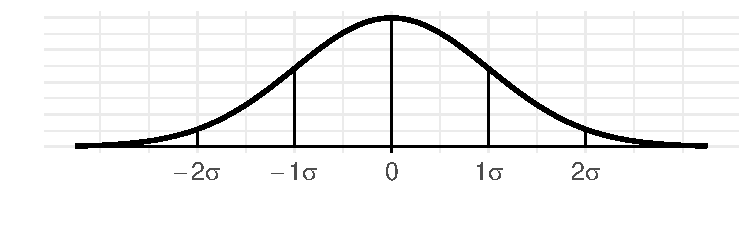
\includegraphics[width=\maxwidth]{img/mc-distribution-02-a-1} 

}







\begin{enumerate}
\item [\textbf{A} \msquare] Die Fläche rechts von $2\sigma$ ist der p-Wert mit $Pr(D|H_0)$ in der obigen Abbildung.
\item [\textbf{B} \msquare] Die Fläche zwischen $-2\sigma$ und $2\sigma$ ist 0.68 und 68\% der Beobachtungen liegen somit zwischen $\bar{y}\pm\sigma$ in der obigen Verteilung.
\item [\textbf{C} \msquare] Dargestellt ist keine Standardnormalverteilung.
\item [\textbf{D} \msquare] Die Fläche unter der Kurve ist 1, wenn die Nullhypothese falsch ist. Wenn die Nullhypothese gilt, dann ist die Fläche $1-\alpha$. Somit ergibt sich auch eine Standardabweichung $\sigma$ mit $\alpha$ gleich 0.05 in beiden Fällen.
\item [\textbf{E} \msquare] Die Fläche zwischen $-1\sigma$ und $1\sigma$ ist 0.68 und 68\% der Beobachtungen liegen somit zwischen $\bar{y}\pm\sigma$ in der obigen Abbildung.
\end{enumerate} 

\section{Aufgabe \hfill (2 Punkte)}

%% --------------------------------------------------------------------
\ifcollection
\begin{flushright}
\tiny\vspace{-2Ex}
\textbf{\examinhaltstart}
\exammodulestatversuch $\;\bullet$
\exammodulebiostat
\vspace{-1Ex}
\end{flushright}
\fi
%% --------------------------------------------------------------------




Die empfohlene Mindestanzahl an Beobachtungen für die Visualisierung mit einem Boxplot sind...



\begin{enumerate}
\item [\textbf{A} \msquare] Die opimale Anzahl ist größer als hundert Beobachtungen, wobei es gerne sehr viel mehr sein können.
\item [\textbf{B} \msquare] Wir sollten eine Beobachtung mindestens pro Gruppe vorliegen haben.
\item [\textbf{C} \msquare] Wir brauchen fünf oder mehr Beobachtungen.
\item [\textbf{D} \msquare] 1 Beobachtung.
\item [\textbf{E} \msquare] Die untere Grenze liegt bei zwei bis fünf Beobachtungen.
\end{enumerate}

\section{Aufgabe \hfill (2 Punkte)}

%% --------------------------------------------------------------------
\ifcollection
\begin{flushright}
\tiny\vspace{-2Ex}
\textbf{\examinhaltstart}
\exammodulestatversuch $\;\bullet$
\exammodulebiostat
\vspace{-1Ex}
\end{flushright}
\fi
%% --------------------------------------------------------------------




In der Statistik müssen wir häufig überprüfen, ob unser Outcome einer bestimmten Verteilung folgt. Meistens überprüfen wir, ob eine
Normalverteilung vorliegt. Folgende drei Abbildungen eigenen sich im Besonderen für die Überprüfung einer Verteilungsannahme an eine Variable.





\begin{enumerate}
\item [\textbf{A} \msquare] Histogramm, Densityplot, Dotplot
\item [\textbf{B} \msquare] Boxplot, Violinplot, Mosaicplot
\item [\textbf{C} \msquare] Violinplot, Scatterplot, Barplot
\item [\textbf{D} \msquare] Barplot, Mosaicplot, Violinplot
\item [\textbf{E} \msquare] Densityplot, Boxplot, Violinplot
\end{enumerate}

\section{Aufgabe \hfill (2 Punkte)}


%% --------------------------------------------------------------------
\ifcollection
\begin{flushright}
\tiny\vspace{-2Ex}
\textbf{\examinhaltstart}
\exammodulestatversuch $\;\bullet$
\exammodulebiostat
\vspace{-1Ex}
\end{flushright}
\fi
%% --------------------------------------------------------------------




Sie wollen eine ANOVA im Anschluss an Ihr Feldexperiment rechnen. Dafür muss Ihr gemessener Endpunkt die Annahme einer Varianzhomogenität genügen. Zur Überprüfung können Sie folgende Visualisierung nutzen. Welche entsprechende Regel zur Abschätzung der Annahme einer Varianzhomogenität kommt zur Anwendung?



\begin{enumerate}
\item [\textbf{A} \msquare] In einer explorativen Datanalyse nutzen wir den Boxplot. Dabei sollte der Median als dicke Linie in der Mitte der Box liegen. Dann können wir von einer Varianzhomogenität ausgehen.
\item [\textbf{B} \msquare] Einen Violinplot. Der Bauch der Violine muss hierbei einen höhren Wert annehmen als der Steg der Violine. Dann kann die Annahme einer Varianzhomogenität angenommen werden.
\item [\textbf{C} \msquare] In einer explorativen Datanalyse nutzen wir den Violinplot. Dabei sollte der Bauch am Rand liegen. Dann können wir von einer Varianzhomogenität ausgehen.
\item [\textbf{D} \msquare] Einen Barplot. Die Mittelwerte müssen alle auf einer Höhe liegen. Die Fehlerbalken haben hier keine Informationen.
\item [\textbf{E} \msquare] Einen Boxplot. Das IQR muss über alle Behandlungen zusammen mit den Whiskers ungefähr gleich aussehen.
\end{enumerate}
\section*{Statistische Testtheorie}  

\section{Aufgabe \hfill (2 Punkte)}

%% --------------------------------------------------------------------
\ifcollection
\begin{flushright}
\tiny\vspace{-2Ex}
\textbf{\examinhaltstart}
\exammodulemathstat $\;\bullet$
\exammodulestat $\;\bullet$
\exammodulestatbbv $\;\bullet$
\exammodulestatversuch $\;\bullet$
\exammodulebiostat
\vspace{-1Ex}
\end{flushright}
\fi
%% --------------------------------------------------------------------




Sie haben den mathematischen Ausdruck $Pr(D|H_0)$ vorliegen, welche Aussage ist richtig?



\begin{enumerate}
\item [\textbf{A} \msquare] Die Wahrscheinlichkeit für die Nullhypothese, wenn die Daten wahr sind.
\item [\textbf{B} \msquare] $Pr(D|H_0)$ ist die Wahrscheinlichkeit nicht die Daten $D$ zu beobachten sondern die Nullhypothese, wenn diese wahr ist.
\item [\textbf{C} \msquare] $Pr(D|H_0)$ ist die Wahrscheinlichkeit der Alternativehypothese und somit $1 - Pr(H_A)$
\item [\textbf{D} \msquare] $Pr(D|H_0)$ beschreibt die Wahrscheinlichkeit die Teststatistik $T_D$ aus den Daten $D$ zu beobachten, wenn die Nullhypothese wahr ist.
\item [\textbf{E} \msquare] $Pr(D|H_0)$ stellt die Wahrscheinlichkeit die Teststatistik $T$ zu beobachten dar, wenn die Nullhypothese falsch ist.
\end{enumerate} 

\section{Aufgabe \hfill (2 Punkte)}

%% --------------------------------------------------------------------
\ifcollection
\begin{flushright}
\tiny\vspace{-2Ex}
\textbf{\examinhaltstart}
\exammodulemathstat $\;\bullet$
\exammodulestat $\;\bullet$
\exammodulestatbbv $\;\bullet$
\exammodulestatversuch $\;\bullet$
\exammodulebiostat
\vspace{-1Ex}
\end{flushright}
\fi
%% --------------------------------------------------------------------




In fast allen wissenschaftlichen Disziplinen liegt der Grenzwert für das Signifikanzniveau $\alpha$ bei 5\%. Wieso wurde dieser Konsens über die Signifikanzschwelle in dieser Form getroffen?



\begin{enumerate}
\item [\textbf{A} \msquare] Da Wissenschaftler eine Schwelle für die statistische Testentscheidung benötigen wurde $\alpha$ in einer großen Konferenz 1945 gewählt. Damit ist $\alpha = 5\%$ eine Kulturkonstante mit einem Rank einer Naturkonstante.
\item [\textbf{B} \msquare] Der Begründer der modernen Statistik, R. Fischer, hat die Grenze simuliert und berechnet. Dadurch ergibt sich dieser optimale Cut-Off.
\item [\textbf{C} \msquare] Im Rahmen eines langen Disputs zwischen Neyman und Fischer wurde $\alpha = 5\%$ festgelegt. Leider werden die Randbedingungen und Voraussetzungen an statistsiche Modelle heute immer wieder ignoriert.
\item [\textbf{D} \msquare] Da Wissenschaftler eine Schwelle für die statistische Testentscheidung benötigen wurde $\alpha$ historisch gewählt. Damit ist $\alpha = 5\%$ eine Kulturkonstante.
\item [\textbf{E} \msquare] Der Wert ergab sich aus einer Auswertung von 1042 wissenschaftlichen Veröffentlichungen zwischen 1914 und 1948. Der Wert $5\%$ wurde in $28\%$ der Veröffentlichungen genutzt. Daher legte man sich auf diese Zahl fest.
\end{enumerate} 

\section{Aufgabe \hfill (2 Punkte)}

%% --------------------------------------------------------------------
\ifcollection
\begin{flushright}
\tiny\vspace{-2Ex}
\textbf{\examinhaltstart}
\exammodulemathstat $\;\bullet$
\exammodulestat $\;\bullet$
\exammodulestatbbv $\;\bullet$
\exammodulestatversuch $\;\bullet$
\exammodulebiostat
\vspace{-1Ex}
\end{flushright}
\fi
%% --------------------------------------------------------------------




Das statistische Testen basiert auf dem Falsifikationsprinzip. Es besagt,



\begin{enumerate}
\item [\textbf{A} \msquare] ... dass ein schlechtes Modell durch das Falsifikationsprinzip durch ein noch schlechteres Modell ersetzt wird. Die Wissenschaft lehnt ab und verifiziert nicht.
\item [\textbf{B} \msquare] ... dass ein minderwertes Modell durch ein minderwertiges Modell ersetzt wird. Es gilt das Verifikationsprinzip nach Karl Popper.
\item [\textbf{C} \msquare] ... dass ein schlechtes Modell durch ein schlechteres Modell ersetzt wird. Die Wissenschaft lehnt ab und verifiziert nicht.
\item [\textbf{D} \msquare] ... dass ein minderwertes Modell durch ein weniger minderwertiges Modell ersetzt wird. Es gilt das Falsifikationsprinzip nach Karl Popper.
\item [\textbf{E} \msquare] ... dass Fehlerterme in statistischen Modellen nicht verifiziert werden können.
\end{enumerate}

\section{Aufgabe \hfill (2 Punkte)}

%% --------------------------------------------------------------------
\ifcollection
\begin{flushright}
\tiny\vspace{-2Ex}
\textbf{\examinhaltstart}
\exammodulemathstat $\;\bullet$
\exammodulestat $\;\bullet$
\exammodulestatbbv $\;\bullet$
\exammodulestatversuch $\;\bullet$
\exammodulebiostat
\vspace{-1Ex}
\end{flushright}
\fi
%% --------------------------------------------------------------------




Betrachten wir die Teststatistik aus einem abstrakteren Blickwinkel. Beim statistischen Testen wird das 	extit{signal} mit dem 	extit{noise} aus den Daten $D$ zu einer Teststatistik $T_D$ verrechnet. Welche der Formel berechnet korrekt die Teststatistik $T_D$?



\begin{enumerate}
\item [\textbf{A} \msquare] Bei der Berechnung der Teststatistik $T_D$ gewichten wir den Effekt $signal$ mit der Varianz $noise$. Wir können verallgemeinert $T_D = signal \cdot noise$ schreiben.
\item [\textbf{B} \msquare] Wir gewichten den Effekt $signal$ mit der Varianz $noise$ und erhalten $T_D = \sfrac{signal}{noise}$.
\item [\textbf{C} \msquare] Bei der Berechnung der Teststatistik $T_D$ gewichten wir den Effekt $signal$ mit der Varianz $noise$. Wir können verallgemeinert $T_D = \sfrac{signal}{noise^2}$ schreiben.
\item [\textbf{D} \msquare] Es gilt $T_D = signal \cdot noise$. Der Effekt $signal$ wird mit der Varianz $noise$ gewichtet.
\item [\textbf{E} \msquare] Es gilt $T_D = \sfrac{signal}{noise}$. Der Effekt $noise$ wird mit der Varianz $signal$ gewichtet.
\end{enumerate}

%% ------------------------------------------------------------

\section{Aufgabe \hfill (2 Punkte)}

%% --------------------------------------------------------------------
\ifcollection
\begin{flushright}
\tiny\vspace{-2Ex}
\textbf{\examinhaltstart}
\exammodulemathstat $\;\bullet$
\exammodulestat $\;\bullet$
\exammodulestatbbv $\;\bullet$
\exammodulestatversuch $\;\bullet$
\exammodulebiostat
\vspace{-1Ex}
\end{flushright}
\fi
%% --------------------------------------------------------------------




Sie haben ein Signifikanzniveau $\alpha$ gleich 5\% vorliegen. Welche Aussage zusammen mit dem $p$-Wert ist richtig?



\begin{enumerate}
\item [\textbf{A} \msquare] Wir vergleichen mit dem $p$-Wert und dem Signifikanzniveau $\alpha$ absolute Werte auf einem Zahlenstrahl und damit den Unterschied der Teststatistiken, wenn die $H_0$ gilt.
\item [\textbf{B} \msquare] Wir schauen, ob der $p$-Wert kleiner ist als das Signifikanzniveau $\alpha$. Wir sprechen von einem signifikanten Ergebnis. Dabei vergleichen wir somit Wahrscheinlichkeiten. Die Wahrscheinlichkeiten werden als Flächen unter der Kurve der Teststaistik dargestellt, wenn die $H_0$ gilt.
\item [\textbf{C} \msquare] Wir vergleichen mit dem $p$-Wert und dem Signifikanzniveau $\alpha$ Wahrscheinlichkeiten und damit die absoluten Werte auf einem Zahlenstrahl, wenn die $H_0$ gilt.
\item [\textbf{D} \msquare] Wir vergleichen die Effekte des $p$-Wertes mit den Effekten der Signifikanzschwelle unter der Annahme der Nullhypothese. Dabei gilt, dass wir die Nullhypothese nur ablehnen können anhand des Falsifikationsprinzips.
\item [\textbf{E} \msquare] Wir machen ein Aussage über die Flächen unter der Kurve der Teststatistik der Hypothese $H_0$ und über die Flächen unter den Kurve der Teststatistik der Hypothese $H_A$. Dabei werden Wahrscheinlichkeiten vergleichen, die durch die Flächen unter der Kurve der beiden Testverteilungen repräsentiert werden.
\end{enumerate}

\section{Aufgabe \hfill (2 Punkte)}

%% --------------------------------------------------------------------
\ifcollection
\begin{flushright}
\tiny\vspace{-2Ex}
\textbf{\examinhaltstart}
\exammodulemathstat $\;\bullet$
\exammodulestat $\;\bullet$
\exammodulestatbbv $\;\bullet$
\exammodulestatversuch $\;\bullet$
\exammodulebiostat
\vspace{-1Ex}
\end{flushright}
\fi
%% --------------------------------------------------------------------




Die Ergebnisse der einer statistischen Analyse können in die Analogie einer Wettervorhersage gebracht werden. Welche Analogie für die Ergebnisse eines statistischen Tests trifft am besten zu?



\begin{enumerate}
\item [\textbf{A} \msquare] In der Analogie der Regenwahrscheinlichkeit in einem bestimmten Gebiet: ein statistischer Test gibt die Wahrscheinlichkeit für ein Ereignis in einem Experiment mit den Daten $D$ wieder und lässt sich kaum verallgemeinern.
\item [\textbf{B} \msquare] In der Analogie der Maximaltemperatur: Was ist der maximale Unterschied zwischen zwei Gruppen. Wir erhalten hier eine Aussage über die Spannweite und den maximalen Effekt.
\item [\textbf{C} \msquare] In der Analogie der Durchschnittstemperatur: Wie oft tritt ein Effekt durchschnittlich ein? Wir erhalten eine Wahrscheinlichkeit für die Effekte. Zum Beispiel, wie hoch ist die Wahrscheinlichkeit für einen Mittelwert als Durchschnitt.
\item [\textbf{D} \msquare] In der Analogie des Niederschlags oder Regenmenge: ein statistischer Test gibt die Stärke eines Effektes wieder. Zum Beispiel, wie hoch ist der Mittelwertsunterschied.
\item [\textbf{E} \msquare] In der Analogie der Wahrscheinlichkeit für Regen: ein statistischer Test erlaubt die Wahrscheinlichkeit für ein Ereignis abzuschätzen. Die Stärke des Effektes können wir nicht bestimmen.
\end{enumerate}

\section{Aufgabe \hfill (2 Punkte)}

%% --------------------------------------------------------------------
\ifcollection
\begin{flushright}
\tiny\vspace{-2Ex}
\textbf{\examinhaltstart}
\exammodulemathstat $\;\bullet$
\exammodulestat $\;\bullet$
\exammodulestatbbv $\;\bullet$
\exammodulestatversuch $\;\bullet$
\exammodulebiostat
\vspace{-1Ex}
\end{flushright}
\fi
%% --------------------------------------------------------------------




In Ihrer Forschungsarbeit wollen Sie eine Aussage über \underline{ein} untersuchtes Individuum treffen. Dazu nutzen Sie einen statistischen Test. Erhalten Sie eine valide Aussage aus einem statistischen Test?



\begin{enumerate}
\item [\textbf{A} \msquare] Nein, wir können \underline{ein} untersuchtes Individuum nicht mit einer statistischen Analyse auswerten. Wir erhalten keine Aussage zum Individuum.
\item [\textbf{B} \msquare] Weder eine Ausssage über die Population noch über das Individuum ist mit einem statistischen Test möglich. Wir erhalten eine Aussage über ein Experiment.
\item [\textbf{C} \msquare] Nein, wir können \underline{ein} untersuchtes Individuum nicht mit einer ANOVA auswerten. Wir erhalten keine Aussage zum Individuum. Wir können aber den Test adjustieren und so die Auswertung ermöglichen.
\item [\textbf{D} \msquare] Nein, wir erhalten nur eine Aussage zu zwei Individuen. Ein statistischer Test liefert Informationen zu einem Individuum im Vergleich zu einem anderen Individuum.
\item [\textbf{E} \msquare] Ja, wir können \underline{ein} untersuchtes Individuum mit einem statistischen Test auswerten. Wir erhalten eine Aussage zum Individuum.
\end{enumerate}

\section{Aufgabe \hfill (2 Punkte)}

%% --------------------------------------------------------------------
\ifcollection
\begin{flushright}
\tiny\vspace{-2Ex}
\textbf{\examinhaltstart}
\exammodulemathstat $\;\bullet$
\exammodulestat $\;\bullet$
\exammodulestatbbv $\;\bullet$
\exammodulestatversuch $\;\bullet$
\exammodulebiostat
\vspace{-1Ex}
\end{flushright}
\fi
%% --------------------------------------------------------------------




Welche Aussage über den Effekt eines statistischen Tests ist richtig?



\begin{enumerate}
\item [\textbf{A} \msquare] Der Effekt eines statistischen Tests beschreibt die biologisch interpretierbare Ausgabe eines Tests. Moderen Algorithmen liefern keine Effekte mehr sondern nur noch bedingte Wahrscheinlichkeiten. Der Effekt spielt in der modernen Statistik keine Rollen mehr.
\item [\textbf{B} \msquare] Der Forschende muss am Anfang wissen, ob das Eregbnis eines Experiments relevant für seine Forschung ist. Dafür kann der Effekt eines statistischen Tests genutzt werden oder auch der Prähoc-Test. Damit beschreibt der Effekt den biologischen interpretierbaren Teil eines Experimnts vor der Durchführung. Zum Beispiel der Unterschied zwischen zwei Mittelwerten.
\item [\textbf{C} \msquare] Der Forschende muss am Ende wissen, ob das Eregbnis eines Experiments relevant für seine Forschung ist. Dafür kann der Effekt eines statistischen Tests genutzt werden. Damit beschreibt der Effekt den biologischen interpretierbaren Teil einer Ausgabe eines Tests. Zum Beispiel der Unterschied zwischen zwei Anteilen.
\item [\textbf{D} \msquare] Der Effekt eines statistischen Tests beschreibt den Output oder die Wiedergabe eines Tests in einem Computer.
\item [\textbf{E} \msquare] Durch den Effekt erfahren wir die statistische interpretierbare Ausgabe eines statistischen Tests. Zum Beispiel das $\eta^2$ aus einer ANOVA. Damit können wir die Signifikanz direkt mit dem Effekt verbinden. Am Ende muss der Forschende aber entscheiden, ob der Effekt entsprechend seinen Erwartungen als bedeutet zu bewerten ist.
\end{enumerate}

\section{Aufgabe \hfill (2 Punkte)}

%% --------------------------------------------------------------------
\ifcollection
\begin{flushright}
\tiny\vspace{-2Ex}
\textbf{\examinhaltstart}
\exammodulemathstat $\;\bullet$
\exammodulestat $\;\bullet$
\exammodulestatbbv $\;\bullet$
\exammodulestatversuch $\;\bullet$
\exammodulebiostat
\vspace{-1Ex}
\end{flushright}
\fi
%% --------------------------------------------------------------------



Roland Fischer entwickelte Anfang des letzten Jahrhunderts als Grundlage für das experimentelle Design in der Statistik die Randomisierung. Warum ist die Randomisierung für die Entscheidung anhand einer statistischen Auswertung so wichtig?



\begin{enumerate}
\item [\textbf{A} \msquare] Randomisierung war bis 1952 bedeutend, wurde dann aber in Folge besserer Rechnerleistung nicht mehr verwendet. Aktuelle Statistik nutzt keine Randomisierung mehr.
\item [\textbf{B} \msquare] Randomisierung erlaubt erst die Varianzen zu schätzen. Ohne eine Randomisierung ist die Berechnung von Mittelwerten und Varianzen nicht möglich. Dadurch lässt sich erst ein Experiment auswerten.
\item [\textbf{C} \msquare] Randomisierung erlaubt erst die Mittelwerte zu schätzen. Ohne Randomisierung keine Mittelwerte. Ohne Mittelwerte keine Varianz und somit auch kein statistischer Test.
\item [\textbf{D} \msquare] Durch eine Randomisierung können wir von Strukturgleichheit zwischen der Stichprobe und der Grundgesamtheit ausgehen.
\item [\textbf{E} \msquare] Durch eine Randomisierung können wir nicht von Strukturgleichheit zwischen der Stichprobe und der Grundgesamtheit ausgehen.
\end{enumerate}

\section{Aufgabe \hfill (2 Punkte)}

%% --------------------------------------------------------------------
\ifcollection
\begin{flushright}
\tiny\vspace{-2Ex}
\textbf{\examinhaltstart}
\exammodulemathstat $\;\bullet$
\exammodulestat $\;\bullet$
\exammodulestatbbv $\;\bullet$
\exammodulestatversuch $\;\bullet$
\exammodulebiostat
\vspace{-1Ex}
\end{flushright}
\fi
%% --------------------------------------------------------------------




Wenn Sie im Allgemeinen einen statistischen Test rechnen, dann kommen Sie um eine statistische Hypothese $H$ nicht herum. Welche Aussage über statistische Hypothesen ist richtig?



\begin{enumerate}
\item [\textbf{A} \msquare] Es gibt ein Hypothesenset bestehend aus $k$ Hypothesen. Meistens wird die Nullhypothese $H_0$ und die Alternativhypothese $H_A$ verwendet. Wegen des Falsifikationsprinzips ist es wichtig, die bekannte falsche und unbekannte richtige Hypothese mit in das Set zu nehmen.
\item [\textbf{B} \msquare] Mit der Nullhypothese $H_A$ und der Alternativehypothese $H_0$ gibt es zwei Hypothesen, die aber selten genutzt werden.
\item [\textbf{C} \msquare] Mit der Nullhypothese $H_0$ und der Alternativehypothese $H_A$ oder $H_1$ gibt es zwei Hypothesen.
\item [\textbf{D} \msquare] Es gibt - bedingt durch das das Falsifikationsprinzip - ein Set von $k$ Nullhypothesen, die iterative gegen $k-1$ Alternativhypothesen getestet werden.
\item [\textbf{E} \msquare] Ein statistisches Hypothesenpaare gibt es. Zum einen die Nullhypothese und zum anderen die Alternativehypothese. Es ist aber nur notwendig die Alternative anzugeben, da die Nullhypothese nicht beim Testen benötigt wird.
\end{enumerate}

\section{Aufgabe \hfill (2 Punkte)}

%% --------------------------------------------------------------------
\ifcollection
\begin{flushright}
\tiny\vspace{-2Ex}
\textbf{\examinhaltstart}
\exammodulemathstat $\;\bullet$
\exammodulestat $\;\bullet$
\exammodulestatbbv $\;\bullet$
\exammodulestatversuch $\;\bullet$
\exammodulebiostat
\vspace{-1Ex}
\end{flushright}
\fi
%% --------------------------------------------------------------------




In der Theorie zur statistischen Testentscheidung kann folgende Aussage
in welche richtige Analogie gesetzt werden?

\begin{center}
\textit{$H_0$ ablehnen obwohl die $H_0$ gilt}
\end{center}



\begin{enumerate}
\item [\textbf{A} \msquare] Dem $\beta$-Fehler mit der Analogie eines Rauchmelders: \textit{Fire without alarm}.
\item [\textbf{B} \msquare] In die Analogie eines Rauchmelders: \textit{Alarm without fire}, dem $\alpha$-Fehler.
\item [\textbf{C} \msquare] In die Analogie eines Feuerwehrautos: \textit{Car without noise}.
\item [\textbf{D} \msquare] In die Analogie eines brennenden Hauses ohne Rauchmelder: \textit{House without noise}.
\item [\textbf{E} \msquare] In die Analogie eines Rauchmelders: \textit{Alarm with fire}.
\end{enumerate}

\section{Aufgabe \hfill (2 Punkte)}

%% --------------------------------------------------------------------
\ifcollection
\begin{flushright}
\tiny\vspace{-2Ex}
\textbf{\examinhaltstart}
\exammodulestat $\;\bullet$
\exammodulestatbbv $\;\bullet$
\exammodulestatversuch $\;\bullet$
\exammodulebiostat
\vspace{-1Ex}
\end{flushright}
\fi
%% --------------------------------------------------------------------




Sie sollen in Ihrer Abschlussarbeit die Relevanz und die Signifikanz in einer statistischen Maßzahl vereinen. Welche Aussage ist richtig?



\begin{enumerate}
\item [\textbf{A} \msquare] Der p-Wert. Durch den Vergleich mit $\alpha$ lässt sich über die Signifikanz entscheiden und der $\beta$-Fehler erlaubt über die Power eine Einschätzung der Relevanz.
\item [\textbf{B} \msquare] Die Teststatistik. Durch den Vergleich von $T_c$ zu $T_k$ ist es m{"o}glich die $H_0$ abzulehnen. Die Relevanz ergibt sich aus der Fläche rechts vom dem $T_c$-Wert.
\item [\textbf{C} \msquare] Einem Konfidenzintervall. Das Konfidenzinterval bringt durch eine Visualisierung und zwei Intervallgrenzen die Möglichkeit mit, eine Relevanzschwelle neben der definierten Signifikanzschwelle zu definieren.
\item [\textbf{D} \msquare] Einem Konfidenzintervall. Das Konfidenzinterval bringt durch eine Visualisierung und drei Intervallgrenzen die Möglichkeit mit, eine Relevanzschwelle neben der Signifikanzschwelle und der $\alpha$-Schwelle zu definieren.
\item [\textbf{E} \msquare] Über das Konfidenzintervall. Das Konfidenzinterval inkludiert eine Entscheidung über die Relevanz und zusätzlich kann über die Visualizierung des Konfidenzintervals eine Signifikanzschwelle vom Forschenden definiert werden.
\end{enumerate}

\section{Aufgabe \hfill (2 Punkte)}

%% --------------------------------------------------------------------
\ifcollection
\begin{flushright}
\tiny\vspace{-2Ex}
\textbf{\examinhaltstart}
\exammodulestatversuch $\;\bullet$
\exammodulebiostat
\vspace{-1Ex}
\end{flushright}
\fi
%% --------------------------------------------------------------------




Sie werten in Ihrer Abschlussarbeit einen sehr großen Datensatz aus einer öffentlichen Datenbank aus. Nun stellen Sie fest, dass Sie ein Problem mit der Bewertung Ihrer Ergbnisse anhand der Signifikanz bekommen. Wie Sie herausfinden, scheint dies ein häufiges Problem in der Bio Data Science zu sein. Welche Aussage ist richtig?




\begin{enumerate}
\item [\textbf{A} \msquare] Aktuell werden zu grosse Datensätze für die gänigige Statistik gemessen. Daher wendet man maschinelle Lernverfahren für kausale Modelle an. Hier ist die Relevanz gleich Signifikanz.
\item [\textbf{B} \msquare] Riesige Datensätz haben mehr Fallzahl was zur $\alpha$-Inflation führt. Durch eine Adjustoerung kann dem Problem entgegengewirkt werden.
\item [\textbf{C} \msquare] Eine erhöhte Fallzahl führt automatisch zu mehr signifikanten Ergebnissen auch wenn der Effekt klein ist und damit nicht relevant. Dadurch sind die Informationen zur Signifikanz in riesigen Datensätzen schwer zu verwerten, da fast alle Vergleiche signifikant sind.
\item [\textbf{D} \msquare] Relevanz und Signifikanz haben nichts miteinander zu tun. Daher gibt es auch keinen Zusammenhang zwischen hoher Fahlzahl (n > 10000) und einem signifikanten Test. Ein Effekt ist immer relevant und somit signifikant.
\item [\textbf{E} \msquare] Big Data ist ein Problem der parametrischen Statistik. Parameter lassen sich nur auf kleinen Datensätzen berechnen, da es sich sonst nicht mehr um eine Stichprobe im engen Sinne der Statistik handelt.
\end{enumerate}

\section{Aufgabe \hfill (2 Punkte)}

%% --------------------------------------------------------------------
\ifcollection
\begin{flushright}
\tiny\vspace{-2Ex}
\textbf{\examinhaltstart}
\exammodulestatversuch $\;\bullet$
\exammodulebiostat
\vspace{-1Ex}
\end{flushright}
\fi
%% --------------------------------------------------------------------




Im Rahmen Ihrer Abschlussarbeit werten Sie ein Experiment mit Ferkel aus. Es geht um die Leistungssteigerung der Ferkelproduktion. Sie messen jeweils die Gewichtszunahme der Ferkel. Die Ferkel einer Muttersau sind dabei...



\begin{enumerate}
\item [\textbf{A} \msquare] Untereinander unabhängig. Sollten die Mütter verwandt sein, so ist die Varianzstruktur ähnlich und muss modelliert werden.
\item [\textbf{B} \msquare] Untereinander stark korreliert. Die Ferkel sind von einer Mutter und sommit miteinander korreliert. Dies wird in der Statistik jedoch meist nicht modelliert.
\item [\textbf{C} \msquare] Die Ferkel stammen von der gleichen Sau und sind somit untereinander abhängig.
\item [\textbf{D} \msquare] Abhängig von der Stallanlage und des Experiments können die Ferkel abhängig oder unabhängig sein. Allgmein gilt, dass Ferkel von unterschiedlichen Sauen näher miteinander verwandt sind als Ferkel von gleichen Sauen. Das Fisher-Axiom.
\item [\textbf{E} \msquare] Untereinander unabhängig. Die Ferkel sind eigenständig und benötigen keine zusätzliche Behandlung.
\end{enumerate}

\section{Aufgabe \hfill (2 Punkte)}

%% --------------------------------------------------------------------
\ifcollection
\begin{flushright}
\tiny\vspace{-2Ex}
\textbf{\examinhaltstart}
\exammodulestatversuch $\;\bullet$
\exammodulebiostat
\vspace{-1Ex}
\end{flushright}
\fi
%% --------------------------------------------------------------------






Sie rechnen einen statistischen Test und wollen anhand des 95\%-Konfidenzintervalls eine Entscheidung gegen die Nullhypothese treffen. Welche Aussage ist richtig?





\begin{enumerate}
\item [\textbf{A} \msquare] Ist in dem 95\%-Konfidenzintervall nicht die Null enthalten dann wird die Nullhypothese $H_0$ abgelehnt.
\item [\textbf{B} \msquare] Ist $T_{D}$ höher als der kritische Wert $T_{\alpha = 5\%}$ dann wird die Nullhypothese $H_0$ abgelehnt.
\item [\textbf{C} \msquare] Das Signifikanzniveau $\alpha$ ist gleich $5\%$ und das berechnete Intervall muss gleich\textit{er} als das Signifikanzniveau sein.
\item [\textbf{D} \msquare] Anhand des 95\%-Konfidenzintervalls lässt sich wie folgt eine Entscheidung treffen. Liegt der Wert über oder gleich dem Signifikanzniveau $\alpha$ dann kann die Nullhypothese abgelehnt werden.
\item [\textbf{E} \msquare] Das Signifikanzniveau $\alpha$ ist gleich $5\%$. $Pr(D|H_0)$ muss kleiner sein als das Signifikanzniveau.
\end{enumerate}

\section{Aufgabe \hfill (2 Punkte)}

%% --------------------------------------------------------------------
\ifcollection
\begin{flushright}
\tiny\vspace{-2Ex}
\textbf{\examinhaltstart}
\exammodulebiostat
\vspace{-1Ex}
\end{flushright}
\fi
%% --------------------------------------------------------------------




Sie haben die \textit{Power} berechnet. Was sagt Ihnen dieser statistische Begriff aus?



\begin{enumerate}
\item [\textbf{A} \msquare] Alle statistischen Tests sind so konstruiert, dass die $H_A$ mit 80\% \textit{bewiesen wird}. Die Power ist $1-\beta$ mit $\beta$ gleich 20\% gesetzt.
\item [\textbf{B} \msquare] Die Power $1-\beta$ wird auf 80\% gesetzt. Damit liegt die Wahrscheinlichkeit für die $H_0$ bei 20\%.
\item [\textbf{C} \msquare] Die Power ist nicht in der aktuellen Testthorie mehr vertreten. Wir rechnen nur noch mit dem Fehler 1. Art.
\item [\textbf{D} \msquare] Es gilt $\alpha + \beta = 1$ und somit liegt $\beta$ meist bei 95\%.
\item [\textbf{E} \msquare] Alle statistischen Tests sind so konstruiert, dass die $H_A$ mit 20\% \textit{bewiesen wird}. Die Power ist $1-\beta$ mit $\beta$ gleich 80\% gesetzt.
\end{enumerate}
\section*{Statistische Tests für Gruppenvergleiche} 

\section{Aufgabe \hfill (2 Punkte)}

%% --------------------------------------------------------------------
\ifcollection
\begin{flushright}
\tiny\vspace{-2Ex}
\textbf{\examinhaltstart}
\exammodulemathstat $\;\bullet$
\exammodulestat $\;\bullet$
\exammodulestatbbv 
\vspace{-1Ex}
\end{flushright}
\fi
%% --------------------------------------------------------------------




In Ihrer Abschlussarbeit rechnen Sie einen Student t-Test. Welche Aussage ist auch für den Welch t-Test richtig?



\begin{enumerate}
\item [\textbf{A} \msquare] Der t-Test testet generell zu einem erhöhten $\alpha$-Niveau von 20\%.
\item [\textbf{B} \msquare] Der t-Test vergleicht die Varianzen von mindestens zwei oder mehr Gruppen
\item [\textbf{C} \msquare] Der t-Test vergleicht zwei Gruppen indem die Mittelwerte miteinander verglichen werden.
\item [\textbf{D} \msquare] Der t-Test vergleicht zwei oder mehr Gruppen indem die Mittelwerte miteinander verglichen werden.
\item [\textbf{E} \msquare] Der t-Test vergleicht die Mittelwerte von zwei Gruppen unter der strikten Annahme von Varianzhomogenität. Sollte keine Varianzhomogenität vorliegen, so gibt es keine Möglichkeit den t-Test in einer Variante anzuwenden.
\end{enumerate}

\section{Aufgabe \hfill (2 Punkte)}

%% --------------------------------------------------------------------
\ifcollection
\begin{flushright}
\tiny\vspace{-2Ex}
\textbf{\examinhaltstart}
\exammodulestatversuch $\;\bullet$
\exammodulebiostat
\vspace{-1Ex}
\end{flushright}
\fi
%% --------------------------------------------------------------------





In Ihrer Abschlussarbeit betrachten Sie die Effekte von einer Behandlung vor und nach der Gabe eines Vitamins. Sie müssen einen gepaarten t-Test rechnen. Welche Aussage ist richtig?



\begin{enumerate}
\item [\textbf{A} \msquare] Der gepaarte t-Test wird gerechnet, wenn die Beobachtungen abhängig voneinander sind. Wir messen jede Beobachtung nur einmal und berechnen dann die Differenz zu dem Mittel der anderen Beobachtungen.
\item [\textbf{B} \msquare] Der gepaarte t-Test nutzt die Varianz der Beobachtungen jeweils paarweise und bildet dafür eine verbundene Stichprobe. Dieser Datensatz $d$ dient dann zur Differenzbildung.
\item [\textbf{C} \msquare] Abhängige Beobachtungen müssen gesondert in einem gepaarten t-Test modelliert werden. Wenn wiederholt an dem gleichen Tier oder Pflanze gemessen wird, dann bilden wir den Quotienten zwischen den beiden Zeitpunkten. Auf den Quotienten rechnen wir den gepaarten t-Test.
\item [\textbf{D} \msquare] Abhängige Beobachtungen müssen gesondert in einem gepaarten t-Test modelliert werden. Wenn wiederholt an dem gleichen Tier oder Pflanze gemessen wird, dann bilden wir die Differenz zwischen den beiden Zeitpunkten. Auf den Differenzen rechnen wir den gepaarten t-Test.
\item [\textbf{E} \msquare] Wenn die Beobachtungen unabhängig voneinander sind, rechnen wir einen gepaarten t-Test. Messen wir wiederholt an dem gleichen Tier oder Pflanze dann bilden wir das Produkt zwischen den zwei Messpunkten.
\end{enumerate}

\section{Aufgabe \hfill (2 Punkte)}

%% --------------------------------------------------------------------
\ifcollection
\begin{flushright}
\tiny\vspace{-2Ex}
\textbf{\examinhaltstart}
\exammodulemathstat $\;\bullet$
\exammodulestat $\;\bullet$
\exammodulestat $\;\bullet$
\exammodulestatbbv $\;\bullet$
\exammodulestatversuch $\;\bullet$
\exammodulebiostat
\vspace{-1Ex}
\end{flushright}
\fi
%% --------------------------------------------------------------------




Die folgende Abbildung enthält die Daten aus einer Studie zur Bewertung der Wirkung des Mikronährstoff Eisen auf den Ertrag in t/ha von Weizen im Vergleich zu einer Kontrolle. Der Versuch wurde in 8 Parzellen pro Gruppe durchgeführt. Welche Aussage im Bezug auf eine statistische Auswertung ist richtig?



{\centering 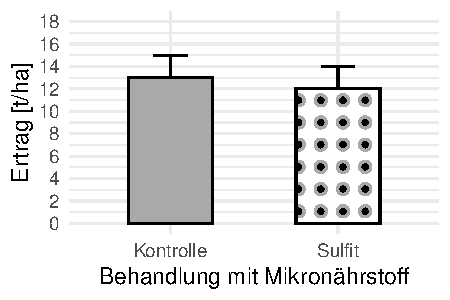
\includegraphics[width=\maxwidth]{img/mc-testing-ttest-02-1} 

}







\begin{enumerate}
\item [\textbf{A} \msquare] Es liegt ein signifikanter Unterschied vor. Der Effekt liegt bei 0.1.
\item [\textbf{B} \msquare] Nach Betrachtung des Barplots liegt kein signifikanter Unterschied vor. Der Effekt kann nicht bei einem t-Test aus Barplots bestimmt werden.
\item [\textbf{C} \msquare] Es liegt ein signifikanter Unterschied vor. Der Effekt liegt bei 1.
\item [\textbf{D} \msquare] Nach Betrachtung des Barplots liegt kein signifikanter Unterschied vor. Der Effekt liegt bei 1.
\item [\textbf{E} \msquare] Die Barplots deuten auf einen signifikanten Unterschied. Der Effekt liegt vermutlich bei 1. Wir müssen aber einen Posthoc-Test rechnen um den Effekt wirklich bestimmen zu können.
\end{enumerate}

\section{Aufgabe \hfill (2 Punkte)}

%% --------------------------------------------------------------------
\ifcollection
\begin{flushright}
\tiny\vspace{-2Ex}
\textbf{\examinhaltstart}
\exammodulestatversuch $\;\bullet$
\exammodulebiostat
\vspace{-1Ex}
\end{flushright}
\fi
%% --------------------------------------------------------------------




In Ihrer Abschlussarbeit passen die Ergebnisse einer ANOVA und eines multiplen Vergleiches nicht zusammen. Nach einem Experiment mit vier Maissorten ergibt eine ANOVA ($p = 0.045$). Sie führen anschließend die paarweisen t-Tests für alle Vergleiche durch. Nach der Adjustierung für multiples Testen ist kein p-Wert unter der $\alpha$-Schwelle. Sie schauen sich auch die rohen, unadjustierten p-Werte an und finden hier als niedrigsten p-Wert $p_{3-2} = 0.053$. Welche Aussage ist richtig?




\begin{enumerate}
\item [\textbf{A} \msquare] Die ANOVA testet auf der gesamten Fallzahl. Es wäre besser die ANOVA auf der gleichen Fallzahl wie die einzelnen t-Tests zu rechnen.
\item [\textbf{B} \msquare] Der Fehler liegt in den t-Tests. Wenn eine ANOVA signifikant ist, dann muss zwangsweise auch ein t-Test signifikant sein.
\item [\textbf{C} \msquare] Hier kommt der Effekt der stiegenden Fallzahl auf die Anzahl an signifikante Ergebnisse zu tragen. Da die ANOVA auf mehr Fallzahl testet als die einzelnen paarweisen t-Tests, kann die ANOVA leichter einen signifikanten Unterscheid nachweisen. Die p-Werte sind immer etwas kleiner als bei den t-Tests.
\item [\textbf{D} \msquare] Hier kommt der Effekt der stiegenden Fallzahl auf die Anzahl an signifikante Ergebnisse zu tragen. Da die ANOVA auf weniger Fallzahl testet als die paarweisen t-Tests, kann die ANOVA schwerer einen signifikanten Unterscheid nachweisen.
\item [\textbf{E} \msquare] Das ist kein Wunder. Die ANOVA testet nicht auf der gesamten Fallzahl und die paarweisen t-Tests gewinnen immer eine oder mehr Gruppen als Fallzahl dazu. Mit steigender Fallzahl sind mehr signifikante Unterschiede zu erwarten. Die p-Werte unterscheiden sich numerisch auch kaum.
\end{enumerate}
\section*{ANOVA}

\section{Aufgabe \hfill (2 Punkte)}

%% --------------------------------------------------------------------
\ifcollection
\begin{flushright}
\tiny\vspace{-2Ex}
\textbf{\examinhaltstart}
\exammodulemathstat $\;\bullet$
\exammodulestat $\;\bullet$
\exammodulestatbbv $\;\bullet$
\exammodulestatversuch $\;\bullet$
\exammodulebiostat
\vspace{-1Ex}
\end{flushright}
\fi
%% --------------------------------------------------------------------






Nach der Berechnung einer einfaktoriellen ANOVA ergibt sich ein $\eta^2 = 0.31$. Welche Aussage ist richtig?



\begin{enumerate}
\item [\textbf{A} \msquare] Das $\eta^2$ beschreibt den Anteil der Varianz, der von den Behandlungsbedingungen erklärt wird.
\item [\textbf{B} \msquare] Das $\eta^2$ beschreibt den Anteil der globalen Varianz, der von den Umweltbedingungen erklärt wird.
\item [\textbf{C} \msquare] Das $\eta^2$ ist die Korrelation der ANOVA. Mit der Ausnahme, dass $\eta^2 = 0$ der beste Wert ist.
\item [\textbf{D} \msquare] Der Anteil der Varianz, der von den Behandlungsbedingungen erklärt wird, wird durch das $1-\eta^2$ beschrieben.
\item [\textbf{E} \msquare] Das $\eta^2$ ist ein Wert für die Güte der ANOVA. Je kleiner desto besser. Ein $\eta^2$ von 0 bedeutet ein perfektes Modell mit keiner Abweichung. Die Varianz ist null.
\end{enumerate}

\section{Aufgabe \hfill (2 Punkte)}

%% --------------------------------------------------------------------
\ifcollection
\begin{flushright}
\tiny\vspace{-2Ex}
\textbf{\examinhaltstart}
\exammodulemathstat $\;\bullet$
\exammodulestat $\;\bullet$
\exammodulestatbbv $\;\bullet$
\exammodulestatversuch $\;\bullet$
\exammodulebiostat
\vspace{-1Ex}
\end{flushright}
\fi
%% --------------------------------------------------------------------







Nach einem Feldexperiment erhalten Sie ein $\eta^2 = 0.23$. aus Ihrer einfaktoriellen ANOVA. Sie haben sich den Chlorophyllgehalt in Kartoffel angeschaut und wollen nun das Ergebnis anhand des $\eta^2$ bewerten. Welche Aussage ist richtig?



\begin{enumerate}
\item [\textbf{A} \msquare] Mit dem $\eta^2$ lässt sich auf die Qualität der Randomisierung und damit der Strukturgleichheit zwischen der Grundgesamtheit und der Stichprobe schließen. Es gilt dabei die Regel, dass ein $\eta^2$-Wert von 1 zu bevorzugen ist.
\item [\textbf{B} \msquare] Es werden 23\% der Varianz durch die Behandlung erklärt. Das $\eta^2$ beschreibt den Anteil der Varianz, der von den unterschiedlichen Behandlungsbedingungen erklärt wird.
\item [\textbf{C} \msquare] Es werden 23\% der Varianz durch den Versuch erklärt. Das $\eta^2$ beschreibt den Anteil der Varianz, der durch Fehler in der Versuchsdurchführung entsteht.
\item [\textbf{D} \msquare] Das $\eta^2$ beschreibt den Anteil der Varianz, der von den Umweltbedingungen erklärt wird. Daher werden 23\% der Varianz durch die Umweltbedingungen erklärt. Der Anteil der Varianz durch die Behandlungsgruppen ist dann 77\%.
\item [\textbf{E} \msquare] Es werden 77\% der Varianz durch die Behandlung erklärt. Das $\eta^2$ beschreibt den Anteil der Varianz, der von den unterschiedlichen Behandlungsbedingungen nicht erklärt wird.
\end{enumerate}

\section{Aufgabe \hfill (2 Punkte)}

%% --------------------------------------------------------------------
\ifcollection
\begin{flushright}
\tiny\vspace{-2Ex}
\textbf{\examinhaltstart}
\exammodulemathstat $\;\bullet$
\exammodulestat $\;\bullet$
\exammodulestatbbv $\;\bullet$
\exammodulestatversuch $\;\bullet$
\exammodulebiostat
\vspace{-1Ex}
\end{flushright}
\fi
%% --------------------------------------------------------------------




Die einfaktorielle ANOVA ist ein Standardverfahren in der agrawissenschaftlichen Forschung wenn es um den Vergleich von Behandlungsgruppen geht. Welche der folgenden Aussage zu der Berechnung der Teststatistik der einfaktoriellen ANOVA ist richtig?



\begin{enumerate}
\item [\textbf{A} \msquare] Die ANOVA berechnet die T-Statistik indem den Mittelwertsunterschied der Gruppen simultan durch die Standardabweichung der Gruppen teilt. Wenn die T-Statistik h{"o}her als 1.96 ist, kann die Nullhypothese abgelehnt werden.
\item [\textbf{B} \msquare] Die ANOVA berechnet die T-Statistik aus der Multiplikation der MS Behandlung mit der MS der Fehler. Wenn die F-Statistik genau 0 ist, kann die Nullhypothese nicht abgelehnt werden.
\item [\textbf{C} \msquare] Wenn die F-Statistik höher ist als der kritische Wert kann die Nullhypothese nicht abgelehnt werden. Die F-Statistik ist die Differenz der MS der Behandlung durch die MS des Fehlers.
\item [\textbf{D} \msquare] Die ANOVA berechnt die F-Statistik aus den SS Behandlung geteilt durch die SS Fehler.
\item [\textbf{E} \msquare] Die ANOVA berechnet die F-Statistik indem die MS der Behandlung durch die MS des Fehlers geteilt werden. Wenn die F-Statistik sich der 0 ann{"a}hert kann die Nullhypothese nicht abgelehnt werden.
\end{enumerate}

\section{Aufgabe \hfill (2 Punkte)}

%% --------------------------------------------------------------------
\ifcollection
\begin{flushright}
\tiny\vspace{-2Ex}
\textbf{\examinhaltstart}
\exammodulemathstat $\;\bullet$
\exammodulestat $\;\bullet$
\exammodulestatbbv $\;\bullet$
\exammodulestatversuch $\;\bullet$
\exammodulebiostat
\vspace{-1Ex}
\end{flushright}
\fi
%% --------------------------------------------------------------------




Wenn Sie mehr als zwei Gruppen als Behandlungen vorliegen haben, dann kann ein einfacher t-Test nicht für den globalen Vergleich genutzt werden. Sie entscheiden sich für eine ANOVA in \Rlogo. Die ANOVA analysiert dabei...



\begin{enumerate}
\item [\textbf{A} \msquare] ... den Unterschied zwischen der Varianz über alle Behandlungsgruppen oder der Varianz aus verschiedenen Behandlungsguppen. Wenn die ANOVA signifikant ist, muss sich zwischen einem der beiden Varianzquellen entschieden werden.
\item [\textbf{B} \msquare] ... den Unterschied zwischen der F-Statistik anhand der Varianz der Gruppen. Wenn die F-Statistik exakt 0 ist, kann die Nullhypothese abgelehnt werden.
\item [\textbf{C} \msquare] ... den Unterschied zwischen der Varianz über alle Behandlungsgruppen und der Varianz aus verschiedenen Behandlungsguppen. Wenn die ANOVA signifikant ist, muss ein Posthoc-Test angeschlossen werden.
\item [\textbf{D} \msquare] ... den Unterschied zwischen zwei paarweisen Mittelwerten aus verschiedenen Behandlungsguppen. Wenn die signifikant ist, ist daher bekannt welcher Vergleich konkret unterschiedlich ist.
\item [\textbf{E} \msquare] ... den Unterschied zwischen der Varianz in den verschiedenen Behandlungsguppen und der Varianz in einer der Behandlungsgruppen. Wenn die ANOVA signifikant ist, muss über einen Posthoc-Test nachgedacht werden um den signifikanten Unterschied in einer der Gruppen exakt zu bestimmen.
\end{enumerate}

\section{Aufgabe \hfill (2 Punkte)}

%% --------------------------------------------------------------------
\ifcollection
\begin{flushright}
\tiny\vspace{-2Ex}
\textbf{\examinhaltstart}
\exammodulestatversuch $\;\bullet$
\exammodulebiostat
\vspace{-1Ex}
\end{flushright}
\fi
%% --------------------------------------------------------------------




Ein Versuch wurde an 50 Tieren durchgeführt, wobei jedes Tier eine von drei Vitamin-C-Dosen (0.5, 1 und 1.5 mg/Tag) über eine von zwei Verabreichungsmethoden erhielt. Die folgende Abbildung enthält die Daten aus diesem Versuch zur Bewertung der Wirkung von Vitamin C auf das Zahnwachstum bei Kanarienvögel.  Welche Aussage ist richtig, wenn Sie eine zweifaktorielle ANOVA rechnen?



{\centering 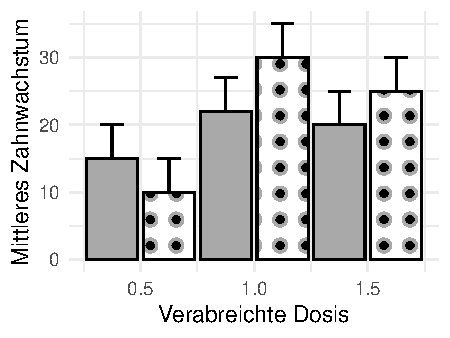
\includegraphics[width=\maxwidth]{img/mc-anova-02-a-1} 

}







\begin{enumerate}
\item [\textbf{A} \msquare] Keine Interaktion liegt vor $(p > 0.05)$.
\item [\textbf{B} \msquare] Eine positive Interaktion liegt vor $(\rho \leq -0.5)$ 
\item [\textbf{C} \msquare] Das Bestimmtheitsmaß $R^2$ ist groß.
\item [\textbf{D} \msquare] Eine negative Interaktion liegt vor $(\rho \geq 0.5)$.
\item [\textbf{E} \msquare] Es liegt eine mittlere bis starke Interaktion vor $(p \leq 0.05)$.
\end{enumerate}
\section*{Multiple Gruppenvergleiche} 

\section{Aufgabe \hfill (2 Punkte)}

%% --------------------------------------------------------------------
\ifcollection
\begin{flushright}
\tiny\vspace{-2Ex}
\textbf{\examinhaltstart}
\exammodulestatversuch $\;\bullet$
\exammodulebiostat
\vspace{-1Ex}
\end{flushright}
\fi
%% --------------------------------------------------------------------




Sie haben folgende unadjustierten p-Werte gegeben: 0.42, 0.03, 0.27, 0.02, 0.01 und 0.89. Sie adjustieren die p-Werte nach
Bonferroni. Welche Aussage ist richtig?



\begin{enumerate}
\item [\textbf{A} \msquare] Nach der Bonferroni-Adjustierung ergeben sich die adjustierten p-Werte von 1, 0.18, 1, 0.12, 0.06 und 1. Die adjustierten p-Werte werden zu einem $\alpha$-Niveau von 0.83\% verglichen.
\item [\textbf{B} \msquare] Nach der Bonferroni-Adjustierung ergeben sich die adjustierten p-Werte von 0.07, 0.005, 0.045, 0.0033, 0.0017 und 0.1483. Die adjustierten p-Werte werden zu einem $\alpha$-Niveau von 0.83\% verglichen.
\item [\textbf{C} \msquare] Nach der Bonferroni-Adjustierung ergeben sich die adjustierten p-Werte von 1, 0.18, 1, 0.12, 0.06 und 1. Die adjustierten p-Werte werden zu einem $\alpha$-Niveau von 5\% verglichen.
\item [\textbf{D} \msquare] Nach der Bonferroni-Adjustierung ergeben sich die adjustierten p-Werte von 0.07, 0.005, 0.045, 0.0033, 0.0017 und 0.1483. Die adjustierten p-Werte werden zu einem $\alpha$-Niveau von 5\% verglichen.
\item [\textbf{E} \msquare] Nach der Bonferroni-Adjustierung ergeben sich die adjustierten p-Werte von 2.52, 0.18, 1.62, 0.12, 0.06 und 5.34. Die adjustierten p-Werte werden zu einem $\alpha$-Niveau von 5\% verglichen.
\end{enumerate}

\section{Aufgabe \hfill (2 Punkte)}

%% --------------------------------------------------------------------
\ifcollection
\begin{flushright}
\tiny\vspace{-2Ex}
\textbf{\examinhaltstart}
\exammodulestatversuch $\;\bullet$
\exammodulebiostat
\vspace{-1Ex}
\end{flushright}
\fi
%% --------------------------------------------------------------------




Auf wissenschaftlichen Postern finden Sie unter Abbildungen häufig die Abbkürzung \textit{CLD}. Für welchen statistischen Fachbegriff steht die Abbkürzung und wie interpretieren Sie ein \textit{CLD}?



\begin{enumerate}
\item [\textbf{A} \msquare] Compact letter display. Gleiche Buchstaben bedeuten, dass sich die Behandlungen unterscheiden. Daher ist das CLD sehr unintuitiv. Es wäre besser, wenn gleiche Buchstaben Gleichheit anzeigen würden. Dies ist aber leider in der statistischen Testtheorie nicht möglich.
\item [\textbf{B} \msquare] Compact letter display. Gleiche Buchstaben zeigen Gleichheit in den Behandlungen. Die Interpretation ist deshalb sehr intuitiv und einfach. Darüber hinaus ist damit das CLD auch auf einer Linie mit der Testtheorie, da wir ja auch dort die Gültigkeit der Nullhypothese nachweisen. Wir suchen ja Gleichheit.
\item [\textbf{C} \msquare] Compound letter display. Gleichheit in dem Outcomes wird durch den gleichen Buchstaben oder Symbol dargestellt. Teilweise ist die Interpretation des Verbunds (eng. compound) herausfordernd, da wir ja nach dem Unterschied suchen.
\item [\textbf{D} \msquare] Contrast letter display. Unterschiede in den Behandlungen werden durch den gleichen Buchstaben oder Symbol dargestellt. Die Interpretation des CLD führt häufig in die Irre.
\item [\textbf{E} \msquare] Compact letter display. Teilweise ist die Interpretation des CLD schwierig, da wir ja nach Unterschieden suchen aber nur Gleichheit in den Buchstaben sehen. Die Gleichheit der Behandlungen wird durch gleiche Buchstaben dargestellt.
\end{enumerate}

\section{Aufgabe \hfill (2 Punkte)}

%% --------------------------------------------------------------------
\ifcollection
\begin{flushright}
\tiny\vspace{-2Ex}
\textbf{\examinhaltstart}
\exammodulestatversuch $\;\bullet$
\exammodulebiostat
\vspace{-1Ex}
\end{flushright}
\fi
%% --------------------------------------------------------------------




In Ihrer Bachelorarbeit müssen Sie einen Feldversuch auswerten. Nachdem Sie die zweifaktorielle ANOVA gerechnet haben und keine signifikante Interaktion vorliegt, wollen Sie jetzt einen Posthoc-Test rechnen. Welches R Paket nutzen Sie dafür am besten?



\begin{enumerate}
\item [\textbf{A} \msquare] Das R Paket \{lm\}. Das Paket \{lm\} erstellt selbstständig Konfidenzintervalle und entsprechende p-Werte. Da wir in dem Paket nicht adjustieren müssen, ist es bei Anwendern sehr beliebt.
\item [\textbf{B} \msquare] Das R Paket \{hmisc\} erlaubt die Durchführung eines multiplen Gruppenvergleichs aus verschiedenen Modellen heraus. Aus einem hmisc Objekt lässt sich recht einfach das CLD erstellen und so über Barplots eine schnelle Interpration der statistischen Auswertung durchführen.
\item [\textbf{C} \msquare] Das R Paket \{ggplot\}. Wir erhalten hier sofort eine Visualisierung der Daten. Anhand der Visualisierung lässt sich eine explorative Datenanalyse durchführen, die gleichwertig zu einem Posthoc-Test ist.
\item [\textbf{D} \msquare] Das R Paket \{emmeans\} erlaubt die Durchführung eines multiplen Gruppenvergleichs. Aus einem \{emmeans\} Objekt lässt sich recht einfach das CLD erstellen und so über Barplots eine schnelle Interpration der statistischen Auswertung durchführen.
\item [\textbf{E} \msquare] Das R Paket \{emmeans\} erlaubt die Durchführung eines multiplen Gruppenvergleichs. Aus einem emmeans Objekt lässt sich leider kein CLD erstellen. Dennoch ist das Paket einfach zu bedienen und wird deshalb genutzt. Die Interpretation der statistischen Auswertung wird über einen Barplot abgebildet.
\end{enumerate}

\section{Aufgabe \hfill (2 Punkte)}

%% --------------------------------------------------------------------
\ifcollection
\begin{flushright}
\tiny\vspace{-2Ex}
\textbf{\examinhaltstart}
\exammodulestatversuch $\;\bullet$
\exammodulebiostat
\vspace{-1Ex}
\end{flushright}
\fi
%% --------------------------------------------------------------------




Bei einem multiplen Vergleich oder Posthoc Test kann es zu einer Besonderheit beim statistischen Testen kommen. Wie nennt man diese Besonderheit beim statistischen Testen und wie kann man mit ihr umgehen?



\begin{enumerate}
\item [\textbf{A} \msquare] Beim multiplen Testen kann es zu einer $\alpha$-Deflation kommen. Das globale Signifikanzniveau liegt nicht mehr bei $5\%$ sondern weit darunter. Daher müssen die p-Werte entsprechend adjustiert werden. Hierfür gibt es verschiedene Verfahren, wobei das Verfahren zur Adjustierung der p-Werte nach Bonferroni das bekanneste Verfahren ist. Die p-Werte werden durch die Anzahl an Vergleichen geteilt
\item [\textbf{B} \msquare] Beim multiplen Testen kann es zu Varianzheterogenität kommen. Das globale Signifikanzniveau liegt nicht mehr bei $5\%$. Daher müssen die p-Werte entsprechend adjustiert werden. Das Verfahren nach Welch, bekannt aus dem t-Test, ist hier häufig anzuwenden.
\item [\textbf{C} \msquare] Das globale Signifikanzniveau explodiert und erreicht Werte größer als Eins. Es kommt zu einer $\alpha$-Inflation. Dagegen kann mit der Adjustierung der $\alpha$-Werte nach Bonferroni vorgegangen werden.
\item [\textbf{D} \msquare] Beim multiplen Testen kann es zu einer $\alpha$-Inflation kommen. Das globale Signifikanzniveau liegt nicht mehr bei $5\%$ sondern weit darunter. Daher müssen die p-Werte entsprechend adjustiert werden. Hierfür gibt es verschiedene Verfahren, wobei das Verfahren zur Adjustierung der p-Werte nach Welch das bekanneste Verfahren ist.
\item [\textbf{E} \msquare] Das globale Signifikanzniveau liegt nicht mehr bei $5\%$ sondern sehr viel höher. Es kommt zu einer $\alpha$-Inflation. Dagegen kann mit der Adjustierung der p-Werte nach Bonferroni vorgegangen werden.
\end{enumerate}

\section{Aufgabe \hfill (2 Punkte)}

%% --------------------------------------------------------------------
\ifcollection
\begin{flushright}
\tiny\vspace{-2Ex}
\textbf{\examinhaltstart}
\exammodulestatversuch $\;\bullet$
\exammodulebiostat
\vspace{-1Ex}
\end{flushright}
\fi
%% --------------------------------------------------------------------




Sie rechnen mehrere t-Tests für einen multiplen Vergleich nachdem eine einfaktorielle ANOVA sich als signifikant herausgestellt hat. Welche Aussage im Bezug auf den Effekt ist richtig? 



\begin{enumerate}
\item [\textbf{A} \msquare] Beim multiplen Testen kann es zu einer $\Delta$-Deflation kommen. Das globale Relevanzniveau liegt nicht mehr bei $5\%$ sondern weit darunter. Daher müssen die $\Delta$-Werte entsprechend adjustiert werden. Hierfür gibt es verschiedene Verfahren, wobei das Verfahren zur Adjustierung der $\Delta$-Werte nach Bonferroni das bekanneste Verfahren ist. Die $\Delta$-Werte werden durch die Anzahl an Vergleichen geteilt.
\item [\textbf{B} \msquare] Beim multiplen Testen kann es zu einer Effektüberschätzung ($\Delta$-Inflation) kommen. Daher müssen die Effekte angepasst werden. Dies geschieht nicht händisch sondern intern in den angewendeten Algorithmen.
\item [\textbf{C} \msquare] Wenn ein multipler Test gerechnet wird, dann muss der Effekt $\Delta$ adjustiert werden im Gegensatz zu den p-Werten.
\item [\textbf{D} \msquare] Wenn ein multipler Test gerechnet wird, dann muss der Effekt $\Delta$ nicht adjustiert werden im Gegensatz zu den p-Werten.
\item [\textbf{E} \msquare] Beim multiplen Testen werden die Effekte der paarweisen Vergleiche ignoriert. Der Nachteil des multiplen Testens ist ja auch, dass wir am Ende keine Effekte mehr vorliegen haben. Eine ANOVA liefert hier bessere Informationen.
\end{enumerate}
\section*{Lineare Regression \& Korrelation}

\section{Aufgabe \hfill (2 Punkte)}

%% --------------------------------------------------------------------
\ifcollection
\begin{flushright}
\tiny\vspace{-2Ex}
\textbf{\examinhaltstart}
\exammodulestatversuch $\;\bullet$
\exammodulebiostat
\vspace{-1Ex}
\end{flushright}
\fi
%% --------------------------------------------------------------------




Sie haben das Modell $Y \sim X$ vorliegen und wollen nun ein kausales Modell rechnen. Welche Aussage ist richtig?



\begin{enumerate}
\item [\textbf{A} \msquare] Es wird ein Trainingsdatensatz zum Modellieren des Trainingsmodells benötigt. Der Testdatensatz dient rein zur Visualisierung. Dies gilt vor allem für ein kausales Modell.
\item [\textbf{B} \msquare] Es wird ein Trainingsdatensatz zum Trainieren des Modells benötigt. Der Testdatensatz dient zur Validierung. Dies gilt insbesondere für ein kausales Modell.
\item [\textbf{C} \msquare] Wir modellieren den Zusammenhang zwischen $X$ und $Y$ wenn ein kausales Modell rerechnet wird. Dabei kann nicht der gesamte Datensatz genutzt werden. Es wird ein Trainingsdatensatz zum Trainieren des Modells benötigt.
\item [\textbf{D} \msquare] Ein kausales Modell schliesst grundsätzlich lineare Modell aus. Es muss ein Graph gefunden werden, der alle Punkte beinhaltet. Erst dann kann das $R^2$ berechnet werden.
\item [\textbf{E} \msquare] Wir modellieren den Zusammenhang zwischen $X$ und $Y$ wenn ein kausales Modell rerechnet wird. Dabei kann der gesamte Datensatz genutzt werden. Eine Aufteilung wie in einem prädiktiven Modell ist nicht notwendig.
\end{enumerate}

\section{Aufgabe \hfill (2 Punkte)}

%% --------------------------------------------------------------------
\ifcollection
\begin{flushright}
\tiny\vspace{-2Ex}
\textbf{\examinhaltstart}
\exammodulestat $\;\bullet$
\exammodulestatbbv $\;\bullet$
\exammodulestatversuch $\;\bullet$
\exammodulebiostat
\vspace{-1Ex}
\end{flushright}
\fi
%% --------------------------------------------------------------------




Nach der Modellierung einer Regression stellt sich die Frage, ob die Residuen approximativ einer Normalverteilung folgen. Sie können einen QQ-Plot für die visuelle Überprüfung der Annahme an die Residuen nutzen. Welche Aussage ist richtig?



{\centering 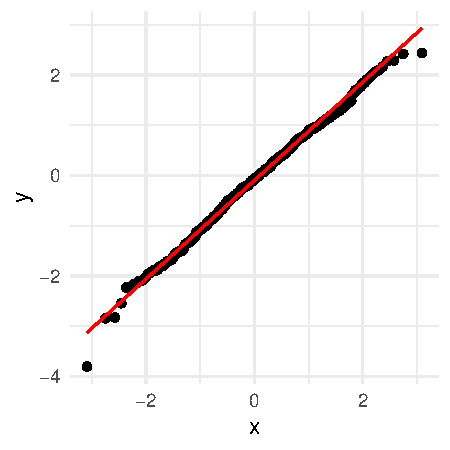
\includegraphics[width=\maxwidth]{img/mc-regression-05-a-1} 

}







\begin{enumerate}
\item [\textbf{A} \msquare] Wir betrachten die Gerade, die durch die einzelnen Punkte laufen sollte. Wenn die 95\% der Punkte von der Geraden getroffen werden, dann gehen wir von normalverteilten Residuen aus.
\item [\textbf{B} \msquare] Die Annahme der normalverteilten Residuen ist nicht erfüllt. Die Punkte liegen zum überwiegenden Teil auf der Geraden.
\item [\textbf{C} \msquare] Die Annahme der normalverteilten Residuen ist erfüllt. Die Punkte liegen zum überwiegenden Teil nicht auf der Geraden und Korrelation ist negativ.
\item [\textbf{D} \msquare] Wir betrachten die Punkte. Wenn die Punkte einigermaßen gleichmäßig verteilt liegen, dann gehen wir von normalen Residuen aus.
\item [\textbf{E} \msquare] Wir betrachten die Gerade. Wenn die Punkte einigermaßen gleichmäßig um die Gerade verteilt liegen, dann gehen wir von normalverteilten Residuen aus. Dies ist hier nicht der Fall. Wir haben keine normalverteilten Residuen vorliegen.
\end{enumerate}

\section{Aufgabe \hfill (2 Punkte)}

%% --------------------------------------------------------------------
\ifcollection
\begin{flushright}
\tiny\vspace{-2Ex}
\textbf{\examinhaltstart}
\exammodulestat $\;\bullet$
\exammodulestatbbv $\;\bullet$
\exammodulestatversuch $\;\bullet$
\exammodulebiostat
\vspace{-1Ex}
\end{flushright}
\fi
%% --------------------------------------------------------------------




In den Humanwissenschaften wird der Korrelationskoeffizienten $\rho$ sehr häufig verwendet. Daher ist es auch wichtig für andere Forschende den Korrelationskoeffizienten $\rho$ zu verstehen. Welche Aussazu zu dem Korrelationskoeffizienten $\rho$ ist richtig?




\begin{enumerate}
\item [\textbf{A} \msquare] Der Korrelationskoeffizienten $\rho$ liegt zwischen -1 und 1. Darüber hinaus ist der Korrelationskoeffizienten $\rho$ einheitslos und kann als standardisierte Steigung verstanden werden.
\item [\textbf{B} \msquare] Der Korrelationskoeffizienten $\rho$ zeigt keinen Zusammenhang zwischen zwei Variablen $x$ und $y$ bei einem Wert von 0. Einen negativen Zusammenhang Richtung -1 und somit auch einen positiven Zusammenhang Richtung 1. Je größer die Zahl allgemein, desto stärker der Effekt.
\item [\textbf{C} \msquare] Der Korrelationskoeffizienten $\rho$ liegt zwischen -1 und 1. Darüber hinaus ist der Korrelationskoeffizienten $\rho$ als standardisierte Steigung zu verstehen, wenn eine Standardisierung durchgeführt wurde. Diese Adjustierung nach Fischer muss am Anschluß der Berechnung der Korrelation durchgeführt werden.
\item [\textbf{D} \msquare] Der Korrelationskoeffizienten $\rho$ ist eine veraltete Darstellungsform von Effekten in der linearen Regression und wird wie das $\eta^2$ aus der ANOVA interpretiert. Der Korrelationskoeffizienten $\rho$ beschreibt den Anteil an erklärter Varianz durch die Regression.
\item [\textbf{E} \msquare] Der Korrelationskoeffizienten $\rho$ ist eine standardisierte, statistische Maßzahl, die zwischen 0 und 1 liegt. Dabei ist Korrelationskoeffizienten $\rho$ einheitslos. Eine Signifikanz kann nicht nachgewiesen werden.
\end{enumerate}

\section{Aufgabe \hfill (2 Punkte)}

%% --------------------------------------------------------------------
\ifcollection
\begin{flushright}
\tiny\vspace{-2Ex}
\textbf{\examinhaltstart}
\exammodulestatversuch $\;\bullet$
\exammodulebiostat
\vspace{-1Ex}
\end{flushright}
\fi
%% --------------------------------------------------------------------




Nach der Modellierung einer Regression stellt sich die Frage, ob die Residuen (\texttt{.resid}) gleichmäßig um die gefitte Gerade liegen. Sie können folgende Abbildung für die visuelle Überprüfung der Residuen nutzen. Welche Aussage ist richtig?



{\centering 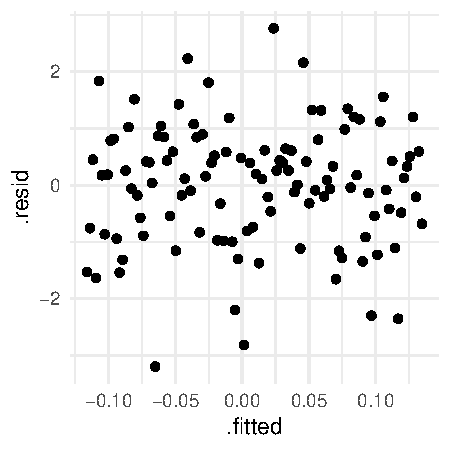
\includegraphics[width=\maxwidth]{img/mc-regression-06-a-1} 

}







\begin{enumerate}
\item [\textbf{A} \msquare] Die Annahme der normalverteilten Residuen ist erfüllt. Kein Muster ist zu erkennen und keine Outlier zu beobachten.
\item [\textbf{B} \msquare] Die Punkte müssen gleichmäßig in dem negativen Bereich liegen. Dies ist hier klar nicht der Fall. Einzelne Ausreißer können beobachtet werden. Die Analyse ist gescheitert.
\item [\textbf{C} \msquare] Wenn wir die Nulllinie betrachten so liegen die Punkte nicht gleichmäßig über und unter der Nulllinie. Unser Modell erfüllt nicht die Annahme von normalverteilten Residuen mit einem Mittelwert von 0 und einer Streuung von $s^2$.
\item [\textbf{D} \msquare] Die Annahme der normalverteilten Residuen ist erfüllt. Die Punkte liegen zum überwiegenden Teil auf der Diagonalen. Damit ist das Modell erfolgreich geschätzt worden.
\item [\textbf{E} \msquare] Die Annahme der normalverteilten Residuen ist erfüllt. Es ist ein Muster zu erkennen und wir können damit auf die Signifkanz von $x_1, ..., x_p$ schließen.
\end{enumerate}

\section{Aufgabe \hfill (2 Punkte)}

%% --------------------------------------------------------------------
\ifcollection
\begin{flushright}
\tiny\vspace{-2Ex}
\textbf{\examinhaltstart}
\exammodulebiostat
\vspace{-1Ex}
\end{flushright}
\fi
%% --------------------------------------------------------------------




In einer lineren Regression kann es vorkommen, dass der Effekt repräsentiert durch den $\beta$ Koeffizienten nicht so richtig von der Größenordnung zu dem p-Wert passen will. So liefert eine Untersuchung des Einflusses von der $PO_2$-Konzentration in [$\mu g$] im Wasser auf das Trockengewicht in [$kg$] an Erbsen folgende Effekte und p-Werte: $1e-04$ als p-Wert und einen $\beta_{PO_2}$ Koeffizienten von $7.4\times 10^{-6}$. Welche Aussage ist richtig?




\begin{enumerate}
\item [\textbf{A} \msquare] Wenn der Effekt $\beta_{PO_2}$ winzig ist, dann kann es an einer falsch gewählten Einheit liegen. Der Anstieg von einer Einheit in $X$ führt ja zu einer Änderung von $\beta_{PO_2}$ in $x$. Wir müssen daher die Einheit von $y$ entsprechend anpassen.
\item [\textbf{B} \msquare] Die Einheit der $PO_2$-Konzentration ist zu klein gewählt. Dadurch sehen wir den sehr kleinen $p$-Wert. Der $p$-Wert und die Einheit von der $PO_2$-Konzentration hängen antiproportional zusammen.
\item [\textbf{C} \msquare] Das Gewicht und die $PO_2$-Konzentration korrelieren sehr stark, deshalb wird der $\beta_{PO_2}$ Koeffizient sehr klein. Mit einer ANOVA kann für die Korrelation korrigiert werden und der Effektschätzer passt dann zum p-Wert.
\item [\textbf{D} \msquare] Die Fallzahl ist zu klein angesetzt. Je kleiner die Fallzahl ist, desto höher ist die Teststatsitik und damit auch der $p$-Wert kleiner. Wir brauchen also mehr Fallzahl um den geringen Effekt noch signifikant zu krigen.
\item [\textbf{E} \msquare] Die Einheit der $PO_2$-Konzentration ist zu klein gewählt. Die Erhöhung der $PO_2$-Konzentration um 1 Einheit führt nur zu einem sehr winzigen Anstieg von $\beta_{PO_2}$ im Gewicht der Wasserlinsen. Die Einheit [$\mu g$] muss besser gewählt werden.
\end{enumerate}

\section{Aufgabe \hfill (2 Punkte)}

%% --------------------------------------------------------------------
\ifcollection
\begin{flushright}
\tiny\vspace{-2Ex}
\textbf{\examinhaltstart}
\exammodulestatversuch $\;\bullet$
\exammodulebiostat
\vspace{-1Ex}
\end{flushright}
\fi
%% --------------------------------------------------------------------




Neben der klassischen Regression kann die Funktion \texttt{lm()} in \Rlogo auch für welche andere Art von Anwendung genutzt werden?





\begin{enumerate}
\item [\textbf{A} \msquare] Die Funktion \texttt{lm()} in \Rlogo ist der erste Schritt für einen Gruppenvergleich. Danach kann eine ANOVA oder aber ein multipler Vergleich in \{emmeans\} gerechnet werden. In der Funktion  \texttt{lm()} werden die Gruppenmittelwerte bestimmt.
\item [\textbf{B} \msquare] Neben der klassichen Verwendung der Funktion \texttt{lm()} in der linearen Regression kann auch ein Gruppenvergleich gerechnet werden. Dafür müssen aber alle Faktoren aus den Daten entfernt und numerishc umgewandelt werden. Dann kann das R Paket \{emmeans\} genutzt werden um die Korrelation zu berechnen. Eine Adjustierung ist dann nicht mehr notwendig.
\item [\textbf{C} \msquare] Ist die Einflussvariable $X$ numerisch so werden die Gruppenmittelwerte geschätzt und eine anschließende ANOVA sowie multipler Gruppenvergleich mit \{emmeans\} ist möglich.
\item [\textbf{D} \msquare] Die Funktion \texttt{lm()} berechnet die Varianzstruktur für eine ANOVA. Dannach kann dann über eine explorative Datenalayse nochmal eine Signifikanz berechnet werden. Sollte vor der Verwendung der Funktion \texttt{lm()} schon eine EDA gerechnet worden sein, so ist die Analyse wertlos.
\item [\textbf{E} \msquare] Ist die Einflussvariable $X$ ein Faktor so werden die Gruppenmittelwerte geschätzt und eine anschließende ANOVA sowie multipler Gruppenvergleich mit \{emmeans\} ist möglich. Die Funktion \texttt{lm()} kann dabei eigentlich weggelassen werden, wird aber traditionell gerechnet.
\end{enumerate}

\section{Aufgabe \hfill (2 Punkte)}

%% --------------------------------------------------------------------
\ifcollection
\begin{flushright}
\tiny\vspace{-2Ex}
\textbf{\examinhaltstart}
\exammodulebiostat
\vspace{-1Ex}
\end{flushright}
\fi
%% --------------------------------------------------------------------




Wenn Ihr gemessener Endpunkt nicht einer Normalverteilung folgt, so können Sie dennoch Ihre Daten modellieren. Hierzu nutzen Sie dann das \textit{generalisierte lineare Modell (GLM)}. Welche Aussage ist richtig?




\begin{enumerate}
\item [\textbf{A} \msquare] Das GLM erlaubt auch nicht normalverteilte Residuen in der Schätzung der Regressionsgrade.
\item [\textbf{B} \msquare] Das \textit{generalisierte lineare Modell (GLM)} erlaubt auch weitere Verteilungsfamilien für das $Y$ bzw. das Outcome in einer linearen Regression zu wählen.
\item [\textbf{C} \msquare] In \Rlogo ist mit dem \textit{generalisierten linearen Modell (GLM)} eine Modellierung implementiert, die die Poissonverteilung für Zähldaten oder die Binomialverteilung für 0/1-Daten modellieren kann. Weitere Modellierungen sind in \Rlogo auch mit zusätzlich geladenen Paketen nicht möglich.
\item [\textbf{D} \msquare] Das \textit{generalisierte lineare Modell (GLM)} erlaubt auch weitere Verteilungsgruppen für das $X$ bzw. die Einflussvariablen in einer linearen Regression zu wählen.
\item [\textbf{E} \msquare] Das GLM ist ein faktisch maschineller Lernalgorithmus, der selstständig die Verteilungsfamilie für Y wählt.
\end{enumerate}

\section{Aufgabe \hfill (2 Punkte)}

%% --------------------------------------------------------------------
\ifcollection
\begin{flushright}
\tiny\vspace{-2Ex}
\textbf{\examinhaltstart}
\exammodulebiostat
\vspace{-1Ex}
\end{flushright}
\fi
%% --------------------------------------------------------------------




In einer Studie wollen Sie den Effektschätzer Risk ratio berechnen. Sie finden in Ihrem Experiment zur Behandlung von Klaueninfektionen bei Ziegen in 4 Tieren Erkrankung der Klauen vor. 12 Tiere sind gesund. Welche Aussage ist richtig?



\begin{enumerate}
\item [\textbf{A} \msquare] Es ergibt sich ein Risk ratio von 0.25, da es sich um eine Chancenverhältnis handelt.
\item [\textbf{B} \msquare] Es ergibt sich ein Risk ratio von 0.33, da es sich um ein Anteil handelt.
\item [\textbf{C} \msquare] Das Verhältnis von Chancen Risk ratio ergibt ein Chancenverhältnis von 0.33.
\item [\textbf{D} \msquare] Das Verhältnis der Anteile Risk ratio ergibt ein Anteilsverhältnis von 0.25. Wir sind am Anteil der Kranken interessiert.
\item [\textbf{E} \msquare] Der Anteil der Gesunden wird berechnet. Da es sich um ein Anteil handelt ergibt sich ein Risk ratio von 0.25.
\end{enumerate}
    
% -----------------------------------------------------------------------
\clearpage
% -----------------------------------------------------------------------
\part{Programmieren in R}
% -----------------------------------------------------------------------

\section{Aufgabe \hfill (9 Punkte)}



 
%% --------------------------------------------------------------------
\ifcollection
\begin{flushright}
\tiny\vspace{-3Ex}
\textbf{\examinhaltstart}
\exammodulemathstat $\;\bullet$
\exammodulelanddaten $\;\bullet$
\exammodulestat 
\vspace{-4Ex}
\end{flushright}
\begin{minipage}[t]{0.5\textwidth}

\includegraphics[width = 1.3cm]{/Users/kruppajo/work/GitHub/exam/avatare/Paula.png}
\end{minipage}
\begin{minipage}[t]{0.5\textwidth}
\hfill
\href{https://www.youtube.com/playlist?list=PLe51bCp9JvEFUnFqaJG5aRmON9i1ZbOYC}{
\includegraphics[width = 2cm]{img/youtube}}
\end{minipage}
\vspace{-3ex}
\fi
%% --------------------------------------------------------------------



\ifcollection
\paragraph{Grundlegende Kenntnisse der Programierung in \Rlogo}
\fi

Paula muss ihrer Abschlussarbeit mit \Rlogo arbeiten. Deshalb sitzt sie jetzt mit Ihnen zusammen und hat einige Fragen zu den Grundlagen in \Rlogo an Sie! Na dann wollen Sie mal helfen. Immerhin will ihre Betreuerin, dass \Rlogo genutzt wird.\\[1Ex]

Paula: \textit{Wie war nochmal der Name der Funktion in dem wir in R Daten intern abspeichern? Was waren da nochmal die Vorteile?} \textbf{(1 Punkt)}\\[1ex]
Sie antworten:\\[3Ex]

Paula: \textit{Warum gibt es eigentlich das RStudio und R? Wie unterscheiden sich beide voneinander?} \textbf{(1 Punkt)}\\[1ex]
Sie antworten:\\[3Ex]

Paula: \textit{Wo nutzen wir nochmal die Tilde ($\sim$) in R. Das war irgendwie voll wichtig. Wo wird diese genutzt?} \textbf{(1 Punkt)}\\[1ex]
Sie antworten:\\[3Ex]

Paula: \textit{Der Zuweisungs-Operator wird sehr häufig genutzt. Wie sieht der aus und wie funktioniert der an einem Beispiel?} \textbf{(1 Punkt)}\\[1ex]
Sie antworten:\\[3Ex]

Paula: \textit{Was macht überhaupt dieses \texttt{c()} hier überall im \Rlogo Code?} \textbf{(1 Punkt)}\\[1ex]
Sie antworten:\\[3Ex]

Paula: \textit{Hä? Warum ändert sich nichts an meinen Daten? In R sehe ich doch die Änderungen aber irgendwie speicher R meine Änderungen meines Datensatzes ab. Was ist da los?} \textbf{(1 Punkt)}\\[1ex]
Sie antworten:\\[3Ex]

Paula: \textit{Ich verstehe den Unterschied zwischen \texttt{library()} und \texttt{Packages} nicht. Warum gibt es die?} \textbf{(1 Punkt)}\\[1ex]
Sie antworten:\\[3Ex]

Paula: \textit{Ich habe die Namen der beiden \Rlogo Pakete vergessen, die wir eigentlich immer laden. Wie heißen die noch gleich?} \textbf{(1 Punkt)}\\[1ex]
Sie antworten:\\[3Ex]

Paula: \textit{Gibt es einen Vorteil von der Nutzung von \Rlogo?} \textbf{(1 Punkt)}\\[1ex]
Sie antworten:\\[3Ex] 
\clearpage
% -----------------------------------------------------------------------

\section{Aufgabe \hfill (9 Punkte)}



 
%% --------------------------------------------------------------------
\ifcollection
\begin{flushright}
\tiny\vspace{-3Ex}
\textbf{\examinhaltstart}
\exammodulelanddaten $\;\bullet$
\exammodulestatversuch $\;\bullet$
\exammodulebiostat
\vspace{-4Ex}
\end{flushright}
\begin{minipage}[t]{0.5\textwidth}

\includegraphics[width = 1.3cm]{/Users/kruppajo/work/GitHub/exam/avatare/Jonas.png}
\end{minipage}
\begin{minipage}[t]{0.5\textwidth}
\hfill
\href{https://www.youtube.com/playlist?list=PLe51bCp9JvEFUnFqaJG5aRmON9i1ZbOYC}{
\includegraphics[width = 2cm]{img/youtube}}
\end{minipage}
\vspace{1ex}
\fi
%% --------------------------------------------------------------------



\ifcollection
\paragraph{Fortgeschrittene Kenntnisse der Programierung in \Rlogo}
\fi

Jonas muss seiner Abschlussarbeit mit \Rlogo arbeiten. Leider ist die Analyse etwas komplexer, so dass es eben in Excel dann nicht mehr geht. Deshalb also gleich alles in \Rlogo. Das ist auch der Grund warum er jetzt mit Ihnen in der Küche sitzt und einige vertiefende Fragen zu \Rlogo an Sie hat! Na dann wollen Sie mal helfen. Immerhin will sein Betreuer, dass \Rlogo genutzt wird und die Abgabe ist dann auch schon in gut einem Monat.\\[1Ex]

Jonas fragt: \textit{Wozu war nochmal die Funktion \texttt{mutate()} gut?  \textbf{(1 Punkt)}}\\[1ex]
Sie antworten:\\[6.5Ex]

Jonas fragt: \textit{Wie spezifizieren wir nochmal eine Interaktion in einem Modell mit zwei Faktoren $f_1$ und $f_2$? \textbf{(1 Punkt)}}\\[1ex]
Sie antworten:\\[6.5Ex]

Jonas fragt: \textit{Ich möchte in der Funktion \texttt{emmeans()} den Faktor $f_1$ getrennt in jedem Level des Faktors $f_2$ auswerten. Was muss ich da in de Funktion \texttt{emmeans()} angeben? \textbf{(1 Punkt)}}\\[1ex]
Sie antworten:\\[6.5Ex]

Jonas fragt: \textit{Okay, und für was brauche ich nochmal die R Pakete  \texttt{\{emmeans\}}, \texttt{\{ggplot\}} und \texttt{\{readxl\}}? \textbf{(2 Punkte)}}\\[1ex]
Sie antworten:\\[6.5Ex]

Jonas fragt: \textit{Ich möchte ein CLD erstellen. Welche Funktionen muss ich in welcher Reihenfolge nutzen? \textbf{(2 Punkte)}}\\[1ex]
Sie antworten:\\[6.5Ex]

Jonas fragt: \textit{Ich will eine ANOVA in R rechnen. Dazu brauche ich zwei Funktionen. Welche waren das noch gleich und wie war die Reihenfolge? \textbf{(1 Punkt)}}\\[1ex]
Sie antworten:\\[6.5Ex]

Jonas fragt: \textit{Es gibt ja nur ein richtiges Format für die Eingabe eines Datums. Wie lautet das Format? \textbf{(1 Punkt)}}\\[1ex]
Sie antworten:\\[6.5Ex]



 
\clearpage
% -----------------------------------------------------------------------
\part{Deskriptive Statistik \& Explorative Datenanalyse}
% -----------------------------------------------------------------------

\section{Aufgabe \hfill (9 Punkte)}

\textit{Geben Sie grundsätzlich Formeln und Rechenweg zur Lösung der Teilaufgaben mit an!} \\[1Ex]
 

 
%% --------------------------------------------------------------------
\ifcollection
\begin{flushright}
\tiny\vspace{-3Ex}
\textbf{\examinhaltstart}
\exammodulemathstat $\;\bullet$
\exammodulestat $\;\bullet$
\exammodulestatbbv $\;\bullet$
\exammodulestatversuch\\
\exammodulelanddaten $\;\bullet$
\exammodulebiostat
\vspace{-4Ex}
\end{flushright}
\begin{minipage}[t]{0.5\textwidth}

\includegraphics[width = 1.3cm]{/Users/kruppajo/work/GitHub/exam/avatare/Nilufar.png}
\end{minipage}
\begin{minipage}[t]{0.5\textwidth}
\hfill
\href{https://youtu.be/GNoORO7GfAE}{
\includegraphics[width = 2cm]{img/youtube}}
\end{minipage}
\vspace{-3ex}
\fi
%% --------------------------------------------------------------------



\ifcollection
\paragraph{Zerforschen des Barplots}
\fi

Nilufar steht vor einem ersten Problem, denn wenn es nach ihrer Betreuerin geht, soll sie in einem einem Gewächshausexperiment Erdbeeren auswertet. Soweit eigentlich alles passend. Besser wäre was anderes gewesen. Am Ende dann doch besser Hip Hop. Wunderbar. Eine echte Ablenkung für Nilufar. Das heißt erstmal überlegen für Nilufar. Aus den Boxen wummert Deichkind und ihr Mund ist verklebt von Takis Blue Heat. 'Herrlich', denkt Nilufar. Die Behandlung werden verschiedene Genotypen ($AA$, $AB$ und $BB$) sein. In ihrer Exceldatei wird sie den Endpunkt ($Y$) \textit{Frischegewicht} als \textit{freshmatter} aufnehmen. Vorab soll Nilufar aber eimal die folgenden Barplots ihrer Betreuerin nachbauen, damit sie den \Rlogo Code schonmal für später vorliegen hat. Damit geht das Problem schon los. Eine echte Herausforderung für sie war schon immer die Erwartung gewesen. Ein leidiges Lied.



{\centering 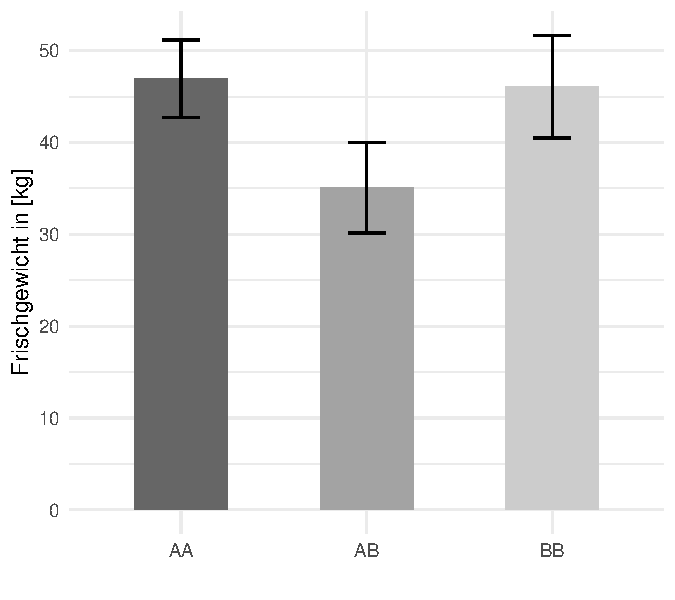
\includegraphics[width=\maxwidth]{img/barplot-02-1} 

}




Leider kennt sich Nilufar mit der Erstellung von Barplots in \Rlogo nicht aus. Deshalb braucht sie bei der Visualisierung Ihre Hilfe!

\begin{enumerate}
\item Formulieren Sie die wissenschaftliche Fragestellung! \textbf{(1 Punkt)}
\item Erstellen Sie eine Tabelle mit den statistischen Maßzahlen der drei Barplots! \textit{Beachten Sie die korrekte Darstellungsform der statistischen Maßzahlen!} \textbf{(4 Punkte)}
\item Erstellen Sie einen beispielhaften Datensatz im \Rlogo üblichen Format, aus dem die drei Barplots \textit{möglicherweise} erstellt wurden! \textbf{(2 Punkte)}
\item Kann Nilufar einen Unterschied zwischen den Behandlungen erwarten? Begründen Sie Ihre Antwort! \textbf{(2 Punkte)}
\end{enumerate} 
\clearpage
% -----------------------------------------------------------------------

\section{Aufgabe \hfill (8 Punkte)}

\textit{Geben Sie grundsätzlich Formeln und Rechenweg zur Lösung der Teilaufgaben mit an!} \\[1Ex]
 

 
%% --------------------------------------------------------------------
\ifcollection
\begin{flushright}
\tiny\vspace{-3Ex}
\textbf{\examinhaltstart}
\exammodulemathstat $\;\bullet$
\exammodulestat $\;\bullet$
\exammodulelanddaten $\;\bullet$
\exammodulestatbbv 
\vspace{-4Ex}
\end{flushright}
\begin{minipage}[t]{0.5\textwidth}

\includegraphics[width = 1.3cm]{/Users/kruppajo/work/GitHub/exam/avatare/Tina.png}
\end{minipage}
\begin{minipage}[t]{0.5\textwidth}
\hfill
\href{https://youtu.be/UabXe73G-7w}{
\includegraphics[width = 2cm]{img/youtube}}
\end{minipage}
\vspace{-3ex}
\fi
%% --------------------------------------------------------------------



\ifcollection
\paragraph{Visualisierung des Barplots}
\fi

Tina steht vor einem ersten Problem, denn wenn es nach ihrer Betreuerin geht, soll sie in einem einem Feldexperiment Maiss auswertet. Soweit eigentlich alles passend. Besser wäre was anderes gewesen. Tina liebt Astronomie. Darin kann sie sich wirklich verlieren und immer wieder neu begeistern. Die Behandlung waren verschiedene Lichtstufen ($none$, $200lm$ und $600lm$). In ihrer Exceldatei hat sie den Endpunkt ($Y$) \textit{Proteingehalt} als \textit{protein} aufgenommen. Nun soll Tina die Daten eimal als Barplots in einer Präsentation visualisieren, damit ihrer Betreuerin wieder klar wird, was sie eigentlich nochmal gemacht hat und was für ein Ergbnis in einem statistischen Test zu erwarten wäre. Wäre da nicht noch etwas. Tina und die Wut, eine unendliche Geschichte mit kniffeligen Wendungen. Aber egal. Einfach mal raus um zu Boxen. Ohne Ziel und Uhr. Das ist was für Tina.

\begin{table}[!h]
\centering
\begin{tabular}{cc}
\toprule
treatment & protein\\
\midrule
200lm & 49.6\\
none & 7.4\\
200lm & 49.8\\
200lm & 35.0\\
600lm & 39.1\\
\addlinespace
none & 29.9\\
none & 16.6\\
600lm & 27.7\\
600lm & 37.2\\
none & 20.4\\
\addlinespace
600lm & 36.2\\
none & 18.8\\
600lm & 52.5\\
\bottomrule
\end{tabular}
\end{table}



Leider kennt sich Tina mit der Erstellung von Barplots nicht aus. Deshalb braucht sie bei der Visualisierung Ihre Hilfe!

\begin{enumerate}
\item Formulieren Sie die wissenschaftliche Fragestellung! \textbf{(1 Punkt)}
\item Zeichnen Sie in \underline{einer} Abbildung die Barplots für die Behandlung von Maiss! Beschriften Sie die Achsen entsprechend! \textbf{(4 Punkte)}
\item Beschriften Sie \underline{einen} Barplot mit den gängigen statistischen Maßzahlen! \textbf{(2 Punkte)}
\item Wenn Tina \underline{einen} Effekt zwischen den Behandlungen von Maiss erwarten würde, wie sehen dann die Barplots aus? \textit{Antworten Sie mit einer Skizze der Barplots!}
  \textbf{(1 Punkt)}
\end{enumerate} 
\clearpage
% -----------------------------------------------------------------------

\section{Aufgabe \hfill (9 Punkte)}

\textit{Geben Sie grundsätzlich Formeln und Rechenweg zur Lösung der Teilaufgaben mit an!} \\[1Ex]
 

 
%% --------------------------------------------------------------------
\ifcollection
\begin{flushright}
\tiny\vspace{-3Ex}
\textbf{\examinhaltstart}
\exammodulemathstat $\;\bullet$
\exammodulestat $\;\bullet$
\exammodulestatbbv $\;\bullet$
\exammodulestatversuch\\
\exammodulelanddaten $\;\bullet$
\exammodulebiostat
\vspace{-4Ex}
\end{flushright}
\begin{minipage}[t]{0.5\textwidth}

\includegraphics[width = 1.3cm]{/Users/kruppajo/work/GitHub/exam/avatare/Mark.png}
\end{minipage}
\begin{minipage}[t]{0.5\textwidth}
\hfill
\href{https://youtu.be/MyrNZ46i3uY}{
\includegraphics[width = 2cm]{img/youtube}}
\end{minipage}
\vspace{-3ex}
\fi
%% --------------------------------------------------------------------



\ifcollection
\paragraph{Zerforschen des Boxplots}
\fi

Wenn die Unsicherheit nicht wäre, ja dann wäre wohl vieles möglich für Mark! Aber so.. Deshalb gilt anschauen, was andere vor einem gemacht haben. Für Mark ist es eine Möglichkeit schneller ans Ziel zu gelangen. Mark soll in seiner Hausarbeit Erdbeeren untersuchen. Die Behandlung in seiner Hausarbeit werden verschiedene Lichtstufen ($none$, $200lm$ und $600lm$) sein. Erheben wird Mark als Messwert ($Y$) \textit{Proteingehalt} benannt als \textit{protein} in seiner Exceldatei. Von seinem Betreuer erhält er nun folgende Abbildung von Boxplots, die er erstmal zur Übung nachbauen soll, bevor er mit dem eigentlichen Versuch beginnt. Aber nur in passender Atmospäre! Hm, lecker Marzipankugeln und dazu dann im Hintergrund Columbo laufen lassen.



{\centering 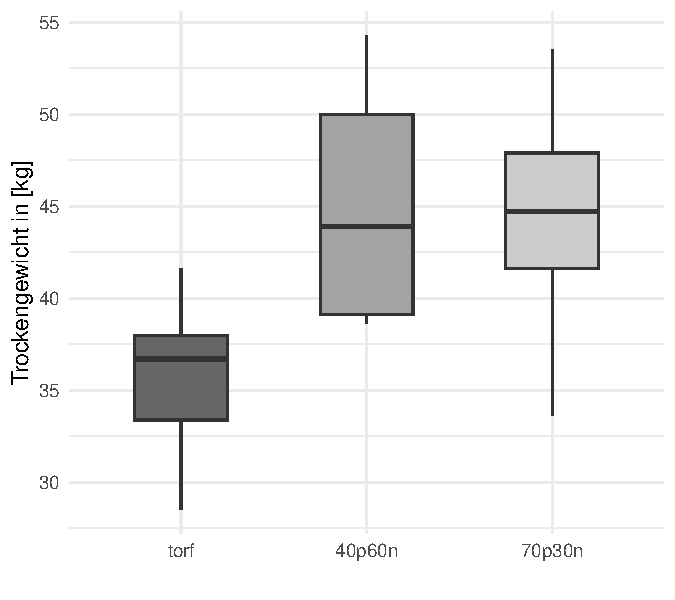
\includegraphics[width=\maxwidth]{img/boxplot-02-zer-1} 

}




Leider kennt sich Mark mit der Erstellung von Boxplots in \Rlogo nicht aus. Deshalb braucht er bei der Visualisierung Ihre Hilfe!

\begin{enumerate}
\item Formulieren Sie die wissenschaftliche Fragestellung! \textbf{(1 Punkt)}
\item Erstellen Sie eine Tabelle mit den statistischen Maßzahlen aus der obigen Abbildung der drei Boxplots! \textit{Beachten Sie die korrekte Darstellungsform der statistischen Maßzahlen!} \textbf{(2 Punkte)}
\item Beschriften Sie \textit{einen} der Boxplots mit den gängigen statistischen Maßzahlen! \textbf{(2 Punkte)}
\item Erstellen Sie einen beispielhaften Datensatz, aus dem die drei Boxplots \textit{möglicherweise} erstellt wurden, im \Rlogo üblichen Format! \textbf{(2 Punkte)}
\item Kann Mark einen Unterschied zwischen den Behandlungen erwarten? Begründen Sie Ihre Antwort! \textbf{(2 Punkte)}
\end{enumerate} 
\clearpage
% -----------------------------------------------------------------------

\section{Aufgabe \hfill (9 Punkte)}

\textit{Geben Sie grundsätzlich Formeln und Rechenweg zur Lösung der Teilaufgaben mit an!} \\[1Ex]
 

 
%% --------------------------------------------------------------------
\ifcollection
\begin{flushright}
\tiny\vspace{-3Ex}
\textbf{\examinhaltstart}
\exammodulemathstat $\;\bullet$
\exammodulestat $\;\bullet$
\exammodulelanddaten $\;\bullet$
\exammodulestatbbv 
\vspace{-4Ex}
\end{flushright}
\begin{minipage}[t]{0.5\textwidth}

\includegraphics[width = 1.3cm]{/Users/kruppajo/work/GitHub/exam/avatare/Alex.png}
\end{minipage}
\begin{minipage}[t]{0.5\textwidth}
\hfill
\href{https://youtu.be/ZbrvpCuZl_k}{
\includegraphics[width = 2cm]{img/youtube}}
\end{minipage}
\vspace{-3ex}
\fi
%% --------------------------------------------------------------------



\ifcollection
\paragraph{Visualisierung des Boxplots}
\fi

Boxplots sind bedeutend in der Darstellung von wissenschaftlichen Ergebnissen. Leider hat sich Alex nicht gemerkt, welche statistischen Maßzahlen für einen Boxplot erhoben werden müssen. Besser wäre was anderes gewesen. Alex liebt Starcraft. Darin kann er sich wirklich verlieren und immer wieder neu begeistern. Das ist in soweit doof, da nach seinem Betreuer nun Boxplots aus seinen Daten gebaut werden sollen, bevor es mit dem statistischen Testen weitergeht. Anhand von Boxplots lässt sich eine Aussage über die Normalverteilung von $Y$ treffen. Die Behandlung für Erdbeeren waren verschiedene Bewässerungstypen ($low$ und $high$). Erfasst wurde von Alex als Messwert ($Y$) \textit{Proteingehalt}. Alex hat dann \textit{protein} in seiner Exceldatei eintragen. Aber nur in passender Atmospäre! Auf seinem Second Screen läuft Alien und Alex schaufelt Gummibärchen. Nicht effizient, aber gut.

\begin{table}[!h]
\centering
\begin{tabular}{cc}
\toprule
treatment & drymatter\\
\midrule
high & 34.5\\
high & 18.4\\
low & 33.9\\
high & 23.8\\
low & 35.5\\
\addlinespace
low & 33.5\\
high & 27.9\\
high & 24.8\\
low & 38.1\\
high & 33.1\\
\addlinespace
high & 39.6\\
low & 31.6\\
low & 38.2\\
high & 30.3\\
low & 37.1\\
\addlinespace
low & 29.8\\
low & 29.2\\
high & 34.3\\
low & 28.0\\
high & 33.9\\
\bottomrule
\end{tabular}
\end{table}



Leider kennt sich Alex mit der Erstellung von Boxplots nicht aus. Deshalb braucht er bei der Visualisierung Ihre Hilfe!

\begin{enumerate}
\item Formulieren Sie die wissenschaftliche Fragestellung! \textbf{(1 Punkt)}
\item Zeichnen Sie in \textit{einer} Abbildung die beiden Boxplots für die zwei Behandlungen von Erdbeeren! Beschriften Sie die Achsen entsprechend! \textbf{(4 Punkte)} 
\item Wie ist Ihr Vorgehen, wenn Sie eine \textit{gerade} Anzahl an
  Beobachtungen pro Gruppe haben? \textbf{(1 Punkt)}
\item Beschriften Sie \textit{einen} der beiden Boxplots mit den gängigen
  statistischen Maßzahlen! \textbf{(2 Punkte)}
\item Wenn Sie \underline{keinen} Effekt zwischen den Behandlungen von Erdbeeren erwarten würden, wie sehen dann die beiden Boxplots aus? \textit{Antworten Sie mit einer Skizze der Boxplots!} \textbf{(1 Punkt)}
\end{enumerate} 
\clearpage
% -----------------------------------------------------------------------

\section{Aufgabe \hfill (10 Punkte)}

\textit{Geben Sie grundsätzlich Formeln und Rechenweg zur Lösung der Teilaufgaben mit an!} \\[1Ex]
 

 
%% --------------------------------------------------------------------
\ifcollection
\begin{flushright}
\tiny\vspace{-3Ex}
\textbf{\examinhaltstart}
\exammodulemathstat $\;\bullet$
\exammodulestat $\;\bullet$
\exammodulestatbbv $\;\bullet$
\exammodulestatversuch $\;\bullet$
\exammodulebiostat
\vspace{-4Ex}
\end{flushright}
\begin{minipage}[t]{0.5\textwidth}

\includegraphics[width = 1.3cm]{/Users/kruppajo/work/GitHub/exam/avatare/Alex.png}
\end{minipage}
\begin{minipage}[t]{0.5\textwidth}
\hfill
\href{https://youtu.be/md9I_UV5_lE}{
\includegraphics[width = 2cm]{img/youtube}}
\end{minipage}
\vspace{-3ex}
\fi
%% --------------------------------------------------------------------




\ifcollection
\paragraph{Visualisierung des Scatterplots}
\fi

Alex liest laut: 'Wenn zwei kontinuierliche Variablen vorliegen, können diese in einer exploartiven Datenanalyse...'. Alex stoppt. Alex schmeißt noch eine Handvoll Gummibärchen in seinen Rachen. Im Hintergrund klirrt leise der Spiegel zum Sound von Abba. Was waren noch gleich kontinuierliche Variablen? In seiner Abschlussarbeit hatte er ein Stallexperiment im Oldenburger Land durchgeführt. Dabei ging es um den Zusammenhang zwischen Gewichtszuwachs in der 1LW und durchschnittlichen Bewegungsscore [Movement/h] im groben Kontext von Hühnern. Nun stellt sich die Frage für ihn, ob es überhaupt einen Zusammenhang zwischen den gemessenen Variablen gibt. Dafür war eine explorative Datenanalyse gut! Wenn die Gefälligkeit nicht wäre, ja dann wäre wohl vieles möglich für Alex! Aber so.. Dann was anderes. Irgendwie komisch, wenn er Alien anmacht, dann ist die Katze eigentlich sofort vor dem Bildschirm und starrt hinein.

\begin{table}[!h]
\centering
\begin{tabular}{cc}
\toprule
Durchschnittlichen Bewegungsscore [Movement/h] & Gewichtszuwachs in der 1LW\\
\midrule
25.2 & 22.0\\
25.1 & 19.8\\
23.9 & 21.3\\
27.5 & 22.9\\
25.6 & 19.6\\
\addlinespace
28.3 & 21.4\\
25.7 & 18.9\\
23.7 & 19.1\\
24.7 & 21.1\\
26.1 & 21.0\\
\addlinespace
22.7 & 21.1\\
\bottomrule
\end{tabular}
\end{table}



Leider kennt sich Alex mit der Erstellung einer explorativen Datenanalyse für kontinuierliche Daten überhaupt nicht aus. Deshalb braucht er bei der Erstellung Ihre Hilfe!

\begin{enumerate}
\item Erstellen Sie eine Visualisierung für die Datentabelle. Beschriften Sie
  die Achsen entsprechend! \textbf{(4 Punkte)}
\item Schätzen Sie eine Gerade durch die Punkte! \textbf{(1 Punkt)}
\item Beschriften Sie die Gerade mit den gängigen statistischen Maßzahlen! Geben Sie die numerischen Zahlenwerte mit an! \textbf{(3 Punkte)}
\item Wenn \textit{kein} Effekt von $x$ auf $y$ vorhanden wäre, wie würde die Gerade verlaufen und welche Werte würden die statistischen Maßzahlen annehmen? \textbf{(2 Punkt)}
\end{enumerate} 
\clearpage
% -----------------------------------------------------------------------

\section{Aufgabe \hfill (10 Punkte)}

\textit{Geben Sie grundsätzlich Formeln und Rechenweg zur Lösung der Teilaufgaben mit an!} \\[1Ex]
 

 
%% --------------------------------------------------------------------
\ifcollection
\begin{flushright}
\tiny\vspace{-3Ex}
\textbf{\examinhaltstart}
\exammodulestat $\;\bullet$
\exammodulestatbbv 
\vspace{-4Ex}
\end{flushright}
\begin{minipage}[t]{0.5\textwidth}

\includegraphics[width = 1.3cm]{/Users/kruppajo/work/GitHub/exam/avatare/Alex.png}
\end{minipage}
\begin{minipage}[t]{0.5\textwidth}
\hfill
\href{https://youtu.be/L4nSytEHcaE}{
\includegraphics[width = 2cm]{img/youtube}}
\end{minipage}
\vspace{-3ex}
\fi
%% --------------------------------------------------------------------



\ifcollection
\paragraph{Visualisierung des Mosaicplots}
\fi

Das Verrückte ist, dass die Katze Alien wirklich liebt. Das ist Alex sehr recht, denn er braucht Entspannung. Aber Ablenkung hilft nur begrenzt. 'Uff!', denkt sich Alex. Jetzt hat er doch tatsächlich zwei kategoriale Variablen in seiner Abschlussarbeit gemessen. Zum einen die Behandlung Pestizideinsatz [ja/nein] und zum anderen die Messung Trockengewicht über Zielwert [ja/nein] im Kontext von Erbsen. Hierfür hat er ein Freilandversuch in der Uckermark durchgeführt. Jetzt möchte Alex die Daten einmal in einer explorativen Datenanalyse darstellen. Danach kann er dann über den passenden statistischen Test nachdenken. Dabei unterstützt seine Betreuerin diesen Ansatz bevor es in der Datenanalyse weiter geht. So schön wie so gut. Wenn die Gefälligkeit nicht wäre, ja dann wäre wohl vieles möglich für Alex! Aber so..



\vspace{1Ex}

\begin{center}
\begin{minipage}[t]{0.45\textwidth}
%\small
\begin{center}

\begin{tabular}{p{2.5cm}p{2.5cm}p{2.5cm}p{2.5cm}}
\toprule
Pestizideinsatz & Trockengewicht über Zielwert\\
\midrule
nein & ja\\
ja & nein\\
nein & ja\\
nein & ja\\
ja & ja\\
\addlinespace
nein & ja\\
nein & nein\\
ja & ja\\
ja & nein\\
ja & nein\\
\addlinespace
nein & ja\\
ja & nein\\
ja & ja\\
ja & ja\\
ja & ja\\
\addlinespace
nein & ja\\
\bottomrule
\end{tabular}


\end{center}
\end{minipage}
\begin{minipage}[t]{0.45\textwidth}
%\small
\begin{center}

\begin{tabular}{p{2.5cm}p{2.5cm}p{2.5cm}p{2.5cm}}
\toprule
Pestizideinsatz & Trockengewicht über Zielwert\\
\midrule
nein & ja\\
ja & ja\\
nein & nein\\
nein & ja\\
ja & nein\\
\addlinespace
nein & nein\\
nein & nein\\
ja & ja\\
ja & ja\\
nein & ja\\
\addlinespace
ja & ja\\
nein & ja\\
ja & ja\\
ja & ja\\
nein & ja\\
\addlinespace
nein & nein\\
\bottomrule
\end{tabular}


\end{center}
\end{minipage}
\end{center}

\vspace{2Ex}

Leider kennt sich Alex mit der Erstellung einer explorativen Datenanalyse für kategoriale Daten überhaupt nicht aus. Deshalb braucht er bei der Erstellung Ihre Hilfe!

\begin{enumerate}
\item Stellen Sie den Zusammenhang zwischen den beiden kategorialen Variablen in einer zusammenfassenden Tabelle dar! \textbf{(3 Punkte)}
\item Berechnen Sie die Verhältnisse in der zusammenfassenden Tabelle! Welche Annahme haben Sie getroffen? \textbf{(2 Punkte)}
\item Visualisieren Sie den Zusammenhang zwischen den beiden kategorialen Variablen! \textbf{(3 Punkte)}
\item Wenn \textit{kein} Effekt von der Behandlung vorliegen würde, wie würde die Tabelle und die Visualisierung aussehen? \textbf{(2 Punkt)}
\end{enumerate} 
\clearpage
% -----------------------------------------------------------------------

\section{Aufgabe \hfill (8 Punkte)}

\textit{Geben Sie grundsätzlich Formeln und Rechenweg zur Lösung der Teilaufgaben mit an!} \\[1Ex]
 

 
%% --------------------------------------------------------------------
\ifcollection
\begin{flushright}
\tiny\vspace{-3Ex}
\textbf{\examinhaltstart}
\exammodulestatversuch $\;\bullet$
\exammodulebiostat
\vspace{-4Ex}
\end{flushright}
\begin{minipage}[t]{0.5\textwidth}

\includegraphics[width = 1.3cm]{/Users/kruppajo/work/GitHub/exam/avatare/Tina.png}
\end{minipage}
\begin{minipage}[t]{0.5\textwidth}
\hfill
\href{https://youtu.be/n0Wr7VaN3Ao}{
\includegraphics[width = 2cm]{img/youtube}}
\end{minipage}
\vspace{-3ex}
\fi
%% --------------------------------------------------------------------



\ifcollection
\paragraph{Visualisierung des Histogramm für kategoriale Daten}
\fi

In einem Gespräch mit ihrer Betreuerin wird Tina gebeten seine Daten aus einem Leistungssteigerungsversuch mit Schweinen in einem Histogramm darzustellen. 'Hm...', Katjes und Tocotronic. Das ist und bleibt die beste Kombination zum Nachdenken für Tina. In ihrem Experiment hat er die dunklen Pigmentstörungen erst fotographiert und dann ausgezählt. Laut ihrer Betreuerin soll das Histogramm helfen, die Verteilung der die dunklen Pigmentstörungen zu bestimmen. Es wäre einfacher, wenn da nicht noch was wäre. Tina und die Wut, eine unendliche Geschichte mit kniffeligen Wendungen. Tina streichelt liebevoll die Spinne. Der Kopf ist in ihrem Schloß vergraben um den Klang von Tocotronic zu dämpfen.

\begin{center}
Die dunklen Pigmentstörungen: 6, 1, 5, 1, 3, 2, 3, 3, 1, 3, 4, 3, 4, 4, 5, 6, 5, 5, 3, 5, 5, 3, 5, 1, 5, 5, 5, 6, 8, 9, 6, 6, 5, 7, 5, 2
\end{center}

Leider kennt sich Tina mit der Erstellung von Histogrammen überhaupt nicht aus. Deshalb braucht sie bei der Erstellung Ihre Hilfe!

\begin{enumerate}
\item Zeichen Sie ein Histogramm um die Verteilung der Daten zu visualisieren! (\textbf{3 Punkte})
\item Beschriften Sie die Achsen der Abbildung! (\textbf{2 Punkte})
\item Ergänzen Sie die absoluten und relativen Häufigkeiten in der
  Abbildung! \textbf{(1 Punkt)}
\item Berechnen Sie aus den Daten die \textit{Wahrscheinlichkeit}
  mehr als die Anzahl 6 zu beobachten! \textbf{(1
    Punkt)}
\item Berechnen Sie aus den Daten die \textit{Chance} mehr
  als die Anzahl 6 zu beobachten! \textbf{(1 Punkt)}
\end{enumerate}

 
\clearpage
% -----------------------------------------------------------------------

\section{Aufgabe \hfill (8 Punkte)}

\textit{Geben Sie grundsätzlich Formeln und Rechenweg zur Lösung der Teilaufgaben mit an!} \\[1Ex]
 

 
%% --------------------------------------------------------------------
\ifcollection
\begin{flushright}
\tiny\vspace{-3Ex}
\textbf{\examinhaltstart}
\exammodulestatversuch $\;\bullet$
\exammodulebiostat
\vspace{-4Ex}
\end{flushright}
\begin{minipage}[t]{0.5\textwidth}

\includegraphics[width = 1.3cm]{/Users/kruppajo/work/GitHub/exam/avatare/Nilufar.png}
\end{minipage}
\begin{minipage}[t]{0.5\textwidth}
\hfill
\href{https://youtu.be/Q-kyhucwIXs}{
\includegraphics[width = 2cm]{img/youtube}}
\end{minipage}
\vspace{-3ex}
\fi
%% --------------------------------------------------------------------



\ifcollection
\paragraph{Visualisierung des Histogramm für kontinuierliche Daten}
\fi

Nilufar schmeißt noch eine Handvoll Takis Blue Heat in ihren Rachen. Im Hintergrund klirrt leise der Spiegel zum Sound von Deichkind. Nilufar betrachtet die folgenden Daten nach einem Stallexperiment mit Schweinen. In dem Experiment wurden die mittlere Anzahl an weißen Blutkörperchen gezählt. Nach der Meinung ihrer Betreuerin muss als erstes geschaut werden, wie diese verteilt sind. Also welcher statistischen Verteilung die mittlere Anzahl an weißen Blutkörperchen folgen. Dazu soll Nilufar ein Histogramm verwenden. Dann hätte man auch einen guten Überblick über den Messwert ($Y$). Es wäre einfacher, wenn da nicht noch was wäre. Eine echte Herausforderung für sie war schon immer die Erwartung gewesen. Ein leidiges Lied. Nilufar streichelt liebevoll das Huhn. Der Kopf ist in ihrem Schloß vergraben um den Klang von Deichkind zu dämpfen.

\begin{center}
Die mittlere Anzahl an weißen Blutkörperchen: 11.4, 7.4, 8.3, 9.5, 9.8, 8.5, 9.8, 7.3, 9.7, 11.2, 10.6, 10.4, 12.9, 13.1, 12.2, 10.1, 9.8, 10.4, 8.8, 10.3, 9.3, 10.3, 12.6, 10.1, 9.3, 12.7, 10.4, 11.1
\end{center}

Leider kennt sich Nilufar mit der Erstellung von Histogrammen überhaupt nicht aus. Deshalb braucht sie bei der Erstellung Ihre Hilfe!

\begin{enumerate}
\item Zeichen Sie ein Histogramm um die Verteilung der Daten zu visualisieren! (\textbf{3 Punkte})
 \item Erläutern Sie Ihr Vorgehen um ein Histogramm für kontinuierliche Daten zu zeichnen!  (\textbf{2 Punkte})
\item Beschriften Sie die Achsen der Abbildung! (\textbf{2 Punkte})
\item Ergänzen Sie die relativen Häufigkeiten in der Abbildung! \textbf{(1 Punkt)}  
\end{enumerate}

 
\clearpage
% -----------------------------------------------------------------------

\section{Aufgabe \hfill (10 Punkte)}

\textit{Geben Sie grundsätzlich Formeln und Rechenweg zur Lösung der Teilaufgaben mit an!} \\[1Ex]
 

 
%% --------------------------------------------------------------------
\ifcollection
\begin{flushright}
\tiny\vspace{-3Ex}
\textbf{\examinhaltstart}
\exammodulestatversuch $\;\bullet$
\exammodulebiostat
\vspace{-4Ex}
\end{flushright}
\begin{minipage}[t]{0.5\textwidth}

\includegraphics[width = 1.3cm]{/Users/kruppajo/work/GitHub/exam/avatare/Alex.png}\hspace{-4mm}
\includegraphics[width = 1.3cm]{/Users/kruppajo/work/GitHub/exam/avatare/Paula.png}
\end{minipage}
\begin{minipage}[t]{0.5\textwidth}
\hfill
\href{https://youtu.be/A4E9zBOltuU}{
\includegraphics[width = 2cm]{img/youtube}}
\end{minipage}
\fi
%% --------------------------------------------------------------------



\ifcollection
\paragraph{Visualisierung von Verteilungen}
\fi

'Ich glaube, dass es sich hier wieder um so ein kryptisches Lernziel handelt, was nicht so gleich klar ist.', meint Alex und streichelt sanft die Katze. Das Tier versucht dem strammen Griff zu entkommen, gibt aber auf. Paula sieht sich sehr genau die drei liegenden Boxplots an. 'Du weißt doch wie es heißt, \textit{Frei ist, wer missfallen kann.}\footnote{Oschmann, A. (2024) Mädchen stärken: Stärken fördern, Selbstwert erhöhen und liebevoll durch Krisen begleiten. Goldegg Verlag}', merkt Alex nickend an. Das Ziel ist es zu verstehen, wie eine Verteilung anhand eines Boxplots bewertet werden kann. Alex und die Gefälligkeit machen die Sache nicht einfacher.



{\centering 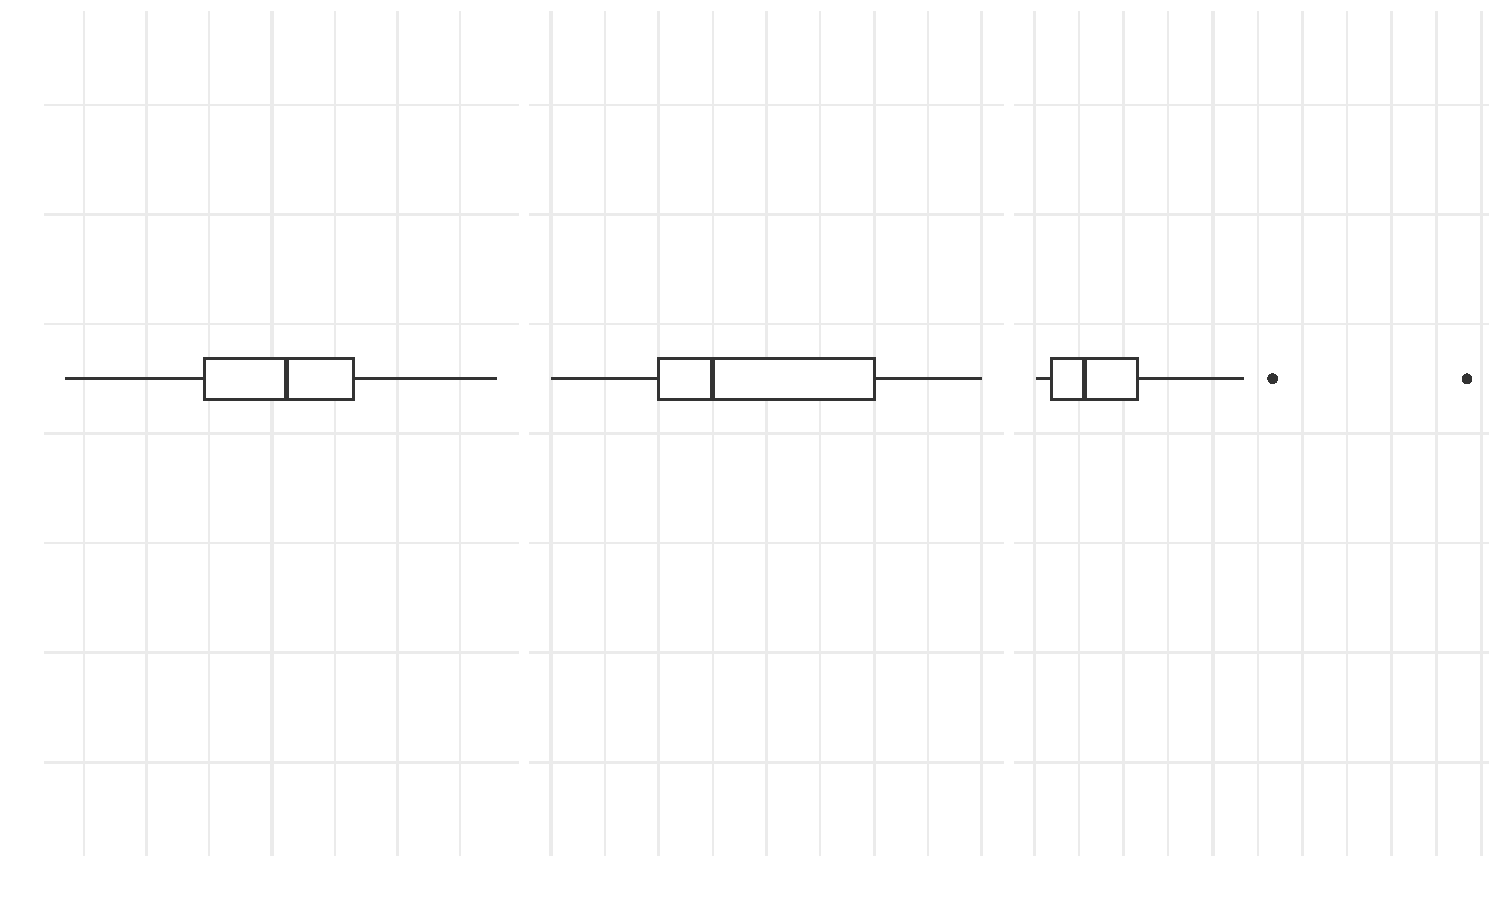
\includegraphics[width=\maxwidth]{img/desc-stat-11-1} 

}




Jetzt brauchen Alex und Paula Ihre Hilfe bei der Abschätzung einer Verteilung anhand von Boxplots um ihre Arbeit dann in diesem Semester noch abschließen zu können.

\begin{enumerate}
\item Zeichnen Sie über die Boxplots die entsprechende zugehörige Verteilung! \textbf{(3 Punkte)} 
\item Zeichnen Sie unter die Boxplots die entsprechende zugehörige Beobachtungen als Striche! \textbf{(3 Punkte)}
\item Wie viel Prozent der Beobachtungen fallen in das IQR? Ergänzen Sie die Abbildung entsprechend um den Bereich! \textbf{(2 Punkte)}
\item Wie viel Prozent der Beobachtungen fallen in $\bar{y} \pm 1s$ und $\bar{y} \pm 2s$  unter der Annahme einer Normalverteilung? \textbf{(2 Punkte)}
\end{enumerate} 
\clearpage
% -----------------------------------------------------------------------
\part{Statistisches Testen \& statistische Testtheorie}
% -----------------------------------------------------------------------  

\section{Aufgabe \hfill (9 Punkte)}


 
%% --------------------------------------------------------------------
\ifcollection
\begin{flushright}
\tiny
\textbf{\examinhaltstart}
\exammodulestat $\;\bullet$
\exammodulestatbbv $\;\bullet$
\exammodulestatversuch $\;\bullet$
\exammodulebiostat
\vspace{-4Ex}
\end{flushright}
\begin{minipage}[t]{0.5\textwidth}
\includegraphics[width = 1.3cm]{/Users/kruppajo/work/GitHub/exam/avatare/Alex.png}\hspace{-4mm}\includegraphics[width = 1.3cm]{/Users/kruppajo/work/GitHub/exam/avatare/Mark.png}
\end{minipage}
\begin{minipage}[t]{0.5\textwidth}
\hfill
\href{https://youtu.be/KxDklbFEEHw}{\includegraphics[width = 2cm]{img/youtube}}
\end{minipage}
\fi
%% --------------------------------------------------------------------



\ifcollection
\paragraph{Grundgesamtheit und experimentelle Stichprobe}
\fi

An einem schwülem Sommernachmittag sitzen Alex und Mark in einem Eiskaffee und wollen sich auf die Klausur vorbereiten. In fast allen Fragen geht es ja um die Interpretation eines statistischen Tests. Daher wollen die beiden jetzt nochmal nacharbeiten, was die Grundlagen der Stichprobe (eng. \textit{sample}) und der Grundgesamtheit (eng. \textit{population} oder \textit{ground truth}) sind. Alex hat sich Gummibärchen Eisbecher bestellt und Mark bleibt lieber bei einem Marzipankugeln Eis. 'Irre, was die Lebensmittelindustrie alles auf die Beine kriegt', merk Mark an und Alex schüttelt anerkennend den Kopf.

\vspace{1ex}

Leider kennen sich Alex und Mark mit der Grundgesamtheit und der Stichprobe überhaupt nicht aus. Daher sind Sie gefragt!

\begin{enumerate}
\item Erklären Sie den Zusammenhang zwischen Stichprobe und Grundgesamtheit an einem Schaubild! Beschriften Sie das Schaubild entsprechend! \textit{Nutzen Sie hierfür als Veranschaulichung ein aussagekräftiges Beispiel!}  \textbf{(3 Punkte)}
\begin{enumerate}
\item Nennen Sie das statistische Verfahren um von einer Grundgesamtheit auf eine Stichprobe zu gelangen!  \textbf{(1 Punkt)}
\item Nennen Sie ein konkretes Beispiel zur Durchführung um von einer Grundgesamtheit auf eine Stichprobe zu gelangen! \textbf{(1 Punkt)}
\item Benennen Sie die statistische Eigenschaft, die zwischen Grundgesamtheit und Stichprobe vorliegen muss! \textbf{(1 Punkt)}
\end{enumerate}
\item Erweitern Sie das Schaubild um die Entstehung von $Pr(D|H_0)$! \textit{Nutzen Sie hierfür als Veranschaulichung ein aussagekräftiges Beispiel!}  \textbf{(3 Punkte)}
\end{enumerate}

 
\clearpage
% -----------------------------------------------------------------------

\section{Aufgabe \hfill (9 Punkte)}


 
%% --------------------------------------------------------------------
\ifcollection
\begin{flushright}
\tiny
\textbf{\examinhaltstart}
\exammodulestat $\;\bullet$
\exammodulestatbbv $\;\bullet$
\exammodulestatversuch $\;\bullet$
\exammodulebiostat
\vspace{-4Ex}
\end{flushright}
\begin{minipage}[t]{0.5\textwidth}
\includegraphics[width = 1.3cm]{/Users/kruppajo/work/GitHub/exam/avatare/Alex.png}\hspace{-4mm}\includegraphics[width = 1.3cm]{/Users/kruppajo/work/GitHub/exam/avatare/Nilufar.png}
\end{minipage}
\begin{minipage}[t]{0.5\textwidth}
\hfill
\href{https://youtu.be/XAE8BwNmCQ0}{\includegraphics[width = 2cm]{img/youtube}}
\end{minipage}
\fi
%% --------------------------------------------------------------------



\ifcollection
\paragraph{Das Nullritual - Die statistische Testtheorie}
\fi

'Alien ist der beste Film, den es gibt.', meint Alex. Nilufar entgegnet, ' Ich empfehle ja immer allen Star Trek.'Die beiden sind im Zoo und diskutieren, ob Pinguine Knie haben. Eigentlich wollten beide nochmal die statistische Testheorie durchgehen, sind dann aber auf abenteuerlichen Wege im Zoo gelandet. Alex starrt wie hypnotisiert auf einen strullenden Elefanten und stopt die Zeit.\footnote{Yang, P. J., et al. (2014). Duration of urination does not change with body size. Proceedings of the National Academy of Sciences, 111(33), 11932-11937.} 'Du bist so peinlich.', entfährt es Nilufar und schmeißt sich noch ein paar überteuerte Takis Blue Heat rein.

\vspace{1ex}

Leider kennen sich Alex und Nilufar mit statistischen Testtheorie, auch Null-Ritual genannt, überhaupt nicht aus. Geschweige denn mit der Visualisierung als Kreuztabelle.  

\begin{enumerate}
\item Tragen Sie folgende statistische Fachbegriffe zur statistischen Testtheorie korrekt eine selbst erstellte Kreuztabelle ein! \textbf{(3 Punkte)}
  \begin{center}
  \begin{tabular}{cccc}
  H$_0$ abgelehnt & 5\% & H$_0$ falsch & Richtige Entscheidung \\
  \end{tabular}
  \end{center}
\item Ergänzen Sie Ihre erstellte Kreuztabelle um vier weitere, passende Fachbegriffe zur statistischen Testtheorie! \textbf{(2 Punkte)}
\end{enumerate}

Die Entscheidungsfindung durch einen statistischen Test kann auch durch die Analogie zu einem Feuermelder abgebildet werden. Dabei symbolisiert der Feuermelder den statistischen Test und es soll getestet werden, ob ein Feuer ausgebrochen ist.

\begin{enumerate}
  \setcounter{enumi}{2}    
\item In der Analogie des Feuermelders, wie lautet der $\alpha$-Fehler? \textbf{(1 Punkt)}
\item In der Analogie des Feuermelders, wie lautet der $\beta$-Fehler? \textbf{(1 Punkt)}
\item Wenn der Feuermelder einmal pro Tag messen würde, wie oft würde der Feuermelder mit einem $\alpha$ von 5\% in einem Jahr Alarm schlagen? Begründen Sie Ihre Antwort! \textbf{(2 Punkte)}
\end{enumerate}



 
\clearpage
% -----------------------------------------------------------------------

\section{Aufgabe \hfill (9 Punkte)}

\textit{Geben Sie grundsätzlich Formeln und Rechenweg zur Lösung der Teilaufgaben mit an!} \\[1Ex]


 
%% --------------------------------------------------------------------
\ifcollection
\begin{flushright}
\tiny\vspace{-3Ex}
\textbf{\examinhaltstart}
\exammodulemathstat $\;\bullet$
\exammodulestat $\;\bullet$
\exammodulestatbbv $\;\bullet$
\exammodulestatversuch $\;\bullet$
\exammodulebiostat
\vspace{-4Ex}
\end{flushright}
\begin{minipage}[t]{0.5\textwidth}
\includegraphics[width = 1.3cm]{/Users/kruppajo/work/GitHub/exam/avatare/Nilufar.png}\hspace{-4mm}\includegraphics[width = 1.3cm]{/Users/kruppajo/work/GitHub/exam/avatare/Paula.png}
\end{minipage}
\begin{minipage}[t]{0.5\textwidth}
\hfill
\href{https://youtu.be/2LQzyQCy2FI}{\includegraphics[width = 2cm]{img/youtube}}
\end{minipage}
\fi
%% --------------------------------------------------------------------



\ifcollection
\paragraph{Visualisierung der Teststatistik $\boldsymbol{T_D}$ und dem p-Wert}
\fi

Nilufar und Paula wollten eigentlich einen Flug nach Mallorca buchen, sind jetzt aber dann doch dazu übergegangen nochmal die Aufgaben für die Statistikklausur durchzugehen. 'Kannst du mir nochmal an einer Visualisierung erklären, wie der Zusammenhang zwischen der Teststatistik aus den Daten $T_D$ und dem p-Wert ist? Ich habe hier zig Fachbegriffe, kriege die abr nicht zusammen...', fragt Nilufar. Paula zuckt mit den Schultern. So genau hatte Paula jetzt auch nicht aufgepasst. Da hilft dann eventuell das YouTube Video weiter. Nilufar mapmft Takis Blue Heat und fragt sich, was das alles soll.

\vspace{1ex}

Leider kennen sich Nilufar und Paula mit der Visualisierung der Teststatistik $T_D$ und dem p-Wert überhaupt nicht aus und brauchen dahr Ihre Hilfe!

\vspace{1ex}

\textit{Beachten Sie, dass im Folgenden \underline{keine numerisch korrekte Darstellung} verlangt wird! Es gilt Erkennbarkeit vor Genauigkeit!}

\begin{enumerate}
\item Ergänzen Sie eine beschriftete $x$-Achse! \textbf{(1 Punkt)}
\item Ergänzen Sie "`$\bar{y}_1 = \bar{y}_2$"'! \textbf{(1 Punkt)} 
\item Ergänzen Sie "`$A = 0.95$"'! \textbf{(1 Punkt)}
\item Zeichnen Sie $T_{\alpha=5\%}$ in die Abbildung! \textbf{(1 Punkt)} 
\item Zeichnen Sie das Signifikanzniveau $\alpha$ in die Abbildung! Begründen Sie Ihre Antwort! \textbf{(2 Punkte)} 
\item Zeichnen Sie $-T_{D}$ in die Abbildung! \textbf{(1 Punkt)}
\item Zeichnen Sie einen signifikant p-Wert in die Abbildung! Begründen Sie Ihre Antwort! \textbf{(2 Punkte)}   
\end{enumerate}



{\centering \includegraphics[width=\maxwidth]{img/statistisches-testen-3-1} 

}


 
\clearpage
% -----------------------------------------------------------------------

\section{Aufgabe \hfill (10 Punkte)}


 
%% --------------------------------------------------------------------
\ifcollection
\begin{flushright}
\tiny
\textbf{\examinhaltstart}
\exammodulestatversuch $\;\bullet$
\exammodulebiostat
\vspace{-4Ex}
\end{flushright}
\begin{minipage}[t]{0.5\textwidth}
\includegraphics[width = 1.3cm]{/Users/kruppajo/work/GitHub/exam/avatare/Alex.png}\hspace{-4mm}\includegraphics[width = 1.3cm]{/Users/kruppajo/work/GitHub/exam/avatare/Steffen.png}
\end{minipage}
\begin{minipage}[t]{0.5\textwidth}
\hfill
\href{https://youtu.be/6w_KH7t6bp0}{\includegraphics[width = 2cm]{img/youtube}}
\end{minipage}
\fi
%% --------------------------------------------------------------------



\ifcollection
\paragraph{Visualisierung des 95\% Konfidenzintervalls}
\fi

'So, was haben wir gemacht? Wir haben einen t-test für den Vergleich der Mittelwerte gerechnet.', meint Steffen. Alex schaut fragend. 'Hatten wir nicht alles zu einer Kontrolle verglichen? Das war doch so!', ruft Alex laut aus. 'Wir haben doch als Messwert \textit{Energieverbrauch der Klimakammer} erhoben.', stellt Steffen fest. Jetzt haben beide das Problem, die möglichen 95\% Konfidenzintervalle zu interpretieren.

\vspace{1ex}

Leider kennen sich Steffen und Alex mit der Visualisierung des 95\% Konfidenzintervall überhaupt nicht aus. 

\begin{enumerate}
\item Beschriften Sie die untenstehende Abbildung mit der Signifikanzschwelle! Begründen Sie Ihre Antwort! \textbf{(2 Punkte)}
\item Ergänzen Sie eine \textit{in den Kontext passende} Relevanzschwelle! Begründen Sie Ihre Antwort! \textbf{(2 Punkte)} 
\item Skizzieren Sie in die untenstehende Abbildung sechs einzelne Konfidenzintervalle (a-f) mit den
  jeweiligen Eigenschaften! \textbf{(6 Punkte)}
  \begin{itemize}
  \item[(a)] Ein signifikantes, relevantes 99\% Konfidenzintervall. 	
  \item[(b)] Ein 95\% Konfidenzintervall mit niedriger Fallzahl $n$ in der Stichprobe als der Rest 95\% der Konfidenzintervalle 	
  \item[(c)] Ein signifikantes, nicht relevantes 95\% Konfidenzintervall 	
  \item[(d)] Ein nicht signifikantes, nicht relevantes 95\% Konfidenzintervall 
  \item[(e)] Ein signifikantes, relevantes 95\% Konfidenzintervall
  \item[(f)] Ein 95\% Konfidenzintervall mit h{"o}herer Fallzahl $n$ in der Stichprobe als der Rest der 95\% Konfidenzintervalle
  \end{itemize}
\end{enumerate}

\begin{center}
  \includegraphics[height = 10cm]{/Users/kruppajo/work/GitHub/exam/question/img/statistisches-testen-04}
\end{center}


 
\clearpage
% -----------------------------------------------------------------------

\section{Aufgabe \hfill (10 Punkte)}

\textit{Geben Sie grundsätzlich Formeln und Rechenweg zur Lösung der Teilaufgaben mit an!} \\[1Ex]


 
%% --------------------------------------------------------------------
\ifcollection
\begin{flushright}
\tiny\vspace{-3Ex}
\textbf{\examinhaltstart}
\exammodulestatversuch $\;\bullet$
\exammodulebiostat
\vspace{-4Ex}
\end{flushright}
\begin{minipage}[t]{0.5\textwidth}
\includegraphics[width = 1.3cm]{/Users/kruppajo/work/GitHub/exam/avatare/Alex.png}\hspace{-4mm}\includegraphics[width = 1.3cm]{/Users/kruppajo/work/GitHub/exam/avatare/Jonas.png}
\end{minipage}
\begin{minipage}[t]{0.5\textwidth}
\hfill
\href{https://youtu.be/SejyJ0K20jA}{\includegraphics[width = 2cm]{img/youtube}}
\end{minipage}
\fi
%% --------------------------------------------------------------------



\ifcollection
\paragraph{Zusammenhang zwischen dem Effekt, der Streuung sowie der Fallzahl}
\fi

An einem kalten Dezembermorgen haben sich Alex und Jonas zum Lernen verabredet. Eine große Kanne Tee und Berge von Gummibärchen warten darauf gegessen zu werden. Alex liest laut vor:\begin{quote}
                 \textit{
                 Beim statistischen Testen gibt es einen Zusammenhang zwischen dem Effekt, der Streuung sowie der Fallzahl. Gegeben sei die Formel für den Student t-Test auf den die folgenden Überlegungen basieren sollen. Welche Auswirkung hat die Änderungen der jeweiligen statistischen Maßzahl des Effekts $\Delta$, der Streuung $s$ und der Fallzahl $n$ auf die Teststistik $T_{D}$, den p-Wert $Pr(D|H_0)$ sowie dem Konfidenzintervall $KI_{1-\alpha}$?
                 }
                 \end{quote}Jonas hebt die Augenbraue. 'Irgendwie sagt mir die Aufgabe jetzt mal so gar nichts. Was soll da gemacht werden?', merkt Jonas an und ergänzt: 'Schauen wir doch erstmal zur Entspannung Mission Impossible, den Film habe ich extra nochmal mitgebracht.' Alex ist der Idee nicht abgeneigt und auch die Katze kommt unter dem Sofa hervor um mitzuschauen. 

\vspace{1ex}

Leider kennen sich Alex und Jonas mit dem Zusammenhang zwischen dem Effekt, der Streuung sowie der Fallzahl überhaupt nicht aus. 


\begin{enumerate}
\item Visualisieren Sie den Zusammenhang zwischen der Teststatiatik $T_{D}$ und dem p-Wert $Pr(D|H_0)$ für sich verändernde $T_{D}$-Werte!\textit{Geben Sie dafür ein numerisches Beispiel in dem Sie drei $T_{D}$-Werte und deren Einfluss auf den p-Wert vergleichen!} \textbf{(3 Punkte)}  
\item  Füllen Sie die untenstehende Tabelle aus in dem Sie die Änderung der statistischen Maßzahlen auf die Teststatistik, den p-Wert sowie das Konfidenzintervall in \textit{einem} Wort oder Symbol beschreiben! \textbf{(4 Punkte)}
\begin{center}
  \large
  \begin{tabular}[c]{l|c|c|c|l|c|c|c}
    & $T_{D}$ & $Pr(D|H_0)$ & $KI_{1-\alpha}$ & & $T_{D}$ & $Pr(D|H_0)$ & $KI_{1-\alpha}$\strut\\ 
    \hline
    \textbf{$\Delta\; \uparrow$} & \hspace{1.8cm} & \hspace{1.8cm}  & \hspace{1.8cm} & \textbf{
                                                          $\Delta\; \downarrow$} &
                                                                          \hspace{1.8cm} & \hspace{1.8cm}  & \hspace{1.8cm}\strut\\
    \hline
        \textbf{$s\; \uparrow$} & \hspace{1.8cm} & \hspace{1.8cm}  & \hspace{1.8cm} & \textbf{
                                                          $s\; \downarrow$} &
                                                                          \hspace{1.8cm}
                                                & \hspace{1.8cm}  & \hspace{1.8cm}\strut\\
    \hline
        \textbf{$n\; \uparrow$} & \hspace{1.8cm} & \hspace{1.8cm}  & \hspace{1.8cm} & \textbf{
                                                          $n\; \downarrow$} &
                                                                          \hspace{1.8cm}
                                                & \hspace{1.8cm}  & \hspace{1.8cm}\strut\\
    \hline
  \end{tabular}
\end{center}
\item Visualisieren Sie ein 95\%-iges Konfidenzintervall im Vergleich zu einem 99\%-igen Konfidenzintervall! Begründen Sie Ihre Visualisierung anhand der Formel des Konfidenzintervalls des t-Tests mathematisch! \textbf{(3 Punkte)} 
\end{enumerate} 
\clearpage
% -----------------------------------------------------------------------
\part{Der t-Test}
% -----------------------------------------------------------------------

\section{Aufgabe \hfill (9 Punkte)}

\textit{Geben Sie grundsätzlich Formeln und Rechenweg zur Lösung der Teilaufgaben mit an!} \\[1Ex]
 

 
%% --------------------------------------------------------------------
\ifcollection
\begin{flushright}
\tiny\vspace{-3Ex}
\textbf{\examinhaltstart}
\exammodulemathstat $\;\bullet$
\exammodulestat $\;\bullet$
\exammodulestatbbv 
\vspace{-4Ex}
\end{flushright}
\begin{minipage}[t]{0.5\textwidth}
\includegraphics[width = 1.3cm]{/Users/kruppajo/work/GitHub/exam/avatare/Tina.png}
\end{minipage}
\begin{minipage}[t]{0.5\textwidth}
\hfill
\href{https://youtu.be/zgpw9GC0plk}{\includegraphics[width = 2cm]{img/youtube}}
\end{minipage}
\vspace{-3ex}
\fi
%% --------------------------------------------------------------------



\ifcollection
\paragraph{Berechnung des Student t-Test \underline{oder} Welch t-Test}
\fi

Tina ist im Oldenburger Land für einen Pilotexperiment mit sehr geringer Fallzahl $(n_1 = n_2 = 3)$ mit Lauch. Allein diese Tatsache ist für sie eine Erzählung wert. Wenn die Wut nicht wäre, ja dann wäre wohl vieles möglich für Tina! Aber so..  Für ihrer Hausarbeit musste sie ein Gewächshausexperiment mit Lauch durchführen und das sollte laut ihrem Betreuer an diesem Ort besonders gut gelingen, da man hier gut neue technische Anlagen und Behandlungen fernab der Bevölkerung testen könne. Zeugen gibt es hier jedenfalls keine. Gar keine.  Alleine sein hilft jetzt aber nur bedingt, denn ihre Behandlung Lüftungssystemen und Folientunneln ($ctrl$ und $tornado$) und der Messwert Trockengewicht [kg/ha] sollen mit einem t-Test ausgewertet werden. Immerhin weiß sie, dass ihr Messwert einer Normalverteilung folgt. Hm..., was entspannendes wäre gut. Einfach mal raus um zu Boxen. Ohne Ziel und Uhr. Das ist was für Tina.

\begin{table}[!h]
\centering
\begin{tabular}{cc}
\toprule
Lüftungssystemen & Trockengewicht\\
\midrule
ctrl & 10.5\\
tornado & 24.9\\
tornado & 19.1\\
ctrl & 9.0\\
tornado & 19.3\\
\addlinespace
ctrl & 16.2\\
\bottomrule
\end{tabular}
\end{table}



Leider kennt sich Tina mit der Berechnung eines Welch t-Tests überhaupt nicht aus. Deshalb braucht sie bei der Berechnung Ihre Hilfe!

\begin{enumerate}
  \item Formulieren Sie die wissenschaftliche Fragestellung! \textbf{(1 Punkt)}
  \item Bestimmen Sie die Teststatistik $T_{D}$ eines Welch t-Tests! \textbf{(3 Punkte)}
  \item Treffen Sie mit $T_{\alpha = 5\%} = 1.96$ eine Aussage zur Nullhypothese! Begründen Sie Ihre Antwort! \textbf{(2 Punkte)}
  \item Berechnen Sie den Effekt des Welch t-Tests! \textbf{(1 Punkt)}
  \item Formulieren Sie eine Antwort an Tina über das Ergebnis Ihrer statistischen Analyse! \textbf{(2 Punkte)}
\end{enumerate} 
\clearpage
% -----------------------------------------------------------------------

\section{Aufgabe \hfill (12 Punkte)}

\textit{Geben Sie grundsätzlich Formeln und Rechenweg zur Lösung der Teilaufgaben mit an!} \\[1Ex]
 

 
%% --------------------------------------------------------------------
\ifcollection
\begin{flushright}
\tiny\vspace{-3Ex}
\textbf{\examinhaltstart}
\exammodulemathstat $\;\bullet$
\exammodulestat $\;\bullet$
\exammodulestatbbv 
\vspace{-4Ex}
\end{flushright}
\begin{minipage}[t]{0.5\textwidth}
\includegraphics[width = 1.3cm]{/Users/kruppajo/work/GitHub/exam/avatare/Jessica.png}
\end{minipage}
\begin{minipage}[t]{0.5\textwidth}
\hfill
\href{https://youtu.be/eGoLNgE-WCo}{\includegraphics[width = 2cm]{img/youtube}}
\end{minipage}
\vspace{-3ex}
\fi
%% --------------------------------------------------------------------



\ifcollection
\paragraph{Berechnung des Student t-Test}
\fi

Der t-Test. Jessica erschaudert. Jessica und der Mangel, eine unendliche Geschichte mit kniffeligen Wendungen. Ein mächtiges Werkzeug ist der t-Test in den Händen desjenigen, der ein normalverteiltes Outcome ($Y$) hat. Aber erstmal überhaupt den t-Test rechnen können. Wie sah das Experiment von Jessica überhaupt aus? Jessica schmeißt noch eine Handvoll Schokobons in ihren Rachen. Im Hintergrund klirrt leise der Spiegel zum Sound von David Bowie. Jessica hat ein Feldexperiment mit Maiss durchgeführt. Dabei wurde die Behandlung Genotypen ($AA$ und $BB$) an den Maiss getestet. Gemessen hat Jessica dann als Messwert Proteingehalt [g/kg]. Warum der Versuch im Emsland für ihre Abschlussarbeit stattfinden musste, ist ihr bis heute ein Rätsel. Egal. Gibt es jetzt einen Zusammenhang zwischen der Behandlung und Proteingehalt [g/kg]?

\begin{table}[!h]
\centering
\begin{tabular}{cc}
\toprule
Genotypen & Proteingehalt\\
\midrule
AA & 31.4\\
AA & 33.8\\
AA & 27.9\\
BB & 37.6\\
BB & 34.1\\
\addlinespace
AA & 27.7\\
AA & 25.8\\
BB & 15.8\\
BB & 40.9\\
BB & 32.7\\
\addlinespace
BB & 34.3\\
BB & 33.3\\
BB & 25.6\\
AA & 30.8\\
AA & 30.5\\
\addlinespace
AA & 30.4\\
BB & 25.6\\
AA & 34.3\\
AA & 27.9\\
BB & 27.4\\
\bottomrule
\end{tabular}
\end{table}



Leider kennt sich Jessica mit der Berechnung eines t-Tests überhaupt nicht aus. Deshalb braucht sie bei der Berechnung Ihre Hilfe!

\begin{enumerate}
  \item Formulieren Sie die wissenschaftliche Fragestellung! \textbf{(1 Punkt)}
  \item Formulieren Sie das statistische Hypothesenpaar! \textbf{(1 Punkt)}
  \item Bestimmen Sie die Teststatistik $T_{D}$ eines Student t-Tests! \textbf{(3 Punkte)}
\item Treffen Sie mit $T_{\alpha = 5\%} = 2.04$ eine Aussage zur Nullhypothese! Begründen Sie Ihre Antwort! \textbf{(2 Punkte)}
\item Berechnen Sie den Effekt des Student t-Tests! \textbf{(1 Punkt)}
\item Wenn Sie \textit{einen} Unterschied zwischen den Behandlungsgruppen erwarten würden, wie groß wäre dann der \textit{mindeste} Effekt? Begründen Sie Ihre Antwort! \textbf{(2 Punkte)}
\item Formulieren Sie eine Antwort an Jessica über das Ergebnis Ihrer statistischen Analyse! \textbf{(2 Punkte)}
\end{enumerate} 
\clearpage
% -----------------------------------------------------------------------

\section{Aufgabe \hfill (12 Punkte)}

\textit{Geben Sie grundsätzlich Formeln und Rechenweg zur Lösung der Teilaufgaben mit an!} \\[1Ex]
 

 
%% --------------------------------------------------------------------
\ifcollection
\begin{flushright}
\tiny\vspace{-3Ex}
\textbf{\examinhaltstart}
\exammodulemathstat $\;\bullet$
\exammodulestat $\;\bullet$
\exammodulestatbbv 
\vspace{-4Ex}
\end{flushright}
\begin{minipage}[t]{0.5\textwidth}
\includegraphics[width = 1.3cm]{/Users/kruppajo/work/GitHub/exam/avatare/Steffen.png}
\end{minipage}
\begin{minipage}[t]{0.5\textwidth}
\hfill
\href{https://youtu.be/uQDOuSlHaqw}{\includegraphics[width = 2cm]{img/youtube}}
\end{minipage}
\vspace{-3ex}
\fi
%% --------------------------------------------------------------------



\ifcollection
\paragraph{Berechnung des Welch t-Test}
\fi


Der t-Test. Steffen erschaudert. Wenn die Romantik nicht wäre, ja dann wäre wohl vieles möglich für Steffen! Aber so.. Ein mächtiges Werkzeug ist der t-Test in den Händen desjenigen, der einen normalverteilten Endpunkt ($Y$) hat. Aber erstmal überhaupt den t-Test rechnen können. Wie sah das Experiment von Steffen überhaupt aus? 'Hm...', Oreos und Taylor Swift. Das ist und bleibt die beste Kombination zum Nachdenken für Steffen. Steffen hat ein Kreuzungsexperiment mit Fleischrindern durchgeführt. Dabei wurde die Behandlung Flüssignahrung ($ctrl$ und $flOw$) an den Fleischrindern getestet. Gemessen hat Steffen dann als Messwert Fettgehalt [\%/kg]. Warum der Versuch in der Uckermark für seiner Hausarbeit stattfinden musste, ist ihm bis heute ein Rätsel. Egal. Gibt es jetzt einen Zusammenhang zwischen der Behandlung und Fettgehalt [\%/kg]?

\begin{table}[!h]
\centering
\begin{tabular}{cc}
\toprule
Flüssignahrung & Fettgehalt\\
\midrule
ctrl & 39.4\\
ctrl & 46.4\\
ctrl & 31.6\\
flOw & 16.3\\
flOw & 29.3\\
\addlinespace
ctrl & 35.8\\
flOw & 32.6\\
ctrl & 36.5\\
ctrl & 33.6\\
flOw & 27.5\\
\addlinespace
ctrl & 32.1\\
flOw & 24.9\\
flOw & 27.3\\
ctrl & 41.3\\
flOw & 32.4\\
\addlinespace
flOw & 42.9\\
flOw & 18.7\\
ctrl & 42.6\\
flOw & 14.6\\
\bottomrule
\end{tabular}
\end{table}



Leider kennt sich Steffen mit der Berechnung eines t-Tests überhaupt nicht aus. Deshalb braucht er bei der Berechnung Ihre Hilfe!

\begin{enumerate}
  \item Formulieren Sie die wissenschaftliche Fragestellung! \textbf{(1 Punkt)}
  \item Formulieren Sie das statistische Hypothesenpaar! \textbf{(1 Punkt)}
  \item Bestimmen Sie die Teststatistik $T_{D}$ eines  Welch t-Tests! \textbf{(3 Punkte)}
  \item Treffen Sie mit $T_{\alpha = 10\%} = 1.96$ eine Aussage zur Nullhypothese! Begründen Sie Ihre Antwort! \textbf{(2 Punkte)}
\item Berechnen Sie das 90\% Konfidenzintervall. Welche Annahmen haben Sie getroffen? \textbf{(2 Punkte)}
\item Nennen Sie den statistischen Grund, warum Sie sich zwischen einem Student t-Test und einem Welch t-Test entscheiden müssen! \textbf{(1 Punkt)}
\item Formulieren Sie eine Antwort an Steffen über das Ergebnis Ihrer statistischen Analyse! Beziehen Sie dabei das 90\% Konfidenzintervall mit in Ihre Antwort ein! \textbf{(2 Punkte)}
\end{enumerate} 
\clearpage
% -----------------------------------------------------------------------

\section{Aufgabe \hfill (10 Punkte)}

\textit{Geben Sie grundsätzlich Formeln und Rechenweg zur Lösung der Teilaufgaben mit an!} \\[1Ex]
 

 
%% --------------------------------------------------------------------
\ifcollection
\begin{flushright}
\tiny\vspace{-3Ex}
\textbf{\examinhaltstart}
\exammodulemathstat $\;\bullet$
\exammodulestat $\;\bullet$
\exammodulestatbbv $\;\bullet$
\exammodulestatversuch $\;\bullet$
\exammodulebiostat
\vspace{-4Ex}
\end{flushright}
\begin{minipage}[t]{0.5\textwidth}
\includegraphics[width = 1.3cm]{/Users/kruppajo/work/GitHub/exam/avatare/Jonas.png}\hspace{-4mm}\includegraphics[width = 1.3cm]{/Users/kruppajo/work/GitHub/exam/avatare/Tina.png}\hspace{-4mm}\includegraphics[width = 1.3cm]{/Users/kruppajo/work/GitHub/exam/avatare/Yuki.png}
\end{minipage}
\begin{minipage}[t]{0.5\textwidth}
\hfill
\href{https://youtu.be/K3LGigegKIg}{\includegraphics[width = 2cm]{img/youtube}}
\end{minipage}
\fi
%% --------------------------------------------------------------------



\ifcollection
\paragraph{Interpretation des t-Tests in \Rlogo - die Teststatistik und der p-Wert}
\fi

Almería. Spanien. Sonne und Strand. Tina und Yuki haben ihren gemeinsamen Auslandsaufenthalt sichtlich genossen. Dann hatte sich auch noch angeboten ihre Abschlussarbeit gemeinsam in Almería durchzuführen. Es hätte sogar noch bessser funktionieret, wenn Jonas nicht die Erschöpfung ein paar Mal im Weg gestanden hätte und Tina nicht das Problem gehabt hätte die Wut zu händeln. Nun müssen jetzt alle Daten in \Rlogo ausgewertet werden, da \Rlogo international der Standard in der Datenauswertung ist und die Betreuer in Spanien nur \Rlogo können. Während beide Jonas Oliven mit Snickers füttern, hoffen Tina und Yuki mehr Informationen von Jonas über die seltsame \Rlogo Ausgabe des t-Tests. Immerhin erinnern beide sich an die Behandlung Lüftungssystem ($keins$ und $vorhanden$) und das es um Zandern ging. Im Hintergrund wummert Iron Maiden und Fotos zeigen Jonas mit dem Hobby Stricken.

\begin{knitrout}
\definecolor{shadecolor}{rgb}{0.969, 0.969, 0.969}\color{fgcolor}\begin{kframe}
\begin{verbatim}
## 
## 	Two Sample t-test
## 
## data:  Fettgehalt by Lüftungssystem
## t = 2.5918, df = 16, p-value = 0.01967
## alternative hypothesis: true  is not equal to [condensed]
## 95 percent confidence interval:
##   2.917484 29.132516
## sample estimates:
##     mean in group keins mean in group vorhanden 
##                  35.350                  19.325
\end{verbatim}
\end{kframe}
\end{knitrout}

Helfen Sie Jonas bei der Interpretation des t-Tests! Sonst geht es auch für Tina und Yuki nicht weiter.
  
\begin{enumerate}
  \item Formulieren Sie die wissenschaftliche Fragestellung! \textbf{(1 Punkt)}
  \item Formulieren Sie das statistische Hypothesenpaar! \textbf{(1 Punkt)}
\item Liegt ein signifikanter Unterschied zwischen den Gruppen vor? Begründen Sie Ihre Antwort! \textbf{(2 Punkte)}
\item Berechnen Sie den Effekt des t-Tests! \textbf{(1 Punkt)}
\item Skizzieren Sie eine Abbildung in der Sie $T_{D}$, $Pr(D|H_0)$, $A=0.95$, sowie $T_{\alpha=5\%} = |2.12|$ einzeichnen! \textbf{(4 Punkte)}
\item Beschriften Sie die Abbildung! \textbf{(1 Punkt)}  
\end{enumerate} 
\clearpage
% -----------------------------------------------------------------------

\section{Aufgabe \hfill (10 Punkte)}

\textit{Geben Sie grundsätzlich Formeln und Rechenweg zur Lösung der Teilaufgaben mit an!} \\[1Ex]
 

 
%% --------------------------------------------------------------------
\ifcollection
\begin{flushright}
\tiny\vspace{-3Ex}
\textbf{\examinhaltstart}
\exammodulestatversuch $\;\bullet$
\exammodulebiostat
\vspace{-4Ex}
\end{flushright}
\begin{minipage}[t]{0.5\textwidth}
\includegraphics[width = 1.3cm]{/Users/kruppajo/work/GitHub/exam/avatare/Nilufar.png}\hspace{-4mm}\includegraphics[width = 1.3cm]{/Users/kruppajo/work/GitHub/exam/avatare/Paula.png}\hspace{-4mm}\includegraphics[width = 1.3cm]{/Users/kruppajo/work/GitHub/exam/avatare/Tina.png}
\end{minipage}
\begin{minipage}[t]{0.5\textwidth}
\hfill
\href{https://youtu.be/zppl5eq4ioU}{\includegraphics[width = 2cm]{img/youtube}}
\end{minipage}
\fi
%% --------------------------------------------------------------------



\ifcollection
\paragraph{Interpretation des t-Tests in \Rlogo - das 95\% Konfidenzintervall}
\fi


Almería. Spanien. Sonne und Strand. Tina und Nilufar haben ihren gemeinsamen Auslandsaufenthalt sichtlich genossen. Dann hatte sich auch noch angeboten ihre Abschlussarbeit gemeinsam in Almería durchzuführen. Es hätte sogar noch bessser funktionieret, wenn Paula nicht der Perfektionismus ein paar Mal im Weg gestanden hätte und Tina nicht das Problem gehabt hätte die Wut zu händeln. Nun müssen jetzt alle Daten in \Rlogo ausgewertet werden, da \Rlogo international der Standard in der Datenauswertung ist und die Betreuer in Spanien nur \Rlogo können. Während beide Paula Oliven mit Smarties füttern, hoffen Tina und Nilufar mehr Informationen von Paula über die seltsame \Rlogo Ausgabe des t-Tests. Immerhin erinnern beide sich an die Behandlung Flüssignahrung ($ctrl$ und $flOw$) und das es um Schweinen ging. Im Hintergrund wummert White Lies und Fotos zeigen Paula mit dem Hobby Harry Potter.

\begin{knitrout}
\definecolor{shadecolor}{rgb}{0.969, 0.969, 0.969}\color{fgcolor}\begin{kframe}
\begin{verbatim}
## 
## 	Two Sample t-test
## 
## data:  Fettgehalt by Flüssignahrung
## t = 3.0442, df = 14, p-value = 0.00875
## alternative hypothesis: true  is not equal to [condensed]
## 95 percent confidence interval:
##   2.876692 16.596324
## sample estimates:
## mean in group ctrl mean in group flOw 
##           32.52222           22.78571
\end{verbatim}
\end{kframe}
\end{knitrout}

Helfen Sie Paula bei der Interpretation des t-Tests! Sonst geht es auch für Tina und Nilufar nicht weiter.

\begin{enumerate}
  \item Formulieren Sie die wissenschaftliche Fragestellung! \textbf{(1 Punkt)}
  \item Formulieren Sie das statistische Hypothesenpaar! \textbf{(1 Punkt)}
\item Liegt ein signifikanter Unterschied zwischen den Gruppen vor? Begründen Sie Ihre Antwort! \textbf{(2 Punkte)}
\item Skizieren Sie das sich ergebende 95\% Konifidenzintervall! \textbf{(2 Punkte)}
\item Beschriften Sie die Abbildung und das 95\% Konfidenzintervall entsprechend! \textbf{(2 Punkte)}  
\item Interpretieren Sie den Effekt des 95\% Konifidenzintervalls! \textbf{(2 Punkte)}
\end{enumerate} 
\clearpage
% -----------------------------------------------------------------------

\section{Aufgabe \hfill (9 Punkte)}

\textit{Geben Sie grundsätzlich Formeln und Rechenweg zur Lösung der Teilaufgaben mit an!} \\[1Ex]
 

 
%% --------------------------------------------------------------------
\ifcollection
\begin{flushright}
\tiny\vspace{-3Ex}
\textbf{\examinhaltstart}
\exammodulemathstat $\;\bullet$
\exammodulestat $\;\bullet$
\exammodulestatbbv $\;\bullet$
\exammodulestatversuch $\;\bullet$
\exammodulebiostat
\vspace{-4Ex}
\end{flushright}
\begin{minipage}[t]{0.5\textwidth}
\includegraphics[width = 1.3cm]{/Users/kruppajo/work/GitHub/exam/avatare/Jonas.png}\hspace{-4mm}\includegraphics[width = 1.3cm]{/Users/kruppajo/work/GitHub/exam/avatare/Nilufar.png}\hspace{-4mm}\includegraphics[width = 1.3cm]{/Users/kruppajo/work/GitHub/exam/avatare/Steffen.png}
\end{minipage}
\begin{minipage}[t]{0.5\textwidth}
\hfill
\href{https://youtu.be/02hibcRs5Wc}{\includegraphics[width = 2cm]{img/youtube}}
\end{minipage}
\fi
%% --------------------------------------------------------------------



\ifcollection
\paragraph{Interpretation des t-Tests in \Rlogo - die Visualisierung}
\fi

'Wir waren in der Uckermark um Puten in einem Kreuzungsexperiment zu messen.', Nilufar legt das Dokument auf den Tisch und schaut Steffen und Jonas fragend an. Beide schauen fragend zurück. Gäbe es die Erschöpfung nicht, dann wäre es für Jonas irgendwie einfacher hier zu helfen. Echt unangenehm. Die beiden sind zu Nilufar gekommen, da sie sich nicht mit \Rlogo auskennen und daher Hilfe bei der Interpretation des t-Tests brauchen. Im Hintergrund wummert Deichkind und leere Takis Blue Heat Packungen stappeln sich auf dem Boden. 'Kein Problem', sagt Nilufar und streichelt langsam das Huhn. 'Aber worum es in dem Versuch geht, lässt sich nur aus dem Text in seiner Hand erahnen.' merkt sie an. Vielleicht hilft da ja die Ausgabe des t-Tests in R weiter. Draußen geht blutrot die Sonne unter.

\begin{knitrout}
\definecolor{shadecolor}{rgb}{0.969, 0.969, 0.969}\color{fgcolor}\begin{kframe}
\begin{verbatim}
## 
## 	Two Sample t-test
## 
## data:  Protein/Fettrate by Lüftungssystem
## t = 1.4874, df = 15, p-value = 0.1576
## alternative hypothesis: true  is not equal to [condensed]
## 95 percent confidence interval:
##  -2.186461 12.286461
## sample estimates:
##     mean in group keins mean in group vorhanden 
##                   44.80                   39.75
\end{verbatim}
\end{kframe}
\end{knitrout}

Helfen Sie Nilufar bei der Interpretation des t-Tests! Sonst geht es auch für Steffen und Jonas nicht weiter.
  
\begin{enumerate}
  \item Formulieren Sie die wissenschaftliche Fragestellung! \textbf{(1 Punkt)}
  \item Formulieren Sie das statistische Hypothesenpaar! \textbf{(1 Punkt)}
\item Liegt ein signifikanter Unterschied zwischen den Gruppen vor? Begründen Sie Ihre Antwort! \textbf{(2 Punkte)}
\item Berechnen Sie den Effekt des t-Tests! \textbf{(1 Punkt)}
\item Skizzieren Sie die sich ergebenden Barplots! \textbf{(2 Punkte)}
\item Skizzieren Sie die sich ergebenden Boxplot! Welche Annahmen an die Daten haben Sie getroffen? Begründen Sie Ihre Antwort! \textbf{(2 Punkte)} 
\end{enumerate}
 
\clearpage
% -----------------------------------------------------------------------

\section{Aufgabe \hfill (11 Punkte)}

\textit{Geben Sie grundsätzlich Formeln und Rechenweg zur Lösung der Teilaufgaben mit an!} \\[1Ex]
 

 
%% --------------------------------------------------------------------
\ifcollection
\begin{flushright}
\tiny\vspace{-3Ex}
\textbf{\examinhaltstart}
\exammodulestat $\;\bullet$
\exammodulestatversuch $\;\bullet$
\exammodulebiostat
\vspace{-4Ex}
\end{flushright}
\begin{minipage}[t]{0.5\textwidth}
\includegraphics[width = 1.3cm]{/Users/kruppajo/work/GitHub/exam/avatare/Jonas.png}\hspace{-4mm}\includegraphics[width = 1.3cm]{/Users/kruppajo/work/GitHub/exam/avatare/Nilufar.png}
\end{minipage}
\begin{minipage}[t]{0.5\textwidth}
\hfill
\href{https://youtu.be/QR90zyn0Iz8}{\includegraphics[width = 2cm]{img/youtube}}
\end{minipage}
\fi
%% --------------------------------------------------------------------



\ifcollection
\paragraph{Berechnung des gepaarten t-Test}
\fi

Jonas und Nilufar haben sich dazu entschieden zusammenzuarbeiten. Das sollte alles etwas einfacher machen. Jeder hat zwar ein getrenntes Themenfeld aber den Hauptversuch machen beide gemeinsam. Das hat sich schonmal als gut Idee soweit herausgestellt. In einem Projektbericht sollen beide herausfinden, ob es einen Zusammenhang zwischen Beschattung ($7d$ und $14d$) und Frischegewicht [kg/ha] gibt. Die Besonderheit ist hierbei, dass die Messungen an der gleichen Beobachtung stattfinden. Beide messen also zweimal an den gleichen Lauch. Hier muss dann wohl auf einen normalverteilten Endpunkt ($Y$) ein gepaarter t-Test gerechnet werden. Jonas schaut etwas flehentlich zu Nilufar. Jonas und die Erschöpfung, eine unendliche Geschichte mit kniffeligen Wendungen.. Steffen denkt derweil angestrengt an Deichkind und wippt leicht mit dem Fuß.

\begin{table}[!h]
\centering
\begin{tabular}{ccc}
\toprule
ID & treatment & freshmatter\\
\midrule
2 & 14d & 33.0\\
4 & 14d & 29.8\\
5 & 14d & 31.5\\
4 & 7d & 26.4\\
3 & 7d & 24.9\\
\addlinespace
1 & 7d & 20.3\\
3 & 14d & 26.8\\
7 & 14d & 34.4\\
2 & 7d & 21.6\\
8 & 14d & 33.8\\
\addlinespace
7 & 7d & 32.4\\
6 & 7d & 19.9\\
5 & 7d & 27.4\\
6 & 14d & 34.3\\
1 & 14d & 37.5\\
\bottomrule
\end{tabular}
\end{table}



Leider kennen sich Jonas und Nilufar mit der Berechnung eines gepaarten t-Tests überhaupt nicht aus. Deshalb brauchen sie beide bei der Berechnung Ihre Hilfe!

\begin{enumerate}
  \item Formulieren Sie die wissenschaftliche Fragestellung! \textbf{(1 Punkt)}
  \item Formulieren Sie das statistische Hypothesenpaar! \textbf{(1 Punkt)}
  \item Bestimmen Sie die Teststatistik $T_{D}$ eines gepaarten t-Tests! \textbf{(3 Punkte)}
  \item Treffen Sie mit $T_{\alpha = 5\%} = 1.96$ eine Aussage zur Nullhypothese! Begründen Sie Ihre Antwort! \textbf{(2 Punkte)}
\item Schätzen Sie den $p$-Wert des gepaarten t-Tests ab! Begründen Sie Ihre Antwort mit einer Skizze! \textbf{(2 Punkte)}
\item Formulieren Sie eine Antwort an Jonas über das Ergebnis Ihrer statistischen Analyse! \textbf{(2 Punkte)}
\end{enumerate}


 
\clearpage
% -----------------------------------------------------------------------

\section{Aufgabe \hfill (10 Punkte)}

\textit{Geben Sie grundsätzlich Formeln und Rechenweg zur Lösung der Teilaufgaben mit an!} \\[1Ex]
 

 
%% --------------------------------------------------------------------
\ifcollection
\begin{flushright}
\tiny\vspace{-3Ex}
\textbf{\examinhaltstart}
\exammodulestat $\;\bullet$
\exammodulestatversuch $\;\bullet$
\exammodulebiostat
\vspace{-4Ex}
\end{flushright}
\begin{minipage}[t]{0.5\textwidth}
\includegraphics[width = 1.3cm]{/Users/kruppajo/work/GitHub/exam/avatare/Jessica.png}\hspace{-4mm}\includegraphics[width = 1.3cm]{/Users/kruppajo/work/GitHub/exam/avatare/Mark.png}
\end{minipage}
\begin{minipage}[t]{0.5\textwidth}
\hfill
\href{https://youtu.be/kHmfEmU6lrk}{\includegraphics[width = 2cm]{img/youtube}}
\end{minipage}
\fi
%% --------------------------------------------------------------------



\ifcollection
\paragraph{Interpretation des gepaarten t-Tests in \Rlogo}
\fi

Es gibt ja immer die Möglichkeit sich Hilfe zu holen. Das geht natürlich auch immer in einer Abschlussarbeit. Deshalb arbeiten Mark und Jessica gemeinsam an einer Abschlussarbeit. Das macht dann auch die Analyse ihres Hauptversuches einfacher. Zwar hat jeder von ihnen noch ein Subthema, aber auch da kann man sich ja helfen. Das hilft dann teilweise nur bedingt. Wenn die Unsicherheit nicht wäre, ja dann wäre wohl vieles möglich für Mark! Aber so.. In dem Hauptversuch wurde Folgendes von den beiden gemacht. Mark und Jessica haben sich Erbsen angeschaut. Dabei geht um Zusammenhang zwischen Beschattung ($7d$ und $14d$) und Trockengewicht [kg/ha]. Jetzt sollen beide einen gepaarten t-Test rechnen. Leider kennen sich beide nicht sehr gut in \Rlogo aus. Aber wenigtens haben beide eine Menge an Marzipankugeln und in der Wohnung wummert Andrea Berg.

\begin{knitrout}
\definecolor{shadecolor}{rgb}{0.969, 0.969, 0.969}\color{fgcolor}\begin{kframe}
\begin{verbatim}
## 
## 	Paired t-test
## 
## data:  Trockengewicht by Beschattung
## t = 0.68308, df = 8, p-value = 0.5138
## alternative hypothesis: true  is not equal to [condensed]
## 95 percent confidence interval:
##  -6.150925 11.328702
## sample estimates:
## mean difference 
##        2.588889
\end{verbatim}
\end{kframe}
\end{knitrout}

Jetzt brauchen Mark und Jessica Ihre Hilfe bei der Berechnung eines gepaarten t-Tests in \Rlogo um ihre Arbeit dann in diesem Semester noch abschließen zu können.

\begin{enumerate}
  \item Formulieren Sie die wissenschaftliche Fragestellung! \textbf{(1 Punkt)}
  \item Formulieren Sie das statistische Hypothesenpaar! \textbf{(1 Punkt)}
\item Liegt ein signifikanter Unterschied zwischen den Gruppen vor?
  Begründen Sie Ihre Antwort! \textbf{(2 Punkte)}
\item Skizzieren Sie das sich ergebende 95\% Konfidenzintervall! \textbf{(2 Punkte)}
\item Interpretieren Sie den Effekt des gepaarten t-Tests! \textbf{(2 Punkte)}
\item Skizzieren Sie den sich ergebenden Boxplot der Differenzen! Welche Annahmen an die Daten haben Sie getroffen? Begründen Sie Ihre Antwort! \textbf{(2 Punkte)} 
\end{enumerate}
 
\clearpage
% -----------------------------------------------------------------------
\part{Die einfaktorielle \& zweifaktorielle ANOVA}
% -----------------------------------------------------------------------

\section{Aufgabe \hfill (11 Punkte)}

\textit{Geben Sie grundsätzlich Formeln und Rechenweg zur Lösung der Teilaufgaben mit an!} \\[1Ex]
 

 
%% --------------------------------------------------------------------
\ifcollection
\begin{flushright}
\tiny\vspace{-3Ex}
\textbf{\examinhaltstart}
\exammodulemathstat $\;\bullet$
\exammodulestat $\;\bullet$
\exammodulestatbbv 
\vspace{-4Ex}
\end{flushright}
\begin{minipage}[t]{0.5\textwidth}
\includegraphics[width = 1.3cm]{/Users/kruppajo/work/GitHub/exam/avatare/Jonas.png}\hspace{-4mm}\includegraphics[width = 1.3cm]{/Users/kruppajo/work/GitHub/exam/avatare/Mark.png}
\end{minipage}
\begin{minipage}[t]{0.5\textwidth}
\hfill
\href{https://youtu.be/wEePzcwwti8}{\includegraphics[width = 2cm]{img/youtube}}
\end{minipage}
\fi
%% --------------------------------------------------------------------



\ifcollection
\paragraph{Visualisierung der einfaktoriellen ANOVA}
\fi

'Uff... die einfaktorielle ANOVA. Und wir können jetzt anhand der Visualisuierung sehen, ob da schon was signifikant ist?', Jonas hebt die Augenbraue. 'Ja, können wir. Dafür müssen wir aber erstmal in \texttt{\{ggplot\}} uns die Daten anschauen. Oder wir zeichnen es flott mit der Hand. Geht auch.', meint Mark dazu. Die beiden hatten sich auf einem Konzert von Andrea Berg kennengelernt. Jonas hatte sich in einen Leistungssteigerungsversuch verschiedene Schweinen angeschaut. Dabei ging es herauszufinden, ob es einen Zusammenhang zwischen der Behandlung Elterlinie ($Standard$, $Yray$ und $Xray$) und dem Messwert Gewichtszuwachs in der 1LW gibt. Später wird noch Columbo geguckt. Mark befürwortet das!

\begin{knitrout}
\definecolor{shadecolor}{rgb}{0.969, 0.969, 0.969}\color{fgcolor}\begin{table}[!h]
\centering
\begin{tabular}{cc}
\toprule
Elterlinie & Gewichtszuwachs\\
\midrule
Standard & 30\\
Standard & 31\\
Yray & 41\\
Yray & 34\\
Xray & 34\\
\addlinespace
Xray & 34\\
Xray & 35\\
Standard & 30\\
Yray & 41\\
Yray & 41\\
\addlinespace
Yray & 38\\
Yray & 38\\
Xray & 35\\
Yray & 36\\
Xray & 34\\
\addlinespace
Standard & 31\\
Standard & 31\\
Standard & 30\\
\bottomrule
\end{tabular}
\end{table}

\end{knitrout}

Leider kennen sich Jonas und Mark mit Darstellung einer einfaktoriellen ANOVA überhaupt nicht aus. 

\begin{enumerate}
\item Erstellen  Sie  eine  Visualisierung  der  Datentabelle! Beschriften  Sie  die  Abbildung! \textbf{(2 Punkte)}
\item Benennen Sie die Visualisierung mit dem korrekten, statistischen Fachbegriff! \textbf{(1 Punkt)}
\item Zeichnen Sie folgende statistischen Maßzahlen passend ein! 
  \begin{itemize}
  \item Den globalen Mittelwert $\beta_0$ \textbf{(1 Punkt)}
  \item Die Mittelwerte der einzelnen Behandlungsstufen \textbf{(1 Punkt)}
  \item Die Mittelwertsdifferenz der einzelnen Behandlungsstufen mit $\beta_{Standard}$, $\beta_{Yray}$ und $\beta_{Xray}$ \textbf{(1 Punkt)}
  \item Die Residuen oder Fehler mit $\epsilon$ \textbf{(1 Punkt)}
  \end{itemize}
\item Liegt ein \textit{vermutlicher} signifikanter Unterschied vor? Begründen Sie Ihre Antwort! \textbf{(2 Punkte)}
\item Schätzen Sie die Effekte der Behandlungsstufen! \textbf{(2 Punkte)}
\end{enumerate}
 
\clearpage
% -----------------------------------------------------------------------

\section{Aufgabe \hfill (10 Punkte)}

\textit{Geben Sie grundsätzlich Formeln und Rechenweg zur Lösung der Teilaufgaben mit an!} \\[1Ex]
 

 
%% --------------------------------------------------------------------
\ifcollection
\begin{flushright}
\tiny\vspace{-3Ex}
\textbf{\examinhaltstart}
\exammodulemathstat $\;\bullet$
\exammodulestat $\;\bullet$
\exammodulestatbbv 
\vspace{-4Ex}
\end{flushright}
\begin{minipage}[t]{0.5\textwidth}
\includegraphics[width = 1.3cm]{/Users/kruppajo/work/GitHub/exam/avatare/Paula.png}\hspace{-4mm}\includegraphics[width = 1.3cm]{/Users/kruppajo/work/GitHub/exam/avatare/Steffen.png}
\end{minipage}
\begin{minipage}[t]{0.5\textwidth}
\hfill
\href{https://youtu.be/25bvWshX-Gw}{\includegraphics[width = 2cm]{img/youtube}}
\end{minipage}
\fi
%% --------------------------------------------------------------------



\ifcollection
\paragraph{Ergebnistabelle der einfaktoriellen ANOVA}
\fi

'Als erstes bauen wir uns aus unsere Daten die ANOVA Tabelle dann sehen wir schon, ob unser Gruppenvergleich in der ANOVA signifikant ist.', Paula schaut Steffen fragend an und hofft auf eine positive Regung im Gesicht. Wird aber enttäuscht. Da hilft die Schlange von Steffen auch nur bedingt. Steffen tut sich auch sehr schwer mit der einfaktoriellen ANOVA. Beide waren im Oldenburger Land um ein Gewächshausexperiment mit Erdbeeren durchzuführen. Dabei ging es herauszufinden, ob es einen Zusammenhang zwischen der Behandlung Bewässerungstypen ($ctrl$, $low$, $mid$ und $high$) und dem Messwert Trockengewicht [kg/ha] gibt. Nachher wollen sich beide noch mit dem Hobby Klemmbausteine von Steffen beschäftigen. Kennt Paula noch nicht, klingt aber interessant.



\vspace{1ex}

Leider kennen sich Paula und Steffen mit Berechnung einer einfaktoriellen ANOVA überhaupt nicht aus. Deshalb brauchen beide bei der Erstellung Ihre Hilfe, die Schlange reicht als Hilfe nicht aus! 

\begin{enumerate}
  \item Formulieren Sie die wissenschaftliche Fragestellung! \textbf{(1 Punkt)}
  \item Formulieren Sie das statistische Hypothesenpaar! \textbf{(2 Punkte)}
\item Füllen Sie die unterstehende einfaktorielle ANOVA Ergebnistabelle aus! \textbf{(3 Punkte)}
\end{enumerate}

\vspace{1Ex}

\begin{center}
  \Large
  \begin{tabular}{lccccp{3cm}}
\toprule
     & \textbf{Df} & \textbf{Sum Sq} & \textbf{Mean Sq} & \textbf{F value} & \textbf{Pr(>F)} \strut\\
    \midrule
   \textbf{Bewässerungstypen}  & 3 &  &  &  &  \strut\\
   \textbf{error}  & 19 & 411.5 &  &  &  \strut\\
   \textbf{Total}  & 22 & 862.87 &  &  &  \strut\\
\bottomrule
  \end{tabular}
\end{center}

\vspace{1Ex}

\begin{enumerate}
  \setcounter{enumi}{3}
\item Schätzen Sie den p-Wert der Tabelle mit $F_{\alpha = 5\%} = 3.13$ ab. Begründen Sie Ihre Antwort! \textbf{(2 Punkte)}
\item Berechen Sie den Effektschätzer $\eta^2$. Was sagt Ihnen der Wert von $\eta^2$ aus? \textbf{(2 Punkte)}
\end{enumerate}



 
\clearpage
% -----------------------------------------------------------------------

\section{Aufgabe \hfill (10 Punkte)}

\textit{Geben Sie grundsätzlich Formeln und Rechenweg zur Lösung der Teilaufgaben mit an!} \\[1Ex]
 

 
%% --------------------------------------------------------------------
\ifcollection
\begin{flushright}
\tiny\vspace{-3Ex}
\textbf{\examinhaltstart}
\exammodulemathstat $\;\bullet$
\exammodulestat $\;\bullet$
\exammodulestatbbv
\vspace{-4Ex}
\end{flushright}
\begin{minipage}[t]{0.5\textwidth}
\includegraphics[width = 1.3cm]{/Users/kruppajo/work/GitHub/exam/avatare/Paula.png}
\end{minipage}
\begin{minipage}[t]{0.5\textwidth}
\hfill
\href{https://youtu.be/UOzpeBYWgVQ}{\includegraphics[width = 2cm]{img/youtube}}
\end{minipage}
\vspace{-3Ex}
\fi
%% --------------------------------------------------------------------



\ifcollection
\paragraph{Die einfaktorielle ANOVA in \Rlogo}
\fi

'Uff... die einfaktorielle ANOVA und \Rlogo. Nicht so einfach... Was sagt mir jetzt die Ausgabe der ANOVA und wo sehe ich, ob da was signifikant ist?', denkt Paula und hebt die Augenbraue. Paula hatte sich ein Feldexperiment mit Lauch angeschaut. Als wäre das nicht alles schon schwer genug. Paula und der Perfektionismus, eine unendliche Geschichte mit kniffeligen Wendungen. Dabei ging es beim Experiment herauszufinden, ob es einen Zusammenhang zwischen der Behandlung Lichtstufen ($none$, $200lm$, $400lm$ und $600lm$) und dem Messwert Chlorophyllgehalt (SPAD-502Plus) [SPAD] gibt. Nun möchte ihre Betreuerin ihrer Abschlussarbeit erstmal eine ANOVA sehen und die Ergebnisse präsentiert bekommen. Und eigentlich will sie ja was anderes... Schon dutzende Male gesehen: Jagd auf roter Oktober. Aber immer noch großartig zusammen mit Smarties.

\begin{knitrout}
\definecolor{shadecolor}{rgb}{0.969, 0.969, 0.969}\color{fgcolor}\begin{kframe}
\begin{verbatim}
## Analysis of Variance Table
## 
## Response: Chlorophyllgehalt
##             Df  Sum Sq Mean Sq F value    Pr(>F)
## Lichtstufen  3 1016.53  338.84  20.963 4.097e-07
## Residuals   26  420.27   16.16
\end{verbatim}
\end{kframe}
\end{knitrout}

\vspace{1ex}

Leider kennen sich Paula mit Berechnung einer einfaktoriellen ANOVA überhaupt nicht aus. Deshalb braucht sie bei der Erstellung Ihre Hilfe! 

\begin{enumerate}
  \item Formulieren Sie die wissenschaftliche Fragestellung! \textbf{(1 Punkt)}
  \item Formulieren Sie das statistische Hypothesenpaar! \textbf{(2 Punkte)}
\item Interpretieren Sie das Ergebnis der einfaktoriellen ANOVA! \textbf{(2 Punkte)} 
\item Berechnen Sie den Effektschätzer $\eta^2$. Was sagt Ihnen der Wert von $\eta^2$ aus? \textbf{(2 Punkte)}
\item Skizzieren Sie eine Abbildung, der dem obigen Ergebnis der
  einfaktoriellen ANOVA näherungsweise entspricht! \textbf{(3 Punkte)}
\end{enumerate}

 
\clearpage
% -----------------------------------------------------------------------

\section{Aufgabe \hfill (12 Punkte)}

\textit{Geben Sie grundsätzlich Formeln und Rechenweg zur Lösung der Teilaufgaben mit an!} \\[1Ex]
 

 
%% --------------------------------------------------------------------
\ifcollection
\begin{flushright}
\tiny\vspace{-3Ex}
\textbf{\examinhaltstart}
\exammodulestatversuch $\;\bullet$
\exammodulebiostat
\vspace{-4Ex}
\end{flushright}
\begin{minipage}[t]{0.5\textwidth}
\includegraphics[width = 1.3cm]{/Users/kruppajo/work/GitHub/exam/avatare/Jonas.png}\hspace{-4mm}\includegraphics[width = 1.3cm]{/Users/kruppajo/work/GitHub/exam/avatare/Yuki.png}
\end{minipage}
\begin{minipage}[t]{0.5\textwidth}
\hfill
\href{https://youtu.be/G-AW_--5V0w}{\includegraphics[width = 2cm]{img/youtube}}
\end{minipage}
\fi
%% --------------------------------------------------------------------



\ifcollection
\paragraph{Die einfaktoriellen ANOVA und der Student t-Test}
\fi

'Als erstes bauen wir uns aus unsere Daten die ANOVA Tabelle dann sehen wir schon, ob unser Gruppenvergleich in der ANOVA signifikant ist.', Jonas schaut Yuki fragend an und hofft auf eine positive Regung im Gesicht. Wird aber enttäuscht. Yuki schmeißt sich noch ein paar Reese's Peanut Butter Cups in den Rachen. Beide tuen sich sehr schwer mit der einfaktoriellen ANOVA. Nun möchte erstmal ihre Betreuung der Arbeit eine ANOVA Tabelle sehen. Was immer da auch drin zu erkennen sein mag. Beide waren im Oldenburger Land um ein Kreuzungsexperiment mit Fleischrindern durchzuführen. Dabei ging es herauszufinden, ob es einen Zusammenhang zwischen der Behandlung Elterlinie ($ctrl$, $Standard$, $Yray$ und $Xray$) und dem Messwert Schlachtgewicht [kg] gibt. Später wollen die beiden dann noch raus um zu Boldern.



\vspace{1ex}

Leider kennen sich Jonas und Yuki mit Berechnung einer einfaktoriellen ANOVA überhaupt nicht aus. Deshalb brauchen beide bei der Erstellung Ihre Hilfe! 

\begin{enumerate}
  \item Formulieren Sie die wissenschaftliche Fragestellung! \textbf{(1 Punkt)}
  \item Formulieren Sie das statistische Hypothesenpaar! \textbf{(1 Punkt)}
\item Füllen Sie die unterstehende einfaktorielle ANOVA Ergebnistabelle aus! \textbf{(3 Punkte)}
\end{enumerate}

\vspace{1Ex}

\begin{center}
  \Large
  \begin{tabular}{lccccp{3cm}}
\toprule
     & \textbf{Df} & \textbf{Sum Sq} & \textbf{Mean Sq} & \textbf{F value} & \textbf{Pr(>F)} \strut\\
    \midrule
   \textbf{Elterlinie}  & 3 & 77.58 &  &  &  \strut\\
   \textbf{Error}  & 29 & 204.3 &  &  &  \strut\\
\bottomrule
  \end{tabular}
\end{center}

\vspace{1Ex}

\begin{enumerate}
  \setcounter{enumi}{3}
\item Schätzen Sie den p-Wert der Tabelle mit $F_{\alpha = 5\%} = 2.93$ ab. Begründen Sie Ihre Antwort! \textbf{(2 Punkte)}
\item Was bedeutet ein signifikantes Ergebnis in einer einfaktoriellen ANOVA? \textbf{(1 Punkt)}
\item Berechnen Sie \textit{einen} Student t-Test für den \textit{vermutlich} signifikantesten Gruppenvergleich anhand der untenstehenden Tabelle mit $T_{\alpha = 5\%} = 2.03$. Begründen Sie Ihre Auswahl! \textbf{(3 Punkte)}
\end{enumerate}


\begin{knitrout}
\definecolor{shadecolor}{rgb}{0.969, 0.969, 0.969}\color{fgcolor}\begin{table}[!h]
\centering\begingroup\fontsize{11}{13}\selectfont

\begin{tabular}{cccc}
\toprule
\textbf{Elterlinie} & \textbf{Fallzahl (n)} & \textbf{Mittelwert} & \textbf{Standardabweichung}\\
\midrule
ctrl & 5 & 2.00 & 1.41\\
Standard & 10 & 0.60 & 2.72\\
Yray & 10 & 4.40 & 2.46\\
Xray & 8 & 3.25 & 3.28\\
\bottomrule
\end{tabular}
\endgroup{}
\end{table}

\end{knitrout}


\begin{enumerate}
  \setcounter{enumi}{6}
\item Gegebenen der ANOVA Tabelle war das Ergebnis des Student t-Tests zu erwarten? Begründen Sie Ihre Antwort! \textbf{(2 Punkte)}
\end{enumerate}

 
\clearpage
% -----------------------------------------------------------------------

\section{Aufgabe \hfill (12 Punkte)}

\textit{Geben Sie grundsätzlich Formeln und Rechenweg zur Lösung der Teilaufgaben mit an!} \\[1Ex]
 

 
%% --------------------------------------------------------------------
\ifcollection
\begin{flushright}
\tiny\vspace{-3Ex}
\textbf{\examinhaltstart}
\exammodulestatversuch $\;\bullet$
\exammodulebiostat
\vspace{-4Ex}
\end{flushright}
\begin{minipage}[t]{0.5\textwidth}
\includegraphics[width = 1.3cm]{/Users/kruppajo/work/GitHub/exam/avatare/Jonas.png}
\end{minipage}
\begin{minipage}[t]{0.5\textwidth}
\hfill
\href{https://youtu.be/1uZsKAipACI}{\includegraphics[width = 2cm]{img/youtube}}
\end{minipage}
\vspace{-3Ex}
\fi
%% --------------------------------------------------------------------



\ifcollection
\paragraph{Ergebnistabelle der zweifaktoriellen ANOVA}
\fi

Jonas steht im Oldenburger Land. Und das ist noch langweiliger als es sich anhört. Wäre es nur so spannend wie bei seinen Kommilitonen, die in Almería waren. Ödnis wohin man nur blickt. Oder eben Schweinen. Das Meerschweinchen duchbohrt ihn mit leeren Blick. 'Woher zum Teufel!', entfährt es ihm. Aber da ist es schon weg. Ja, darum geht es in seiner Hausarbeit. Und wäre das nicht noch alles genug, ist sein Experiment auch noch als ein Kreuzungsexperiment komplex geraten. Es wurde der Messwert Fettgehalt [\%/kg] mit dem Behandlung Ernährungszusatz ($ctrl$, $fedX$ und $getIt$) sowie der Behandlung Genotypen ($AA$ und $BB$) untersucht. 'Hmpf', denkt Jonas und ruft 'Und jetzt!?' in die Leere. Und eigentlich wollte Jonas doch noch seinem Hobby nachgehen! Am Ende dann doch besser Stricken. Wunderbar. Eine echte Ablenkung für Jonas.



\vspace{1ex}

Leider kennen sich Jonas mit Berechnung einer zweifaktoriellen ANOVA überhaupt nicht aus. Deshalb braucht er bei der Erstellung Ihre Hilfe! 

\begin{enumerate}
  \item Formulieren Sie die wissenschaftliche Fragestellung für beide Faktoren separat! \textbf{(2 Punkte)}
  \item Formulieren Sie die statistischen Hypothesenpaare für beide Faktoren separat! \textbf{(2 Punkte)}
\item Füllen Sie die unterstehende zweifaktorielle ANOVA Ergebnistabelle aus! \textbf{(3 Punkte)}
\end{enumerate}

\vspace{1Ex}

\begin{center}
  \Large
  \begin{tabular}{lccccc}
  \toprule
     & \textbf{Df} & \textbf{Sum Sq} & \textbf{Mean Sq} & \textbf{F value} & \textbf{Pr(>F)} \strut\\
    \midrule
   \textbf{Ernährungszusatz}  & 3 & 588.25 &  &  &  \strut\\
    \textbf{Genotypen}  & 1 & 0.46 &  &  &  \strut\\
    \textbf{Ernährungszusatz:Genotypen}  & 3 & 237.98 &  &  &  \strut\\
   \textbf{Error}  & 18 & 259.96 &  &  &  \strut\\
\bottomrule
  \end{tabular}
\end{center}

\vspace{1Ex}

\begin{enumerate}
  \setcounter{enumi}{3}
\item Schätzen Sie den p-Wert der Tabelle ab. Begründen Sie Ihre Antwort! \textbf{(3 Punkte)}
\end{enumerate}
  
\begin{center}
    \Large
\begin{tabular}{lc}
  \toprule
     & $\boldsymbol{F_{\alpha = 5\%}}$ \\
\midrule
  \textbf{Ernährungszusatz} & $4.26$ \\
  \textbf{Genotypen} & $3.40$ \\
  \textbf{Ernährungszusatz:Genotypen} & $5.23$ \\
  \bottomrule
  \end{tabular}
\end{center}

\begin{enumerate}
  \setcounter{enumi}{4}
\item Was sagt der Term \textit{Ernährungszusatz:Genotypen} aus? Interpretieren Sie das Ergebnis! \textbf{(2 Punkte)}
\end{enumerate}
 
\clearpage
% -----------------------------------------------------------------------

\section{Aufgabe \hfill (12 Punkte)}

\textit{Geben Sie grundsätzlich Formeln und Rechenweg zur Lösung der Teilaufgaben mit an!} \\[1Ex]
 

 
%% --------------------------------------------------------------------
\ifcollection
\begin{flushright}
\tiny\vspace{-3Ex}
\textbf{\examinhaltstart}
\exammodulestatversuch $\;\bullet$
\exammodulebiostat
\vspace{-4Ex}
\end{flushright}
\begin{minipage}[t]{0.5\textwidth}
\includegraphics[width = 1.3cm]{/Users/kruppajo/work/GitHub/exam/avatare/Jonas.png}
\end{minipage}
\begin{minipage}[t]{0.5\textwidth}
\hfill
\href{https://youtu.be/i7TadGcyn8c}{\includegraphics[width = 2cm]{img/youtube}}
\end{minipage}
\vspace{-3Ex}
\fi
%% --------------------------------------------------------------------



\ifcollection
\paragraph{Die zweifaktorielle ANOVA in \Rlogo}
\fi

In ein Stallexperiment wurden Fleischrindern mit der Behandlung Lüftungssystem ($keins$, $storm$, $tornado$ und $thunder$) sowie der Behandlung Ernährungszusatz ($ctrl$ und $getIt$) untersucht. Es wurde als Messwert Schlachtgewicht [kg] bestimmt. Jetzt starrt Jonas mit auf die \Rlogo Ausgabe einer zweifaktoriellen ANOVA. Leider starrt seine Betreuerin in der gleichen Art Jonas zurück an. Das wird ein langer Nachmmittag, denkt er sich und kreuselt seinen Mund. 'Und was machen wir jetzt?' entfährt es ihm überrascht entnervt. Immerhin war geht es ja um der Projektbericht. Jonas hätte doch nichts mit Fleischrindern machen sollen. Fleischrindern -- was soll das auch bedeutendes sein? Eigentlich wollte Jonas nachher noch einen Film schauen. Irgendwie komisch, wenn er Mission Impossible anmacht, dann ist das Meerschweinchen eigentlich sofort vor dem Bildschirm und starrt hinein.

\begin{knitrout}
\definecolor{shadecolor}{rgb}{0.969, 0.969, 0.969}\color{fgcolor}\begin{kframe}
\begin{verbatim}
## Analysis of Variance Table
## 
## Response: Schlachtgewicht
##                                 Df Sum Sq Mean Sq F value    Pr(>F)
## Lüftungssystem                   3  17.20   8.598  0.9333    0.4071
## Ernährungszusatz                 1  20.51  20.513  2.2267    0.1487
## Lüftungssystem:Ernährungszusatz  3 514.07 257.033 27.9018 5.474e-07
## Residuals                       24 221.09   9.212
\end{verbatim}
\end{kframe}
\end{knitrout}

\vspace{1ex}

Leider kennt sich Jonas mit Berechnung einer zweifaktoriellen ANOVA überhaupt nicht aus. Deshalb braucht er bei der Erstellung Ihre Hilfe! 

\begin{enumerate}
  \item Formulieren Sie die wissenschaftliche Fragestellung für beide Faktoren separat! \textbf{(2 Punkte)}
  \item Formulieren Sie die statistischen Hypothesenpaare für beide Faktoren separat! \textbf{(2 Punkte)}
\item Interpretieren Sie das Ergebnis der zweifaktoriellen ANOVA! Begründen Sie Ihre Antwort! \textbf{(3 Punkte)} 
\item Zeichnen Sie eine Abbildung, der dem obigen Ergebnis der
  zweifaktoriellen ANOVA näherungsweise entspricht! \textbf{(5 Punkte)}
\end{enumerate}
 
\clearpage
% -----------------------------------------------------------------------

\section{Aufgabe \hfill (11 Punkte)}

\textit{Geben Sie grundsätzlich Formeln und Rechenweg zur Lösung der Teilaufgaben mit an!} \\[1Ex]
 

 
%% --------------------------------------------------------------------
\ifcollection
\begin{flushright}
\tiny\vspace{-3Ex}
\textbf{\examinhaltstart}
\exammodulestatversuch $\;\bullet$
\exammodulebiostat
\vspace{-4Ex}
\end{flushright}
\begin{minipage}[t]{0.5\textwidth}
\includegraphics[width = 1.3cm]{/Users/kruppajo/work/GitHub/exam/avatare/Alex.png}
\end{minipage}
\begin{minipage}[t]{0.5\textwidth}
\hfill
\href{https://youtu.be/-yJWhI3Uy5g}{\includegraphics[width = 2cm]{img/youtube}}
\end{minipage}
\vspace{-3Ex}
\fi
%% --------------------------------------------------------------------



\ifcollection
\paragraph{Interaktion in der zweifaktoriellen ANOVA}
\fi

In ein Freilandversuch wurden Kartoffeln mit der Behandlung Bewässerungstypen ($ctrl$, $low$, $mid$ und $high$) sowie der Behandlung Genotypen ($AA$, und $BB$) untersucht. Es wurde als Messwert Frischegewicht [kg/ha] bestimmt. Jetzt starrt Alex mit auf die \Rlogo Ausgabe einer zweifaktoriellen ANOVA. Leider starrt seine Betreuerin in der gleichen Art Alex zurück an. Es liegt anscheinend eine signifikante Interaktion vor? 'Das wird ein langer Nachmmittag.', denkt er sich und kreuselt seinen Mund. 'Und was machen wir jetzt?' entfährt es ihm überrascht entnervt. Immerhin war geht es ja um der Projektbericht. Alex hätte doch nichts mit Kartoffeln machen sollen. Kartoffeln -- was soll das auch bedeutendes sein? Eigentlich wollte Alex nachher noch einen Film schauen. Irgendwie komisch, wenn er Alien anmacht, dann ist die Katze eigentlich sofort vor dem Bildschirm und starrt hinein.

\vspace{1ex}

Leider kennen sich Alex und seine Betreuerin mit der zweifaktoriellen ANOVA überhaupt nicht aus. Geschweige denn mit der Interpretation einer Interaktion. Deshalb braucht er bei der Erstellung Ihre Hilfe, sonst wird es heute Abend mit seinem Hobby Starcraft nichts mehr! 

\begin{enumerate}
\item Visualisieren Sie folgende mögliche Interaktionen zwischen den Behandlungen! Heben Sie die Positionen der auftretenden Interaktion (farblich) hervor! Beschriften Sie die Abbildung! \textbf{(4 Punkte)}
\begin{enumerate}
\item \underline{Keine} Interaktion liegt vor.
\item Eine \underline{schwache} Interaktion liegt vor. 
\item Eine \underline{starke} Interaktion liegt vor. 
\end{enumerate}
\item Erklären Sie den Unterschied zwischen den verschiedenen Interaktionen! \textbf{(2 Punkte)}
\item Welche statistische Maßzahl betrachten Sie für die Bewertung der Interaktion? \textbf{(1 Punkt)}
\item Schreiben Sie das Modell mit Interaktionsterm in \Rlogo für eine zweifaktorielle ANOVA! \textbf{(1 Punkt)} 
\item Skizzieren Sie die Funktion in \Rlogo für eine Post-hoc Analyse in \texttt{\{emmeans\}}! \textbf{(1 Punkt)} 
\item Wenn eine signifikante Interaktion in den Daten vorliegt, wie ist dann das weitere Vorgehen? Berücksichtigen Sie dabei die Verwendung von \texttt{\{emmeans\}}! \textbf{(2 Punkte)}
\end{enumerate}

 
\clearpage
% -----------------------------------------------------------------------

\section{Aufgabe \hfill (10 Punkte)}

\textit{Geben Sie grundsätzlich Formeln und Rechenweg zur Lösung der Teilaufgaben mit an!} \\[1Ex]
 

 
%% --------------------------------------------------------------------
\ifcollection
\begin{flushright}
\tiny\vspace{-3Ex}
\textbf{\examinhaltstart}
\exammodulebiostat
\vspace{-4Ex}
\end{flushright}
\begin{minipage}[t]{0.5\textwidth}
\includegraphics[width = 1.3cm]{/Users/kruppajo/work/GitHub/exam/avatare/Jonas.png}
\end{minipage}
\begin{minipage}[t]{0.5\textwidth}
\hfill
\href{https://youtu.be/X0-2he7ByMA}{\includegraphics[width = 2cm]{img/youtube}}
\end{minipage}
\vspace{-3Ex}
\fi
%% --------------------------------------------------------------------



\ifcollection
\paragraph{Zusammenhang zwischen der ANOVA und dem Post-hoc-Test}
\fi

'Mit der einfaktoriellen ANOVA lassen sich flott die Gruppen in einer Behandlungen vergleichen, wenn wir normalverteilte Daten und Varianzhomogenität vorliegen haben!', seine Betreuerin scheint die einfaktoriellen ANOVA zu verstehen. Warum jetzt er jetzt nochmal alles wiederkäuen muss, wird Jonas echt nicht so klar. Wenn es doch so klar ist? 'Wir haben jetzt bei der ANOVA einen p-Wert mit 0.052 raus sowie eine F-Statistik $F_D$ mit 1.61 berechnet. Nach den Boxplots müsste sich eigentlich ein Unterschied zwischen $tornado$ und $storm$ ergeben. Der Unterschied ist in \texttt{\{emmeans\}} auch signifikant mit einem p-Wert von 0.049. Wie kann das sein?', fragt Jonas etwas provokant und dreht Iron Maiden leiser. Jonas war im Emsland und hatte dort ein Stallexperiment mit Puten durchgeführt. Die Komune wo er untergekommen war, war cool gewesen. Dort gab es selbstgemachte Snickers aus Vollkorn! Nur jetzt muss eben das Experiment fertig ausgewertet werden. Jonas hatte eine Behandlungen Lüftungssystem ($keins$, $storm$, $tornado$ und $thunder$) auf Puten angewendet. Gemessen wurde der Messwert ($Y$) Gewichtszuwachs in der 1LW. Dabei wurden die Daten $D$ erhoben. Jetzt muss das hier zu einem Ende kommen! Jonas hat schon genug Probleme. Wenn die Erschöpfung nicht wäre, dann wäre es einfacher.

\begin{graybox}{Gegebene Formeln}
\begin{center}
  \begin{tabular}{ccc}
    $MS_{treatment} = \cfrac{SS_{treatment}}{df_{treatment}}$ &
    $MS_{error} = \cfrac{SS_{error}}{df_{error}}$ &
    $F_{D} = \cfrac{MS_{treatment}}{MS_{error}}$ \\
  \end{tabular}
\end{center}
\end{graybox}

Leider kennen sich Jonas und seine Betreuerin mit der Interpretation einer ANOVA überhaupt nicht aus. Deshalb braucht er bei der Erstellung Ihre Hilfe und die Zeit wird knapp. 

\begin{enumerate}
\item Formulieren Sie die wissenschaftliche Fragestellung! \textbf{(1 Punkt)}
\item Formulieren Sie das statistische Hypothesenpaar! \textbf{(1 Punkt)}
\item Was bedeutet eine signifikante ANOVA für die beobachteten Daten $D$? \textbf{(1 Punkt)}
\item Visualisieren Sie den Unterschied zwischen Varianzhomogenität und Varianzheterogenität anhand der Daten $D$! Beschriften Sie die Abbildung! \textbf{(2 Punkte)} 
\item Welche Auswirkung hat die Verletzung der Annahme der Varianzhomogenität für die Teststatistik $F_D$ der ANOVA? Begründen Sie Ihre Antwort! \textbf{(3 Punkte)}
\item Erklären Sie abschließend die Diskrepanz zwischen den Ergebnis der ANOVA und dem paarweisen Gruppenvergleich in \texttt{\{emmeans\}}! \textbf{(2 Punkte)}
\end{enumerate}

 
\clearpage
% -----------------------------------------------------------------------
\part{Multiple Gruppenvergleiche}
% ----------------------------------------------------------------------- 

\section{Aufgabe \hfill (12 Punkte)}

\textit{Geben Sie grundsätzlich Formeln und Rechenweg zur Lösung der Teilaufgaben mit an!} \\[1Ex]
 

 
%% --------------------------------------------------------------------
\ifcollection
\begin{flushright}
\tiny\vspace{-3Ex}
\textbf{\examinhaltstart}
\exammodulestatversuch $\;\bullet$
\exammodulebiostat
\vspace{-4Ex}
\end{flushright}
\begin{minipage}[t]{0.5\textwidth}
\includegraphics[width = 1.3cm]{/Users/kruppajo/work/GitHub/exam/avatare/Jonas.png}\hspace{-4mm}\includegraphics[width = 1.3cm]{/Users/kruppajo/work/GitHub/exam/avatare/Tina.png}
\end{minipage}
\begin{minipage}[t]{0.5\textwidth}
\hfill
\href{https://youtu.be/uXwlbuHOj7Y}{\includegraphics[width = 2cm]{img/youtube}}
\end{minipage}
\fi
%% --------------------------------------------------------------------



\ifcollection
\paragraph{Adjustierung multipler Vergleiche}
\fi

'Moment, die haben ja das Gleiche gemacht wie wir!', ruft Tina laut aus. Jonas schaut etwas verwundert. 'Das glaube ich eher nicht. Lass uns mal unsere Daten mit den Ergebnissen von Almar et al. (2012) vergleichen.', antwortet Jonas. In ein Freilandversuch mit Spargel wurde die Behandlung Lichtstufen ($none$, $200lm$, $400lm$, $600lm$, $700lm$ und $800lm$) auf den Messwert Trockengewicht [kg/ha] untersucht. Jetzt müssen die beiden mal schauen, ob sie wirklich was Neues gefunden haben oder ob die Ergebnisse alle die gleichen sind wie schon bei Almar et al. (2012). Es ergab sich dann die folgende Tabelle der rohen p-Werte für die Vergleiche zu Almar et al. (2012).

\begin{knitrout}
\definecolor{shadecolor}{rgb}{0.969, 0.969, 0.969}\color{fgcolor}\begin{table}[!h]
\centering\begingroup\fontsize{10}{12}\selectfont

\begin{tabular}{ccc}
\toprule
\textbf{Rohen p-Werte} & \textbf{Adjustierte p-Werte} & \textbf{Nullhypothese ablehnen?}\\
\midrule
0.001 &  & \\
0.030 &  & \\
0.070 &  & \\
0.230 &  & \\
0.760 &  & \\
\addlinespace
0.060 &  & \\
\bottomrule
\end{tabular}
\endgroup{}
\end{table}

\end{knitrout}

Leider kennen sich Tina und Jonas mit der Adjustierung von $p$-Werten und dem Signifikanzniveau $\alpha$ überhaupt nicht aus. Deshalb brauchen die beiden bei der Erstellung Ihre Hilfe!

\begin{enumerate}
  \item Formulieren Sie die wissenschaftliche Fragestellung! \textbf{(1 Punkt)}
  \item Formulieren Sie die statistischen Hypothesen! \textbf{(1 Punkt)}
\item Füllen Sie die Spalte \textit{Adjustierte p-Werte} nach der Bonferoni-Methode aus! \textbf{(2 Punkte)}
\item Entscheiden Sie, ob nach der Adjustierung die Nullhypothese abgelehnt werden kann! Begründen Sie Ihre Antwort! \textbf{(2 Punkte)}
\item Wie ist Ihr Vorgehen, wenn Sie anstatt der $p$-Werte das Signifikanzniveau $\alpha$ adjustieren? \textbf{(2 Punkte)}
\item Erklären Sie warum die $p$-Werte oder das Signifikanzniveau $\alpha$ bei multiplen Vergleichen adjustiert werden müssen! \textbf{(2 Punkte)}
\item Welche Adjustierung wird im Allgemeinen vorgezogen? Die Adjustierung der $p$-Werte oder die Adjustierung des Signifikanzniveaus $\alpha$? Begründen Sie Ihre Antwort! \textbf{(2 Punkte)}
\end{enumerate}


 
\clearpage
% ----------------------------------------------------------------------- 

\section{Aufgabe \hfill (10 Punkte)}

\textit{Geben Sie grundsätzlich Formeln und Rechenweg zur Lösung der Teilaufgaben mit an!} \\[1Ex]
 

 
%% --------------------------------------------------------------------
\ifcollection
\begin{flushright}
\tiny\vspace{-3Ex}
\textbf{\examinhaltstart}
\exammodulestat $\;\bullet$
\exammodulestatbbv $\;\bullet$
\exammodulestatversuch $\;\bullet$
\exammodulebiostat
\vspace{-4Ex}
\end{flushright}
\begin{minipage}[t]{0.5\textwidth}
\includegraphics[width = 1.3cm]{/Users/kruppajo/work/GitHub/exam/avatare/Yuki.png}
\end{minipage}
\begin{minipage}[t]{0.5\textwidth}
\hfill
\href{https://youtu.be/VNz7nDuK148}{\includegraphics[width = 2cm]{img/youtube}}
\end{minipage}
\vspace{-3ex}
\fi
%% --------------------------------------------------------------------



\ifcollection
\paragraph{Visualisierung des Compact Letter Displays (CLD)}
\fi

Yuki hatte in seiner Hausarbeit ein Gewächshausexperiment durchgeführt. Soweit so gut. Dabei hat er sich mit Maiss beschäftigt. Angeblich der neueste heiße Kram... aber das ist wiederum was anderes. So richtig mitgenommen hat Yuki das Thema dann doch nicht. Hat er sich doch mit Bewässerungstypen ($none$, $ctrl$, $low$ und $high$) und Frischegewicht [kg/ha] schon eine Menge an Daten angeschaut. Nach seinem Betreuer soll er nun ein CLD bestimmen. Weder weiß er was ein CLD ist, noch war sein erster Gedanke mit Köln und die LGBTQ Community richtig...

\begin{knitrout}
\definecolor{shadecolor}{rgb}{0.969, 0.969, 0.969}\color{fgcolor}\begin{table}[!h]
\centering\begingroup\fontsize{10}{12}\selectfont

\begin{tabular}{cc}
\toprule
\textbf{Behandlung} & \textbf{Compact letter display}\\
\midrule
none & B\\
ctrl & C\\
low & AB\\
high & A\\
\bottomrule
\end{tabular}
\endgroup{}
\end{table}

\end{knitrout}

Leider kennen sich Yuki mit dem \textit{Compact letter display (CLD)} überhaupt nicht aus. Deshalb braucht er bei der Erstellung Ihre Hilfe!

\begin{enumerate}
  \item Formulieren Sie die wissenschaftliche Fragestellung! \textbf{(1 Punkt)}
  \item Formulieren Sie die statistischen Hypothesen! \textbf{(1 Punkt)}
\item Zeichnen Sie die sich anhand des \textit{Compact letter display (CLD)} ergebenden Barplots! \textbf{(2 Punkte)}
\item Ergänzen Sie das \textit{Compact letter display (CLD)} zu den Barplots! \textbf{(1 Punkt)}
\item Erklären Sie \textit{einen} Vorteil und \textit{einen} Nachteil des \textit{Compact letter display (CLD)}! \textbf{(2 Punkte)}
\item Erstellen Sie eine Matrix mit den paarweisen $p$-Werten eines Student t-Tests, die sich näherungsweise aus dem \textit{Compact letter display (CLD)} ergeben würde! Begründen Sie Ihre Antwort! \textbf{(3 Punkte)}
\end{enumerate}

 
\clearpage
% ----------------------------------------------------------------------- 

\section{Aufgabe \hfill (12 Punkte)}

\textit{Geben Sie grundsätzlich Formeln und Rechenweg zur Lösung der Teilaufgaben mit an!} \\[1Ex]
 

 
%% --------------------------------------------------------------------
\ifcollection
\begin{flushright}
\tiny\vspace{-3Ex}
\textbf{\examinhaltstart}
\exammodulestatversuch $\;\bullet$
\exammodulebiostat
\vspace{-4Ex}
\end{flushright}
\begin{minipage}[t]{0.5\textwidth}
\includegraphics[width = 1.3cm]{/Users/kruppajo/work/GitHub/exam/avatare/Yuki.png}
\end{minipage}
\begin{minipage}[t]{0.5\textwidth}
\hfill
\href{https://youtu.be/951MNUXdqwA}{\includegraphics[width = 2cm]{img/youtube}}
\end{minipage}
\vspace{-3ex}
\fi
%% --------------------------------------------------------------------



\ifcollection
\paragraph{Berechnung des Compact Letter Displays (CLD) anhand von t-Tests}
\fi

Yuki hatte in seine Hausarbeit einen Versuch in einer Klimakammer durchgeführt. Soweit so gut. Dabei hat er sich mit Brokkoli beschäftigt. Angeblich der neueste heiße Kram... aber das ist wiederum was anderes. So richtig mitgenommen hat Yuki das Thema dann doch nicht. Hat er sich doch mit Substrattypen ($kompost$, $torf$, $40p60n$ und $70p30n$) und Trockengewicht [kg/ha] schon eine Menge an Daten angeschaut. Nach sein Betreuer soll er nun ein CLD bestimmen. Weder weiß er was ein CLD ist, noch war sein erster Gedanke mit Köln und die LGBTQ Community richtig... Als erstes solle er die Gruppen nach absteigender Effektstärke sortieren. Was immer das jetzt bringen soll.

\begin{knitrout}
\definecolor{shadecolor}{rgb}{0.969, 0.969, 0.969}\color{fgcolor}\begin{table}[!h]
\centering\begingroup\fontsize{10}{12}\selectfont

\begin{tabular}{cccc}
\toprule
\textbf{Substrattypen} & \textbf{Fallzahl (n)} & \textbf{Mittelwert} & \textbf{Standardabweichung}\\
\midrule
kompost & 8 & 4.91 & 2.27\\
torf & 8 & 5.71 & 3.89\\
40p60n & 8 & 15.34 & 1.60\\
70p30n & 7 & 16.26 & 3.66\\
\bottomrule
\end{tabular}
\endgroup{}
\end{table}

\end{knitrout}

Leider kennen sich Yuki mit dem \textit{Compact letter display (CLD)} überhaupt nicht aus. Deshalb braucht er bei der Erstellung Ihre Hilfe!

\begin{enumerate}
  \item Formulieren Sie die wissenschaftliche Fragestellung! \textbf{(1 Punkt)}
  \item Formulieren Sie die statistischen Hypothesen! \textbf{(1 Punkt)}
\item Zeichnen Sie die sich ergebenden Barplots! \textbf{(1 Punkt)}
\item Berechnen Sie die Matrix der $p$-Werte anhand von Student t-Tests! \textit{Nutzen Sie hierfür ein globales $s_p$ sowie eine gemittelte Fallzahl $n$ für die Berechnung der Teststatistik! Nehmen Sie einen kritischen Wert $T_{\alpha = 5\%}$ von 1.96 an!} \textbf{(4 Punkte)}
\item Ergänzen Sie das \textit{Compact letter display (CLD)} zu den gezeichneten Barplots! Begründen Sie Ihre Antwort! \textbf{(4 Punkte)}
\item Interpretieren Sie das \textit{Compact letter display (CLD)} für Yuki! \textbf{(1 Punkt)} 
\end{enumerate}

 
\clearpage
% -----------------------------------------------------------------------
\part{Der Chi-Quadrat-Test}
% -----------------------------------------------------------------------

\section{Aufgabe \hfill (10 Punkte)}

\textit{Geben Sie grundsätzlich Formeln und Rechenweg zur Lösung der Teilaufgaben mit an!} \\[1Ex]
 

 
%% --------------------------------------------------------------------
\ifcollection
\begin{flushright}
\tiny\vspace{-3Ex}
\textbf{\examinhaltstart}
\exammodulestat $\;\bullet$
\exammodulestatbbv 
\vspace{-4Ex}
\end{flushright}
\begin{minipage}[t]{0.5\textwidth}
\includegraphics[width = 1.3cm]{/Users/kruppajo/work/GitHub/exam/avatare/Yuki.png}
\end{minipage}
\begin{minipage}[t]{0.5\textwidth}
\hfill
\href{https://youtu.be/1y_X_TI-Gm4}{\includegraphics[width = 2cm]{img/youtube}}
\end{minipage}
\vspace{-3Ex}
\fi
%% --------------------------------------------------------------------



\ifcollection
\paragraph{Den Chi-Quadrat-Test berechnen}
\fi

Yuki hat sich ein Herz gefasst und war für ihrer Abschlussarbeit in die Niederlande gegangen. Das war eine super Zeit in der sie viel gelernt hat. Klar gab es auch die ein oder andere Besonderheit, aber das gehört hier eher nicht hin. Dann noch schnell London Grammar auf das Ohr und los gehts. Yuki ist schon eine ganze Zeit im Büro, da ihre Betreuerin möchte, dass sie jetzt auf ihren Daten mit $n = 174$ Beobachtungen von Erdbeeren einen $\mathcal{X}^2$-Test rechnet. Das ginge, da sie als Behandlung \textit{Herbizideinsatz [ja/nein]} bestimmt und zum anderen die Variable \textit{Chlorophyllgehalt unter Zielwert [ja/nein]} ermittelt hat. Wie genau, das ist jetzt eine andere Frage. Eigentlich wollte Yuki nachher noch einen Film schauen. Irgendwie komisch, wenn sie Matrix anmacht, dann ist das Minischwein eigentlich sofort vor dem Bildschirm und starrt hinein.

\vspace{5Ex}

\begin{center}
  \huge
  \begin{tabular}{c|l|l|c}
     & \phantom{\textbf{Erkrankt (ja)}} & \phantom{\textbf{Erkrankt (ja)}} & \phantom{\textbf{Erkrankt (ja)}} \strut\\
    \hline
    \phantom{\textbf{Pestizid (ja)}} & 56  & 51  &     \strut\\
    \hline
    \phantom{\textbf{Pestizid (ja)}} & 23  & 44  &      \strut\\
    \hline
     \phantom{100} & \phantom{100}  & \phantom{100}  &  \phantom{100}  \strut\\
  \end{tabular}
\end{center}

\vspace{5Ex}

Leider kennt sich Yuki mit der Berechnung eines $\mathcal{X}^2$-Test für kategoriale Daten überhaupt nicht aus. Deshalb braucht sie bei der Erstellung Ihre Hilfe!

\begin{enumerate}
\item Formulieren Sie die wissenschaftliche Fragestellung! \textbf{(1 Punkt)}
\item Ergänzen Sie die Tabelle um die fehlenden Informationen! \textbf{(1 Punkt)} 
\item Visualisieren Sie den Zusammenhang zwischen den beiden kategorialen Variablen! \textbf{(2 Punkte)}
\item Berechnen Sie die Teststatistik eines Chi-Quadrat-Test! \textbf{(2 Punkte)}
\item Treffen Sie eine Entscheidung im Bezug zu der Nullhypothese gegeben
  einem $\mathcal{X}^2_{\alpha = 5\%} = 6.21$! Begründen Sie Ihre Antwort!
  \textbf{(2 Punkte)}
\item Skizzieren Sie in einer Abbildung die $\mathcal{X}^2$-Verteilung, wenn die $H_0$ wahr ist! Ergänzen Sie  $\mathcal{X}^2_{\alpha = 5\%}$ und $\mathcal{X}^2_{D}$ in der Abbildung! \textit{Beachten Sie folgenden Informationen zur $\mathcal{X}^2$-Verteilung. Die $\mathcal{X}^2$-Verteilung hat ein Maxima bei $\mathcal{X}^2 = 6$ sowie ein Minima bei $\mathcal{X}^2 = 11$.} \textbf{(2 Punkte)}
\end{enumerate} 
\clearpage
% -----------------------------------------------------------------------

\section{Aufgabe \hfill (11 Punkte)}

\textit{Geben Sie grundsätzlich Formeln und Rechenweg zur Lösung der Teilaufgaben mit an!} \\[1Ex]
 

 
%% --------------------------------------------------------------------
\ifcollection
\begin{flushright}
\tiny\vspace{-3Ex}
\textbf{\examinhaltstart}
\exammodulestat $\;\bullet$
\exammodulestatbbv 
\vspace{-4Ex}
\end{flushright}
\begin{minipage}[t]{0.5\textwidth}
\includegraphics[width = 1.3cm]{/Users/kruppajo/work/GitHub/exam/avatare/Jessica.png}
\end{minipage}
\begin{minipage}[t]{0.5\textwidth}
\hfill
\href{https://youtu.be/IcjUIoEo0rY}{\includegraphics[width = 2cm]{img/youtube}}
\end{minipage}
\vspace{-3Ex}
\fi
%% --------------------------------------------------------------------



\ifcollection
\paragraph{Den Chi-Quadrat-Test mit Effektmaß berechnen}
\fi

Am Ende war es für Jessica in ihrer Hausarbeit dann doch kein normalverteiltes Outcome. Das was jetzt etwas doof, da er sich auf eine ANOVA gefreut hatte. Dann noch schnell David Bowie auf das Ohr und los gehts. Prinzipiell ginge das auch irgendwie, aber nun möchte ihre Betreuerin gerne einen $\mathcal{X}^2$-Test auf einer $2x2$-Kreuztabelle berechnet bekommen. Jessica hatte sich in einen Leistungssteigerungsversuch $n = 140$ Beobachtungen von Fleischrindern angeschaut. Dabei hat sie als Behandlung \textit{Automatische Fütterung [ja/nein]} bestimmt und zum anderen die Variable \textit{Schlachtgewicht im Zielbereich [ja/nein]} ermittelt. Jetzt muss Jessica mal schauen, wie sie das jetzt rechnet. Eigentlich wollte Jessica nachher noch zum Sport. Um Rad zu fahren geht Jessica dann später nochmal raus. Echte Entspannung.

\vspace{5Ex}

\begin{center}
  \huge
  \begin{tabular}{c|l|l|c}
     & \phantom{\textbf{Erkrankt (ja)}} & \phantom{\textbf{Erkrankt (ja)}} & \phantom{\textbf{Erkrankt (ja)}} \strut\\
    \hline
    \phantom{\textbf{Pestizid (ja)}} & 38  & 21  &     \strut\\
    \hline
    \phantom{\textbf{Pestizid (ja)}} & 43  & 38  &      \strut\\
    \hline
     \phantom{100} & \phantom{100}  & \phantom{100}  &  \phantom{100}  \strut\\
  \end{tabular}
\end{center}

\vspace{5Ex}

Leider kennt sich Jessica mit der Berechnung eines $\mathcal{X}^2$-Test für kategoriale Daten überhaupt nicht aus. Deshalb braucht sie bei der Erstellung Ihre Hilfe!

\begin{enumerate}
\item Formulieren Sie die wissenschaftliche Fragestellung! \textbf{(1 Punkt)}
\item Ergänzen Sie die Tabelle um die fehlenden Informationen! \textbf{(1 Punkt)} 
\item Berechnen Sie die Teststatistik eines Chi-Quadrat-Test! \textbf{(3 Punkte)}
\item Treffen Sie eine Entscheidung im Bezug zu der Nullhypothese gegeben
  einem $\mathcal{X}^2_{\alpha = 5\%} = 5.61$! Begründen Sie Ihre Antwort!
  \textbf{(2 Punkte)}
\item Berechnen Sie den Effektschätzer $Cramers\; V$ auf der 2x2 Kreuztabelle! \textbf{(1 Punkt)}
\item Welchen Wertebereich kann der Effektschätzer $Cramers\; V$ annehmen? Wann liegt kein Effekt und wann ein starker Effekt vor? \textbf{(2 Punkte)}
\item Interpretieren Sie den berechneten Effektschätzer $Cramers\; V$ unter Berücksichtigung der Fragestellung! \textbf{(1 Punkt)}
\end{enumerate} 
\clearpage
% -----------------------------------------------------------------------

\section{Aufgabe \hfill (10 Punkte)}

\textit{Geben Sie grundsätzlich Formeln und Rechenweg zur Lösung der Teilaufgaben mit an!} \\[1Ex]
 

 
%% --------------------------------------------------------------------
\ifcollection
\begin{flushright}
\tiny\vspace{-3Ex}
\textbf{\examinhaltstart}
\exammodulestat $\;\bullet$
\exammodulestatbbv 
\vspace{-4Ex}
\end{flushright}
\begin{minipage}[t]{0.5\textwidth}
\includegraphics[width = 1.3cm]{/Users/kruppajo/work/GitHub/exam/avatare/Alex.png}
\end{minipage}
\begin{minipage}[t]{0.5\textwidth}
\hfill
\href{https://youtu.be/LzAAdJPH4ZU}{\includegraphics[width = 2cm]{img/youtube}}
\end{minipage}
\vspace{-3Ex}
\fi
%% --------------------------------------------------------------------



\ifcollection
\paragraph{Den Chi-Quadrat-Test in einem Fragebogen berechnen}
\fi

Alex hatte sich gleich von Beginn an in seinem Projektbericht für eine Umfrage im Marketing interessiert. Jetzt geht es um den Haupt- und Nebenerwerb von Erlebnishöfen in Norddeutschland. Viele Höfe haben angefangen auch Großkatzen zu halten, damit mehr Kunden auf die Höfe kommen. Für den Verband der Großkatzenbesitzer e.V. möchte er nun einen Fragebogen zur Zukunftsfähigkeit Schritt für Schritt auswerten. Dabei teilt er zuerst die Antwortenden in die beiden Gruppen 'Höfe mit Großkatzen [ja]' und 'Höfe mit Großkatzen [nein]' ein. Daraufhin möchte er für folgende Frage \textit{f4verband} einmal auswerten, ob es einen Unterschied zwischen den beiden Höfen mit oder ohne Großkatzen gibt. \begin{center}\textit{Sehen Sie die Haltung von Großkatzen als eine kulturelle Bereicherung?}\end{center}Alex krazt sich an seinem Kopf. Wie soll man eine Tabelle mit so vielen Zahlen sinnvoll auswerten? Schnell noch ein paar Gummibärchen einwerfen und los gehts!

\vspace{5Ex}

\begin{center}
  \Large
  \begin{tabular}{c|l|l|l|l|l|c}
\textit{f4verband}     & \textbf{trifft gar} & \textbf{trifft} & \textbf{weder} & \textbf{trifft} & \textbf{trifft} & \\
 \phantom{\textbf{Pestizid}}    & \textbf{nicht zu} & \textbf{nicht zu} & \textbf{noch} & \textbf{zu} & \textbf{voll zu} & \\
    \hline
   \textbf{ja}  & 11  & 25  &  8  & 4  & 3  &   \strut\\[4Ex]
    \hline
    \textbf{nein} & 1  & 11  & 25  & 9  & 4  &      \strut\\[4Ex]
    \hline
     \phantom{\textbf{Pestizid}} & \phantom{\textbf{trifft gar}}  & \phantom{\textbf{trifft gar}}  &  \phantom{\textbf{trifft gar}} &  \phantom{\textbf{trifft gar}} &  \phantom{\textbf{trifft gar}} &  \phantom{100} \strut\\
  \end{tabular}
\end{center}

\vspace{5Ex}

Leider kennt sich Alex mit der Berechnung eines $\mathcal{X}^2$-Test auf einer Frage in einem Fragebogen überhaupt nicht aus. Deshalb braucht er bei der Erstellung Ihre Hilfe!

\begin{enumerate}
\item Formulieren Sie die wissenschaftliche Fragestellung! \textbf{(1 Punkt)}
\item Ergänzen Sie die Tabelle um die fehlenden Informationen! \textbf{(1 Punkt)} 
\item Berechnen Sie die Teststatistik $\mathcal{X}^2_{D}$ eines Chi-Quadrat-Test! \textit{Ignorieren Sie Zellbelegungen \underline{kleiner gleich} fünf in der Berechnung von $\mathcal{X}^2_{D}$ und Runden Sie den erwarteten Wert $E$ ganzzahlig!} \textbf{(2 Punkte)}
\item Treffen Sie eine Entscheidung im Bezug zu der Nullhypothese gegeben
  einem $\mathcal{X}^2_{\alpha = 5\%} = 15.61$! Begründen Sie Ihre Antwort!
  \textbf{(2 Punkte)}
\item Visualisieren Sie die 2x5 Kreuztabelle \textit{ohne} die Berücksichtigung der Antwortkategorie 'weder noch'! \textbf{(2 Punkte)}
\item Berechnen Sie den Effektschätzer $Cramers\; V$ auf der 2x5 Kreuztabelle! \textbf{(1 Punkt)}
\item Interpretieren Sie den berechneten Effektschätzer $Cramers\; V$ unter Berücksichtigung der Fragestellung! \textbf{(1 Punkt)}
\end{enumerate} 
\clearpage
% -----------------------------------------------------------------------
\part{Lineare Regression \& Korrelation}
% -----------------------------------------------------------------------

\section{Aufgabe \hfill (10 Punkte)}

\textit{Geben Sie grundsätzlich Formeln und Rechenweg zur Lösung der Teilaufgaben mit an!} \\[1Ex]
 

 
%% --------------------------------------------------------------------
\ifcollection
\begin{flushright}
\tiny\vspace{-3Ex}
\textbf{\examinhaltstart}
\exammodulestat $\;\bullet$
\exammodulestatbbv $\;\bullet$
\exammodulestatversuch 
\vspace{-4Ex}
\end{flushright}
\begin{minipage}[t]{0.5\textwidth}
\includegraphics[width = 1.3cm]{/Users/kruppajo/work/GitHub/exam/avatare/Paula.png}\hspace{-4mm}\includegraphics[width = 1.3cm]{/Users/kruppajo/work/GitHub/exam/avatare/Tina.png}
\end{minipage}
\begin{minipage}[t]{0.5\textwidth}
\hfill
\href{https://youtu.be/LtbC_K9V5wU}{\includegraphics[width = 2cm]{img/youtube}}
\end{minipage}
\fi
%% --------------------------------------------------------------------



\ifcollection
\paragraph{Visualisierung der linearen Regression}
\fi

'Hä? Hatten wir das als Aufgabe nicht schon mal, das wir aus kontinuierlichen Daten eine Abbildung bauen sollten?', fragt Paula. Tina schaut fragend zurück. 'Kann mich wie immer an nichts erinnern. Können wir trotzdem jetzt erstmal die Daten auswerten? Columbo?', antwortet Tina leicht angespannt. Die beiden hatten einen Leistungssteigerungsversuch im Oldenburger Land mit Schweinen durchgeführt. Dabei wurden die beiden folgenden Variablen gemessen: durchschnittlicher Tagestemperatur [C/d] und Gewichtszuwachs in der 1LW. Jetzt haben die beiden eigentlich alles zusammen. \textit{Eigentlich...}

\begin{table}[!h]
\centering
\begin{tabular}{cc}
\toprule
Durchschnittlicher Tagestemperatur [C/d] & Gewichtszuwachs in der 1LW\\
\midrule
19.9 & 29.7\\
25.8 & 35.2\\
20.7 & 29.0\\
24.1 & 35.4\\
22.3 & 32.1\\
\addlinespace
29.6 & 38.9\\
23.1 & 31.1\\
19.2 & 26.6\\
19.4 & 23.1\\
\bottomrule
\end{tabular}
\end{table}



Leider kennen sich Paula und Tina mit der linearen Regression für kontinuierliche Daten überhaupt nicht aus. Deshalb brauchen beide bei der Erstellung Ihre Hilfe!

\begin{enumerate}
\item Formulieren Sie die wissenschaftliche Fragestellung! \textbf{(1 Punkt)}
\item Erstellen  Sie  eine  Visualisierung  für  die  Datentabelle.  Beschriften  Sie  die  Achsen! \textbf{(2 Punkte)}
\item Schätzen Sie die Regressionsgleichung aus der obigen Abbildung ab! Begründen Sie Ihre Antwort mit einer Skizze der Methodik an ausgewählten Punkten! \textbf{(2 Punkte)}
\item Beschriften Sie die Grade mit den statistischen Maßzahlen der linearen Regressionsgleichung! \textbf{(2 Punkte)}
\item Liegt ein Zusammenhang zwischen $x$ und $y$ vor? Begründen Sie Ihre Antwort! \textbf{(2 Punkte)}
\item Wenn kein Zusammenhang zu beobachten wäre, wie würde die Grade aussehen? \textit{Antworten Sie mit einer Skizze der Geraden!} \textbf{(1 Punkt)}
\end{enumerate} 
\clearpage
% -----------------------------------------------------------------------

\section{Aufgabe \hfill (12 Punkte)}

\textit{Geben Sie grundsätzlich Formeln und Rechenweg zur Lösung der Teilaufgaben mit an!} \\[1Ex]
 

 
%% --------------------------------------------------------------------
\ifcollection
\begin{flushright}
\tiny\vspace{-3Ex}
\textbf{\examinhaltstart}
\exammodulestat $\;\bullet$
\exammodulestatbbv $\;\bullet$
\exammodulestatversuch 
\vspace{-4Ex}
\end{flushright}
\begin{minipage}[t]{0.5\textwidth}
\includegraphics[width = 1.3cm]{/Users/kruppajo/work/GitHub/exam/avatare/Jessica.png}\hspace{-4mm}\includegraphics[width = 1.3cm]{/Users/kruppajo/work/GitHub/exam/avatare/Nilufar.png}
\end{minipage}
\begin{minipage}[t]{0.5\textwidth}
\hfill
\href{https://youtu.be/5eP9VjecZmk}{\includegraphics[width = 2cm]{img/youtube}}
\end{minipage}
\fi
%% --------------------------------------------------------------------



\ifcollection
\paragraph{Interpretation der Ergebnisse einer linearen Regression}
\fi

'Wichtig ist es, dass wir jetzt eine Gerade durch die Punkte zeichnen!', ruft Nilufar. 'Ich sehe nur zwei Zeilen und keine Punkte. Wie soll ich da denn jetzt eine Gerade durchzeichnen?', fragt Jessica. Nilufar atmet schwer ein und starrt auf die \Rlogo Ausgabe der Funktion \texttt{lm()}. Die beiden hatten ein Stallexperiment im Wendland mit Milchvieh durchgeführt. Dabei wurden die beiden folgenden Variablen gemessen: durchschnittlicher Bewegungsscore [Movement/h] und Schlachtgewicht [kg]. Das Bestimmtheitsmaß $R^2$ hatten die beiden mit 0.3 bestimmt.  Jetzt will die Betreuung von den beiden einmal die Visualisierung der Daten und auch gleich noch die lineare Regression gerechnet bekommen. Das haben beide in \Rlogo gemacht, aber wie soll das jetzt gehen?

\begin{table}[!h]
\centering\begingroup\fontsize{11}{13}\selectfont

\begin{tabular}{ccccc}
\toprule
term & estimate & std.error & t statistic & p-value\\
\midrule
(Intercept) & 4.33 & 2.26 &  & \\
Durchschnittlicher Bewegungsscore & -0.14 & 0.23 &  & \\
\bottomrule
\end{tabular}
\endgroup{}
\end{table}



Leider kennen sich Nilufar und Jessica mit der linearen Regression für kontinuierliche Daten in \Rlogo überhaupt nicht aus. Deshalb brauchen beide bei der Erstellung Ihre Hilfe!

\begin{enumerate}
\item Formulieren Sie die wissenschaftliche Fragestellung! \textbf{(1 Punkt)}
\item Formulieren Sie die Regressionsgleichung! \textbf{(1 Punkt)}
\item Erstellen  Sie  eine  Visualisierung  der \texttt{lm()}-Ausgabe. \textit{Beachten Sie die Informationen zum Bestimmtheitsmaß $R^2$ aus dem Aufgabentext!} Beschriften  Sie  die  Achsen! \textbf{(2 Punkte)}
\item Beschriften Sie die Visualisierung mit den statistischen Maßzahlen der der \texttt{lm()}-Ausgabe! \textbf{(2 Punkte)}
\item Ergänzen Sie die t-Statistik in der \texttt{lm()}-Ausgabe! \textbf{(2 Punkte)}
\item Ergänzen Sie den $p$-Wert in der \texttt{lm()}-Ausgabe mit $T_{\alpha = 5\%} = 1.96$!  \textbf{(2 Punkte)}
\item Interpretieren Sie den $p$-Wert im Kontext der wissenschaftlichen Fragestellung! \textbf{(1 Punkt)}  
\item Wie groß ist der Effekt im Kontext der wissenschaftlichen Fragestellung? \textbf{(1 Punkt)}
\end{enumerate} 
\clearpage
% -----------------------------------------------------------------------

\section{Aufgabe \hfill (11 Punkte)}

\textit{Geben Sie grundsätzlich Formeln und Rechenweg zur Lösung der Teilaufgaben mit an!} \\[1Ex]
 

 
%% --------------------------------------------------------------------
\ifcollection
\begin{flushright}
\tiny\vspace{-3Ex}
\textbf{\examinhaltstart}
\exammodulestat $\;\bullet$
\exammodulestatbbv $\;\bullet$
\exammodulestatversuch $\;\bullet$
\exammodulebiostat
\vspace{-4Ex}
\end{flushright}
\begin{minipage}[t]{0.5\textwidth}
\includegraphics[width = 1.3cm]{/Users/kruppajo/work/GitHub/exam/avatare/Alex.png}\hspace{-4mm}\includegraphics[width = 1.3cm]{/Users/kruppajo/work/GitHub/exam/avatare/Jessica.png}
\end{minipage}
\begin{minipage}[t]{0.5\textwidth}
\hfill
\href{https://youtu.be/I48edRN4bAU}{\includegraphics[width = 2cm]{img/youtube}}
\end{minipage}
\fi
%% --------------------------------------------------------------------



\ifcollection
\paragraph{Interpretation der Ergebnisse einer linearen Regression in \Rlogo}
\fi

'Wichtig ist es, dass wir jetzt eine Gerade durch die Punkte zeichnen!', ruft Jessica. 'Ich sehe nur Kauderwelsch und keine Punkte. Wie soll ich da denn jetzt eine Gerade durchzeichnen? Und warum überhaupt? War das unsere Fragestellung?', fragt Alex. Jessica atmet schwer ein und starrt auf die \Rlogo Ausgabe der Funktion \texttt{lm()}. Die beiden hatten einen Leistungssteigerungsversuch im Wendland mit Hühnern durchgeführt. Dabei wurden die beiden folgenden Variablen gemessen: durchschnittlicher Bewegungsscore [Movement/h] und Schlachtgewicht [kg]. Jetzt will die Betreuung von den beiden die Interpretierung der Daten in Form einer linearen Regression gerechnet bekommen. Das haben beide in \Rlogo gemacht, aber wie soll das jetzt gehen? Das mit der Interpretation?

\begin{knitrout}
\definecolor{shadecolor}{rgb}{0.969, 0.969, 0.969}\color{fgcolor}\begin{kframe}
\begin{verbatim}
## 
## Call:
## Schlachtgewicht ~ Durchschnittlicher_Bewegungsscore
## 
## Residuals:
##      Min       1Q   Median       3Q      Max 
## -2.69614 -0.81159  0.05756  0.96038  2.08939 
## 
## Coefficients:
##                                   Estimate Std. Error t value Pr(>|t|)
## (Intercept)                          2.762      1.636   1.688   0.0993
## Durchschnittlicher_Bewegungsscore    2.445      0.160  15.279   <2e-16
## 
## Residual standard error: 1.264 on 39 degrees of freedom
## Multiple R-squared:  0.8569,	Adjusted R-squared:  0.8532 
## F-statistic: 233.4 on 1 and 39 DF,  p-value: < 2.2e-16
\end{verbatim}
\end{kframe}
\end{knitrout}

Leider kennen sich Jessica und Alex mit der linearen Regression für kontinuierliche Daten in \Rlogo überhaupt nicht aus. Deshalb brauchen beide bei der Erstellung Ihre Hilfe!


\begin{enumerate}
\item Formulieren Sie die wissenschaftliche Fragestellung! \textbf{(1 Punkt)}
\item Wie groß ist der Effekt im Kontext der wissenschaftlichen Fragestellung? \textbf{(2 Punkte)} 
\item Interpretieren Sie die $p$-Werte im Kontext der wissenschaftlichen Fragestellung! \textbf{(2 Punkte)}
\item Visualisieren Sie die Verteilung der Residuen! \textbf{(2 Punkte)} 
\item Ist die Annahme der Normalverteilung erfüllt? Begründen Sie die Antwort! \textbf{(2 Punkte)}
\item Erklären Sie \textit{kurz} den Begriff \texttt{R-squared}! Was sagt Ihnen der Wert aus? \textbf{(2 Punkte)}
\end{enumerate}
 
\clearpage
% -----------------------------------------------------------------------

\section{Aufgabe \hfill (10 Punkte)}

\textit{Geben Sie grundsätzlich Formeln und Rechenweg zur Lösung der Teilaufgaben mit an!} \\[1Ex]
 

 
%% --------------------------------------------------------------------
\ifcollection
\begin{flushright}
\tiny\vspace{-3Ex}
\textbf{\examinhaltstart}
\exammodulestat $\;\bullet$
\exammodulestatbbv $\;\bullet$
\exammodulestatversuch $\;\bullet$
\exammodulebiostat
\vspace{-4Ex}
\end{flushright}
\begin{minipage}[t]{0.5\textwidth}
\includegraphics[width = 1.3cm]{/Users/kruppajo/work/GitHub/exam/avatare/Jonas.png}
\end{minipage}
\begin{minipage}[t]{0.5\textwidth}
\hfill
\href{https://youtu.be/C9skfFRTHhI}{\includegraphics[width = 2cm]{img/youtube}}
\end{minipage}
\vspace{-3ex}
\fi
%% --------------------------------------------------------------------



\ifcollection
\paragraph{Interpretation der Ergebnisse einer Korrelationsanalyse in \Rlogo}
\fi

'Wichtig ist es, dass wir jetzt eine Gerade durch die Punkte zeichnen...', denkt Jonas. 'Ich sehe nur Kauderwelsch und keine Punkte. Ich glaube das war jetzt doch eine Korrelation, die ich rechnen sollte. Und warum überhaupt? War das unsere Fragestellung?', denkt sich Jonas. Jonas atmet schwer ein und starrt auf die \Rlogo Ausgabe der Funktion \texttt{cor.test()}. Das hilft alles nur begrenzt. Das Verrückte ist, dass das Meerschweinchen Mission Impossible wirklich liebt. Das ist Jonas sehr recht, denn er braucht Entspannung. Jonas hatte einen Versuch in einer Klimakammer im Emsland mit Erdbeeren durchgeführt. Dabei wurden die beiden folgenden Variablen gemessen: durchschnittlicher Niederschlag [ml/w] und Chlorophyllgehalt (SPAD-502Plus) [SPAD]. Jetzt will die Betreuung von ihm die Interpretierung der Daten in Form einer Korrelation berechnet bekommen. Das hat Jonas in \Rlogo gemacht, aber wie soll das jetzt gehen? Das mit der Interpretation?  Eine echte Herausforderung für ihn war schon immer die Erschöpfung gewesen. Ein leidiges Lied. 


\begin{knitrout}
\definecolor{shadecolor}{rgb}{0.969, 0.969, 0.969}\color{fgcolor}\begin{kframe}
\begin{verbatim}
## 
## 	Pearson's correlation
## 
## data:  Durchschnittlicher Niederschlag and Chlorophyllgehalt
## t = 6.4758, df = 8, p-value = 0.000193
## alternative hypothesis: true correlation is not equal to 0
## 95 percent confidence interval:
##  0.6779493 0.9803666
## sample estimates:
##       cor 
## 0.9164042
\end{verbatim}
\end{kframe}
\end{knitrout}

Leider kennt sich Jonas mit der Korrelationsanalyse in \Rlogo überhaupt nicht aus. Deshalb braucht er bei der Erstellung Ihre Hilfe!

\begin{enumerate}
  \item Formulieren Sie die wissenschaftliche Fragestellung! \textbf{(1 Punkt)}
  \item Formulieren Sie das statistische Hypothesenpaar! \textbf{(1 Punkt)}
\item Erstellen Sie eine Visualisierung für den Korrelationskoeffizienten! Beschriften Sie die Abbildung! \textbf{(2 Punkte)}
\item Nennen Sie die zwei Eigenschaften des Korrelationskoeffizienten! \textbf{(2 Punkte)}
\item Interpretieren Sie den Korrelationskoefizienten hinsichtlich des
  Effekts und der Signifikanz! Begründen Sie Ihre Antwort! \textbf{(2 Punkte)}
\item Visualisieren Sie das 95\% Konfidenzintervall! Beschriften Sie die Abbildung! \textbf{(2 Punkte)} 
\end{enumerate} 
\clearpage
% -----------------------------------------------------------------------

\section{Aufgabe \hfill (12 Punkte)}

\textit{Geben Sie grundsätzlich Formeln und Rechenweg zur Lösung der Teilaufgaben mit an!} \\[1Ex]
 

 
%% --------------------------------------------------------------------
\ifcollection
\begin{flushright}
\tiny\vspace{-3Ex}
\textbf{\examinhaltstart}
\exammodulestat $\;\bullet$
\exammodulestatbbv $\;\bullet$
\exammodulestatversuch $\;\bullet$
\exammodulebiostat
\vspace{-4Ex}
\end{flushright}
\begin{minipage}[t]{0.5\textwidth}
\includegraphics[width = 1.3cm]{/Users/kruppajo/work/GitHub/exam/avatare/Tina.png}
\end{minipage}
\begin{minipage}[t]{0.5\textwidth}
\hfill
\href{https://youtu.be/g7imB3A5_zw}{\includegraphics[width = 2cm]{img/youtube}}
\end{minipage}
\vspace{-3ex}
\fi
%% --------------------------------------------------------------------



\ifcollection
\paragraph{Visualisierung der Korrelation und des Bestimmtheitsmaßes}
\fi

Wenn Indiana Jones läuft, dann ist die Spinne nicht mehr da. Aber jetzt braucht sie mal Entspannung! Da hilft dann die Aufgabe auch nur bedingt. 'Hm..., drei leere Abbildungen. Was soll ich da jetzt machen?', fragt sich Tina und mampft noch ein paar Katjes in sich hinein. Tina kennt sich nur begrenzt bis gar nicht mit der linearen Regresion und Korrelation aus.
\vspace{2Ex}



{\centering \includegraphics[width=\maxwidth]{img/correlation-01-1} 

}




\vspace{2Ex}

Leider kennt sich Tina mit der Korrelationsanalyse und der linearen Regression überhaupt nicht aus. Deshalb braucht sie bei der Auswertung Ihre Hilfe!

\begin{enumerate}
\item Zeichnen Sie für die $\rho$-Werte eine Gerade in die entsprechende Abbildung! \textbf{(3 Punkte)}
\item Zeichnen Sie für die $R^2$-Werte die entsprechende Punktewolke um die Gerade! \textbf{(3 Punkte)}
\item Nennen Sie die zwei Eigenschaften des Korrelationskoeffizienten! \textbf{(2 Punkte)}
\item Interpretieren Sie die $R^2$-Werte für die jeweilige Gerade! \textbf{(2 Punkte)}
\item Warum müssen Sie ein $R^2$-Wert berechnen, wenn Sie die einfachere Möglichkeit der visuellen Überprüfung haben? Begründen Sie Ihre Antwort! \textbf{(2 Punkte)}
\end{enumerate}
 
\clearpage
% -----------------------------------------------------------------------

\section{Aufgabe \hfill (12 Punkte)}

\textit{Geben Sie grundsätzlich Formeln und Rechenweg zur Lösung der Teilaufgaben mit an!} \\[1Ex]
 

 
%% --------------------------------------------------------------------
\ifcollection
\begin{flushright}
\tiny\vspace{-3Ex}
\textbf{\examinhaltstart}
\exammodulestat $\;\bullet$
\exammodulestatbbv $\;\bullet$
\exammodulestatversuch $\;\bullet$
\exammodulebiostat
\vspace{-4Ex}
\end{flushright}
\begin{minipage}[t]{0.5\textwidth}
\includegraphics[width = 1.3cm]{/Users/kruppajo/work/GitHub/exam/avatare/Paula.png}
\end{minipage}
\begin{minipage}[t]{0.5\textwidth}
\hfill
\href{https://youtu.be/2QJa19ZwLls}{\includegraphics[width = 2cm]{img/youtube}}
\end{minipage}
\vspace{-3ex}
\fi
%% --------------------------------------------------------------------



\ifcollection
\paragraph{Schätzen der Korrelation und des Bestimmtheitsmaßes}
\fi

Der Bildschirm strahlt blau in das Gesicht von Paula. Es ist schon spät. Und das hat einen Grund. Schon dutzende Male gesehen: Jagd auf roter Oktober. Aber immer noch großartig zusammen mit Smarties. . Paula überlegt, aber ihre Gedanken sind etwas zäh. 'Was soll das hier alles bedeuten?', fragt sich Paula. Irgendwie ist ihr nicht klar wie sie $\rho$-Werte oder $R^2$-Werte abschätzen soll. Alles nicht so einfach. Paula und der Perfektionismus, eine unendliche Geschichte mit kniffeligen Wendungen. 
\vspace{2Ex}



{\centering \includegraphics[width=\maxwidth]{img/correlation-02-1} 

}




Leider kennt sich Paula mit der Korrelationsanalyse und der linearen Regression überhaupt nicht aus. Deshalb braucht sie bei der Auswertung Ihre Hilfe!

\begin{enumerate}
\item Schätzen Sie die $\rho$-Werte in den Abbildungen! \textbf{(2 Punkte)}
\item Schätzen Sie die $R^2$-Werte in den Abbildungen! \textbf{(2 Punkte)}
\item Interpretieren Sie die $R^2$-Werte für die jeweilige Gerade! \textbf{(2 Punkte)}
\item Was ist der optimale $R^2$-Wert im Kontext einer wissenschaftlichen Fragestellung? Begründen Sie Ihre Antwort an einem Beispiel! \textbf{(2 Punkte)}
\item Was ist der optimale $\rho$-Wert im Kontext einer wissenschaftlichen Fragestellung? Begründen Sie Ihre Antwort an einem Beispiel! \textbf{(2 Punkte)}
\item Erklären Sie die Aussage \textit{"Correlation does not imply causation!"} an einem Beispiel! \textbf{(2 Punkte)}
\end{enumerate} 
\clearpage
% -----------------------------------------------------------------------

\section{Aufgabe \hfill (12 Punkte)}

\textit{Geben Sie grundsätzlich Formeln und Rechenweg zur Lösung der Teilaufgaben mit an!} \\[1Ex]
 

 
%% --------------------------------------------------------------------
\ifcollection
\begin{flushright}
\tiny\vspace{-3Ex}
\textbf{\examinhaltstart}
\exammodulebiostat
\vspace{-4Ex}
\end{flushright}
\begin{minipage}[t]{0.5\textwidth}
\includegraphics[width = 1.3cm]{/Users/kruppajo/work/GitHub/exam/avatare/Steffen.png}\hspace{-4mm}\includegraphics[width = 1.3cm]{/Users/kruppajo/work/GitHub/exam/avatare/Yuki.png}
\end{minipage}
\begin{minipage}[t]{0.5\textwidth}
\hfill
\href{https://youtu.be/kHmfEmU6lrk}{\includegraphics[width = 2cm]{img/youtube}}
\end{minipage}
\fi
%% --------------------------------------------------------------------



\ifcollection
\paragraph{Visualisierung des Regressionskreuzes}
\fi

'Ich sehe die Sinnhaftigkeit nicht. Eine Regression in einem Kreuz darzustellen ergibt für mich keinen Sinn.', meckert Steffen so laut, dass die Cafébesucher an den anderen Tischen zu ihm rüberschauen. Steffen hatte ein Gewächshausexperiment mit Spargel duchgeführt. Dabei hatte er dann Frischegewicht [kg/ha] gemessen. Jetzt war es an ihm die Auswertung für seine Gruppe zu erledigen und dafür sollte Steffen sich an dem Regressionskreuz orientieren.

\vspace{1Ex}

Leider kennt sich Steffen mit dem Kontext der linearen Regression überhaupt nicht aus. Deshalb braucht er bei der Auswertung Ihre Hilfe!

\begin{enumerate}
  \item Formulieren Sie die wissenschaftliche Fragestellung! \textbf{(1 Punkt)}
\item Zeichen Sie die Zeile des Regressionskreuzes für den Endpunkt mit \underline{drei} Feldern! Beschriften Sie die Abbildung! \textbf{(4 Punkte)}
\item Ergänzen Sie die entsprechenden statistische Methoden zur Analyse in jedem Feld! \textbf{(2 Punkte)}
\item Formulieren Sie die Nullhypothese für die statistische Methode in jedem Feld! \textbf{(2 Punkte)}
\item Ergänzen Sie die entsprechenden Funktionen in \Rlogo zur Analyse in jedem Feld! \textbf{(2 Punkte)}
\item Welchen Effekt erhalten Sie in jedem Feld? Geben Sie ein Beispiel! \textbf{(2 Punkte)}
\end{enumerate} 
\clearpage
% -----------------------------------------------------------------------

\section{Aufgabe \hfill (12 Punkte)}

\textit{Geben Sie grundsätzlich Formeln und Rechenweg zur Lösung der Teilaufgaben mit an!} \\[1Ex]
 

 
%% --------------------------------------------------------------------
\ifcollection
\begin{flushright}
\tiny\vspace{-3Ex}
\textbf{\examinhaltstart}
\exammodulelanddaten $\;\bullet$
\exammodulebiostat
\vspace{-4Ex}
\end{flushright}
\begin{minipage}[t]{0.5\textwidth}
\includegraphics[width = 1.3cm]{/Users/kruppajo/work/GitHub/exam/avatare/Alex.png}
\end{minipage}
\begin{minipage}[t]{0.5\textwidth}
\hfill
\href{https://youtu.be/C9skfFRTHhI}{\includegraphics[width = 2cm]{img/caution}}
\end{minipage}
\vspace{-3ex}
\fi
%% --------------------------------------------------------------------



\ifcollection
\paragraph{Interpretation der Ergebnisse eines gemischten Modells in \Rlogo}
\fi

'Hä? Was ist denn das? Seid wann verfolgen mich Kobolde? Das wird ja immer wilder!', ruft Alex laut. 'Keine Ahnung... was das jetzt wieder soll.', denkt er. Dabei war Alex in Höhlen unterwegs um an Kobolde den IQ-Score zu testen. Dafür hatte er von der Hochschule extra einen Fragebogen mit den notwendigen Informationen erhalten. Als Einflussvariable hat Alex dann die Sprunghöhe bestimmt. Warum die Kobolde jetzt so aggressiv sind ist ihm auch nicht klar. Die Messungen wurden an drei Orten \textit{nearby}, \textit{midway} und \textit{far far away} pro Höhle durchgeführt. Vielleicht hätte er nicht so viel Abba laut hören sollen.


\begin{knitrout}
\definecolor{shadecolor}{rgb}{0.969, 0.969, 0.969}\color{fgcolor}\begin{kframe}
\begin{verbatim}
## Linear mixed model fit by REML ['lmerMod']
## Formula: iq_score ~ jump_height + (1 | cave/direction)
##    Data: dragon_small_tbl
## 
## REML criterion at convergence: 1805.1
## 
## Scaled residuals: 
##     Min      1Q  Median      3Q     Max 
## -3.1073 -0.6495 -0.0564  0.7231  2.5351 
## 
## Random effects:
##  Groups         Name        Variance Std.Dev.
##  direction:cave (Intercept)  19.53    4.419  
##  cave           (Intercept) 286.08   16.914  
##  Residual                   220.83   14.860  
## Number of obs: 216, groups:  direction:cave, 18; cave, 6
## 
## Fixed effects:
##             Estimate Std. Error t value
## (Intercept)   79.398     29.906   2.655
## jump_height   -0.117      0.143  -0.818
## 
## Correlation of Fixed Effects:
##             (Intr)
## jump_height -0.972
\end{verbatim}
\end{kframe}
\end{knitrout}

Leider kennt sich Alex mit der Analyse eines gemischten Modells in \Rlogo überhaupt nicht aus. Deshalb braucht er bei der Analyse Ihre Hilfe!

\begin{enumerate}
  \item Formulieren Sie die wissenschaftliche Fragestellung! \textbf{(1 Punkt)}
  \item Formulieren Sie das statistische Hypothesenpaar für den festen Effekt! \textbf{(1 Punkt)}
  \item Erklären Sie den Begriff \underline{fester Effekt} im Kontext des gemischten Modells! \textbf{(1 Punkt)}
  \item Erklären Sie den Begriff \underline{zufälliger Effekt} im Kontext des gemischten Modells! \textbf{(1 Punkt)}
  \item Skizzieren Sie das Versuchsdesign! \textit{Nutzen Sie eine reduzierte Auswahl an Faktorkombinationen!} \textbf{(1 Punkt)} 
  \item Visualisieren Sie die Ausgabe des linearen gemischten Modells! \textit{Nutzen Sie eine reduzierte Auswahl an Faktorkombinationen!} \textbf{(1 Punkt)} 
  \item Folgt der Messwert $y$ einer annährenden Normalverteilung? Begründen Sie Ihre Antwort! \textbf{(1 Punkte)}
\item Treffen Sie eine Aussage mit $T_{\alpha = 5\%} = 2.04$ zu Ihrer aufgestellten Nullhypothese! Begründen Sie Ihre Antwort \textbf{(2 Punkte)}
\item Interpretieren Sie den Effekt des festen Effekts im Kontext der wissenschaftlichen Fragestellung! \textbf{(1 Punkt)}
\item Wieviel Varianz erklärt der zufällige Haupteffekt? \textbf{(1 Punkt)}
\end{enumerate} 
\clearpage
% -----------------------------------------------------------------------
\part{Experimentelles Design}
% -----------------------------------------------------------------------

\section{Aufgabe \hfill (16 Punkte)}


 
%% --------------------------------------------------------------------
\ifcollection
\begin{flushright}
\tiny\vspace{-3Ex}
\textbf{\examinhaltstart}
\exammodulestatversuch $\;\bullet$
\exammodulebiostat
\vspace{-4Ex}
\end{flushright}
\begin{minipage}[t]{0.5\textwidth}
\includegraphics[width = 1.3cm]{/Users/kruppajo/work/GitHub/exam/avatare/Jonas.png}\hspace{-4mm}\includegraphics[width = 1.3cm]{/Users/kruppajo/work/GitHub/exam/avatare/Nilufar.png}\hspace{-4mm}\includegraphics[width = 1.3cm]{/Users/kruppajo/work/GitHub/exam/avatare/Yuki.png}
\end{minipage}
\begin{minipage}[t]{0.5\textwidth}
\hfill
\href{https://youtu.be/wJqsNV1hOW8}{\includegraphics[width = 2cm]{img/caution}}
\end{minipage}
\fi
%% --------------------------------------------------------------------



\ifcollection
\paragraph{Einfache experimentelle Designs}
\fi

Das Minischwein macht mal wieder Randale in Yukis Zimmer und rennt davon! Nilufar und Jonas sind bei Yuki in im Emsland wo der neue, bessere Versuch stattfinden soll. Dabei soll in einem Leistungssteigerungsversuch im Emsland mit Hühnern durchgeführt werden. Auf dem Tisch stapeln sich Reese's Peanut Butter Cups aus Vollkorndinkelmehl. Eine Spezialtät der Komune hier. Nilufar hasst Vollkorn wie Snickers geliebt werden. In dem neuen Versuch geht es um den Zusammenhang zwischen der Behandlung Elterlinie ($ctrl$, $Standard$, $Yray$ und $Xray$) und dem Messwert Protein/Fettrate [\%/kg]. Immerhin ist der Messwert normalverteilt, was einges einfacher macht. Was es nicht so einfacher macht ist, dass Jonas als zusätzliche Herausforderung noch die Erschöpfung mitgebracht hat. Daher entscheiden sich alle drei für ein \textit{Complete randomized design (CRD) mit drei Wiederholungen}. 'Naja, so viel einfacher ist es dann doch nicht...', merkt Jonas an und sucht das Minischwein.\\

Leider kennen sich Yuki, Nilufar und Jonas mit dem \textit{Complete randomized design (CRD) mit drei Wiederholungen} überhaupt nicht aus. Deshalb brauchen die Drei bei der Erstellung Ihre Hilfe!

\begin{enumerate}
  \setcounter{enumi}{0}
  \item Formulieren Sie die wissenschaftliche Fragestellung! \textbf{(1 Punkt)}
  \item Formulieren Sie das statistische Hypothesenpaar! \textbf{(1 Punkt)}
  \item Skizzieren Sie das faktorielle Versuchsdesign! \textbf{(3 Punkte)}
  \item Skizzieren Sie eine Datentabelle für das faktorielle Versuchsdesign in \Rlogo! \textbf{(2 Punkte)}
  \item Erstellen Sie das statistische Modell in der in \Rlogo üblichen Schreibweise für eine ANOVA! Skizzieren Sie die notwendige Funktionen in \Rlogo! \textbf{(3 Punkte)}
  \item Skizzieren Sie die weitere Datenanalyse hinsichtlich eines multiplen Gruppenvergleiches in \texttt{\{emmeans\}}! \textbf{(2 Punkte)}
  \item Skizzieren Sie eine mögliche Abbildung im Kontext der wissenschaftlichen Fragestellung! Beschriften Sie die Abbildung! \textbf{(2 Punkte)}
  \item Ergänzen Sie zu der Abbildung ein mögliches Ergebnis des multiplen Gruppenvergleichs! Begründen Sie Ihre Antwort! \textbf{(2 Punkte)}
\end{enumerate}


 
\clearpage
% -----------------------------------------------------------------------

\section{Aufgabe \hfill (20 Punkte)}


 
%% --------------------------------------------------------------------
\ifcollection
\begin{flushright}
\tiny\vspace{-3Ex}
\textbf{\examinhaltstart}
\exammodulebiostat
\vspace{-4Ex}
\end{flushright}
\begin{minipage}[t]{0.5\textwidth}
\includegraphics[width = 1.3cm]{/Users/kruppajo/work/GitHub/exam/avatare/Alex.png}\hspace{-4mm}\includegraphics[width = 1.3cm]{/Users/kruppajo/work/GitHub/exam/avatare/Jonas.png}\hspace{-4mm}\includegraphics[width = 1.3cm]{/Users/kruppajo/work/GitHub/exam/avatare/Yuki.png}
\end{minipage}
\begin{minipage}[t]{0.5\textwidth}
\hfill
\href{https://youtu.be/wJqsNV1hOW8}{\includegraphics[width = 2cm]{img/caution}}
\end{minipage}
\fi
%% --------------------------------------------------------------------



\ifcollection
\paragraph{Fortgeschrittene experimentelle Designs}
\fi

Das Meerschweinchen macht mal wieder Randale in Jonass Zimmer und rennt davon! Yuki und Alex sind bei Jonas in im Oldenburger Land wo der neue, bessere Versuch stattfinden soll. Dabei soll in einem Gewächshausexperiment im Oldenburger Land mit Erbsen durchgeführt werden. Auf dem Tisch stapeln sich Snickers aus Vollkorndinkelmehl. Eine Spezialtät der Komune hier. Yuki hasst Vollkorn wie Gummibärchen geliebt werden. In dem neuen Versuch geht es um den Zusammenhang zwischen der Behandlung Lichtstufen ($none$, $200lm$, $400lm$ und $600lm$) sowie Bewässerungstypen ($ctrl$, und $high$) sowie drei Blöcken und dem Messwert Trockengewicht [kg/ha]. Immerhin ist der Messswert normalverteilt, was einges einfacher macht. Was es nicht so einfacher macht ist, dass Alex als zusätzliche Herausforderung noch die Gefälligkeit mitgebracht hat. Daher entscheiden sich alle drei für ein \textit{Split plot design oder auch Spaltanlage}. 'Naja, so viel einfacher ist es dann doch nicht...', merkt Alex an und sucht das Meerschweinchen.\\

Leider kennen sich Jonas, Yuki und Alex mit dem \textit{Split plot design oder auch Spaltanlage} überhaupt nicht aus. Deshalb brauchen die Drei bei der Erstellung Ihre Hilfe!

\begin{enumerate}
  \setcounter{enumi}{0}
  \item Formulieren Sie die wissenschaftliche Fragestellung! \textbf{(1 Punkt)}
  \item Formulieren Sie die statistische Hypothesenpaare! \textbf{(2 Punkte)}
  \item Skizzieren Sie das faktorielle Versuchsdesign! \textbf{(3 Punkte)}
  \item Skizzieren Sie eine Datentabelle für das faktorielle Versuchsdesign in \Rlogo! \textbf{(2 Punkte)}
  \item Erstellen Sie das statistische Modell in der in \Rlogo üblichen Schreibweise für eine ANOVA! Skizzieren Sie die notwendige Funktionen in \Rlogo! \textbf{(4 Punkte)}
  \item Skizzieren Sie die weitere Datenanalyse hinsichtlich eines multiplen Gruppenvergleiches in \texttt{\{emmeans\}}! \textbf{(2 Punkte)}
  \item Skizzieren Sie eine mögliche Abbildung im Kontext der wissenschaftlichen Fragestellung! Beschriften Sie die Abbildung! \textbf{(3 Punkte)}
  \item Ergänzen Sie zu der Abbildung ein mögliches Ergebnis des multiplen Gruppenvergleichs! Welche Annahme hinsichtlich der Modellierung haben Sie getroffen? Begründen Sie Ihre Antwort! \textbf{(3 Punkte)}
\end{enumerate} 
\clearpage
% -----------------------------------------------------------------------
\part{Forschendes Lernen}
% -----------------------------------------------------------------------

\section{Aufgabe \hfill (20 Punkte)}

\textit{Geben Sie grundsätzlich Formeln und Rechenweg zur Lösung der Teilaufgaben mit an!} \\[1Ex]
 

 
%% --------------------------------------------------------------------
\ifcollection
\begin{flushright}
\tiny\vspace{-3Ex}
\textbf{\examinhaltstart}
\exammodulebiostat
\vspace{-4Ex}
\end{flushright}
\begin{minipage}[t]{0.5\textwidth}
\includegraphics[width = 1.3cm]{/Users/kruppajo/work/GitHub/exam/avatare/Tina.png}
\end{minipage}
\begin{minipage}[t]{0.5\textwidth}
\hfill
\href{https://youtu.be/C9skfFRTHhI}{\includegraphics[width = 2cm]{img/caution}}
\end{minipage}
\fi
%% --------------------------------------------------------------------



\ifcollection

\begin{graybox}{}
\small
Die folgende Aufgabe basiert auf einer der zwei folgenden wissenschaftlichen Veröffentlichungen. Für die Prüfung wird die vertiefende Kenntnis der beiden Veröffentlichungen vorausgesetzt.

\begin{itemize}[noitemsep]
\item Sánchez, M., et al. (2022). Hoverfly pollination enhances yield and fruit quality in mango under protected cultivation. Scientia Horticulturae, 304, 111320. [\href{https://www.sciencedirect.com/science/article/pii/S0304423822004411}{Link}]
\item Wu, G., et al. (2004). Arginine nutrition in neonatal pigs. The Journal of Nutrition, 134(10), 2783S-2790S. [\href{https://www.sciencedirect.com/science/article/pii/S0022316623031279}{Link}]
\end{itemize}

In der Prüfung erhalten Sie \underline{keinen Auszug} der wissenschaftlichen Veröffentlichung! Die Veröffentlichungen werden als \underline{bekannt} in der Prüfung vorgesetzt. Sie haben sich vorab Notizen und Anmerkungen auf Ihrem Spickzettel gemacht.
\end{graybox}

\paragraph{Zerforschen einer wissenschaftlichen Veröffentlichung}
\fi

Tina hält die wissenschaftliche Veröffentlichung \textit{Wu, G., et al. (2004). Arginine nutrition in neonatal pigs} unter einem Schnaufen in die Luft. 'Worum geht es denn eigentlich in dieser Arbeit?', fragt sie stirnrunzelnd und wirft die Arme in die Luft, da hilft dann auch nicht mehr die beruhigende Wirkung von Tocotronic. Tina soll die Veröffentlichung nutzen um das eigene Experiment zu planen. Als eine Vorlage sozusagen. Daher möchte ihr Betreuer, dass sie einmal die Veröffentlichung sinnvoll zusammenfasst. Das sollte dann doch etwas aufwendiger werden. Das wird dann vermutlich heute Abend nichts mehr mit ihrem Hobby Astronomie. Die Spinne schaut mitleidig.\\

Leider kennt sich Tina mit dem Lesen einer wissenschaftlichen Veröffentlichung mit Fokus auf die Statistik überhaupt nicht aus. Deshalb braucht sie bei der Erstellung Ihre Hilfe! Glücklicherweise kennen Sie die wissenschaftliche Veröffentlichung schon im Detail und können sofort helfen.

\begin{enumerate}
  \setcounter{enumi}{0}
  \item Erläutern Sie die wissenschaftliche Fragestellung der wissenschaftlichen Veröffentlichung anhand des OCAR Prinzips nach Schimel (2012)\footnote{Schimel, J. (2012). Writing science: how to write papers that get cited and proposals that get funded. OUP USA.} \textbf{(4 Punkte)}
  \item Nennen Sie die untersuchten Endpunkte in der wissenschaftlichen Veröffentlichung! Wie lautet der primäre Endpunkt? \textbf{(2 Punkte)} 
\item Erstellen Sie das statistische Modell in der in \Rlogo üblichen Schreibweise! \textbf{(2 Punkte)}
  \item Nennen Sie eine Auswahl an bedeutenden statistischen Maßzahlen in der wissenschaftlichen Veröffentlichung! \textbf{(1 Punkt)}
  \item Interpretieren Sie die Hauptaussage der wissenschaftlichen Veröffentlichung hinsichtlich der Signifikanz für den primären Endpunkt! \textbf{(2 Punkte)}
  \item Interpretieren Sie die Hauptaussage der wissenschaftlichen Veröffentlichung hinsichtlich der Effektstärke für den primären Endpunkt! \textbf{(2 Punkte)}
  \item Diskutieren Sie die ökonomische Relevanz der Hauptaussage der wissenschaftlichen Veröffentlichung im Bezug auf Signifikanz und Effektstärke für den primären Endpunkt! \textbf{(1 Punkt)}
  \item Skizzieren Sie für den primären Endpunkt den sich ergebenden Datensatz in \Rlogo für eine ausgewählte Abbildung! \textbf{(2 Punkte)}
\item Skizzieren Sie einen möglichen Versuchsplan für den primären Endpunkt! \textbf{(2 Punkte)}
  \item Schätzen Sie die benötigte Fallzahl für ein zukünftiges Experiment anhand der Ergebnisse in der wissenschaftlichen Veröffentlichung für den primären Endpunkt! \textbf{(2 Punkte)}
\end{enumerate} 
\clearpage
% -----------------------------------------------------------------------

\section{Aufgabe \hfill (20 Punkte)}

\textit{Geben Sie grundsätzlich Formeln und Rechenweg zur Lösung der Teilaufgaben mit an!} \\[1Ex]
 

 
%% --------------------------------------------------------------------
\ifcollection
\begin{flushright}
\tiny\vspace{-3Ex}
\textbf{\examinhaltstart}
\exammodulebiostat
\vspace{-4Ex}
\end{flushright}
\begin{minipage}[t]{0.5\textwidth}
\includegraphics[width = 1.3cm]{/Users/kruppajo/work/GitHub/exam/avatare/Alex.png}
\end{minipage}
\begin{minipage}[t]{0.5\textwidth}
\hfill
\href{https://youtu.be/0upJd61FI-c}{\includegraphics[width = 2cm]{img/youtube}}
\end{minipage}
\fi
%% --------------------------------------------------------------------



\ifcollection
\paragraph{Zerforschen eines wissenschaftlichen Datensatzes}
\fi

Unter einem langen Schnaufen starrt Alex auf den wissenschaftlichen Datensatz \textit{in der Tabelle 1} in seinem Laptop. Insgesamt wurden $n$ Beobachtungen erhoben. 'Worum geht es denn eigentlich in diesem Datensatz?', fragt er sich kopfschüttelnd und mampft noch ein paar Gummibärchen. Alex soll die Datentabelle nutzen um das eigene Experiment zu planen und eine Blaupause zu haben. Als eine Vorlage sozusagen, die er nur noch ausfüllen muss. Daher möchte seine Betreuerin, dass er einmal die Daten sinnvoll zusammenfasst. Das sollte dann doch etwas aufwendiger werden. Das wird dann vermutlich heute Abend nichts mehr mit Alien.

\begin{table}[h]
\centering
\Large
  \begin{tabular}{ccccc}
  \toprule
   $\boldsymbol{f_1}$  & $\boldsymbol{f_2}$ & $\boldsymbol{x_1}$ & $\boldsymbol{y_1}$ & $\boldsymbol{y_2}$ \\[2pt]
     <\phantom{xxxxx}>  & <\phantom{xxxxx}> & <\phantom{xxxxx}> & <\phantom{xxxxx}> & <\phantom{xxxxx}> \\[2pt] 
  \midrule
  1  & 1 & 2.3 & 10.1 & 0 \\  
  1  & 1 & 4.1 & 13.1 & 0 \\ 
  1  & 1 & 5.7 & 16.5 & 1 \\ 
  1  & 1 & 3.4 & 14.6 & 0 \\
  1  & 2 & 2.8 & 12.1 & 1 \\
  1  & 2 & 6.1 & 13.4 & 1 \\
  $\vdots$  & $\vdots$ & $\vdots$ & $\vdots$ & $\vdots$\\
  3 & 2  & 1.9 & 9.6 &  0\\
  \bottomrule
  \end{tabular}
\end{table}

Alex füllt sich mit der Analyse der Daten in der Tabelle 1 überfordert. Deshalb braucht er bei der Auswertung Ihre Hilfe! Glücklicherweise kennen Sie den wissenschaftlichen Datensatz aus Ihren eigenen Analysen schon im Detail und können sofort helfen.

\begin{graybox}{}
\textit{Beantworten Sie die folgenden Fragen anhand eines selbst gewählten Beispiels!}
\end{graybox}

\paragraph{Allgemeiner Aufgabenteil} 

\begin{enumerate}
  \setcounter{enumi}{0}
  \item Ergänzen Sie die Eigenschaften der Spalten in der Form eines \texttt{tibbles}! \textbf{(2 Punkte)}
  \item Skizzieren Sie zwei übergeordnete Analysebereiche der Statistik! \textit{Nutzen Sie hierfür die Variablennamen der obigen Datentabelle.} Beschriften Sie die Abbildungen! \textbf{(4 Punkte)}
  \item Formulieren Sie zwei mögliche wissenschaftliche Fragestellungen in Form einer PowerPoint Folie aus der obigen Datentabelle! \textbf{(2 Punkte)}
\end{enumerate}

\paragraph{Spezieller Aufgabenteil für die Variablen $\boldsymbol{f_1}$, $\boldsymbol{f_2}$ und $\boldsymbol{y_1}$}

\begin{enumerate}
  \setcounter{enumi}{3}
  \item In welchen der übergeordneten Analysebereiche der Statistik gehört die Auswertung Ihres Endpunktes? Begründen Sie Ihre Antwort! \textbf{(2 Punkte)}
  \item Skizzieren Sie eine beispielhafte Abbildung für Ihren Endpunkt im Kontext der wissenschaftlichen Fragestellung! \textbf{(2 Punkte)}
  \item Erstellen Sie das statistische Modell in der in \Rlogo üblichen Schreibweise! \textbf{(1 Punkt)}
  \item Skizzieren Sie die Datenanalyse für Ihren Endpunkt! \textbf{(4 Punkte)}
  \item Auf welche Eigenschaften der Daten müssen Sie für Ihre statistische Analyse im Besonderen achten? \textbf{(2 Punkte)}
  \item Welche statistische Maßzahl können Sie aus Ihrer Datenanalyse berichten? \textbf{(1 Punkt)}
\end{enumerate}

 
\clearpage
% -----------------------------------------------------------------------
\part{Mathematik}
% -----------------------------------------------------------------------  

\section{Aufgabe \hfill (10 Punkte)}

\textit{Geben Sie grundsätzlich Formeln und Rechenweg zur Lösung der Teilaufgaben mit an!} \\[1Ex]
 

 
%% --------------------------------------------------------------------
\ifcollection
\begin{flushright}
\tiny\vspace{-3Ex}
\textbf{\examinhaltstart}
\exammodulemathstat
\vspace{-4Ex}
\end{flushright}
\begin{minipage}[t]{0.5\textwidth}
\includegraphics[width = 1.3cm]{/Users/kruppajo/work/GitHub/exam/avatare/Alex.png}\hspace{-4mm}\includegraphics[width = 1.3cm]{/Users/kruppajo/work/GitHub/exam/avatare/Jessica.png}\hspace{-4mm}\includegraphics[width = 1.3cm]{/Users/kruppajo/work/GitHub/exam/avatare/Jonas.png}\hspace{-4mm}\includegraphics[width = 1.3cm]{/Users/kruppajo/work/GitHub/exam/avatare/Steffen.png}
\end{minipage}
\begin{minipage}[t]{0.5\textwidth}
\hfill
\href{https://youtu.be/Fu8kN0Uj13Y}{\includegraphics[width = 2cm]{img/youtube}}
\end{minipage}
\fi
%% --------------------------------------------------------------------



\ifcollection
\paragraph{Herodot – der Schimmel aus Ivenack}
\fi

Die Lerngruppe \textit{Sinnlos im Studium} bestehend aus Alex, Jessica, Steffen und Jonas waren auf Exkursion in Brandenburg und haben dort Folgendes erarbeitet. Während der Besetzung Mecklenburgs durch die Franzosen kamen Napoleon die Geschichten des berühmten Apfelschimmels Herodot aus Ivenack zu Gehör. Herodot lief zwar niemals Rennen, war aber eines der berühmtesten Pferde dieser Zeit. Napoleon selbst gab den Auftrag, diesen Schimmel durch die Armee nach Frankreich zu bringen. Der Legende nach sollen Arbeiter den Schimmel im hohlen Stamm einer 1000-jährigen Eiche aus Ivenack vor den Franzosen versteckt haben. Doch Herodot verriet sein Versteck durch lautes Wiehern, woraufhin die französische Armee den Schimmel beschlagnahmte und nach Frankreich führte\footnote{Die Quelle der Inspiration  für die Aufgabe war eine Fahrt an die Ostsee und folgender Artikel:
  \href{https://www.wald-mv.de/landingpage/ivenacker-eichen/}{Entdecke das erste Nationale Naturmonument Deutschlands - Ivenacker Eichen und Hutewald}}. Jetzt wollen die vier herausfinden: \textit{"Konnten die Ivenacker den Apfelschimmel Herodot vor dem Zugriff von Napoleon in der 1000-jährigen Eiche verstecken?"} 



\vspace{1Ex}

Helfen Sie der Lerngruppe \textit{Sinnlos im Studium} bei der Beantwortung der Forschungsfrage! Gehen Sie von einem radialen Wachstum der 1000-jährigen Eiche von $1.2mm$ pro Jahr aus. Es ist bekannt, dass die Eiche im Jahr 2022 einen Umfang von $13m$ in Brusthöhe hatte.

\begin{enumerate}
\item Wie groß war der Durchmesser in $m$ der Eiche im Jahr $1810$ als Herodot in der Eiche versteckt werden sollte? \textbf{(2 Punkte)}
\item Skizzieren Sie in einer Abbildung einen linearen Zusammenhang und einen exponentiellen Zusammenhang für das Wachstum der 1000-jährigen Eiche. Erklären Sie die Auswirkungen der Entscheidung für linear oder exponentiell auf Ihre Berechnungen! \textbf{(2 Punkte)}
\end{enumerate}
 
Herodot hatte eine Schulterhöhe von $195$cm, eine Breite von $75$cm sowie eine Länge von  $220$cm.

\begin{enumerate}
  \setcounter{enumi}{2}
\item Berechnen Sie das effektive Volumen von Herodot in $m^3$, welches Herodot in der 1000-jährigen Eiche einnehmen würde! \textbf{(2 Punkte)}
\end{enumerate}

Es wurde berichtet, dass sich Herodot in der 1000-jährigen Eiche $sehr bequem mit Abstand$ um die eigene Achse drehen konnte.

\begin{enumerate}
  \setcounter{enumi}{3}
\item Berechnen Sie die Dicke der Eichenwand in $cm$! Verdeutlichen Sie Ihre Berechnungen an einer aussagekräftigen Skizze für Pferd und Eiche! \textbf{(2 Punkte)} 
\item Unter einer Dicke der Eichenwand von $25cm$ bricht die Eiche zusammen. Beantworten Sie die Forschungsfrage! Begründen Sie Ihre Antwort! \textbf{(2 Punkte)} 
\end{enumerate}


 
\clearpage
% ----------------------------------------------------------------------- 

\section{Aufgabe \hfill (10 Punkte)}

\textit{Geben Sie grundsätzlich Formeln und Rechenweg zur Lösung der Teilaufgaben mit an!} \\[1Ex]
 

 
%% --------------------------------------------------------------------
\ifcollection
\begin{flushright}
\tiny\vspace{-3Ex}
\textbf{\examinhaltstart}
\exammodulemathstat
\vspace{-4Ex}
\end{flushright}
\begin{minipage}[t]{0.5\textwidth}
\includegraphics[width = 1.3cm]{/Users/kruppajo/work/GitHub/exam/avatare/Alex.png}\hspace{-4mm}\includegraphics[width = 1.3cm]{/Users/kruppajo/work/GitHub/exam/avatare/Mark.png}\hspace{-4mm}\includegraphics[width = 1.3cm]{/Users/kruppajo/work/GitHub/exam/avatare/Nilufar.png}\hspace{-4mm}\includegraphics[width = 1.3cm]{/Users/kruppajo/work/GitHub/exam/avatare/Steffen.png}
\end{minipage}
\begin{minipage}[t]{0.5\textwidth}
\hfill
\href{https://youtu.be/57B-yYoFSk0}{\includegraphics[width = 2cm]{img/youtube}}
\end{minipage}
\fi
%% --------------------------------------------------------------------



\ifcollection
\paragraph{Von Töpfen auf Tischen}
\fi



Die Projektgruppe \textit{I} bestehend aus Alex, Nilufar, Steffen und Mark hat sich zusammengefunden um den ersten Versuch zu planen. In einem Experiment wollen sie die Wuchshöhe von 252 Maispflanzen bestimmen. Bevor die Vier überhaupt mit dem Experiment beginnen können, gibt es aber ein paar Abschätzungen über die Kosten und den Aufwand zu treffen. Zum einen müssen sie die Maispflanzen einpflanzen und müssen dafür Substrat bestellen. Zum anderen muss die Projektgruppe die Maispflanzen auch bewegen und in ein Gewächshaus auf rechteckigen Tischen platzieren. Die schmale Tischseite fast ohne Randpflanzen 7 Pflanzen. Die Töpfe für die Keimung haben
einen Durchmesser von 8cm und eine Höhe von 10cm. Der Kubikmeterpreis für Torf liegt bei 310 EUR. 

\vspace{1Ex}

Helfen Sie der Projektgruppe \textit{I} bei der Planung des Versuches! 

\begin{enumerate}
\item Skizzieren Sie den Versuchsplan auf \textit{drei} Tischen im Gewächshaus! \textbf{(2 Punkte)}
\item Berechnen Sie die benötigte Anzahl an Pflanztöpfen, wenn Sie Randpflanzen mit berücksichtigen wollen! \textbf{(1 Punkt)}
\item Berechnen Sie die benötigte \textbf{(a)} \underline{Pflanztopf}fläche in $m^2$ sowie die \textbf{(b)} \underline{Tisch}fläche in $m^2$ gegeben der Anzahl an Pflanztöpfen inklusive Randpflanzen am Anfang der Keimungsphase! \textbf{(4 Punkte)}
\item Berechnen Sie die benötigte Menge an Torf in Liter $l$, die Sie für das Befüllen der Pflanztöpfe benötigen! Gehen Sie von \textit{einem Zylinder} für die Pflanztöpfe aus!  \textbf{(2 Punkte)}
\item Berechnen Sie die Kosten in EUR für Ihre Torfbestellung! \textbf{(1 Punkt)}
\end{enumerate}




 
\clearpage
% ----------------------------------------------------------------------- 

\section{Aufgabe \hfill (10 Punkte)}

\textit{Geben Sie grundsätzlich Formeln und Rechenweg zur Lösung der Teilaufgaben mit an!} \\[1Ex]
 

 
%% --------------------------------------------------------------------
\ifcollection
\begin{flushright}
\tiny\vspace{-3Ex}
\textbf{\examinhaltstart}
\exammodulemathstat
\vspace{-4Ex}
\end{flushright}
\begin{minipage}[t]{0.5\textwidth}
\includegraphics[width = 1.3cm]{/Users/kruppajo/work/GitHub/exam/avatare/Jessica.png}\hspace{-4mm}\includegraphics[width = 1.3cm]{/Users/kruppajo/work/GitHub/exam/avatare/Jonas.png}\hspace{-4mm}\includegraphics[width = 1.3cm]{/Users/kruppajo/work/GitHub/exam/avatare/Mark.png}\hspace{-4mm}\includegraphics[width = 1.3cm]{/Users/kruppajo/work/GitHub/exam/avatare/Paula.png}
\end{minipage}
\begin{minipage}[t]{0.5\textwidth}
\hfill
\href{https://youtu.be/aBxLkdF-c4M}{\includegraphics[width = 2cm]{img/youtube}}
\end{minipage}
\fi
%% --------------------------------------------------------------------




\ifcollection
\paragraph{Solar- \& Biogasanlagen}
\fi



Mark bringt ein neues, tolles Projekt mit in die Lerngruppe \textit{Sinnlos im Studium} bestehend aus ihm, Jessica, Paula sowie Jonas. Um die Energiekosten seines Betriebes zu senken, will er eine Solaranlage auf den Schweinestall montieren lassen. Dafür hat er seinen Stall ausgemessen und findet folgende Maße wieder. Die vordere Seite des Schweinestall hat eine Höhe $h_v$ von $6m$. Die hintere Seite des Schweinestall hat eine Höhe $h_b$ von $10m$. Der Schweinestall hat eine Tiefe $t$ von $14m$ und eine Breite $b$ von $70m$. 'Sag mal Mark, ist das eine Matheaufgabe oder rechnen wir hier gerade für dich kostenlos als menschliche Computer Sachen für deinen Betrieb?', fragt Paula mit erhobenenen Augenbrauen. Jonas und Jessica nicken zustimmend.

\vspace{1Ex}

Wenn die Lerngruppe nicht will, dann müssen Sie bei der Planung helfen!

\begin{enumerate}
\item Skizzieren Sie den Schweinestall auf dem die Solaranlage montiert werden soll! Ergänzen Sie die Angaben für die Höhen $h_v$, $h_b$, die Tiefe $t$ und die Breite $b$ des Stalls!  \textbf{(2 Punkte)}
\item Berechnen Sie die Fläche der schrägen, neuen Solaranlage auf dem Schweinestall! \textbf{(3 Punkte)}
\end{enumerate}

Ebenfalls plant Mark eine neue Biogasanlage für seinen Betrieb. Der neue Methantank hat einen Radius $r$ von $1.2m$. Leider gibt es ein paar bauliche Beschränkungen auf dem Grundstück. Das Fundament des zylindrischen Methantanks kann nur ein Gewicht von maximal $5t$ aushalten bevor der Tank wegbricht. Mark rechnen eine Sicherheitstoleranz von $15\%$ ein beinhaltend das Gewicht des Methantanks. In flüssiger Form hat Methan bei $-80^\circ\text{C}$ eine Dichte von $235kg/m^3$. Bei $-100^\circ\text{C}$ hat Methan eine Dichte von $300kg/m^3$. Mark betreibt seine Anlage bei $-90^\circ\text{C}$.

\begin{enumerate}
  \setcounter{enumi}{2}
\item Extrapolieren Sie die effektive Dichte des Methans in dem Methantank! Welche Annahme haben Sie getroffen? \textbf{(1 Punkt)}
\item Berechnen Sie wie viel Kubikmeter $m^3$ in den Methantank gefüllen werden können, bevor das Fundament nachgibt! \textbf{(2 Punkte)}
\item Berechnen Sie die maximale Höhe $h_{max}$ in $m$ für den gefüllten Methantank mit dem Radius $r$, bevor das Fundament wegbricht! \textbf{(2 Punkte)}
\end{enumerate}

 
\clearpage
% -----------------------------------------------------------------------

\section{Aufgabe \hfill (10 Punkte)}

\textit{Geben Sie grundsätzlich Formeln und Rechenweg zur Lösung der Teilaufgaben mit an!} \\[1Ex]
 

 
%% --------------------------------------------------------------------
\ifcollection
\begin{flushright}
\tiny\vspace{-3Ex}
\textbf{\examinhaltstart}
\exammodulemathstat
\vspace{-4Ex}
\end{flushright}
\begin{minipage}[t]{0.5\textwidth}
\includegraphics[width = 1.3cm]{/Users/kruppajo/work/GitHub/exam/avatare/Mark.png}
\end{minipage}
\begin{minipage}[t]{0.5\textwidth}
\hfill
\href{https://youtu.be/https://youtu.be/k2G52hMIfqk}{\includegraphics[width = 2cm]{img/youtube}}
\end{minipage}
\fi
%% --------------------------------------------------------------------

%% --------------------------------------------------------------------
{\tiny\textbf{Stichworte:} Riesenfaultier $\bullet$ Evolution der Avocado $\bullet$ Bluetooth $ \bullet$ Blauzahn $\bullet$ Colonia Dignidad $\bullet$ ODESSA $\bullet$ Rattenlinie $\bullet$ Adolf Eichmann}
%% --------------------------------------------------------------------



\ifcollection
\paragraph{Aligatorenbirnen und Blaubeeren}
\fi



"'Sind Sie ein Riesenfautier oder warum kaufen Sie so viele Aligatorenbirnen?"', spricht es hinter Ihnen. Irritiert drehen Sie sich um und blicken in das puderrote Gesicht von Mark. "'Wieso?"', entfährt es Ihnen und Sie bereuen sogleich die Frage. Sofort werden Sie zu einem Whiteboard voller roter Schnüre geschliffen und müssen folgenden mathematischen untermauerten Argumenten im Netto über sich ergehen lassen. Da kommen Sie nicht mehr raus, also können Sie auch gleich mitmachen. Das Problem liegt in Chile\footnote{Die Quelle der Inspiration für die Aufgabe waren folgende Reportagen: \href{https://www.amnesty.ch/de/ueber-amnesty/publikationen/magazin-amnesty/2021-3/bis-zum-letzten-tropfen}{"`Bis zum letzten Tropfen"' in AMNESTY – Magazin der Menschenrechte vom August 2021} und \href{https://www.welthungerhilfe.de/welternaehrung/rubriken/klima-ressourcen/wassernot-in-chile-eine-folge-der-privatisierung}{"`Wasserknappheit in Chile: Eine Folge der Privatisierung?"' in Die Welternährung dem Fachjournal der Welthungerhilfe vom April 2022.}}. Tja, die Deutschen und Südamerika.\\

Zuerst werden Ihre Fähigkeiten getestet, der Mathematik folgen zu können. Oder berechnen Sie gerade den Einkauf von Mark?\\

\begin{enumerate}
\item Wenn 6 Blaubeerschalen 11.94 Euro kosten,  wie viel kosten 7 Schalen? \textbf{(2 Punkte)}
\item Wenn Sie die 7 Blaubeerschalen gekauft haben, wie viele Aligatorbirnen zu je 2.59 EUR können Sie sich dann noch für 100 EUR leisten? \textbf{(1 Punkt)}
\end{enumerate}

Das Whiteboard beinhaltet folgende Liste mit Informationen zum Wasserverbrauch bei der Produktion von Gemüse aus Chile. Seltsam, was man so alles in einem Netto über Gemüse erfährt.
  
\begin{itemize}[noitemsep]
\item Ein Kilo Strauchtomaten benötigt 180l Wasser. Eine Strauchtomate wiegt 100 - 125g.
\item Ein Kilo Salat benötigt 140l Wasser. Ein Salatkopf wiegt 320 - 520g.
\item Ein Kilo Avocado benötigt 950l Wasser. Eine Avocado wiegt 120 - 410g.
\item Ein Kilo Blaubeeren benötigt 820l Wasser. Eine Blaubeere wiegt 3.3 - 3.8g.
\end{itemize}

\begin{enumerate}
  \setcounter{enumi}{2}
\item Berechnen Sie den Wasserverbrauch für die Produktion für jeweils eine Strauchtomate, einem Salat, einer Avocado und einer Blaubeeren. Stellen Sie das Ergebnis als Tabelle dar! \textbf{(3 Punkte)}
\end{enumerate}

Chile exportiert im großem Ausmaß Blaubeeren und Avocados. In dem Exportjahr 2021 blieben die Erträge von Blaubeeren mit \ensuremath{7.5\times 10^{4}}t in dem prognostizierten Rahmen. Die Menge \underline{reduzierte} sich um 5.1\%. Die Exporte für Avocados \underline{stiegen} in dem gleichen Zeitraum um 23.8\% auf \ensuremath{2.1\times 10^{5}}t.

\begin{enumerate}
  \setcounter{enumi}{3}
\item Wie viele Kubikmeter Wasser hat Chile in dem Exportjahr 2020 exportiert? \textbf{(2 Punkte)}
\end{enumerate}

Chile ist eines der wenigen Länder der Welt, die ihr Wasser komplett privatisiert haben. Derzeit sind nur ein Prozent des Wassers des Landes für den häuslichen Verbrauch vorgesehen. In den Dörfern der Anbauregionen versorgen Tankwagen die Bevölkerung jede Woche mit Wasser, es gibt etwa 48 Liter Wasser pro Kopf für den täglichen Bedarf. In \textit{Deutschland} liegt der Verbrauch bei 3 - 12 Liter pro Minute H{"a}ndewaschen und 9 - 14 Liter pro Sp{"u}lgang.

\begin{enumerate}
  \setcounter{enumi}{4}
\item Mit der rationierten Wassermenge aus Chiles Anbaugebieten können Sie in \textit{Deutschland} wie oft Ihren Bedarf stillen? \textbf{(1 Punkt)}
\end{enumerate}

Das alles hätten Sie nicht von Mark erwartet. Ganz schön viele Informationen wurden da zusammengetragen.

\begin{enumerate}
  \setcounter{enumi}{5}  
  \item Nennen Sie eine \textit{Daten}quelle im Internet, wo Sie mehr Informationen zu landwirtschaftlichen Daten oder klimatischen, wirtschaftlichen und gesellschaftlichen Daten erhalten! \textbf{(1 Punkt)}
\end{enumerate}



 
\clearpage
% ----------------------------------------------------------------------- 

\section{Aufgabe \hfill (10 Punkte)}

\textit{Geben Sie grundsätzlich Formeln und Rechenweg zur Lösung der Teilaufgaben mit an!} \\[1Ex]
 

 
%% --------------------------------------------------------------------
\ifcollection
\begin{flushright}
\tiny\vspace{-3Ex}
\textbf{\examinhaltstart}
\exammodulemathstat
\vspace{-4Ex}
\end{flushright}
\begin{minipage}[t]{0.5\textwidth}
\includegraphics[width = 1.3cm]{/Users/kruppajo/work/GitHub/exam/avatare/Nilufar.png}
\end{minipage}
\begin{minipage}[t]{0.5\textwidth}
\hfill
\href{https://youtu.be/WZSxntiNF8s}{\includegraphics[width = 2cm]{img/youtube}}
\end{minipage}
\fi
%% --------------------------------------------------------------------

%% --------------------------------------------------------------------
{\tiny\textbf{Stichworte:} Kardaschow-Skala $\bullet$ Dyson-Sphäre $\bullet$ Hohlerde $\bullet$ Entropie $\bullet$ Proton $r_P = 1.7 \times 10e-15$ $\bullet$ Wasserstoff $r_H = 5.3\times 10e-11$}
%% --------------------------------------------------------------------

\ifcollection
\paragraph{Die Dampfnudelerde}
\fi



"'Was für einen Unsinn!"', rufen Sie. Jetzt haben Sie auf Empfehlung von von Nilufar kostbaren Schlaf prokrastiniert um einem Ernährungswissenschaftler auf YouTube über die Erde als Dampfnudel zu lauschen. Irgendwie passt es dann doch mit der Analogie. Übermüdet müssen Sie darüber nachdenken, warum vor 67 Millionen Jahren die Dinosaurier - so groß sie auch waren - nicht von der Schwerkraft zu Boden gerissen wurden. Hat der Dampfplauderer etwa recht und war die Schwerkraft vor Millionen von Jahren eine andere?  Sind deshalb alle Lebewesen auf der Erde \textit{heutzutage} so viel kleiner, weil die Schwerkraft größer ist als damals? War die Erde kleiner und hatte weniger Masse? Oder ist es nur ein Rechenfehler wie bei der Theorie der Hohlerde von Edmond Halley aus dem 17.–18. Jahrhundert? Müde reiben Sie sich die Augen. So wird es nichts mehr mit dem Schlafen, dann können Sie auch mal etwas rechnen\footnote{Die Quelle der Inspiration
  für die Aufgabe war folgender Artikel:
  \href{https://hpd.de/artikel/erde-dampfnudel-22236}{"Skeptische Anmerkungen --- Die Erde als Dampfnudel" in Der Humanistische Pressedienst}}.  \\

Betrachten wir die Schwerkraft oder Gewichtskraft, die auf Lebewesen damals und heute gewirkt haben soll. Nehmen Sie für die Fallbeschleunigung $g$ der Erde \textit{heutzutage} einen Wert von 9.87m/s$^2$ an. Im Weiteren hat die Erde einen ungefähren Durchmesser von \ensuremath{1.235\times 10^{4}}km und eine mittlere Dichte $\rho$ von 5.86g/cm$^3$. Das Gewicht von einem heute lebenden afrikanischen Elefanten liegt bei 5t bis 7t und das Gewicht von einem Tyrannosaurus rex (T. rex) bei 4.5t bis 8t.

\begin{enumerate}
\item Welchen Durchmesser müsste die Erde vor 67 Millionen Jahren gehabt haben, wenn Dinosaurier und Elefanten die gleiche Gewichtskraft $\overrightarrow{F_G}$ damals und heute erfahren hätten? \textit{Beantworten Sie die Frage anhand der folgenden Teilaufgaben!}
\begin{enumerate}
\item Berechnen Sie die Fallbeschleunigung von vor 67 Millionen Jahren unter der obigen Annahme gleich wirkender Gewichtskraft $\overrightarrow{F_G}$ auf Elefant und Dinosaurier! \textbf{(1 Punkt)}
\item Berechnen Sie Masse der heutigen Erde! \textbf{(2 Punkte)}
\item Schließen Sie über die Masse auf den Durchmesser der Erde vor 67 Millionen Jahren! \textbf{(2 Punkte)}
\end{enumerate}
\item Beantworten Sie die Eingangsfrage mit 1-2 Antwortsätzen! \textbf{(1 Punkt)}
\end{enumerate}

Die Distanz zwischen Sonne und Erde entspricht 0.99 astronomische Einheiten ($AE$). Die Einheit 1 AE wird mit \ensuremath{1.48\times 10^{8}}km angegeben. Der \textit{massebehaftete} Sonnenwind besteht aus 79\% Wasserstoffkernen mit einer molaren Masse von 1.02g/mol, 9\% Heliumkernen mit 3.92g/mol sowie 12\% weiteren Atomkernen mit  69.18g/mol. Die Teilchendichte bei Eintritt in die Erdatmosphäre liegt zwischen 0.4 bis 100 Teilchen cm$^{-3}$ pro Sekunde mit einer mittleren Teilchendichte von 7cm$^{-3}$ pro Sekunde. \\

\textit{Lösen Sie den folgenden Aufgabenteil mit einer aussagekräftigen Skizze!}

\begin{enumerate}
  \setcounter{enumi}{2}
\item Berechnen Sie die Anzahl an massebehafteten Teilchen des Sonnenwindes, die die gesamte Erde pro Sekunde treffen! \textbf{(2 Punkte)}
%\item Berechnen Sie die Anzahl an massebehafteten Teilchen des Sonnenwindes, die die Sonne pro Sekunde in alle Richtungen aussendet! \textbf{(2 Punkte)}
\item Berechnen Sie die Masse, die die Erde pro Jahr durch die \textit{massebehafteten} Teilchen des Sonnenwind zunimmt! \textbf{(2 Punkte)}
\end{enumerate}

%\blfootnote{\tiny\textbf{Stichworte:} Kardaschow-Skala $\bullet$ Dyson-Sphäre $\bullet$ Hohlerde $\bullet$ Entropie}

% https://de.wikipedia.org/wiki/Kardaschow-Skala

 
\clearpage
% ----------------------------------------------------------------------- 

\section{Aufgabe \hfill (10 Punkte)}

\textit{Geben Sie grundsätzlich Formeln und Rechenweg zur Lösung der Teilaufgaben mit an!} \\[1Ex]
 

 
%% --------------------------------------------------------------------
\ifcollection
\begin{flushright}
\tiny\vspace{-3Ex}
\textbf{\examinhaltstart}
\exammodulemathstat
\vspace{-4Ex}
\end{flushright}
\begin{minipage}[t]{0.5\textwidth}
\includegraphics[width = 1.3cm]{/Users/kruppajo/work/GitHub/exam/avatare/Jonas.png}\hspace{-4mm}\includegraphics[width = 1.3cm]{/Users/kruppajo/work/GitHub/exam/avatare/Mark.png}\hspace{-4mm}\includegraphics[width = 1.3cm]{/Users/kruppajo/work/GitHub/exam/avatare/Nilufar.png}\hspace{-4mm}\includegraphics[width = 1.3cm]{/Users/kruppajo/work/GitHub/exam/avatare/Steffen.png}
\end{minipage}
\begin{minipage}[t]{0.5\textwidth}
\hfill
\href{https://youtu.be/n451XnhtSh4}{\includegraphics[width = 2cm]{img/youtube}}
\end{minipage}
\fi
%% --------------------------------------------------------------------



\ifcollection
\paragraph{'Entschuldigung, ist das Ihre Feder in meinem Auge?'}
\fi



Man hört schon häufig vieles Geschnatter von höflichen Hühner in Mastställen. Enge ist natürlich etwas ungünstig, den dann kommt es zu Picken und Kannibalismus. Denn wenn der Nachbar nervt, dann muss zu Maßnahmen gegriffen werden. Kennt jeder aus einer mittelmäßigen Wohngemeinschaft. Das wollen Mark, Jonas, Steffen und Nilufar aber als vorsorgliche Hühner-Halter:innen nicht\footnote{Die Quelle der Inspiration für die Aufgabe war der folgende wissenschaftliche Artikel: \href{https://www.efsa.europa.eu/en/efsajournal/pub/7788}{EFSA Panel on Animal Health and Welfare, et al. (2023) Welfare of broilers on farm. EFSA Journal 21.2}.}. Gemeinsam sind die Vier in einer Projektgruppe gelandet. Betrachten wir also gemeinsam einmal das Platzangebot (eng. \textit{space allowance}, abk. \textit{SA}) der Hühner für vier Tätigkeiten und versuchen die notwendige Fläche zu optimieren. Wie immer gibt es dafür eine mathematische Formel:

\begin{center}
  \begin{tabular}{cc}
    $SA = \sum^n_{i = 1} (A_i \times PB_i)$ & $A_i = \pi \times (r_i + R_i)^2$\\
  \end{tabular}
\end{center}

\vspace{-2Ex}

mit

\begin{itemize}[noitemsep]
\item $SA$ dem benötigten Platzangebot aller aufsummierten Verhalten $i$.
\item $A_i$ dem benötigten Platz für ein Verhalten $i$. 
\item $PB_i$ dem Anteil des Auftretens eines Verhaltens $i$.
\item $r_i$ dem Radius Huhn plus dem benötigten Radius für das Verhalten $i$.
\item $R_i$ dem notwendigen Abstand zu den Nachbarn für das Verhalten $i$.    
\item $i$ dem Verhalten: (1) preening, (2) sitting, (3)
  dustbathing und (4) standing.
\end{itemize}

In der folgenden Tabelle 1 sind die Werte für $r_i$, $R_i$ und $PB_i$ für ein spezifisches Verhalten $i$ aus drei wissenschaftlichen Veröffentlichungen dargestellt.

\vspace{-1Ex}

{\small
\begin{knitrout}
\definecolor{shadecolor}{rgb}{0.969, 0.969, 0.969}\color{fgcolor}\begin{table}[!h]
\centering
\begin{tabular}{llll}
\toprule
  & Aldridge et al. (2021) & Baxter et al. (2022) & Jabcobs et al. (2019)\\
\midrule
preening & 46cm; 27cm; 8.9\% & 38cm; 53cm; 12.1\% & 43cm; 7cm; 3.5\%\\
sitting & -1cm; 33cm; 25.4\% & 41cm; 30cm; 50.1\% & 26cm; 24cm; 24.1\%\\
dustbathing & 18cm; 17cm; 1.6\% & 28cm; 9cm; 8.1\% & 36cm; 30cm; 8.1\%\\
standing & 29cm; 14cm; 8.1\% & 37cm; 5cm; 6.3\% & 16cm; 10cm; 3.6\%\\
\bottomrule
\end{tabular}
\end{table}

\end{knitrout}
}

Leider kennen sich die Vier nicht so gut mit der Berechnung aus! Daher brauchen die Vier Ihre Hilfe!

\begin{enumerate}
\item Skizzieren Sie die Werte $r_i$, $R_i$ und $A_i$ für zwei nebeneinander agierende Hühner für ein Verhalten $i$. Nutzen Sie hierfür vereinfachte geometrische Formen! \textbf{(2 Punkte)}
\item Erstellen Sie eine zusammenfassende Tabelle mit den mittleren Werten für $r$, $R$ und $PB$ aus der obigen Tabelle 1 für die jeweiligen Verhalten! \textbf{(3 Punkte)}
\item Ergänzen Sie eine Spalte mit dem benötigten Platz $A$ für das jeweilige Verhalten, welches sich aus den mittleren Werten ergibt! \textbf{(1 Punkt)}
\item Berechnen Sie das benötigte Platzangebot $SA$ für alle betrachteten Verhalten! \textbf{(1 Punkt)}
\item Sie entnehmen der Literatur folgende Aussage zur Verteilung der Hühner in der Fläche $A$: \textit{"`Assuming, that the animals will optimally and equally distribute in an area $A$, we observe a
    small part, which is not covered. This area is called $\omega$ and is calculated with $\omega = \tfrac{A}{0.9069}$."'} Veranschaulichen Sie die Fläche $\omega$ in einer aussagekräftigen Abbildung!  \textbf{(1 Punkt)}
\item Ein Tier braucht Platz für sich selbst. Berechnen Sie nun die Körperfläche $a$, die ein Tier einnimmt. Welche Annahmen haben Sie für die Berechnung der Körperfläche getroffen? \textbf{(2 Punkte)}
\end{enumerate}



 
\clearpage
% ----------------------------------------------------------------------- 

\section{Aufgabe \hfill (10 Punkte)}

\textit{Geben Sie grundsätzlich Formeln und Rechenweg zur Lösung der Teilaufgaben mit an!} \\[1Ex]
 

 
%% --------------------------------------------------------------------
\ifcollection
\begin{flushright}
\tiny\vspace{-3Ex}
\textbf{\examinhaltstart}
\exammodulemathstat
\vspace{-4Ex}
\end{flushright}
\begin{minipage}[t]{0.5\textwidth}
\includegraphics[width = 1.3cm]{/Users/kruppajo/work/GitHub/exam/avatare/Jessica.png}\hspace{-4mm}\includegraphics[width = 1.3cm]{/Users/kruppajo/work/GitHub/exam/avatare/Nilufar.png}
\end{minipage}
\begin{minipage}[t]{0.5\textwidth}
\hfill
\href{https://youtu.be/1B53cVFIU7Q}{\includegraphics[width = 2cm]{img/youtube}}
\end{minipage}
\fi
%% --------------------------------------------------------------------



\ifcollection
\paragraph{Nelken von den Molukken}
\fi



Nilufar und Jessica waren gemeinsam in Berlin und sitzen nun im IC nach Amsterdam um zurück nach Osnabrück zu fahren. 'Weißt du was ich mich frage?', entfährt es Nilufar ziemlich plötzlich, so dass Jessica die Schokobons aus dem Mund fallen. 'Nein, und ehrlich gesagt bin ich auch ziemlich müde...'. Das ist jetzt aber Nilufar egal, denn sie möchte folgende Sachlage diskutieren. Und Nilufar hat jetzt 3 Stunden Zeit. Plus Verspätung. In der Ausstellung \textit{Europa und das Meer} im Deutschen Historischen Museum in Berlin gab es folgendes Zitat über die Probleme der frühen Hochseeschifffahrt.

\begin{quote}
  >>Ohne ausreichende Zufuhr von Vitamin C stellen sich nach 45 Tagen die ersten Symptome ein; die ersten Toten sind nach 60 Tagen zu beklagen; nach 115 Tagen rafft die Skorbut eine ganze Schiffsbesatzung dahin<<
\end{quote}

Ferdinand Magellan stach im Jahre 1519 in See um eine Passage durch den südamerikanischen Kontinent zu finden. Zu seiner Flotte gehörten fünf Schiffe - das Flaggschiff Trinidad, die San Antonio, die Victoria, die Concepciön und die Santiago - mit einer Besatzung von insgesamt 222 Mann. 

\begin{enumerate}
\item Stellen Sie den Verlauf der Anzahl an Matrosen auf einem Schiff der Flotte in der Form einer Überlebenszeitkurve dar! Beschriften Sie die Achsen entsprechend! \textbf{(2 Punkte)} 
\item Was ist die Besonderheit der Überlebenszeitkurve? Begründen Sie Ihre Antwort! \textbf{(2 Punkte)} 
\item Schätzen Sie die Überlebenswahrscheinlichkeit nach 95 Tagen aus Ihrer Abbildung ab! \textbf{(1 Punkt)} 
\end{enumerate}

Der Chronist an Bord der Trinidad, Antonio Pigafetta, schrieb in seinem Bericht '[...] Um nicht Hungers zu sterben, aßen wir das Leder, mit dem die große Rahe zum Schutz der Taue umwunden war.' Insbesondere die Mannschaft der Concepciön erlitt große Verluste durch die Skrobut bei der Überquerung des Pazifiks, da durch Erkundungsfahrten weniger Zeit blieb, um wilden Sellerie aufzunehmen. Wilder Sellerie enthält $8000\mu g/10g$ Vitamin C. Der Bedarf liegt bei $105mg$ pro Tag für Männer.

\begin{enumerate}
  \setcounter{enumi}{2}
\item Berechnen Sie die notwendige Menge in $kg$ an aufzunehmenden wilden Sellerie auf die Concepciön für die ununterbrochene Fahrt von drei Monate und 18 Tage über den Pazifik! \textbf{(3 Punkte)}
\item Skizzieren Sie die Überlebenszeitkurve für die Concepciön im Vergleich zu der Überlebenszeitkurve der Trinidad! Beschriften Sie die Achsen! \textbf{(2 Punkte)}
\end{enumerate}

 
\clearpage
% ----------------------------------------------------------------------- 

\section{Aufgabe \hfill (10 Punkte)}

\textit{Geben Sie grundsätzlich Formeln und Rechenweg zur Lösung der Teilaufgaben mit an!} \\[1Ex]
 

 
%% --------------------------------------------------------------------
\ifcollection
\begin{flushright}
\tiny\vspace{-3Ex}
\textbf{\examinhaltstart}
\exammodulemathstat
\vspace{-4Ex}
\end{flushright}
\begin{minipage}[t]{0.5\textwidth}
\includegraphics[width = 1.3cm]{/Users/kruppajo/work/GitHub/exam/avatare/Mark.png}\hspace{-4mm}\includegraphics[width = 1.3cm]{/Users/kruppajo/work/GitHub/exam/avatare/Nilufar.png}
\end{minipage}
\begin{minipage}[t]{0.5\textwidth}
\hfill
\href{https://youtu.be/q-qYK4Chslg}{\includegraphics[width = 2cm]{img/youtube}}
\end{minipage}
\fi
%% --------------------------------------------------------------------



\ifcollection
\paragraph{Event Horizon -- Am Rande des Universums}
\fi



Nilufar ist bei Mark um gemeinsam \textit{Event Horizon -- Am Rande des Universums} zu streamen. Das war jetzt nicht die beste Idee. Denn Nilufar kann Horror überhaupt nicht ab. Deshalb flüchtet sie sich in Logik um ihre Emotionen zu bändigen. Mark mampft ungerührt Marzipankugeln. Folgenden Gedankengang nutzt Nilufar um dem Film zu entkommen. Die Sonne hat eine aktuelle, angenommene Masse von $\ensuremath{2\times 10^{27}}$kg. Wenn die Sonne nun am Ende ihrer Lebenszeit zu einem schwarzen Loch mit dem Radius von $5000$m kollabiert, wird die Sonne $20$\% der aktuellen Masse verloren haben. Ein Lichtteilchen mit der Masse $m_f$ und der Fluchtgeschwindigkeit $v_f$ will dem schwarzen Loch entkommen. An folgende Formeln erinnert sich Nilufar für die kinetische Energie des Lichtteilchens $E_{kin}$ und der Graviationsenergie des schwarzen Lochs $E_{grav}$\footnote{Die Quelle der Inspiration für die Aufgabe war ein Montagnachtfilm: \href{https://de.wikipedia.org/wiki/Event_Horizon_–_Am_Rande_des_Universums}{Event Horizon – Am Rande des Universums}}.

\begin{center}
  \begin{tabular}{cc}
    $E_{kin} = \cfrac{1}{2}m_fv_f^2$ & $E_{grav} = \cfrac{Gm_sm_f}{r_s}$\\
  \end{tabular}
\end{center}

mit

\begin{itemize}[noitemsep]
\item $m_f$, gleich der Masse [kg] des fliehenden Objektes
\item $m_s$, gleich der Masse [kg] des stationären Objekts
\item $r_s$, gleich dem Radius [m] des stationären Objekts  
\item $G$, gleich der Gravitationskonstante mit $6.274 \cdot 10^{-11} m^3(kg \cdot s^2)^{-1}$ 
\end{itemize}

Im Folgenden wollen wir Nilufar bei der Ablenkung helfen und uns mit der Frage beschäftigen, ob das Lichtteilchen der Gravitation des schwarzen Lochs entkommen kann.

\begin{enumerate}
\item Geben Sie die Formel für die Fluchtgeschwindigkeit $v_f$ an! \textbf{(2 Punkte)}
\item Überprüfen Sie Ihre umgestellte Formel nach $v_f$ anhand der Einheiten! \textbf{(1 Punkt)} 
\item Berechnen Sie die notwendige Fluchtgeschwindigkeit $v_f$ des Lichtteilchens mit den angegebenen Informationen! \textbf{(2 Punkte)}
\item Gehen Sie von einer Lichtgeschwindigkeit von $\ensuremath{2.8\times 10^{8}}m/s$ aus. Kann das Lichtteilchen der Gravitation des schwarzen Lochs entkommen? Begründen Sie Ihre Antwort! \textbf{(2 Punkte)}
\item Stellen Sie den Zusammenhang zwischen dem sich verringernden Radius $r$ des schwarzen Lochs bei gleichbleibender Masse $m_s$ und der notwendigen Fluchtgeschwindigkeit $v_f$ in einer Abbildung dar! \textit{Erstellen Sie dafür eine Datentabelle mit fünf Werten für den Radius $r$!} \textbf{(3 Punkte)}
\end{enumerate}

 
\clearpage
% -----------------------------------------------------------------------

\section{Aufgabe \hfill (10 Punkte)}

\textit{Geben Sie grundsätzlich Formeln und Rechenweg zur Lösung der Teilaufgaben mit an!} \\[1Ex]
 

 
%% --------------------------------------------------------------------
\ifcollection
\begin{flushright}
\tiny\vspace{-3Ex}
\textbf{\examinhaltstart}
\exammodulemathstat
\vspace{-4Ex}
\end{flushright}
\begin{minipage}[t]{0.5\textwidth}
\includegraphics[width = 1.3cm]{/Users/kruppajo/work/GitHub/exam/avatare/Alex.png}\hspace{-4mm}\includegraphics[width = 1.3cm]{/Users/kruppajo/work/GitHub/exam/avatare/Nilufar.png}
\end{minipage}
\begin{minipage}[t]{0.5\textwidth}
\hfill
\href{https://youtu.be/iCQogS6KhPM}{\includegraphics[width = 2cm]{img/youtube}}
\end{minipage}
\fi
%% --------------------------------------------------------------------

%% --------------------------------------------------------------------
{\tiny\textbf{Stichworte:} Great filter $\bullet$ SETI $\bullet$ WOW-Signal $\bullet$ 5-Sigma $\bullet$ Voyager 1 $\bullet$ Voyager 2}
%% --------------------------------------------------------------------




\ifcollection
\paragraph{Das Fermi Paradoxon}
\fi



Nilufar und Alex wandern durch den Teuteburgerwald um mal vom Studium runterzukommen. 'Kennst du eigentlich Enrico Fermi?', fragt Nilufar und fährt ohne die Antwort abzuwarten fort, 'Er war ein berümter Kernphysiker! Enrico Fermi diskutierte 1950 auf dem Weg zum Mittagessen im Los Alamos National Laboratory mit seinen Kollegen angebliche UFO-Sichtungen und fragte schließlich: >>Where is everybody?<<. Warum seien weder Raumschiffe anderer Weltraumbewohner noch andere Spuren extraterrestrischer Technik zu beobachten?'. Alex schaut sie irritiert und interessiert an. Die beiden hat das Problem gepackt. Deshalb wollen Nilufar und Alex das Paradoxon mal mathematisch untersuchen! Wie lange würde eine außerirdische Zivilisation benötigen um die gesamte Milchstraße zu besuchen, wenn das maximale Reisetempo die Geschwindigkeit der Voyager 1 Sonde wäre?\footnote{Die Quelle der Inspiration für die Aufgabe war folgender Wikipediaeintrag: \href{https://de.wikipedia.org/wiki/Fermi-Paradoxon}{Fermi-Paradoxon}}\\[-1ex]

Die beiden treffen folgende Annahmen. Eine außerirdische Zivilisation schickt $drei$ Voyager 1 ähnliche Sonden mit der Geschwindigkeit von $\ensuremath{6.0523\times 10^{4}}km/h$ los um sich auf den erreichten Planeten selbst zu replizieren. Nach $750$ Jahren ist die Replikation abgeschlossen und wiederum $drei$ Sonden werden ausgesendet. Gehen Sie von $4.24$ Lichtjahren als mittlerer Abstand der Sterne in der Milchstraße aus. Es gibt $\ensuremath{2\times 10^{11}}$ Sterne in der Milchstraße. Nehmen Sie eine Lichtgeschwindigkeit von $\ensuremath{2.7\times 10^{8}}m/s$ an.

\begin{enumerate}
\item Skizzieren Sie in einer Abbildung die ersten vier Schritte der Vervielfältigung der Sonden in der Galaxie! Beschriften Sie die Abbildung mit der Dauer und der Anzahl an Sonden für jeden Schritt der Vervielfältigung! \textbf{(4 Punkte)}
\item Berechnen Sie die theoretische Anzahl an Vervielfältigungsschritten die benötigt werden um mit \textit{einem einzigen Vervielfältigungsschritt} die gesamten Sterne der Milchstraße mit Sonden zu besuchen! \textbf{(2 Punkte)}
\item Berechnen Sie die Dauer, die eine außerirdische Zivilisation annährungsweise benötigt um die gesamten Sterne der Milchstraße mit Sonden zu besuchen! \textbf{(2 Punkte)}
\item Bei einem vermutetet Alter der Erde von $\ensuremath{4.5\times 10^{9}}$ Jahren, wie oft war dann eine Sonde einer außerirdischen Zivilisation schon zu Besuch? Korrigieren Sie Ihre Antwort mit dem Wissen, dass sich die Kontinentalplatten einmal alle $\ensuremath{10^{8}}$ Jahre vollständig im Erdinneren umgewandelt haben! \textbf{(2 Punkte)}
\end{enumerate}


 
\clearpage
% -----------------------------------------------------------------------

\section{Aufgabe \hfill (10 Punkte)}

\textit{Geben Sie grundsätzlich Formeln und Rechenweg zur Lösung der Teilaufgaben mit an!} \\[1Ex]
 

 
%% --------------------------------------------------------------------
\ifcollection
\begin{flushright}
\tiny\vspace{-3Ex}
\textbf{\examinhaltstart}
\exammodulemathstat
\vspace{-4Ex}
\end{flushright}
\begin{minipage}[t]{0.5\textwidth}
\includegraphics[width = 1.3cm]{/Users/kruppajo/work/GitHub/exam/avatare/Tina.png}
\end{minipage}
\begin{minipage}[t]{0.5\textwidth}
\hfill
\href{https://youtu.be/tDgr6fpkkYA}{\includegraphics[width = 2cm]{img/youtube}}
\end{minipage}
\fi
%% --------------------------------------------------------------------



\ifcollection
\paragraph{Pyramiden bauen}
\fi



Es stehen die oldenburgischen Pyramidentage an! Sie und Tina sind auf abenteuerlichen Wegen für den Bau der Pyramiden zuständig. Zu allem Überfluss handelt es sich auch noch eine \textit{Reenactment} Veranstaltung. Thema der diesjährigen Pyramidentage sind die Pyramiden von Meroe, die den Königen und Königinnen des historischen Reiches von Kusch in Nubien, dem heutigen Sudan, als Grabstätten dienten. Die Pyramiden in Meroe fallen durch ihren steilen Winkel von 72 Grad im Vergleich zu den ägyptischen Pyramiden mit 54 Grad auf. Die durchschnittliche Seitenlänge der Grundfläche einer Pyramide beträgt 32 Königsellen. Eine Königselle misst 52.6cm.\\

\textit{Lösen Sie diese Aufgabe mit Hilfe einer Skizze der Pyramide. Bezeichnen Sie Seiten und die Winkel der Pyramide entsprechend!}

\begin{enumerate}
\item Bei der Königspyramide von Meroe soll eine Seitenlänge der Grundfläche 32 Königsellen lang sein. Einer der Skla'angestellten hat eine Höhe der Königspyramide von 24.62$m$ berechnet. Dem müssen Sie auf jeden Fall nachgehen. Überprüfen Sie die Berechnung! \textbf{(1 Punkt)}
\item Die Außenflächen der Königspyramide soll begrünt werden. Für die Bepflanzung muss eine 6cm dicke Torfschicht auf die Königspyramide aufgebracht werden. Berechnen Sie die ungefähre Menge an benötigten Torf in $m^3$! \textbf{(2 Punkte)}
\end{enumerate}

Wie in jedem guten \textit{Reenactment} gibt es viel Oberschicht, aber nur 5 Sklaven, die Ihnen und Tina bei dem Befüllen der Königspyramide mit Schutt zu Seite stehen. Leider haben Ihre Sklaven zu allem Überfluss auch noch chronische Knieschmerzen entwickelt, als die Sklaven von der anstehenden Aufgabe erfahren haben. Gehen Sie daher von einer Effizienz der Sklaven von 90\% aus. In eine Schubkarre passen 95 Liter.

\begin{enumerate}
  \setcounter{enumi}{2}
\item Wie oft müssen Ihre maladen Sklaven die Rampe mit der Schubkarre zur Spitze der Königspyramide hochfahren um die Pyramide mit Schutt zu füllen? \textbf{(1 Punkt)}
\item Berechnen Sie die Länge der Rampe zur Spitze der Königspyramide mit einem Anstellwinkel von $10^\circ$! \textbf{(2 Punkte)}
\item Wie weit reicht Ihre Rampe vom Fuß der Königspyramide in die oldenburgische Landschaft?  \textbf{(2 Punkte)}
\end{enumerate}

Bei der Besichtigung der Königspyramide teilt Ihnen der leicht übergewichtige Pharao (Nebenberuf \textit{Finanzbeamter}) mit, das die Pyramide \underline{zu flach sei} und somit nicht in die oldenburgische Landschaft passen würde. Sie müssen nochmal ran.

\begin{enumerate}
  \setcounter{enumi}{5}
\item Die Grundfläche der Königspyramide ändert sich nicht. Berechnen Sie die Änderung der Höhe in \underline{Königsellen}, wenn sich der Anstellwinkel der Königspyramide um $7^\circ$ ändert!  \textbf{(2 Punkte)}
\end{enumerate}



% https://de.wikipedia.org/wiki/Rechtwinkliges_Dreieck
% https://www.matheretter.de/wiki/pyramide
% https://de.wikipedia.org/wiki/Knickpyramide 
\clearpage
% -----------------------------------------------------------------------

\section{Aufgabe \hfill (10 Punkte)}

\textit{Geben Sie grundsätzlich Formeln und Rechenweg zur Lösung der Teilaufgaben mit an!} \\[1Ex]
 

 
%% --------------------------------------------------------------------
\ifcollection
\begin{flushright}
\tiny\vspace{-3Ex}
\textbf{\examinhaltstart}
\exammodulemathstat
\vspace{-4Ex}
\end{flushright}
\begin{minipage}[t]{0.5\textwidth}
\includegraphics[width = 1.3cm]{/Users/kruppajo/work/GitHub/exam/avatare/Jessica.png}\hspace{-4mm}\includegraphics[width = 1.3cm]{/Users/kruppajo/work/GitHub/exam/avatare/Paula.png}
\end{minipage}
\begin{minipage}[t]{0.5\textwidth}
\hfill
\href{https://youtu.be/3LAq3R0rS14}{\includegraphics[width = 2cm]{img/youtube}}
\end{minipage}
\fi
%% --------------------------------------------------------------------



\ifcollection
\paragraph{Geocaching -- Von Satelliten und Plastikdosen}
\fi



Es ist Wochenende und das Wetter ist \textit{sweet}. Jessica und Paula schwingen sich auf ihre Cachermobile um mit 17km/h, geleitet von modernster Satellietentechnologie und einem Supercompter aus dem Jahr 2000 in den Händen, Plastikdosen in der Natur und an sehenswerten Orten zu finden. Jessica und Paula wollen diesmal endlich die aufwärts Terrainchallenge durchführen. Die Reihenfolge der Caches nach Terrainwertung gibt daher die von den beiden abzufahrenden Orte vor. Die Terrain- und Schwierigkeitswertungen laufen von 1 (leichteste Wertung) bis 5 (schwierigste Wertung) in 0.5 Schritten. Folgende Informationen zu den Orten und den entsprechenden Caches stehen Jessica und Paula für die Planung der Route zu Verfügung\footnote{Die Quelle der Inspiration für die Aufgabe war folgende Tätigkeit: \href{https://www.geocaching.com/play}{Geocaching -- Mach mit bei der weltweit größten Schatzsuche.}}.

\begin{center}
  \begin{tabular}{ ccc }
    \toprule
    Ort & Cache & Wertung (S|T|G) \\
    \midrule
    A & GC5DCFT & 2.5 | 2.5 | Normal \\
    B & GCTQTKA & 1.5 | 4.5 | Klein \\ 
    C & GCNHEVY & 2.0 | 2.0 | Klein \\ 
    D & GCJXIQE & 3.5 | 1.0 | Normal \\ 
    E & GCABFCM & 4.0 | 5.0 | Normal \\     
 \bottomrule
\end{tabular}
\end{center}

Im Weiteren sind den beiden folgende Informationen zu den Entfernungen der Orte zugänglich. Der Entfernungsvektor $\overrightarrow{AC}$ ist $6$km. Im Weiteren ist Ihnen der Entfernungsvektor $\overrightarrow{CB}$ mit $4.5$km bekannt. Der Entfernungsvektor $\overrightarrow{BE}$ ist das $1.5$-fache des Entfernungsvektor $\overrightarrow{CB}$. Wenn Sie von dem Ort A den Ort C anpeilen, so liegt der Ort B ungefähr $20^\circ$ südlich. Wenn Sie von dem Ort C den Ort B anpeilen, so liegt der Ort D ungefähr $50^\circ$ östlich. Vom Ort B betrachtet, bilden die Orte C und D einen rechten Winkel am Ort B. Der Ort B liegt auf gerader Linie zwischen den Orten C und E. Somit liegt der Ort E südlich von B. Die Strecke zwischen A und E ist nicht passierbar. Sie starten an dem Ort B Ihre Cachertour. \\

Leider sind die beiden sehr schlecht im Navigieren und Entfernungen ausrechnen. Die beiden brauchen Ihre Hilfe!
  
\begin{enumerate}
\item Lösen Sie diese Aufgabe mit Hilfe einer aussagekräftigen Skizze der Orte und Caches. Bezeichnen Sie die Strecken und die Winkel Ihrer Skizze entsprechend! \textbf{(5 Punkte)}
\item Welche Strecke in $km$ legen Sie bei der Bewältigung der aufwärts Terrainchallenge zurück? \textbf{(2 Punkte)}
\item Gehen Sie von einer zusätzlichen Suchzeit in Stunden für die Caches an den jeweiligen Orten zur reinen Reisezeit mit Ihrem Cachermobil aus. Die Suchzeit in Stunden für \textit{jeden einzelnen} Cache wird durch die Funktion  
  \begin{equation*}
    Suchzeit = 0.05 + 0.15 \cdot Schwierigkeit
  \end{equation*}  
  beschreiben.  Wie lange in Stunden benötigen Sie um die aufwärts Terrainchallenge zu erfüllen? \textbf{(3 Punkte)}
%\item An der höchsten Schwierigkeit müssen Sie angeln. Ihre Angel ist ausgefahren l_angelm lang. Erreichen Sie einen Cache in der Höhe von h_angelm?  Berechnen Sie dazu Ihre maximale mögliche Angelhöhe! Welche Annahmen mussten Sie treffen um die Aufgabe zu lösen? \textbf{(2 Punkte)} 
\end{enumerate}

 
\clearpage
% -----------------------------------------------------------------------

\section{Aufgabe \hfill (10 Punkte)}

\textit{Geben Sie grundsätzlich Formeln und Rechenweg zur Lösung der Teilaufgaben mit an!} \\[1Ex]
 

 
%% --------------------------------------------------------------------
\ifcollection
\begin{flushright}
\tiny\vspace{-3Ex}
\textbf{\examinhaltstart}
\exammodulemathstat
\vspace{-4Ex}
\end{flushright}
\begin{minipage}[t]{0.5\textwidth}
\includegraphics[width = 1.3cm]{/Users/kruppajo/work/GitHub/exam/avatare/Tina.png}
\end{minipage}
\begin{minipage}[t]{0.5\textwidth}
\hfill
\href{https://youtu.be/4-dSaPMhK9s}{\includegraphics[width = 2cm]{img/youtube}}
\end{minipage}
\fi
%% --------------------------------------------------------------------

%% --------------------------------------------------------------------
{\tiny\textbf{Stichworte:} Brot aus Luft $\bullet$ Walöl $\bullet$ Haber-Bosch-Verfahren $\bullet$ 1. Weltkrieg $\bullet$ 40\% N im menschlichen Körper $\bullet$ Positivist}
%% --------------------------------------------------------------------



\ifcollection
\paragraph{Die atmende Wand und Brot aus Luft}
\fi



Als Kellerkind\footnote{\href{https://www.youtube.com/watch?v=54H0HAJexVI}{Tocotronic - Electric Guitar} als passende Untermalung für diese Aufgabe.} vom Dorf will Tina das Ausmaß der Radonbelastung in ihrem Kellerzimmer bestimmen und lüften daher nicht. Passt schon. Spart dann auch Energie und lüften wird sowieso überschätzt. Während einer Messperiode von 7:00 Uhr bis 17:00 bestimmt sie dreimal automatisch die Radonbelastung in ihrem Kellerraum in $Bq/m^3$. Es ergibt sich folgende Abbildung\footnote{Die Quelle der Inspiration für die Aufgabe war folgender Artikel: \href{https://de.wikipedia.org/wiki/Atmende_Wand}{Atmende Wand}}. Leider helfen die Messwerte Tina überhaupt nicht weiter. Sie müssen also helfen! 

\begin{knitrout}
\definecolor{shadecolor}{rgb}{0.969, 0.969, 0.969}\color{fgcolor}

{\centering \includegraphics[width=\maxwidth]{img/math-10-1} 

}


\end{knitrout}

\vspace{-0.75cm}

\begin{enumerate}
\item Wie lange dauert es in Stunden bis Sie eine kritische Belastung von 320$Bq/m^3$ in Ihrem ungelüfteten Kellerraum erreicht haben? \textbf{(2 Punkte)}
\end{enumerate}

Radon zerfällt mit einer Halbwertszeit von 4.1d zu Polonium. Polonium wiederum zerfällt mit einer Halbwertszeit von 180d zu Blei. Nur Radon und Polonium tragen zur radioaktiven Strahlenbelastung bei.

\begin{enumerate}
  \setcounter{enumi}{1}
\item Wie lange dauert es in Stunden bis Ihre kritische Radonbelastung von
  320$Bq/m^3$ auf unter 100$Bq/m^3$ gefallen ist?
  \textbf{(4 Punkte)}
\end{enumerate}

Folgende Tabelle enthält die Informationen zur Zusammensetzung der normalen Umgebungsluft.

\begin{center}
  \begin{tabular}{ c|c|c|c }
     & Vol-\% & M [g/mol] & ppm \\
    \hline
    Stickstoff & 77.1 & 28.1 &
                                                    \phantom{1000000000000}\strut\\
        \hline
    Sauerstoff & 20.45 & 16.2 &
                                                    \phantom{10000000}\strut\\
        \hline
    Kohlenstoffdioxid & 0.045 & 11.8 & \phantom{10000000}\strut\\     
     \hline
\end{tabular}
\end{center}

\begin{enumerate}
   \setcounter{enumi}{2}
\item Rechnen Sie die Volumenprozente (Vol-\%) der Umgebungsluft in die entsprechenden ppm-Werte um und ergänzen Sie die berechneten ppm-Werte in die Tabelle!  \textbf{(1 Punkt)}
\end{enumerate}

Während Tina ihr etwas pappiges Toastbrot mampfen kommt Tina die Dokumentation über Brot aus Luft in den Sinn. Tina denkt darüber ein wenig nach. Für die Umwandlung von Stickstoff $N_2$ mit Wasserstoff $H_2$ zu Ammoniak $NH_3$ gilt folgende Reaktionsgleichung\footnote{Die Quelle der Inspiration für die Aufgabe war folgender Artikel: \href{https://www.gdch.de/netzwerk-strukturen/fachstrukturen/ag-chemie-und-gesellschaft/projekte-und-veranstaltungen/cartoons/haber-bosch-verfahren-brot-aus-luft.html}{Haber-Bosch-Verfahren – Brot aus Luft}}:

\begin{equation*}
  N_2 + 3H_2 \rightarrow 2NH_3
\end{equation*}  

Ein Mol eines beliebigen Gases hat bei normalen Umweltbedingungen ein Volumen von 22.4 Liter. % Ein Mol enthält $6 \cdot 10^{23}$ Teilchen.

\begin{enumerate}
  \setcounter{enumi}{3}
\item Welche Masse an Ammoniak in Kilogramm $kg$ können Sie aus einem Kubikmeter $m^3$ Luft unter normalen Umweltbedingungen gewinnen?
  \textbf{(2 Punkte)}
\item Wie viel Ammoniak in $mol$ erhalten Sie aus einem Kubikmeter Luft? \textbf{(1 Punkt)}
\end{enumerate}

 
\clearpage
% -----------------------------------------------------------------------

\section{Aufgabe \hfill (10 Punkte)}

\textit{Geben Sie grundsätzlich Formeln und Rechenweg zur Lösung der Teilaufgaben mit an!} \\[1Ex]
 

 
%% --------------------------------------------------------------------
\ifcollection
\begin{flushright}
\tiny\vspace{-3Ex}
\textbf{\examinhaltstart}
\exammodulemathstat
\vspace{-4Ex}
\end{flushright}
\begin{minipage}[t]{0.5\textwidth}
\includegraphics[width = 1.3cm]{/Users/kruppajo/work/GitHub/exam/avatare/Jonas.png}
\end{minipage}
\begin{minipage}[t]{0.5\textwidth}
\hfill
\href{https://youtu.be/Bbu6n8MXxQk}{\includegraphics[width = 2cm]{img/youtube}}
\end{minipage}
\fi
%% --------------------------------------------------------------------



\ifcollection
\paragraph{Armee der Finsternis}
\fi



Der Studentenjob von Jonas war nach Ladenschluss bei Aldi die Regale einzuräumen. Dabei ist Jonas in der Auslage der Sonderangebote das Necronomicon\footnote{Ein wirklich gefährliches Buch ist: \textit{Du bist genug: Vom Mut, glücklich zu sein} von Fumitake Koga und Ichiro Kishimi} in die Hände gefallen. Nun ist er ein Magier der Zeichen geworden! Also eigentlich kann Jonas nur Mathe und das dämliche Necronomicon hat ihn in die Vergangenheit geschleudert... aber gut, was tut man nicht alles im Jahr 292 n. Chr. für den neuen Lehnsherren Henry dem Roten. Jonas baut natürlich einen Schrottkugelturm um sich den
Horden der Finsternis mit genug Schrott erwehren zu können! Jonas stehen zwei mächtige magische Formeln zur Unterstützung zu Verfügung. Leider wird das nicht reichen, deshalb müssen Sie hier auch noch durch Zeit und Raum helfen!

\begin{center}
  \begin{tabular}{cc}
    $E_{kin} = \cfrac{1}{2}\cdot m \cdot v^2$ & $E_{pot} = m \cdot g \cdot h$\\
  \end{tabular}
\end{center}

mit

\begin{itemize}[noitemsep]
\item $m$, gleich der Masse [kg] des Objekts
\item $h$, gleich der Höhe [m] des ruhenden Objekts
\item $v$, gleich der Geschwindigkeit [m/s] des Objekts
\item $g$, gleich der Erdbeschleunigung mit $9.81 \tfrac{m}{s^2}$ 
\end{itemize}

Als erstes müssen Sie die Höhe des zu bauenden Schrottkugelturmes bestimmen. Hierfür ist wichtig zu wissen, dass sich die Blei\textit{tropfen} mit einem Gewicht von $10mg$ zu gleichförmigen Blei\textit{kugeln} bei einer Geschwindigkeit von $12m/s$ bilden.

\begin{enumerate}
\item Wie hoch müssen Sie den Schrottkugelturm bauen lassen, damit sich runde Bleikugeln durch die Fallgeschwindigkeit von $12m/s$ bilden? \textbf{(3 Punkte)}
\end{enumerate}

Ihre erstellten Schrottkugeln sind leider zu gro{\ss} und somit sind zu wenige Schrottkugeln in einer Ladung. Damit können Sie die Armee der Finsternis nicht aufhalten. Die Sachlage müssen Sie einmal mathematisch untersuchen.

\begin{enumerate}
  \setcounter{enumi}{1}
\item Nennen Sie die beiden geometrischen Formen aus denen sich näherungsweise ein Tropfen zusammensetzt! Erstellen Sie eine beschriftete Skizze des Tropfens! \textbf{(2 Punkte)}
\item Sie messen eine Länge des Tropfens von 3.5mm. Die Löcher im Sieb erlauben ein Tropfendurchmesser von 1.6mm. Welchen Durchmesser in mm haben Ihre produzierten Blei\textit{kugeln}?  \textbf{(3 Punkte)}
\end{enumerate}

Sie haben jetzt die \ensuremath{2.3\times 10^{5}} Bleikugeln zusammen. Blei hat eine Dichte
von $12.63g/cm^3$.

\begin{enumerate}
  \setcounter{enumi}{3}
\item Wie schwer in Kilogramm $kg$ sind die \ensuremath{2.3\times 10^{5}} produzierten
  Bleikugeln, die Sie jetzt auf die Burgmauer transportieren müssen?
  \textbf{(1 Punkt)}
\end{enumerate}

Am Ende müssen Sie noch die Produktion von dem Bleischrott im Turm optimieren.

\begin{enumerate}
  \setcounter{enumi}{4}
\item Wie gro{\ss} in $cm^2$ ist Ihr quadratisches Sieb am oberen Ende des Turms,
  wenn Sie pro Fall ca. 900 Bleikugeln produzieren wollen und
  die Bleikugel im Fall 1.4cm Abstand haben müssen?  \textbf{(1
    Punkt)}
\end{enumerate}
 
\clearpage
% -----------------------------------------------------------------------

\section{Aufgabe \hfill (10 Punkte)}

\textit{Geben Sie grundsätzlich Formeln und Rechenweg zur Lösung der Teilaufgaben mit an!} \\[1Ex]
 

 
%% --------------------------------------------------------------------
\ifcollection
\begin{flushright}
\tiny\vspace{-3Ex}
\textbf{\examinhaltstart}
\exammodulemathstat
\vspace{-4Ex}
\end{flushright}
\begin{minipage}[t]{0.5\textwidth}
\includegraphics[width = 1.3cm]{/Users/kruppajo/work/GitHub/exam/avatare/Alex.png}
\end{minipage}
\begin{minipage}[t]{0.5\textwidth}
\hfill
\href{https://youtu.be/Mr6eslls4J0}{\includegraphics[width = 2cm]{img/youtube}}
\end{minipage}
\fi
%% --------------------------------------------------------------------



\ifcollection
\paragraph{Armee der Kaninchen}
\fi



Leider hat es bei Alex mit der Surfschule in Down Under nicht geklappt. War vielleicht auch nicht \textit{so} die beste Idee... aber dafür hat Alex eine neue Eingebung! Oder wie es Mike Tyson zugeschrieben wird: >>Ich wurde nie niedergeschlagen, ich war immer am Aufstehen!<<. Daher macht Alex jetzt einen Großhandel mit Kaninchenfleisch und damit dem teuersten Fleisch in Australien auf. Moment, hopsen hier nicht, seit Thomas Austin im Jahr 1860 ungefähr 30 Kaninchen entlassen hat, Millionen von Kaninchen rum? Wieso ist das Kaninchenfleisch dann so exklusiv? Alex wird stutzig und frag Sie, dem mal mathematisch nachzugehen!\footnote{Die Quelle der Inspiration für die Aufgabe war der folgendes YouTube Video: \href{https://youtu.be/38fuOr3tdgc?si=Li7NL_FoByML8JtT}{ Incredible Stories -- Why don't they eat wild rabbits in Australia? They have    millions of them! The reason is surprising...}} \\

Forscherinnen fand folgende Sättigungsfunktion für das jährliche Wachstum der gesamten Kaninchenpopulation im westlichen Australien.
\begin{equation*}
  f(t) = \ensuremath{10^{10}} - \ensuremath{1.1\times 10^{9}} \cdot 2^{-0.15 \cdot t + 2.7}
\end{equation*}

\begin{enumerate}
\item Skizzieren Sie die Sättigungsfunktion \textit{annäherungsweise} in einer Abbildung! \textbf{(1 Punkt)}
\item Wie viele Kaninchen können nach der Sättigungsfunktion maximal im westlichen Australien leben? Ergänzen Sie den Wert in Ihrer Abbildung! \textbf{(2 Punkte)}
\item Wie viele Millionen Kaninchen leben nach der Sättigungsfunktion nach 12 Jahren auf dem australischen Kontinent? \textbf{(1 Punkt)}
\end{enumerate}

Um den Kaninchen Einhalt zu gebieten wurde das Myxoma Virus und das Rabbit Haemorrhagic Disease Virus (RHDV) in 20 Kaninchen ausgebracht. Da die Kaninchen keine Maßnahmen gegen die Ausbreitung vornehmen können, verläuft die Ausbreitung mit einem wöchentlichen Wachstumsfakor von 1.8 nach folgender Formel.

\begin{equation*}
  N(t) = N(0) \cdot a^t
\end{equation*}

\begin{enumerate}
  \setcounter{enumi}{2}
\item Wie viele Wochen benötigen die Viren um theoretisch die gesamte Kaninchenpopulation nach 10 Jahren Wachstum zu durchseuchen? \textbf{(1 Punkt)}
\end{enumerate}

Das Myxoma Virus und das RHDV töten 99.7\% der Kaninchenpopulation innerhalb weniger Wochen.

\begin{enumerate}
  \setcounter{enumi}{3}  
\item Wie lange in Jahren dauert es bis eine Kaninchenpopulation nach einer Viruspandemie wieder auf 50\% der gesättigten Kaninchenpopulation angewachsen ist?  \textbf{(2 Punkte)}
\end{enumerate}

Thomas Austin entließ die Kaninchen im äußersten Norden von Australien. Australien hat eine West-Ost-Ausdehnung von 4100km und eine Nord-Süd-Ausdehnung von knapp 3800km. Die Kaninchen breiten sich radial mit einer Geschwindigkeit von 11.5km pro Jahr aus.

\begin{enumerate}
  \setcounter{enumi}{4}
\item Wie lange dauert es in Jahren bis die Kaninchen jeden Ort in Australien erreicht haben? \textit{Lösen Sie die Aufgabe unter der Verwendung einer schematischen Skizze!} \textbf{(2 Punkte)}
\end{enumerate}

Eine jährliche Impfung gegen das Myxoma Virus und das Rabbit Haemorrhagic Disease Virus (RHDV) kosten 10\$ pro Tier und der durchführende Arzt verlangt ca. 40\$ pro Tier.

\begin{enumerate}
  \setcounter{enumi}{5}
\item In Ihrem Stall leben 1200 Mastkaninchen. Mit welchen jährlichen Zusatzkosten für die Impfungen der Kaninchen müssen Sie daher kalkulieren? \textbf{(1 Punkt)}
\end{enumerate}
 
\clearpage
% -----------------------------------------------------------------------

\section{Aufgabe \hfill (12 Punkte)}

\textit{Geben Sie grundsätzlich Formeln und Rechenweg zur Lösung der Teilaufgaben mit an!} \\[1Ex]
 

 
%% --------------------------------------------------------------------
\ifcollection
\begin{flushright}
\tiny\vspace{-3Ex}
\textbf{\examinhaltstart}
\exammodulemathstat
\vspace{-4Ex}
\end{flushright}
\begin{minipage}[t]{0.5\textwidth}
\includegraphics[width = 1.3cm]{/Users/kruppajo/work/GitHub/exam/avatare/Tina.png}
\end{minipage}
\begin{minipage}[t]{0.5\textwidth}
\hfill
\href{https://youtu.be/fiWGgCX-cE4}{\includegraphics[width = 2cm]{img/youtube}}
\end{minipage}
\fi
%% --------------------------------------------------------------------






\ifcollection
\paragraph{Uckermark. Unendliche Weiten.}
\fi



Wir schreiben das Jahr 2025. Dies sind die Abenteuer der Kuh Frida und Tina. Grünes Gras unter Tinas Füßen und ein strammer Wind im Gesicht, egal wohin sie schaut. Ein schmatzendes Geräusch ertönt unter Tina. Tina sinniert, sollte sie ihre weiten Graslandschaften jetzt schon düngen? Dafür benötigt Tina die \textit{Grünlandtemperatur}! Die Grünlandtemperatur (GLT) ist die Summe aller positiven Tagesmitteltemperaturen seit Jahresbeginn. Ab einer GLT von 200$^\circ$ kann mit der Stickstoffdüngung begonnen werden. Tina sieht nicht ein, Geld für einen Agrarmetrologen zu bezahlen, wenn auch Sie mitrechnen können. Also rechnen Sie beide mit folgenden Informationen zu Monatsmultiplikatoren des GLT-Wertes: Januar mit $0.5\times$, Februar mit $0.7\times$ und März mit
$1.1\times$. Sie haben noch im letzten Jahr folgende Temperaturen gemessen.

\begin{center}
\begin{tabular}{cc}
  \toprule
  Datum & C$^\circ$ \\
  \midrule
  01. Jan 2024 & 0.1\\
  01. Feb 2024 & 1.5\\
  01. Mrz 2024 & 3.1\\
  01. Apr 2024 & 4.3\\
  \bottomrule
\end{tabular}
\end{center}

\begin{enumerate}
\item Erstellen Sie eine Skizze aus den Informationen aus der Temperaturtabelle!  \textbf{(1 Punkt)}
\item Stellen Sie die linearen Funktionen $f_1(t)$, $f_2(t)$ und $f_3(t)$ aus der obigen Temperaturtabelle auf!  \textbf{(1 Punkt)}
\item Bestimmen Sie die Stammfunktionen $F_1(t)$, $F_2(t)$ und $F_3(t)$ für Ihre linearen Funktionen aus der obigen Temperaturtabelle!  \textbf{(1 Punkt)}
\item Osterglocken beginnen ab einer GLT von 200$^\circ C$ zu blühen. An welchem Tag im 1. Quartal des Jahres 2024 war dies der Fall? \textit{Ignorieren Sie ein eventuelles Schaltjahr in Ihrer Berechnung.} \textbf{(4 Punkte)}
\end{enumerate}

Auf dem Weg zu Tinas Pink Lady Plantage werden Sie beide auf dem Trecker von einer Gruppe elektrifizierter Renter abgedrängt. Der Trecker muss wieder aus dem Graben! Frida und die elektrifizierten Rentner ziehen an zwei, separaten Seilen. Dabei zieht Frida mit $230N$. Die elektrifizierter Renter  bringen eine Kraft von $210N$ auf.\\

\textit{Lösen Sie diese Aufgabe mit Hilfe einer aussagekräftigen Skizze der Kraftvektoren. Bezeichnen Sie die Kraftvektoren und die Winkel Ihrer Skizze entsprechend!}

\begin{enumerate}
  \setcounter{enumi}{4}  
\item Im ersten Versuch legen Sie das Seil für Frida lotrecht über einen Ast oberhalb des Treckers. Die Rentner ziehen in einer geraden Linie über die Böschung hinweg am anderen Seil. Welche Kraft wird aufgebracht?  \textbf{(2 Punkte)}
\item Im zweiten Versuch ziehen Frida und die Rentner mit einem $30^\circ$ Winkel mit ihrem Seil an dem Trecker. Welche Kraft wird aufgebracht? \textbf{(2 Punkte)}
\item Mit welcher Beschleunigung ziehen Sie den $1.5t$ schweren Trecker \textit{jeweils} aus dem Graben, wenn $F = m \cdot a$ gilt? \textbf{(1 Punkt)}
\end{enumerate}

 
\clearpage
% -----------------------------------------------------------------------

\section{Aufgabe \hfill (10 Punkte)}

\textit{Geben Sie grundsätzlich Formeln und Rechenweg zur Lösung der Teilaufgaben mit an!} \\[1Ex]
 

 
%% --------------------------------------------------------------------
\ifcollection
\begin{flushright}
\tiny\vspace{-3Ex}
\textbf{\examinhaltstart}
\exammodulemathstat
\vspace{-4Ex}
\end{flushright}
\begin{minipage}[t]{0.5\textwidth}
\includegraphics[width = 1.3cm]{/Users/kruppajo/work/GitHub/exam/avatare/Alex.png}\hspace{-4mm}\includegraphics[width = 1.3cm]{/Users/kruppajo/work/GitHub/exam/avatare/Mark.png}\hspace{-4mm}\includegraphics[width = 1.3cm]{/Users/kruppajo/work/GitHub/exam/avatare/Paula.png}\hspace{-4mm}\includegraphics[width = 1.3cm]{/Users/kruppajo/work/GitHub/exam/avatare/Yuki.png}
\end{minipage}
\begin{minipage}[t]{0.5\textwidth}
\hfill
\href{https://youtu.be/RuzMjwvwT-4}{\includegraphics[width = 2cm]{img/youtube}}
\end{minipage}
\fi
%% --------------------------------------------------------------------



\ifcollection
\paragraph{In der Kartonagenfabrik}
\fi



Paula, Mark, Alex und Yuki sitzen im Bus. Wenn man sich zu spät anmeldet, dann ist die Exkursion nicht so toll. Paula hatte den Anderen in der Lerngruppe zu spät Bescheid gesagt. 'Was denn, bin ich eure Nanny oder was?!', entfährt es Paula nachdem die vorwurfsvollen Blicke schon eine Weile auf ihr lasten. Also geht es eben mit Rektor Skinner und Mrs. Krabappel in die Kartonagenfabrik. Wie schon im vorherigen Semester... In der Kartonagenfabrik angekommen erfahren die Vier, dass die Kartons zum Versand von Nägeln nicht hier zusammengebautwerden sondern das sich die Endfertigung in Flint, Michigan befindet. Unter anderem wird dort der berühmte \textit{Doppelt gewellte, 5-mal-gefaltete, 0.7mm, 30-cm-Karton} durch
Falzung hergestellt. Beim letzten Mal war Rektor Skinner die Stimmung zu schlecht und deshalb geht es erst nach Hause, wenn ein paar Aufgaben gelöst sind. Martin gefällt das. An dem Vorrat an Zigaretten von Mrs. Krabappel meinen alle wenig Zuversicht zu erkennen.\\

Jetzt heißt es Kartons optimieren, wenn Sie auch nochmal nach Hause wollen. Warum jetzt \textit{Sie} mit dabei sind, lassen wir mal weg. Der nun zu optimierende, flache Karton hat eine Länge von 30cm und eine Breite von 18cm. Die Kartonagenmaschine in Flint soll dann einen quadratischen Eckenausschnitt der Länge $x$ falzen.

\begin{enumerate}
\item Erstellen Sie eine Skizze des Karton\textit{blatt}rohlings! Beschriften Sie die Skizze mit den entsprechenden Längenangaben \textbf{(1 Punkt)}
\item Berechnen Sie die Falztiefe $x$ für ein maximales Volumen des flachen Kartons! \textbf{(3 Punkte)}
\item Welches Volumen in Liter ergibt sich mit der von Ihnen berechneten Falztiefe $x$?  \textbf{(1 Punkt)}
\item Sie wollen noch einen bündig mit dem Boden abschließenden Deckel für den Karton stanzen lassen. Wie groß ist die Fläche des Kartondeckel\textit{blatt}rohlings in $cm^2$? \textbf{(2 Punkte)}
\end{enumerate}

Rektor Skinner möchte sich gerne wieder in seinem Vorgarten aufhalten und nicht die ganze Zeit von Bart mit Erdnüssen beworfen werden. Deshalb möchte er einen geräumigen Teil seines Vorgartens einzäunen. Ein Teil der Umzäunung bildet seine Vorderhauswand. Wegen Lieferschwierigkeiten stehen Rektor Skinner nur 90m Zaun zu Verfügung. Auch hier sollen Sie mal helfen, sonst fährt der Bus Sie nicht nach Hause. Sie wollen nun die maximale Fläche des abgeschirmten Vorgartens in Abhängigkeit der Seitenlängen bei der Verwendung von 90m Zaun bestimmen!

\begin{enumerate}
  \setcounter{enumi}{4}  
\item  Welche Seitenlängen für den Zaun ergeben sich für die maximale Fläche des abgeschirmten Vorgartens? \textbf{(2 Punkte)}
\item Berechnen Sie die Fläche des abgeschirmten Vorgartens! \textbf{(1 Punkt)}
\end{enumerate}

 
\clearpage
% -----------------------------------------------------------------------

\section{Aufgabe \hfill (10 Punkte)}

\textit{Geben Sie grundsätzlich Formeln und Rechenweg zur Lösung der Teilaufgaben mit an!} \\[1Ex]
 

 
%% --------------------------------------------------------------------
\ifcollection
\begin{flushright}
\tiny\vspace{-3Ex}
\textbf{\examinhaltstart}
\exammodulemathstat
\vspace{-4Ex}
\end{flushright}
\begin{minipage}[t]{0.5\textwidth}
\includegraphics[width = 1.3cm]{/Users/kruppajo/work/GitHub/exam/avatare/Alex.png}\hspace{-4mm}\includegraphics[width = 1.3cm]{/Users/kruppajo/work/GitHub/exam/avatare/Jessica.png}\hspace{-4mm}\includegraphics[width = 1.3cm]{/Users/kruppajo/work/GitHub/exam/avatare/Nilufar.png}\hspace{-4mm}\includegraphics[width = 1.3cm]{/Users/kruppajo/work/GitHub/exam/avatare/Yuki.png}
\end{minipage}
\begin{minipage}[t]{0.5\textwidth}
\hfill
\href{https://youtu.be/OhyuH6hzEhY}{\includegraphics[width = 2cm]{img/youtube}}
\end{minipage}
\fi
%% --------------------------------------------------------------------







\ifcollection
\paragraph{Ein Pfund Insekten, bitte!} 
\fi

'Das wird wohl häufiger gehört werden, wenn wir die Menschheit mit Proteinen ausreichend ernähren wollen\footnote{Die Quelle der Inspiration für die Aufgabe war der folgende Artikel aus dem Spiegel: \href{https://www.spiegel.de/ausland/ueberbevoelkerung-acht-milliarden-sind-wir-bald-zu-viele-menschen-auf-der-erde-a-3f20c7bc-3d60-4440-9f52-eb338db207f5}{Acht Milliarden - sind wir bald zu viele Menschen auf der Erde?}}.', merkt Nilufar an. Die Lerngruppe um Alex, Yuki und Jessica sind bei Nilufar um mal was außergewöhnliches zu essen. Um den Sinn der Nahrungsumstellung zu verdeutlichen, vergleicht Nilufar einmal Deutschland mit Nigeria. Nigeria hat eine der am schnellsten wachsenden Bevölkerungen der Welt und wird vermutlich im Jahr 2100 zu den Top 5 der bevölkerungsreichsten Länder zählen. Im Jahr 2021 leben ca. \ensuremath{8.2\times 10^{7}} Menschen in Deutschland und ca. \ensuremath{1.8\times 10^{8}} Menschen in Nigeria. Mit den Informationen wollen Sie und Nilufar mit der Überzeugungsarbeit anfangen und dann eine Prognose für den Fleischkonsum im Jahr 2050 zu treffen. \\ 

Im Folgenden ist Abbildung des Fleischkonsums im Jahr 2021 in Deutschland und Nigeria in [kg] einmal dargestellt. 

\begin{knitrout}
\definecolor{shadecolor}{rgb}{0.969, 0.969, 0.969}\color{fgcolor}

{\centering \includegraphics[width=\maxwidth]{img/math-14-a-1} 

}


\end{knitrout}
  
\begin{enumerate}
\item Stellen Sie den Fleischkonsum in Deutschland und Nigeria im Jahr 2021 \textit{pro Kopf} in einer aussagekräftigen Tabelle dar! \textbf{(2 Punkte)}
\item Ergänzen Sie in der Tabelle eine Spalte in der Sie für den Fleischkonsum in Nigeria auf Deutschland normieren, daher ins Verhältnis Nigeria/Deutschland, setzen! \textbf{(1 Punkt)}
\end{enumerate}

In der nächsten Abbildung finden Sie die CO$_2$-Emission in [kg] nach Lebensmittel, die durch die Produktion entsteht, abgebildet.

\begin{knitrout}
\definecolor{shadecolor}{rgb}{0.969, 0.969, 0.969}\color{fgcolor}

{\centering \includegraphics[width=\maxwidth]{img/math-14-b-1} 

}


\end{knitrout}

\begin{enumerate}
  \setcounter{enumi}{2}  
\item Stellen Sie in einer Tabelle die Treibhausgasemissionen an $CO_2$ pro Kopf, die durch den Fleischkonsum in Deutschland und Nigeria im Jahr 2021 entstehen, dar! Ergänzen Sie auch hier das Verhältnis Nigeria zu Deutschland! \textbf{(2 Punkte)}
\end{enumerate}

\newpage

In der folgenden Abbildung sehen Sie die Bevölkerungsentwicklung [Millionen] in Nigeria von 1950 bis ins Jahr 2030 fortgeführt.

\begin{knitrout}
\definecolor{shadecolor}{rgb}{0.969, 0.969, 0.969}\color{fgcolor}

{\centering \includegraphics[width=\maxwidth]{img/math-14-c-1} 

}


\end{knitrout}

\begin{enumerate}
  \setcounter{enumi}{3}  
\item Schätzen Sie graphisch die zu erwartende Bevölkerung [Millionen] in Nigeria im Jahr 2050, die sich anhand der Informationen aus der Abbildung ergibt!
\begin{enumerate}
\item Ohne Berücksichtigung der Covid-19-Pandemie! \textbf{(1 Punkt)}
\item Unter Berücksichtigung der Covid-19-Pandemie! \textbf{(1 Punkt)}
\end{enumerate}
\item Berechnen Sie den geschätzten Fleischkonsum von Nigeria im Jahr 2050 unter der Annahme 60\%-iger Angleichung der Lebensbedingungen zu Deutschland im Jahr 2021! \textbf{(1 Punkt)}
\item Berechnen Sie die prozentuale Steigerung der Treibhausgasemissionen an $CO_2$ in Nigeria im Jahr 2050 im Vergleich zum Jahr 2021, der sich durch den angeglichenen Fleischkonsum ergibt! \textbf{(1 Punkt)}
\item Berechnen Sie die prozentuale Steigerung der Treibhausgasemissionen an $CO_2$ in Nigeria, wenn die gesamte Proteinaufnahme durch Insekten ersetzt würde! \textbf{(1 Punkt)}
\end{enumerate}







 
\clearpage
% -----------------------------------------------------------------------

\section{Aufgabe \hfill (12 Punkte)}

\textit{Geben Sie grundsätzlich Formeln und Rechenweg zur Lösung der Teilaufgaben mit an!} \\[1Ex]
 

 
%% --------------------------------------------------------------------
\ifcollection
\begin{flushright}
\tiny\vspace{-3Ex}
\textbf{\examinhaltstart}
\exammodulemathstat
\vspace{-4Ex}
\end{flushright}
\begin{minipage}[t]{0.5\textwidth}
\includegraphics[width = 1.3cm]{/Users/kruppajo/work/GitHub/exam/avatare/Steffen.png}\hspace{-4mm}\includegraphics[width = 1.3cm]{/Users/kruppajo/work/GitHub/exam/avatare/Yuki.png}
\end{minipage}
\begin{minipage}[t]{0.5\textwidth}
\hfill
\href{https://youtu.be/flRBo1FWQy0}{\includegraphics[width = 2cm]{img/youtube}}
\end{minipage}
\fi
%% --------------------------------------------------------------------

%% --------------------------------------------------------------------
{\tiny\textbf{Stichworte:} Immunsystem -- Muskel vs. Interpol $\bullet$ Inzidenz $\bullet$ Prävalenz}
%% --------------------------------------------------------------------




\ifcollection
\paragraph{Tödliche Seuche AIDS -- Die rätselhafte Krankheit}
\fi



Irritiert legt Steffen die historische Ausgabe des Spiegels aus den 80zigern beiseite. Steffen und Yuki sind bei ihrem Hausarzt und wollen einen AIDS-Test machen lassen. Woanders leider keinen Termin gekriegt... Immerhin denken die beiden über Nachwuchs nach und da geht es eben nur durch ungeschützten Sex. Was wissen Steffen und Yuki nun aber über AIDS und dem diagnostischen AIDS-Test, den die beiden nun machen werden? Leider zu wenig. Da brauchen dann Steffen und Yuki mal wieder Ihre Hilfe bei der Interpretation eines diagnostischen Tests!\\

Die Prävalenz von AIDS bei einem Menschen in Europa wird mit 0.75\% angenommen. In 95\% der Fälle ist ein HIV-Test positiv, wenn der Patient erkrankt ist. In 3\% der Fälle ist ein HIV-Test positiv, wenn der Patient \textit{nicht} erkrankt ist und somit gesund ist. Sie stutzen. Wie wahrscheinlich ist es denn eigentlich an AIDS erkrankt zu sein $(K^+)$, wenn Sie einen positiven AIDS-Test vorliegen haben $(T^+)$? Gehen Sie für die folgenden Berechnungen von $n = \ensuremath{10^{4}}$ Patienten mit einem diagnostischen Test für AIDS aus. Sie nehmen sich also einen Kuli und fangen an auf der historischen Ausgabe des Spiegels zu rechnen\footnote{Die Quelle der Inspiration für die Aufgabe war der folgende wissenschaftlicher Artikel: \textit{Binder et al. (2022) Von Baumdiagrammen über Doppelbäume zu Häufigkeitsnetzen -- kognitive überlastung oder didaktische Unterstützung? Journal für Mathematik-Didaktik, 1-33}}.


\begin{enumerate}
\item Welche Wahrscheinlichkeit $Pr$ wollen Sie berechnen? \textbf{(1 Punkt)}
\item Zeichnen Sie einen Häufigkeitsdoppelbaum zur Bestimmung der gesuchten Wahrscheinlichkeit $Pr$! \textbf{(2 Punkte)} \item Beschriften Sie den Häufigkeitsdoppelbaum, mit denen Ihnen bekannten Informationen zu der AIDS Erkrankung und dem AIDS-Test! \textbf{(1 Punkt)}
\item Füllen Sie den Häufigkeitsdoppelbaum mit den sich ergebenden, absoluten Patientenzahlen $n$ aus! \textbf{(2 Punkte)}
\item Berechnen Sie die gesuchte Wahrscheinlichkeit $Pr$! \textbf{(1 Punkt)}
\end{enumerate}

Bei dem folgenden Arztgespräch erfahren Steffen und Yuki, dass beim diagnostischen Testen \textit{True Positives (TP)}, \textit{True Negatives (TN)}, \textit{False Positives (FP)} und \textit{False Negatives (FN)} auftreten. Das verstehen beiden so noch nicht und deshalb stellen Sie für Steffen und Yuki den Zusammenhang in einer 2x2 Kreuztabelle dar.

\begin{enumerate}
  \setcounter{enumi}{5}
\item Tragen Sie \textit{TP}, \textit{TN}, \textit{FP} und \textit{FN} in eine 2x2 Kreuztablle ein. Beschriften Sie die Tabelle entsprechend! \textbf{(1 Punkt)}
\item Berechnen Sie die Sensitivität und Spezifität des diagnostischen Tests für AIDS! Füllen Sie dafür die 2x2 Kreuztabelle mit den Informationen aus dem Häufigkeitsdoppelbaum aus! \textbf{(2 Punkte)}
\item Was beschreibt die Sensitivität und die Spezifität im Bezug auf die Gesunden und Kranken? Stellen Sie beide diagnostische Maßzahlen als Wahrscheinlichkeiten $Pr$ dar! \textbf{(2 Punkte)} 
\end{enumerate}



 
\clearpage
% -----------------------------------------------------------------------

\section{Aufgabe \hfill (12 Punkte)}

\textit{Geben Sie grundsätzlich Formeln und Rechenweg zur Lösung der Teilaufgaben mit an!} \\[1Ex]
 

 
%% --------------------------------------------------------------------
\ifcollection
\begin{flushright}
\tiny\vspace{-3Ex}
\textbf{\examinhaltstart}
\exammodulemathstat
\vspace{-4Ex}
\end{flushright}
\begin{minipage}[t]{0.5\textwidth}
\includegraphics[width = 1.3cm]{/Users/kruppajo/work/GitHub/exam/avatare/Jonas.png}\hspace{-4mm}\includegraphics[width = 1.3cm]{/Users/kruppajo/work/GitHub/exam/avatare/Nilufar.png}\hspace{-4mm}\includegraphics[width = 1.3cm]{/Users/kruppajo/work/GitHub/exam/avatare/Paula.png}\hspace{-4mm}\includegraphics[width = 1.3cm]{/Users/kruppajo/work/GitHub/exam/avatare/Steffen.png}
\end{minipage}
\begin{minipage}[t]{0.5\textwidth}
\hfill
\href{https://youtu.be/SZqp_vy3rgI}{\includegraphics[width = 2cm]{img/youtube}}
\end{minipage}
\fi
%% --------------------------------------------------------------------



\ifcollection
\paragraph{Network-Marketing oder Schneeballschlacht!}
\fi



Jonas, Paula und Steffen sitzen bei Nilufar und hören sich etwas über Network-Marketing an. Nilufar ist jetzt im Network-Marketing tätig. 'Jetzt reicht es. Wir sind eine Lerngruppe und du versuchst uns hier abzuziehen!', poltert Jonas und fährt fort, 'Ich erklär dir mal, wie falsch du liegst!'. Eine Möglichkeit, leicht Geld zu verdienen, ist es anderen Menschen für Geld zu versprechen, wie man leicht reich werden kann. Am besten natürlich ohne viel Aufwand und ortsunabhängig. Schnell ein YouTube-Werbevideo gedreht und auf geht es mit unserem Network-Marketing. Aber Moment, wie funktioniert Network-Marketing eigentlich und was hat das alles mit einer Schneeballschlacht zu tun? Jonas und Sie wollen hier einmal in die Untiefen des >>passiven Einkommens<< abtauchen und die Lerngruppe vor Schlimmeren bewahren\footnote{Die Quellen der Inspiration für die Aufgabe waren folgendes YouTube Video: \href{https://youtu.be/UOKkZF_qK9M?si=uf4foJVFKfeQMwSw}{Simplicissimus -- Die meistgesuchte Betrügerin der Welt} und der Artikel: \href{https://www.deutschlandfunkkultur.de/netzwerk-marketing-die-illusion-schnell-reich-zu-werden-100.html}{Deutschlandfunk Kultur -- Die Illusion, schnell reich zu werden}}!\\

Das Jahr 2023 war das erfolgreichste Jahr in der Geschichte von KH Gesund und Schön Components (KH-GSC). Das Unternehmen steigerte den Umsatz um rund 10 Prozent von 260 Millionen Euro im Jahr 2022. Doch wie viel kommt bei den Partnern an? Laut KH-GSC habe das Unternehmen \ensuremath{2.8\times 10^{5}} aktive Partner.

\begin{enumerate}
\item Berechnen Sie zuerst den Umsatz der Firma KH-GSC im Jahr 2023! \textbf{(1 Punkt)}
\item Wie viel von dem Umsatz im Jahr 2023 wird im Durchschnitt von jedem aktiven Partner erwirtschaftet? \textbf{(1 Punkt)}
\item Welche \textit{monatlicher} Umsatz ergibt sich dadurch im Durchschnitt für jeden aktiven Partner bei einer direkten Provision von 35\%? \textbf{(1 Punkt)}
\end{enumerate}

Das von Nilufar zu vermarkende Produkt, hinter dem Nilufar voll steht, kostet 150EUR pro Einheit im Direktverkauf. Die direkte Provision für die erste Stufe beträgt 20\%. Für die zweite, dritte und vierte Stufe betragen die indirekten Provisionen jeweils 2\%, 1\% und 0.5\%. Jeder von Nilufar angeworbener >>Partner<< wirbt wiederum fünf Partner für sich selbst an. Pro Monat werden im Schnitt zwei Einheiten vom Produkt verkauft. Nilufar will nun 3200EUR im Monat \textit{passiv} -- also durch indirekte Provisionen -- erwirtschaften. Kann das klappen? Sie sind zusammen mit Jonas skeptisch.

\begin{enumerate}
  \setcounter{enumi}{3}
\item Ergänzen Sie die folgende Tabelle mit den obigen Informationen! \textbf{(2 Punkte)}
\end{enumerate}

\begin{center}
\begin{tabular}{c|c|c|c}
  \toprule
  \textbf{Stufe} & \textbf{Anzahl Partner}  & \textbf{Umsatz/Stufe} & \textbf{Provision}\\
  \midrule
  1 & Sie selber  &  & \\ \midrule
  2 &   &  &  \\ \midrule
  3 &   &  &  \\ \midrule
  4 &   &  &  \\
  \bottomrule
\end{tabular}
\end{center}

\begin{enumerate}
  \setcounter{enumi}{4}
\item Wie viele Partner müssen Sie auf der 2 Stufe anwerben um Ihr passives Einkommen durch indirekte Provision zu erreichen? Wie viele Menschen arbeiten am Ende indirekt für Sie? Stellen Sie den Zusammenhang graphisch dar!  \textbf{(3 Punkte)}
\end{enumerate}

Nilufar musste zum Einstieg bei KH-GSC Einheiten des Produkts für 5250EUR kaufen. Diese Einheiten kann Nilufar nur direkt verkaufen. Das ganze Wohnzimmer ist voll davon. Leider musste Nilufar den Kauf über einen Kredit über 6.2\% p.a. über 72 Monate finanzieren. Sie schütteln den Kopf und klären Nilufar über Zinsen auf.

\begin{enumerate}
  \setcounter{enumi}{5}
\item Berechnen Sie die Gesamtsumme, die Sie als Kredit abbezahlen müssen! \textbf{(2 Punkte)}
\item Wie viele Einheiten müssen Sie pro Monat verkaufen um die anfallenden Zinsen durch die direkte Provision zu erwirtschaften? \textbf{(1 Punkt)}
\item Wie lange in Monaten benötigen Sie um den Kredit durch die direkte Provision abzubezahlen? \textbf{(1 Punkt)}
\end{enumerate} 
\clearpage
% -----------------------------------------------------------------------

\section{Aufgabe \hfill (10 Punkte)}

\textit{Geben Sie grundsätzlich Formeln und Rechenweg zur Lösung der Teilaufgaben mit an!} \\[1Ex]
 

 
%% --------------------------------------------------------------------
\ifcollection
\begin{flushright}
\tiny\vspace{-3Ex}
\textbf{\examinhaltstart}
\exammodulemathstat
\vspace{-4Ex}
\end{flushright}
\begin{minipage}[t]{0.5\textwidth}
\includegraphics[width = 1.3cm]{/Users/kruppajo/work/GitHub/exam/avatare/Alex.png}\hspace{-4mm}\includegraphics[width = 1.3cm]{/Users/kruppajo/work/GitHub/exam/avatare/Jessica.png}\hspace{-4mm}\includegraphics[width = 1.3cm]{/Users/kruppajo/work/GitHub/exam/avatare/Jonas.png}\hspace{-4mm}\includegraphics[width = 1.3cm]{/Users/kruppajo/work/GitHub/exam/avatare/Nilufar.png}
\end{minipage}
\begin{minipage}[t]{0.5\textwidth}
\hfill
\href{https://youtu.be/8Pb2sKUIMyk}{\includegraphics[width = 2cm]{img/youtube}}
\end{minipage}
\fi
%% --------------------------------------------------------------------




\ifcollection
\paragraph{Höhlen \& Drachen}
\fi



Jessica, Alex und Nilufar sitzen bei Jonas nachdem sich alle begeistert in der Serie \textit{Stranger Thinks} verloren haben. Alle drei wollen jetzt einmal bei Jonas \textit{Höhlen \& Drachen} ausprobieren. Um Geld zu sparen, das Zeug kostet echt, wurde etwas an den Regeln gebastelt. Schnell stellen die Drei fest, dass hier ganz schön viele unterschiedliche Würfel durch die Gegend fliegen. Daher müssen Sie sich jetzt einiges an Fragen klären damit Jonas nicht so alleine ist. \\%[-1ex]

In dem Spiel hat Jessica nun auf einmal 6 vierseitige Würfel (6d4) zum würfeln in der Hand. Wenn Jessica eine 4 würfelt, hat Jessica einen Erfolg.

\begin{enumerate}
\item Berechnen Sie die Wahrscheinlichkeit \textit{genau} 4 Erfolge zu erzielen!  \textbf{(2 Punkte)}
\item Berechnen Sie die Wahrscheinlichkeit keinen Erfolg zu erzielen! \textbf{(1 Punkt)}
\end{enumerate}

Alex betrachtet nun aufmerksam die ausufernden Ausrüstungstabellen. Alex wird aber geholfen und muss sich jetzt nur zwischen der Axt oder dem Schwert entscheiden.

\begin{enumerate}
  \setcounter{enumi}{2}
\item Würden Sie die Axt mit zwei zwölfseitigen Würfeln (2d12) als Schaden oder das Schwert mit einem zwölfseitigen Würfel plus 3 (1d12+3) als Schaden bevorzugen? Begründen Sie Ihre Antwort mathematisch! \textbf{(1 Punkt)}
\end{enumerate}

Jetzt wird es immer wilder, da Alex und Nilufar sich jetzt überlegen müssen, wie wahrscheinlich es ist, dass der Rettungswurf gegen den zaubernden Hexer funktioniert. Alex und Nilufar haben folgende Wahrscheinlichkeiten gegeben. Die Wahrscheinlichkeit für das Ereignis $A$, der Rettungswurf ist erfolgreich, ist $Pr(A) = 0.6$, die Wahrscheinlichkeit für das Ereignis $B$, der Zauberwurf des Hexers ist erfolgreich, ist $Pr(B) = 0.7$. Sie haben aber mitgezählt und festgestellt, dass in $45$ von 100 Fällen der Rettungswurf bei einem erfolgeichen Zauber funktioniert hat.  

\begin{enumerate}
  \setcounter{enumi}{3}
\item Erstellen Sie eine 2x2 Kreuztabelle mit den Ereignissen $A$ und $B$ sowie den Gegenereignissen $\bar{A}$ und $\bar{B}$ mit einen $\Omega = 100$. Beachten Sie hierbei die entsprechenden Wahrscheinlichkeiten für die Ereignisse $A$ und $B$! \textbf{(2 Punkte)}
\item Bestimmen Sie $Pr(A \cap B)$! \textbf{(1 Punkt)}
\item Erstellen Sie ein Baumdiagramm mit den passenden Informationen aus der 2x2 Kreuztabelle! \textbf{(2 Punkte)}
\item Bestimmen Sie Wahrscheinlichkeit $Pr(A|B)$, dass Ihr Rettungswurf gelingt, wenn der Hexer erfolgreich gezaubert hat! \textbf{(1 Punkt)}
\end{enumerate}

  
\clearpage
% -----------------------------------------------------------------------

\section{Aufgabe \hfill (12 Punkte)}

\textit{Geben Sie grundsätzlich Formeln und Rechenweg zur Lösung der Teilaufgaben mit an!} \\[1Ex]
 

 
%% --------------------------------------------------------------------
\ifcollection
\begin{flushright}
\tiny\vspace{-3Ex}
\textbf{\examinhaltstart}
\exammodulemathstat
\vspace{-4Ex}
\end{flushright}
\begin{minipage}[t]{0.5\textwidth}
\includegraphics[width = 1.3cm]{/Users/kruppajo/work/GitHub/exam/avatare/Alex.png}\hspace{-4mm}\includegraphics[width = 1.3cm]{/Users/kruppajo/work/GitHub/exam/avatare/Nilufar.png}\hspace{-4mm}\includegraphics[width = 1.3cm]{/Users/kruppajo/work/GitHub/exam/avatare/Yuki.png}
\end{minipage}
\begin{minipage}[t]{0.5\textwidth}
\hfill
\href{https://youtu.be/8Pb2sKUIMyk}{\includegraphics[width = 2cm]{img/youtube}}
\end{minipage}
\fi
%% --------------------------------------------------------------------



\ifcollection
\paragraph{Retrocheck im TV}
\fi




Das war zu viel für Alex gestern. Die Lerngruppe mit Yuki und Nilufar ging viel zu lang. Während er wegdämmert, kommen in ihm seltsame Bilder hoch. 'Und hier ist sie wieder, die Show der fantastischen Preise. Seien Sie mit dabei, wenn es wieder heißt: Der Preis ist heiß!', ertönt es und Alex fragt sich, ob er nicht doch lieber bezahlter Gast bei Barbara Salesch hätten sein sollten. Aber Alex braucht das Geld und jetzt heißt es Spielschows farmen! Erstmal eine Kaffemaschine von Mitropa gewinnen. Ein Kandidat gewinnt die Kaffeemaschine von Mitropa, wenn nicht alle Kandidaten überbieten (eng. \textit{outbid}). Mit Ihnen bilden Yuki und Nilufar das Team der drei Kandidaten. Alex braucht dringend Ihre Hilfe in seinen Wahnträumen. Sie gehen wie in \textit{Interception} rein!\footnote{\href{https://www.youtube.com/watch?v=3RhxyHMs-w8}{South Park Inception Spoof} -- Wunderbare South Park Folge}

\begin{center}
\begin{tabular}{ccc}
  \toprule
  Name & $P(win)$ & $P(outbid)$\\
  \midrule
  Yuki & 0.3 & 0.12\\
  Nilufar & 0.4 & 0.043 \\
  \bottomrule
\end{tabular}
\end{center}

\begin{enumerate}
\item Mit welcher Wahrscheinlichkeit gewinnen Sie die Kaffeemaschine von Mitropa, wenn keiner der Kandidaten überbietet? \textbf{(1 Punkt)}
\item Wenn Ihre überbietungswahrscheinlichkeit $P(outbid)$ bei 0.076 liegt, mit welcher Wahrscheinlichkeit gewinnt \textit{keiner} die Kaffeemaschine von Mitropa? \textbf{(1 Punkt)}
\end{enumerate}

Glücksrad für Arme auf der Kirmes! Leider hat es für Maren Gilzer nicht gereicht. Deshalb sind Sie jetzt mit Alex auf der Kirmes und spielen mit einem einäugen Piraten um das große Geld. Das Glücksrad hat 22 Felder. Sie beide drehen das Glücksrad zweimal. Auf 6 Feldern gewinnen Alex und Sie 3000EUR sonst 1500EUR. Ganz schön viel Geld und ganz schön zwielichtig hier...

\begin{enumerate}
  \setcounter{enumi}{2}  
\item Skizzieren Sie das Glücksrad und ergänzen Sie die Wahrscheinlichkeiten! \textbf{(1 Punkt)}
\item Zeichnen Sie das zugehörige Baumdiagramm für das zweimalige Drehen! Ergänzen Sie die Wahrscheinlichkeiten und die entsprechenden Ereignisse \textbf{(2 Punkte)}
\item Mir welcher Wahrscheinlichkeit gewinnen Sie 4500EUR? \textbf{(1 Punkt)}
\end{enumerate}

Im Fiebertraum von Alex reisen sie beide im Zug nach Köln um bei >>Geh aufs Ganze!<< mitzuspielen. Alex und Sie schaffen es tatsächlich ins Finale und können als Hauptgewinn ein Auto hinter einer der drei Türen gewinnen. Und was braucht man mehr als ein Auto in einem Fiebertraum? 

\begin{enumerate}
  \setcounter{enumi}{5}  
\item Bevor die Show beginnt, wird das Auto hinter eine zufällig bestimmte Tür gestellt. Mit welcher Wahrscheinlichkeit wird jeweils eine der drei Türen ausgewählt? Zeichnen Sie ein Baumdiagramm! \textbf{(1 Punkt)}
\item Mit welcher Wahrscheinlichkeit wählen Sie sofort die Tür mit dem Auto? Erweitere Sie das Baumdiagramm entsprechend! \textbf{(1 Punkt)}
\item Der Moderator öffnet nun eine der nicht gewählten Türen, aber natürlich nicht die mit dem Auto. Mit welcher Wahrscheinlichkeit steht das Auto hinter der anderen Tür? Erweitern Sie das Baumdiagramm entsprechend! \textbf{(2 Punkte)}
\item Lösen Sie nun das >>Ziegenproblem<<! Berechne Sie dazu die Wahrscheinlichkeiten der einzelnen Pfade. Lohnt sich ein Wechsel der anfangs gewählte Tür? Begründen Sie Ihre Antwort mathematisch! \textbf{(2 Punkte)}
\end{enumerate}
 

%https://unterrichten.zum.de/wiki/Laplace-Wahrscheinlichkeit_wiederholen_und_vertiefen/Ziegen

%Buchstabenhäufigkeit im Deutschen

%%https://www.mathelike.de/abiturloesungen-mathematik-bayern/mathematik-abitur-bayern-2020/pruefungsteil-a/stochastik-2/teilaufgabe-a.html

%%https://de.wikipedia.org/wiki/Buchstabenh%C3%A4ufigkeit


 
\clearpage
% -----------------------------------------------------------------------
\part{Angewandte Nutztier- und Pflanzenwissenschaften (M.Sc.)}
% -----------------------------------------------------------------------  

\section{Aufgabe \hfill (6 Punkte)}
Vergleichen Sie die Standardabweichung mit dem Standardfehler und grenzen
Sie die beiden Kennzahlen voneinander ab.



\section{Aufgabe \hfill (8 Punkte)}
Ihnen liegt folgendes Varianzanalysemodell mit der {\"u}blichen Beschreibung
zur Auswertung des Merkmals fett- und eiwei{\ss}korrigierte Milchleistung pro
Kuh und Jahr in kg vor:

\begin{equation*}
  Y_{ijkl} = \mu + Var_i + EKA_j + VarEKA_{ij} + V_k + b(L_{ij} - L) + e_{ijkl}
\end{equation*}

mit

\begin{itemize}
\item $Y_{ijkl}$: l-te Beobachtung
\item $\mu$: Populationsmittel 
\item $Var_i$: fixer Effekt der i-ten Variante (i: Kontrolle,
  Versuchsgruppe 1, Versuchsgruppe 2)
\item $EKA_j$: fixer Effekt der j-ten Erstkalbealtergruppe (j: EKA $\leq$ 25
  Monate, EKA > 25 Monate)
\item $VarEKA_{ij}$: fixer Effekt der Interaktion Variante x
  Erstkalbealtergruppe 
\item $V_k$: zuf{\"a}lliger Effekt des Vaters 
\item $b(L_{ij} - L)$: lineare Kovariable Laktationsnummer 
\item $e_{ijkl}$: zuf{\"a}lliger
  Restfehler
\end{itemize}
Erl{\"a}utern Sie anhand dieses Beispiels die Begriffe fixer Effekt,
Interaktion, zuf{\"a}lliger Effekt und Kovariable und grenzen Sie diese
Begriffe voneinander ab.



\section{Aufgabe \hfill (6 Punkte)}
Wie bestimmen Sie die richtige Stichprobengr{\"o}{\ss}e? Welche Kennzahlen /
statistische Ma{\ss}zahlen ben{\"o}tigen Sie dabei und nennen Sie die
Voraussetzungen.

 
\clearpage
% -----------------------------------------------------------------------
\part{Platzhalter}

\section{Hausarbeit \hfill (10 Punkte)}

%% --------------------------------------------------------------------
\ifcollection
\begin{flushright}
\tiny\vspace{-3Ex}
\textbf{\examinhaltstart}
\exammodulestat $\;\bullet$
\exammodulestatversuch $\;\bullet$
\exammodulelanddaten 
\end{flushright}
\hfill
\href{https://youtu.be/GNoORO7GfAE}{\includegraphics[width = 2cm]{img/caution}}
\fi
%% --------------------------------------------------------------------

\begin{graybox}{}
Teil der Prüfungsleistung in dem Modul ist eine Hausarbeit zur Datenanalyse in R.\\

Diese Aufgabe dient in der Klausur als Platzhalter für die erreichten Punkte in der Hausarbeit.\\

Zum Bestehen des Moduls ist die Abgabe des Berichts \underline{nicht} notwendig.\\

Alle Informationen zu der Hausarbeit sowie dem Stichtag der Abgabe finden Sie auf ILIAS.
\end{graybox}
 
\clearpage
% -----------------------------------------------------------------------
\part{Lösungen}

Die folgenden Lösungen sind absolut ein Entwurf und können Fehler enthalten. Daher immer mit Vorsicht genießen. Im Weiteren ist das Runden so eine Sache. Deshalb wird es vermutlich auch Abweichungen zu deiner händischen Berechnung geben. Damit leben wir dann aber alle.

% ----------------------------------------------------------------------- 
\section*{Statistik}
% ----------------------------------------------------------------------- 

\begin{verbatim}
library(tidyverse)
data_tbl <- read.table(file = pipe("pbpaste"), sep = " ", header = TRUE)
\end{verbatim}

% ----------------------------------------------------------------------- 
\section*{Mathematik}
% ----------------------------------------------------------------------- 
\subsection*{Herodot – der Schimmel aus Ivenack}
\begin{knitrout}
\definecolor{shadecolor}{rgb}{0.969, 0.969, 0.969}\color{fgcolor}\begin{table}[!h]
\centering\begingroup\fontsize{10}{12}\selectfont

\begin{tabular}{cccc}
\toprule
\textbf{1)} & \textbf{3)} & \textbf{4)} & \textbf{5)}\\
\midrule
$d_{1810} = 362.92cm$ & $V_{eff} = 1.61m^3$ & $s_{Eiche} = 71.46cm$ & $s_{Platz} = 46.46cm$\\
\bottomrule
\end{tabular}
\endgroup{}
\end{table}

\end{knitrout}
% ----------------------------------------------------------------------- 
\subsection*{Von Töpfen auf Tischen}
\begin{knitrout}
\definecolor{shadecolor}{rgb}{0.969, 0.969, 0.969}\color{fgcolor}\begin{table}[!h]
\centering\begingroup\fontsize{10}{12}\selectfont

\begin{tabular}{ccccc}
\toprule
\textbf{2)} & \textbf{3a)} & \textbf{3b)} & \textbf{4)} & \textbf{5)}\\
\midrule
$n = 378$ & $A_{Tisch} = 1.02m^2$ & $A_{Topf} = 0.63m^2$ & $V_{Topf} = 190cm^3$ & $58.9EUR$\\
\bottomrule
\end{tabular}
\endgroup{}
\end{table}

\end{knitrout}
% ----------------------------------------------------------------------- 
\subsection*{Solar- \& Biogasanlagen}
\begin{knitrout}
\definecolor{shadecolor}{rgb}{0.969, 0.969, 0.969}\color{fgcolor}\begin{table}[!h]
\centering\begingroup\fontsize{10}{12}\selectfont

\begin{tabular}{cccc}
\toprule
\textbf{2)} & \textbf{3)} & \textbf{4)} & \textbf{5)}\\
\midrule
$A_{Dach} = 1019.22m^2$ & $\rho = 267.5kg/m^3$ & $V = 15.89m^3$ & $h = 3.51m$\\
\bottomrule
\end{tabular}
\endgroup{}
\end{table}

\end{knitrout}
% ----------------------------------------------------------------------- 
\subsection*{Aligatorenbirnen und Blaubeere}
\begin{knitrout}
\definecolor{shadecolor}{rgb}{0.969, 0.969, 0.969}\color{fgcolor}\begin{table}[!h]
\centering\begingroup\fontsize{10}{12}\selectfont

\begin{tabular}{cc}
\toprule
\textbf{1)} & \textbf{2)}\\
\midrule
$13.93EUR$ & $n = 33$\\
\bottomrule
\end{tabular}
\endgroup{}
\end{table}

\begin{table}[!h]
\centering\begingroup\fontsize{10}{12}\selectfont

\begin{tabular}{cccc}
\toprule
\textbf{3)} & \textbf{Wasserverbrauch} & \textbf{Mittleres Gewicht} & \textbf{Liter pro Stück}\\
\midrule
Strauchtomate & $0.18l/g$ & $112.5g$ & $20.25l$\\
Salat & $0.14l/g$ & $420g$ & $58.8l$\\
Avocado & $0.95l/g$ & $265g$ & $251.75l$\\
Blaubeere & $0.82l/g$ & $3.55g$ & $2.911l$\\
\bottomrule
\end{tabular}
\endgroup{}
\end{table}

\begin{table}[!h]
\centering\begingroup\fontsize{10}{12}\selectfont

\begin{tabular}{ccccc}
\toprule
\textbf{4a)} & \textbf{4b)} & \textbf{5a)} & \textbf{5b)} & \textbf{6)}\\
\midrule
$V = 58363500m^3$ & $V = 246981000m^3$ & 6.4$\times$ & 4.17$\times$ & FAO Stat, Our World in Data\\
\bottomrule
\end{tabular}
\endgroup{}
\end{table}

\end{knitrout}
% ----------------------------------------------------------------------- 
\subsection*{Die Dampfnudelerde}
\begin{knitrout}
\definecolor{shadecolor}{rgb}{0.969, 0.969, 0.969}\color{fgcolor}\begin{table}[!h]
\centering\begingroup\fontsize{10}{12}\selectfont

\begin{tabular}{cccccc}
\toprule
\textbf{1)} & \textbf{2)} & \textbf{3)} & \textbf{4)} & \textbf{5)} & \textbf{6)}\\
\midrule
$h = 3.08 
                                            \cdot 8 = 24.62m$ & $V_{T} = 12.43m^3$ & $n = 646$ & $r = 141.78m$ & $b' = 131.63m$ & $14.18Ellen$\\
\bottomrule
\end{tabular}
\endgroup{}
\end{table}

\end{knitrout}
% ----------------------------------------------------------------------- 
\subsection*{Pyramiden bauen}
\begin{knitrout}
\definecolor{shadecolor}{rgb}{0.969, 0.969, 0.969}\color{fgcolor}\begin{table}[!h]
\centering\begingroup\fontsize{10}{12}\selectfont

\begin{tabular}{cccccc}
\toprule
\textbf{1)} & \textbf{2)} & \textbf{3)} & \textbf{4)} & \textbf{5)} & \textbf{6)}\\
\midrule
$h = 3.08 
                                            \cdot 8 = 24.62m$ & $V_{T} = 12.43m^3$ & $n = 646$ & $r = 141.78m$ & $b' = 131.63m$ & $14.18Ellen$\\
\bottomrule
\end{tabular}
\endgroup{}
\end{table}

\end{knitrout}
% ----------------------------------------------------------------------- 
\end{document}
% -----------------------------------------------------------------------


  
